
\let\negmedspace\undefined
\let\negthickspace\undefined
\documentclass[journal,12pt,twocolumn]{IEEEtran}
%
\usepackage{setspace}
\usepackage{gensymb}
%\doublespacing
\singlespacing

%\usepackage{graphicx}
%\usepackage{amssymb}
%\usepackage{relsize}
\usepackage[cmex10]{amsmath}
%\usepackage{amsthm}
%\interdisplaylinepenalty=2500
%\savesymbol{iint}
%\usepackage{txfonts}
%\restoresymbol{TXF}{iint}
%\usepackage{wasysym}
\usepackage{amsthm}
%\usepackage{iithtlc}
\usepackage{mathrsfs}
\usepackage{txfonts}
\usepackage{stfloats}
\usepackage{steinmetz}
\usepackage{bm}
\usepackage{cite}
\usepackage{cases}
\usepackage{subfig}
%\usepackage{xtab}
\usepackage{longtable}
\usepackage{multirow}
%\usepackage{algorithm}
%\usepackage{algpseudocode}
\usepackage{enumitem}
\usepackage{mathtools}
\usepackage{tikz}
\usepackage{circuitikz}
\usepackage{verbatim}
\usepackage{tfrupee}
\usepackage[breaklinks=true]{hyperref}
%\usepackage{stmaryrd}
\usepackage{tkz-euclide} % loads  TikZ and tkz-base
%\usetkzobj{all}
\usepackage{listings}
    \usepackage{color}                                            %%
    \usepackage{array}                                            %%
    \usepackage{longtable}                                        %%
    \usepackage{calc}                                             %%
    \usepackage{multirow}                                         %%
    \usepackage{hhline}                                           %%
    \usepackage{ifthen}                                           %%
  %optionally (for landscape tables embedded in another document): %%
    \usepackage{lscape}     
\usepackage{multicol}
\usepackage{chngcntr}
%\usepackage{enumerate}
\usepackage{blkarray}
%\usepackage{wasysym}
%\newcounter{MYtempeqncnt}
\DeclareMathOperator*{\Res}{Res}
%\renewcommand{\baselinestretch}{2}
\renewcommand\thesection{\arabic{section}}
\renewcommand\thesubsection{\thesection.\arabic{subsection}}
\renewcommand\thesubsubsection{\thesubsection.\arabic{subsubsection}}

\renewcommand\thesectiondis{\arabic{section}}
\renewcommand\thesubsectiondis{\thesectiondis.\arabic{subsection}}
\renewcommand\thesubsubsectiondis{\thesubsectiondis.\arabic{subsubsection}}

% correct bad hyphenation here
\hyphenation{op-tical net-works semi-conduc-tor}
\def\inputGnumericTable{}                                 %%

\lstset{
%language=C,
frame=single, 
breaklines=true,
columns=fullflexible
}
%\lstset{
%language=tex,
%frame=single, 
%breaklines=true
%}

\begin{document}
%


\newtheorem{theorem}{Theorem}[section]
\newtheorem{problem}{Problem}
\newtheorem{proposition}{Proposition}[section]
\newtheorem{lemma}{Lemma}[section]
\newtheorem{corollary}[theorem]{Corollary}
\newtheorem{example}{Example}[section]
\newtheorem{definition}[problem]{Definition}
%\newtheorem{thm}{Theorem}[section] 
%\newtheorem{defn}[thm]{Definition}
%\newtheorem{algorithm}{Algorithm}[section]
%\newtheorem{cor}{Corollary}
\newcommand{\BEQA}{\begin{eqnarray}}
\newcommand{\EEQA}{\end{eqnarray}}
\newcommand{\define}{\stackrel{\triangle}{=}}

\bibliographystyle{IEEEtran}
%\bibliographystyle{ieeetr}


\providecommand{\mbf}{\mathbf}
\providecommand{\pr}[1]{\ensuremath{\Pr\left(#1\right)}}
\providecommand{\qfunc}[1]{\ensuremath{Q\left(#1\right)}}
\providecommand{\sbrak}[1]{\ensuremath{{}\left[#1\right]}}
\providecommand{\lsbrak}[1]{\ensuremath{{}\left[#1\right.}}
\providecommand{\rsbrak}[1]{\ensuremath{{}\left.#1\right]}}
\providecommand{\brak}[1]{\ensuremath{\left(#1\right)}}
\providecommand{\lbrak}[1]{\ensuremath{\left(#1\right.}}
\providecommand{\rbrak}[1]{\ensuremath{\left.#1\right)}}
\providecommand{\cbrak}[1]{\ensuremath{\left\{#1\right\}}}
\providecommand{\lcbrak}[1]{\ensuremath{\left\{#1\right.}}
\providecommand{\rcbrak}[1]{\ensuremath{\left.#1\right\}}}
\theoremstyle{remark}
\newtheorem{rem}{Remark}
\newcommand{\sgn}{\mathop{\mathrm{sgn}}}
\providecommand{\abs}[1]{\left\vert#1\right\vert}
\providecommand{\res}[1]{\Res\displaylimits_{#1}} 
\providecommand{\norm}[1]{\left\lVert#1\right\rVert}
%\providecommand{\norm}[1]{\lVert#1\rVert}
\providecommand{\mtx}[1]{\mathbf{#1}}
\providecommand{\mean}[1]{E\left[ #1 \right]}
\providecommand{\fourier}{\overset{\mathcal{F}}{ \rightleftharpoons}}
%\providecommand{\hilbert}{\overset{\mathcal{H}}{ \rightleftharpoons}}
\providecommand{\system}{\overset{\mathcal{H}}{ \longleftrightarrow}}
	%\newcommand{\solution}[2]{\textbf{Solution:}{#1}}
\newcommand{\solution}{\noindent \textbf{Solution: }}
\newcommand{\cosec}{\,\text{cosec}\,}
\providecommand{\dec}[2]{\ensuremath{\overset{#1}{\underset{#2}{\gtrless}}}}
\newcommand{\myvec}[1]{\ensuremath{\begin{pmatrix}#1\end{pmatrix}}}
\newcommand{\mydet}[1]{\ensuremath{\begin{vmatrix}#1\end{vmatrix}}}
%\numberwithin{equation}{section}
\numberwithin{equation}{subsection}
%\numberwithin{problem}{section}
%\numberwithin{definition}{section}
\makeatletter
\@addtoreset{figure}{problem}
\makeatother

\let\StandardTheFigure\thefigure
\let\vec\mathbf
%\renewcommand{\thefigure}{\theproblem.\arabic{figure}}
\renewcommand{\thefigure}{\theproblem}
%\setlist[enumerate,1]{before=\renewcommand\theequation{\theenumi.\arabic{equation}}
%\counterwithin{equation}{enumi}


%\renewcommand{\theequation}{\arabic{subsection}.\arabic{equation}}

\def\putbox#1#2#3{\makebox[0in][l]{\makebox[#1][l]{}\raisebox{\baselineskip}[0in][0in]{\raisebox{#2}[0in][0in]{#3}}}}
     \def\rightbox#1{\makebox[0in][r]{#1}}
     \def\centbox#1{\makebox[0in]{#1}}
     \def\topbox#1{\raisebox{-\baselineskip}[0in][0in]{#1}}
     \def\midbox#1{\raisebox{-0.5\baselineskip}[0in][0in]{#1}}

\vspace{3cm}

\title{
	%\logo{
Matrix Analysis
	%}
}
\author{ G V V Sharma$^{*}$% <-this % stops a space
	\thanks{*The author is with the Department
		of Electrical Engineering, Indian Institute of Technology, Hyderabad
		502285 India e-mail:  gadepall@iith.ac.in. All content in this manual is released under GNU GPL.  Free and open source.}
	
}	
%\title{
%	\logo{Matrix Analysis through Octave}{\begin{center}\includegraphics[scale=.24]{tlc}\end{center}}{}{HAMDSP}
%}


% paper title
% can use linebreaks \\ within to get better formatting as desired
%\title{Matrix Analysis through Octave}
%
%
% author names and IEEE memberships
% note positions of commas and nonbreaking spaces ( ~ ) LaTeX will not break
% a structure at a ~ so this keeps an author's name from being broken across
% two lines.
% use \thanks{} to gain access to the first footnote area
% a separate \thanks must be used for each paragraph as LaTeX2e's \thanks
% was not built to handle multiple paragraphs
%

%\author{<-this % stops a space
%\thanks{}}
%}
% note the % following the last \IEEEmembership and also \thanks - 
% these prevent an unwanted space from occurring between the last author name
% and the end of the author line. i.e., if you had this:
% 
% \author{....lastname \thanks{...} \thanks{...} }
%                     ^------------^------------^----Do not want these spaces!
%
% a space would be appended to the last name and could cause every name on that
% line to be shifted left slightly. This is one of those "LaTeX things". For
% instance, "\textbf{A} \textbf{B}" will typeset as "A B" not "AB". To get
% "AB" then you have to do: "\textbf{A}\textbf{B}"
% \thanks is no different in this regard, so shield the last } of each \thanks
% that ends a line with a % and do not let a space in before the next \thanks.
% Spaces after \IEEEmembership other than the last one are OK (and needed) as
% you are supposed to have spaces between the names. For what it is worth,
% this is a minor point as most people would not even notice if the said evil
% space somehow managed to creep in.



% The paper headers
%\markboth{Journal of \LaTeX\ Class Files,~Vol.~6, No.~1, January~2007}%
%{Shell \MakeLowercase{\textit{et al.}}: Bare Demo of IEEEtran.cls for Journals}
% The only time the second header will appear is for the odd numbered pages
% after the title page when using the twoside option.
% 
% *** Note that you probably will NOT want to include the author's ***
% *** name in the headers of peer review papers.                   ***
% You can use \ifCLASSOPTIONpeerreview for conditional compilation here if
% you desire.




% If you want to put a publisher's ID mark on the page you can do it like
% this:
%\IEEEpubid{0000--0000/00\$00.00~\copyright~2007 IEEE}
% Remember, if you use this you must call \IEEEpubidadjcol in the second
% column for its text to clear the IEEEpubid mark.



% make the title area
\maketitle

\newpage

\tableofcontents

\bigskip

\renewcommand{\thefigure}{\theenumi}
\renewcommand{\thetable}{\theenumi}
%\renewcommand{\theequation}{\theenumi}

%\begin{abstract}
%%\boldmath
%In this letter, an algorithm for evaluating the exact analytical bit error rate  (BER)  for the piecewise linear (PL) combiner for  multiple relays is presented. Previous results were available only for upto three relays. The algorithm is unique in the sense that  the actual mathematical expressions, that are prohibitively large, need not be explicitly obtained. The diversity gain due to multiple relays is shown through plots of the analytical BER, well supported by simulations. 
%
%\end{abstract}
% IEEEtran.cls defaults to using nonbold math in the Abstract.
% This preserves the distinction between vectors and scalars. However,
% if the journal you are submitting to favors bold math in the abstract,
% then you can use LaTeX's standard command \boldmath at the very start
% of the abstract to achieve this. Many IEEE journals frown on math
% in the abstract anyway.

% Note that keywords are not normally used for peerreview papers.
%\begin{IEEEkeywords}
%Cooperative diversity, decode and forward, piecewise linear
%\end{IEEEkeywords}



% For peer review papers, you can put extra information on the cover
% page as needed:
% \ifCLASSOPTIONpeerreview
% \begin{center} \bfseries EDICS Category: 3-BBND \end{center}
% \fi
%
% For peerreview papers, this IEEEtran command inserts a page break and
% creates the second title. It will be ignored for other modes.
%\IEEEpeerreviewmaketitle

\begin{abstract}
This book provides a computational approach to school geometry based on the NCERT textbooks from Class 6-12.  Links to sample Python codes are available in the text.  
\end{abstract}
Download python codes using 
\begin{lstlisting}
svn co https://github.com/gadepall/school/trunk/ncert/computation/codes
\end{lstlisting}

\section{Examples}
\renewcommand{\theequation}{\theenumi}
\begin{enumerate}[label=\thesection.\arabic*.,ref=\thesection.\theenumi]
\numberwithin{equation}{enumi}

%\renewcommand{\theequation}{\theenumi}
%\begin{enumerate}[label=\arabic*.,ref=\thesubsection.\theenumi]
%\numberwithin{equation}{enumi}
\item     Balance the following chemical equation.
    \begin{align}
        \label{eq:solutions/chem/6ato balance} HNO_{3}+ Ca(OH)_{2}\to Ca(NO_{3})_{2}+H_{2}O
    \end{align}

\solution
The given curve 
\begin{align}
	y =\frac{1}{x-1}
\end{align}
can be expressed as 
\begin{align}
	xy - y - 1 = 0 \label{eq:solutions/1/14/eq:hyperbola}
\end{align}
Hence, we have
\begin{align}
	\vec{V} = \frac{1}{2}\myvec{0 & 1 \\ 1 & 0}, 
	\vec{u} = \frac{1}{2}\myvec{0 \\-1},
	f = -1
\end{align}
Since $\mydet{\vec{V}} < 0$, the equation \eqref{eq:solutions/1/14/eq:hyperbola} represents hyperbola.
To find the values of $\lambda_1$ and $\lambda_2$, consider the characteristic equation,
\begin{align}
	\mydet{\lambda\vec{I} - \vec{V}} &= 0\\
	\implies \mydet{\myvec{\lambda & 0\\0 & \lambda} - \myvec{0 & \frac{1}{2} \\ \frac{1}{2} & 0}} &= 0\\
	\implies \mydet{ \lambda & \frac{-1}{2} \\ \frac{-1}{2} & \lambda} &= 0\\
	\implies \lambda_1 &= \frac{1}{2} , \lambda_2 = \frac{-1}{2}
\end{align}
In addition, given the slope -1, the direction and normal vectors are given by 
\begin{align}
	\vec{m} = \myvec{1 \\ -1} \\
	\vec{n} = \myvec{ 1 \\ 1}
\end{align}
The parameters of hyperbola are as follows:
\begin{align}
	\vec{c} &= -\vec{V}^{-1}\vec{u} \\
	&= -\myvec{0 & 2\\ 2 & 0}\myvec{0 \\ -\frac{1}{2}} \\
	&= \myvec{1 \\ 0}\\
	axes &= \begin{cases}
	\sqrt{\frac{\vec{u}^T\vec{V}^{-1}\vec{u} - f}{\lambda_1}} = \sqrt{2}\\
 \sqrt{\frac{f-\vec{u}^T\vec{V}^{-1}\vec{u}}{\lambda_2}} = \sqrt{2}
\end{cases}
\end{align}
which represents the standard hyperbola equation,
\begin{align}
	\frac{x^2}{2} - \frac{x^2}{2} = 1
\end{align}
The points of contact are given by 
\begin{align}
  \tiny{K} &=\pm \sqrt{\frac{\vec{u}^T\vec{V}^{-1}\vec{u} - f}{\vec{n}^T\vec{V}^{-1}\vec{n}}}
  = \pm \frac{1}{2}\\
  \vec{q} &= \vec{V}^{-1}(k\vec{n}-\vec{u})\\
  \vec{q_1} &= \myvec{0 & 2\\2 & 0} \sbrak{\frac{1}{2}\myvec{1 \\ 1} - \myvec{0\\ \frac{-1}{2}}}\\
  &= \myvec{2 \\ 1}\\
  \vec{q_2} &= \myvec{0 & 2\\2 & 0} \sbrak{\frac{-1}{2}\myvec{1 \\ 1} - \myvec{0\\ \frac{-1}{2}}}\\
  &= \myvec{0 \\ -1}
\end{align} 
$\therefore$ The tangents are given by
\begin{align}
	\myvec{1 & 1} \brak{\vec{x} - \myvec{2 \\ 1}} = 0 \\
	\myvec{1 & 1} \brak{\vec{x} - \myvec{0 \\ -1}} = 0
\end{align}
The desired equations of all lines having slope -1 that are tangents to the curve $\frac{1}{x-1}, x \neq 1$ are given by
\begin{align}
	\myvec{1 & 1}\vec{x} &= 3 \\
	\myvec{1 & 1}\vec{x} &= -1 
\end{align}
The above results are verified in the following figure.
\begin{figure}[h!] \label{eq:solutions/1/14/fig:tangents}
	\centering
	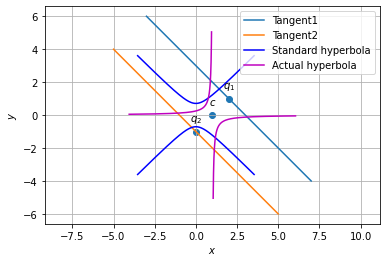
\includegraphics[width=\columnwidth]{./solutions/1/14/graph7.png}
	\caption{The standard and actual hyperbola.}
\end{figure}

%
\item    Balance the following chemical equation.
    \begin{align}
        \label{eq:solutions/chem/7b1} \text{Zinc + Silver nitrate} \to \text{Zinc nitrate + Silver}
    \end{align}
\solution
The given curve 
\begin{align}
	y =\frac{1}{x-1}
\end{align}
can be expressed as 
\begin{align}
	xy - y - 1 = 0 \label{eq:solutions/1/14/eq:hyperbola}
\end{align}
Hence, we have
\begin{align}
	\vec{V} = \frac{1}{2}\myvec{0 & 1 \\ 1 & 0}, 
	\vec{u} = \frac{1}{2}\myvec{0 \\-1},
	f = -1
\end{align}
Since $\mydet{\vec{V}} < 0$, the equation \eqref{eq:solutions/1/14/eq:hyperbola} represents hyperbola.
To find the values of $\lambda_1$ and $\lambda_2$, consider the characteristic equation,
\begin{align}
	\mydet{\lambda\vec{I} - \vec{V}} &= 0\\
	\implies \mydet{\myvec{\lambda & 0\\0 & \lambda} - \myvec{0 & \frac{1}{2} \\ \frac{1}{2} & 0}} &= 0\\
	\implies \mydet{ \lambda & \frac{-1}{2} \\ \frac{-1}{2} & \lambda} &= 0\\
	\implies \lambda_1 &= \frac{1}{2} , \lambda_2 = \frac{-1}{2}
\end{align}
In addition, given the slope -1, the direction and normal vectors are given by 
\begin{align}
	\vec{m} = \myvec{1 \\ -1} \\
	\vec{n} = \myvec{ 1 \\ 1}
\end{align}
The parameters of hyperbola are as follows:
\begin{align}
	\vec{c} &= -\vec{V}^{-1}\vec{u} \\
	&= -\myvec{0 & 2\\ 2 & 0}\myvec{0 \\ -\frac{1}{2}} \\
	&= \myvec{1 \\ 0}\\
	axes &= \begin{cases}
	\sqrt{\frac{\vec{u}^T\vec{V}^{-1}\vec{u} - f}{\lambda_1}} = \sqrt{2}\\
 \sqrt{\frac{f-\vec{u}^T\vec{V}^{-1}\vec{u}}{\lambda_2}} = \sqrt{2}
\end{cases}
\end{align}
which represents the standard hyperbola equation,
\begin{align}
	\frac{x^2}{2} - \frac{x^2}{2} = 1
\end{align}
The points of contact are given by 
\begin{align}
  \tiny{K} &=\pm \sqrt{\frac{\vec{u}^T\vec{V}^{-1}\vec{u} - f}{\vec{n}^T\vec{V}^{-1}\vec{n}}}
  = \pm \frac{1}{2}\\
  \vec{q} &= \vec{V}^{-1}(k\vec{n}-\vec{u})\\
  \vec{q_1} &= \myvec{0 & 2\\2 & 0} \sbrak{\frac{1}{2}\myvec{1 \\ 1} - \myvec{0\\ \frac{-1}{2}}}\\
  &= \myvec{2 \\ 1}\\
  \vec{q_2} &= \myvec{0 & 2\\2 & 0} \sbrak{\frac{-1}{2}\myvec{1 \\ 1} - \myvec{0\\ \frac{-1}{2}}}\\
  &= \myvec{0 \\ -1}
\end{align} 
$\therefore$ The tangents are given by
\begin{align}
	\myvec{1 & 1} \brak{\vec{x} - \myvec{2 \\ 1}} = 0 \\
	\myvec{1 & 1} \brak{\vec{x} - \myvec{0 \\ -1}} = 0
\end{align}
The desired equations of all lines having slope -1 that are tangents to the curve $\frac{1}{x-1}, x \neq 1$ are given by
\begin{align}
	\myvec{1 & 1}\vec{x} &= 3 \\
	\myvec{1 & 1}\vec{x} &= -1 
\end{align}
The above results are verified in the following figure.
\begin{figure}[h!] \label{eq:solutions/1/14/fig:tangents}
	\centering
	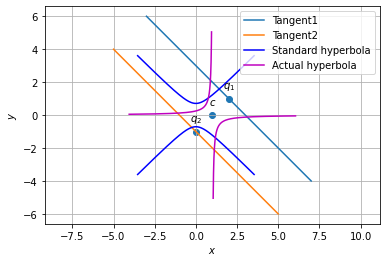
\includegraphics[width=\columnwidth]{./solutions/1/14/graph7.png}
	\caption{The standard and actual hyperbola.}
\end{figure}


\item Write the balanced chemical equations for the following reaction :
\begin{align}
 BaCl_2 + K_2SO_4 \rightarrow BaSO_4 + KCl \label{eq:solutions/chemistry/7d:1}   
\end{align}
\solution
The given curve 
\begin{align}
	y =\frac{1}{x-1}
\end{align}
can be expressed as 
\begin{align}
	xy - y - 1 = 0 \label{eq:solutions/1/14/eq:hyperbola}
\end{align}
Hence, we have
\begin{align}
	\vec{V} = \frac{1}{2}\myvec{0 & 1 \\ 1 & 0}, 
	\vec{u} = \frac{1}{2}\myvec{0 \\-1},
	f = -1
\end{align}
Since $\mydet{\vec{V}} < 0$, the equation \eqref{eq:solutions/1/14/eq:hyperbola} represents hyperbola.
To find the values of $\lambda_1$ and $\lambda_2$, consider the characteristic equation,
\begin{align}
	\mydet{\lambda\vec{I} - \vec{V}} &= 0\\
	\implies \mydet{\myvec{\lambda & 0\\0 & \lambda} - \myvec{0 & \frac{1}{2} \\ \frac{1}{2} & 0}} &= 0\\
	\implies \mydet{ \lambda & \frac{-1}{2} \\ \frac{-1}{2} & \lambda} &= 0\\
	\implies \lambda_1 &= \frac{1}{2} , \lambda_2 = \frac{-1}{2}
\end{align}
In addition, given the slope -1, the direction and normal vectors are given by 
\begin{align}
	\vec{m} = \myvec{1 \\ -1} \\
	\vec{n} = \myvec{ 1 \\ 1}
\end{align}
The parameters of hyperbola are as follows:
\begin{align}
	\vec{c} &= -\vec{V}^{-1}\vec{u} \\
	&= -\myvec{0 & 2\\ 2 & 0}\myvec{0 \\ -\frac{1}{2}} \\
	&= \myvec{1 \\ 0}\\
	axes &= \begin{cases}
	\sqrt{\frac{\vec{u}^T\vec{V}^{-1}\vec{u} - f}{\lambda_1}} = \sqrt{2}\\
 \sqrt{\frac{f-\vec{u}^T\vec{V}^{-1}\vec{u}}{\lambda_2}} = \sqrt{2}
\end{cases}
\end{align}
which represents the standard hyperbola equation,
\begin{align}
	\frac{x^2}{2} - \frac{x^2}{2} = 1
\end{align}
The points of contact are given by 
\begin{align}
  \tiny{K} &=\pm \sqrt{\frac{\vec{u}^T\vec{V}^{-1}\vec{u} - f}{\vec{n}^T\vec{V}^{-1}\vec{n}}}
  = \pm \frac{1}{2}\\
  \vec{q} &= \vec{V}^{-1}(k\vec{n}-\vec{u})\\
  \vec{q_1} &= \myvec{0 & 2\\2 & 0} \sbrak{\frac{1}{2}\myvec{1 \\ 1} - \myvec{0\\ \frac{-1}{2}}}\\
  &= \myvec{2 \\ 1}\\
  \vec{q_2} &= \myvec{0 & 2\\2 & 0} \sbrak{\frac{-1}{2}\myvec{1 \\ 1} - \myvec{0\\ \frac{-1}{2}}}\\
  &= \myvec{0 \\ -1}
\end{align} 
$\therefore$ The tangents are given by
\begin{align}
	\myvec{1 & 1} \brak{\vec{x} - \myvec{2 \\ 1}} = 0 \\
	\myvec{1 & 1} \brak{\vec{x} - \myvec{0 \\ -1}} = 0
\end{align}
The desired equations of all lines having slope -1 that are tangents to the curve $\frac{1}{x-1}, x \neq 1$ are given by
\begin{align}
	\myvec{1 & 1}\vec{x} &= 3 \\
	\myvec{1 & 1}\vec{x} &= -1 
\end{align}
The above results are verified in the following figure.
\begin{figure}[h!] \label{eq:solutions/1/14/fig:tangents}
	\centering
	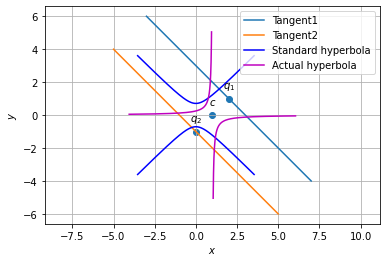
\includegraphics[width=\columnwidth]{./solutions/1/14/graph7.png}
	\caption{The standard and actual hyperbola.}
\end{figure}

%

%\end{enumerate}

%	
%\renewcommand{\theequation}{\theenumi}
%\begin{enumerate}[label=\arabic*.,ref=\thesubsection.\theenumi]
%\numberwithin{equation}{enumi}

\item Balance the following chemical equation.
%
\begin{align}
\label{eq:chem_balance}
Fe+H_2O &\rightarrow Fe_3O_4 + H_2
\end{align}
%
\solution Let the balanced version of \eqref{eq:chem_balance} be 
%
\begin{align}
\label{eq:chem_balance_unsol}
x_1Fe+x_2H_2 O &\rightarrow x_3Fe_3 O_4 + x_4H_2
\end{align}
%
which results in the following equations
%
\begin{align}
\begin{split}
\brak{x_1 -3x_3}Fe &= 0
\\
\brak{2x_2 -2x_4}H &= 0
\\
\brak{x_2 -4x_3}O &= 0
\end{split}
\end{align}
which can be expressed as
\begin{align}
\begin{split}
x_1 + 0.x_2 -3x_3 +0.x_4&= 0
\\
0.x_1+2x_2 +0.x_3-2x_4 &= 0
\\
0.x_1+x_2 -4x_3+ 0.x_4 &= 0
\end{split}
\end{align}
%
resulting in the matrix equation
\begin{align}
\label{eq:chem_balance_mat_eq}
\begin{split}
\myvec{
1 & 0 & -3 & 0
\\
0 & 2 & 0 & -2
\\
0 & 1 & -4 & 0
}
\vec{x} &= \vec{0}
\end{split}
\end{align}
%
where
\begin{align}
\vec{x} = \myvec{x_1 \\ x_2 \\ x_3 \\ x_4} 
\end{align}
%\item Solve \eqref{eq:chem_balance_unsol} by row reducing 
%the matrix in \eqref{eq:chem_balance_mat_eq}.
%\\
%\solution  
\eqref{eq:chem_balance_mat_eq} can be row reduced as follows
%
\begin{align}
\label{eq:chem_balance_mat_row}
\myvec{
1 & 0 & -3 & 0
\\
0 & 2 & 0 & -2
\\
0 & 1 & -4 & 0
}
 \xleftrightarrow[]{R_2 \leftarrow \frac{R_2}{2}}
\myvec{
1 & 0 & -3 & 0
\\
0 & 1 & 0 & -1
\\
0 & 1 & -4 & 0
}
\\
 \xleftrightarrow[]{R_3\leftarrow R_3-R_2}
\myvec{
1 & 0 & -3 & 0
\\
0 & 1 & 0 & -1
\\
0 & 0 & -4 & 1
}
\\
 \xleftrightarrow[]{R_1\leftarrow 4R_1-3R_3}
\myvec{
4 & 0 & 0 & -3
\\
0 & 1 & 0 & -1
\\
0 & 0 & -4 & 1
}
\\
 \xleftrightarrow[R_3 \leftarrow -\frac{1}{4}R_3]{R_1\leftarrow \frac{1}{4}}
\myvec{
1 & 0 & 0 & -\frac{3}{4}
\\
0 & 1 & 0 & -1
\\
0 & 0 & 1 & -\frac{1}{4}
}
\end{align}
%
Thus, 
\begin{align}
\label{eq:chem_balance_mat_sol}
x_1 &= \frac{3}{4}x_4, x_2 = x_4, x_3 = \frac{1}{4}x_4
\\
\\
\implies 
\vec{x} &= x_4\myvec{\frac{3}{4} \\ 1 \\ \frac{1}{4} \\ 1}= \myvec{3 \\ 4 \\ 1 \\ 4}
\end{align}
%
upon substituting $x_4 = 4$.
%
\eqref{eq:chem_balance_unsol} then becomes
%
\begin{align}
\label{eq:chem_balance_final}
3Fe+4H_2 O &\rightarrow Fe_3 O_4 + 4H_2
\end{align}

\item Consider the following information regarding the number of men and women workers in the three factories I,II and III

\begin{tabular}{ |c|c|c| } 
\hline
 & Men Workers & Women Workers \\
\hline
\multirow{3}{4em}{I \\II \\III} & 30 & 25\\ 
& 25 & 31 \\ 
&27 & 26 \\ 
\hline
\end{tabular}\\
Represent the above information in the form of a 3 $\times$ 2 matrix. What does the entry
in the third row and second column represent?\\


 \item  If a matrix has 8 elements, what are the possible orders it can have?\\
    \item Construct a 3 $\times$ 2 matrix whose elements are given by $a_{ij}=\frac{1}{2}\abs{i-3j}$\\
    \item \myvec{x+3 &z+4 &2y-7\\-6 &a-1 &0\\b-3 &-21 &0}=\myvec{0 &6 &3y-2\\-6 &-3 &2c+2\\2b+4 &-21 &0}\\
    Find the values of a,b,c,x,y and z.\\
\solution 
 As the two matrices are equal their corresponding entries are also equal. Hence
\begin{align}
x+3&=0 \quad \implies x=-3
\\
z+4&=6 \quad \implies z=2
\\
2y-7&=3y-2 \quad \implies y=-5
\\
a-1&=-3 \quad \implies a=-2
\\
2c+2&=0 \quad \implies c=-1
\\
b-3&=2b+4 \quad \implies b=-7
\end{align}

    \item Find the values of a,b,c and d from the following equation:\\
    \myvec{2a+b &a-2b\\5c-d &4c+3d}=\myvec{4 &-3\\11 &24}\\
\solution 
The given curve 
\begin{align}
	y =\frac{1}{x-1}
\end{align}
can be expressed as 
\begin{align}
	xy - y - 1 = 0 \label{eq:solutions/1/14/eq:hyperbola}
\end{align}
Hence, we have
\begin{align}
	\vec{V} = \frac{1}{2}\myvec{0 & 1 \\ 1 & 0}, 
	\vec{u} = \frac{1}{2}\myvec{0 \\-1},
	f = -1
\end{align}
Since $\mydet{\vec{V}} < 0$, the equation \eqref{eq:solutions/1/14/eq:hyperbola} represents hyperbola.
To find the values of $\lambda_1$ and $\lambda_2$, consider the characteristic equation,
\begin{align}
	\mydet{\lambda\vec{I} - \vec{V}} &= 0\\
	\implies \mydet{\myvec{\lambda & 0\\0 & \lambda} - \myvec{0 & \frac{1}{2} \\ \frac{1}{2} & 0}} &= 0\\
	\implies \mydet{ \lambda & \frac{-1}{2} \\ \frac{-1}{2} & \lambda} &= 0\\
	\implies \lambda_1 &= \frac{1}{2} , \lambda_2 = \frac{-1}{2}
\end{align}
In addition, given the slope -1, the direction and normal vectors are given by 
\begin{align}
	\vec{m} = \myvec{1 \\ -1} \\
	\vec{n} = \myvec{ 1 \\ 1}
\end{align}
The parameters of hyperbola are as follows:
\begin{align}
	\vec{c} &= -\vec{V}^{-1}\vec{u} \\
	&= -\myvec{0 & 2\\ 2 & 0}\myvec{0 \\ -\frac{1}{2}} \\
	&= \myvec{1 \\ 0}\\
	axes &= \begin{cases}
	\sqrt{\frac{\vec{u}^T\vec{V}^{-1}\vec{u} - f}{\lambda_1}} = \sqrt{2}\\
 \sqrt{\frac{f-\vec{u}^T\vec{V}^{-1}\vec{u}}{\lambda_2}} = \sqrt{2}
\end{cases}
\end{align}
which represents the standard hyperbola equation,
\begin{align}
	\frac{x^2}{2} - \frac{x^2}{2} = 1
\end{align}
The points of contact are given by 
\begin{align}
  \tiny{K} &=\pm \sqrt{\frac{\vec{u}^T\vec{V}^{-1}\vec{u} - f}{\vec{n}^T\vec{V}^{-1}\vec{n}}}
  = \pm \frac{1}{2}\\
  \vec{q} &= \vec{V}^{-1}(k\vec{n}-\vec{u})\\
  \vec{q_1} &= \myvec{0 & 2\\2 & 0} \sbrak{\frac{1}{2}\myvec{1 \\ 1} - \myvec{0\\ \frac{-1}{2}}}\\
  &= \myvec{2 \\ 1}\\
  \vec{q_2} &= \myvec{0 & 2\\2 & 0} \sbrak{\frac{-1}{2}\myvec{1 \\ 1} - \myvec{0\\ \frac{-1}{2}}}\\
  &= \myvec{0 \\ -1}
\end{align} 
$\therefore$ The tangents are given by
\begin{align}
	\myvec{1 & 1} \brak{\vec{x} - \myvec{2 \\ 1}} = 0 \\
	\myvec{1 & 1} \brak{\vec{x} - \myvec{0 \\ -1}} = 0
\end{align}
The desired equations of all lines having slope -1 that are tangents to the curve $\frac{1}{x-1}, x \neq 1$ are given by
\begin{align}
	\myvec{1 & 1}\vec{x} &= 3 \\
	\myvec{1 & 1}\vec{x} &= -1 
\end{align}
The above results are verified in the following figure.
\begin{figure}[h!] \label{eq:solutions/1/14/fig:tangents}
	\centering
	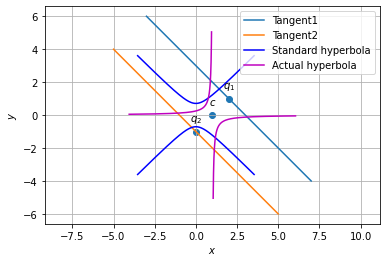
\includegraphics[width=\columnwidth]{./solutions/1/14/graph7.png}
	\caption{The standard and actual hyperbola.}
\end{figure}

    \item Given A=\myvec{\sqrt{3} &1 &-1\\2 &3 &0} and B=\myvec{2 &\sqrt{5} &1\\-2 &3 &\frac{1}{2}}, find A+B.\\\solution 
The given curve 
\begin{align}
	y =\frac{1}{x-1}
\end{align}
can be expressed as 
\begin{align}
	xy - y - 1 = 0 \label{eq:solutions/1/14/eq:hyperbola}
\end{align}
Hence, we have
\begin{align}
	\vec{V} = \frac{1}{2}\myvec{0 & 1 \\ 1 & 0}, 
	\vec{u} = \frac{1}{2}\myvec{0 \\-1},
	f = -1
\end{align}
Since $\mydet{\vec{V}} < 0$, the equation \eqref{eq:solutions/1/14/eq:hyperbola} represents hyperbola.
To find the values of $\lambda_1$ and $\lambda_2$, consider the characteristic equation,
\begin{align}
	\mydet{\lambda\vec{I} - \vec{V}} &= 0\\
	\implies \mydet{\myvec{\lambda & 0\\0 & \lambda} - \myvec{0 & \frac{1}{2} \\ \frac{1}{2} & 0}} &= 0\\
	\implies \mydet{ \lambda & \frac{-1}{2} \\ \frac{-1}{2} & \lambda} &= 0\\
	\implies \lambda_1 &= \frac{1}{2} , \lambda_2 = \frac{-1}{2}
\end{align}
In addition, given the slope -1, the direction and normal vectors are given by 
\begin{align}
	\vec{m} = \myvec{1 \\ -1} \\
	\vec{n} = \myvec{ 1 \\ 1}
\end{align}
The parameters of hyperbola are as follows:
\begin{align}
	\vec{c} &= -\vec{V}^{-1}\vec{u} \\
	&= -\myvec{0 & 2\\ 2 & 0}\myvec{0 \\ -\frac{1}{2}} \\
	&= \myvec{1 \\ 0}\\
	axes &= \begin{cases}
	\sqrt{\frac{\vec{u}^T\vec{V}^{-1}\vec{u} - f}{\lambda_1}} = \sqrt{2}\\
 \sqrt{\frac{f-\vec{u}^T\vec{V}^{-1}\vec{u}}{\lambda_2}} = \sqrt{2}
\end{cases}
\end{align}
which represents the standard hyperbola equation,
\begin{align}
	\frac{x^2}{2} - \frac{x^2}{2} = 1
\end{align}
The points of contact are given by 
\begin{align}
  \tiny{K} &=\pm \sqrt{\frac{\vec{u}^T\vec{V}^{-1}\vec{u} - f}{\vec{n}^T\vec{V}^{-1}\vec{n}}}
  = \pm \frac{1}{2}\\
  \vec{q} &= \vec{V}^{-1}(k\vec{n}-\vec{u})\\
  \vec{q_1} &= \myvec{0 & 2\\2 & 0} \sbrak{\frac{1}{2}\myvec{1 \\ 1} - \myvec{0\\ \frac{-1}{2}}}\\
  &= \myvec{2 \\ 1}\\
  \vec{q_2} &= \myvec{0 & 2\\2 & 0} \sbrak{\frac{-1}{2}\myvec{1 \\ 1} - \myvec{0\\ \frac{-1}{2}}}\\
  &= \myvec{0 \\ -1}
\end{align} 
$\therefore$ The tangents are given by
\begin{align}
	\myvec{1 & 1} \brak{\vec{x} - \myvec{2 \\ 1}} = 0 \\
	\myvec{1 & 1} \brak{\vec{x} - \myvec{0 \\ -1}} = 0
\end{align}
The desired equations of all lines having slope -1 that are tangents to the curve $\frac{1}{x-1}, x \neq 1$ are given by
\begin{align}
	\myvec{1 & 1}\vec{x} &= 3 \\
	\myvec{1 & 1}\vec{x} &= -1 
\end{align}
The above results are verified in the following figure.
\begin{figure}[h!] \label{eq:solutions/1/14/fig:tangents}
	\centering
	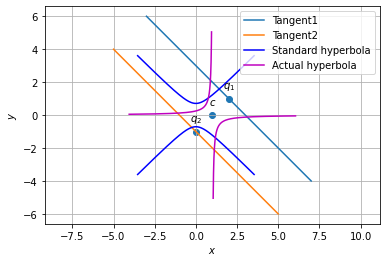
\includegraphics[width=\columnwidth]{./solutions/1/14/graph7.png}
	\caption{The standard and actual hyperbola.}
\end{figure}

\item In the matrix A=\myvec{2 &5 &19 &-7\\ 35 &-2 &\frac{5}{2} &12 \\ \sqrt{3} &1 &-5 &17}, write
\begin{enumerate}
\item The order of the matrix
\item The number of elements
\item Write the elements $a_{31},a_{21},a_{33},a_{24},a_{23}.$
\end{enumerate}
\solution 
The given curve 
\begin{align}
	y =\frac{1}{x-1}
\end{align}
can be expressed as 
\begin{align}
	xy - y - 1 = 0 \label{eq:solutions/1/14/eq:hyperbola}
\end{align}
Hence, we have
\begin{align}
	\vec{V} = \frac{1}{2}\myvec{0 & 1 \\ 1 & 0}, 
	\vec{u} = \frac{1}{2}\myvec{0 \\-1},
	f = -1
\end{align}
Since $\mydet{\vec{V}} < 0$, the equation \eqref{eq:solutions/1/14/eq:hyperbola} represents hyperbola.
To find the values of $\lambda_1$ and $\lambda_2$, consider the characteristic equation,
\begin{align}
	\mydet{\lambda\vec{I} - \vec{V}} &= 0\\
	\implies \mydet{\myvec{\lambda & 0\\0 & \lambda} - \myvec{0 & \frac{1}{2} \\ \frac{1}{2} & 0}} &= 0\\
	\implies \mydet{ \lambda & \frac{-1}{2} \\ \frac{-1}{2} & \lambda} &= 0\\
	\implies \lambda_1 &= \frac{1}{2} , \lambda_2 = \frac{-1}{2}
\end{align}
In addition, given the slope -1, the direction and normal vectors are given by 
\begin{align}
	\vec{m} = \myvec{1 \\ -1} \\
	\vec{n} = \myvec{ 1 \\ 1}
\end{align}
The parameters of hyperbola are as follows:
\begin{align}
	\vec{c} &= -\vec{V}^{-1}\vec{u} \\
	&= -\myvec{0 & 2\\ 2 & 0}\myvec{0 \\ -\frac{1}{2}} \\
	&= \myvec{1 \\ 0}\\
	axes &= \begin{cases}
	\sqrt{\frac{\vec{u}^T\vec{V}^{-1}\vec{u} - f}{\lambda_1}} = \sqrt{2}\\
 \sqrt{\frac{f-\vec{u}^T\vec{V}^{-1}\vec{u}}{\lambda_2}} = \sqrt{2}
\end{cases}
\end{align}
which represents the standard hyperbola equation,
\begin{align}
	\frac{x^2}{2} - \frac{x^2}{2} = 1
\end{align}
The points of contact are given by 
\begin{align}
  \tiny{K} &=\pm \sqrt{\frac{\vec{u}^T\vec{V}^{-1}\vec{u} - f}{\vec{n}^T\vec{V}^{-1}\vec{n}}}
  = \pm \frac{1}{2}\\
  \vec{q} &= \vec{V}^{-1}(k\vec{n}-\vec{u})\\
  \vec{q_1} &= \myvec{0 & 2\\2 & 0} \sbrak{\frac{1}{2}\myvec{1 \\ 1} - \myvec{0\\ \frac{-1}{2}}}\\
  &= \myvec{2 \\ 1}\\
  \vec{q_2} &= \myvec{0 & 2\\2 & 0} \sbrak{\frac{-1}{2}\myvec{1 \\ 1} - \myvec{0\\ \frac{-1}{2}}}\\
  &= \myvec{0 \\ -1}
\end{align} 
$\therefore$ The tangents are given by
\begin{align}
	\myvec{1 & 1} \brak{\vec{x} - \myvec{2 \\ 1}} = 0 \\
	\myvec{1 & 1} \brak{\vec{x} - \myvec{0 \\ -1}} = 0
\end{align}
The desired equations of all lines having slope -1 that are tangents to the curve $\frac{1}{x-1}, x \neq 1$ are given by
\begin{align}
	\myvec{1 & 1}\vec{x} &= 3 \\
	\myvec{1 & 1}\vec{x} &= -1 
\end{align}
The above results are verified in the following figure.
\begin{figure}[h!] \label{eq:solutions/1/14/fig:tangents}
	\centering
	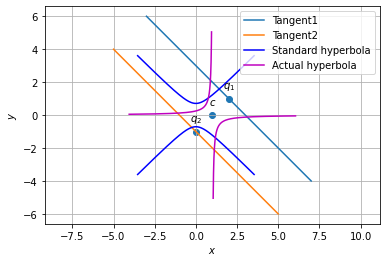
\includegraphics[width=\columnwidth]{./solutions/1/14/graph7.png}
	\caption{The standard and actual hyperbola.}
\end{figure}


\item If a matrix has 24 elements,what are the possible orders it can have? What,if it has 13 elements?\\
\solution 
The given curve 
\begin{align}
	y =\frac{1}{x-1}
\end{align}
can be expressed as 
\begin{align}
	xy - y - 1 = 0 \label{eq:solutions/1/14/eq:hyperbola}
\end{align}
Hence, we have
\begin{align}
	\vec{V} = \frac{1}{2}\myvec{0 & 1 \\ 1 & 0}, 
	\vec{u} = \frac{1}{2}\myvec{0 \\-1},
	f = -1
\end{align}
Since $\mydet{\vec{V}} < 0$, the equation \eqref{eq:solutions/1/14/eq:hyperbola} represents hyperbola.
To find the values of $\lambda_1$ and $\lambda_2$, consider the characteristic equation,
\begin{align}
	\mydet{\lambda\vec{I} - \vec{V}} &= 0\\
	\implies \mydet{\myvec{\lambda & 0\\0 & \lambda} - \myvec{0 & \frac{1}{2} \\ \frac{1}{2} & 0}} &= 0\\
	\implies \mydet{ \lambda & \frac{-1}{2} \\ \frac{-1}{2} & \lambda} &= 0\\
	\implies \lambda_1 &= \frac{1}{2} , \lambda_2 = \frac{-1}{2}
\end{align}
In addition, given the slope -1, the direction and normal vectors are given by 
\begin{align}
	\vec{m} = \myvec{1 \\ -1} \\
	\vec{n} = \myvec{ 1 \\ 1}
\end{align}
The parameters of hyperbola are as follows:
\begin{align}
	\vec{c} &= -\vec{V}^{-1}\vec{u} \\
	&= -\myvec{0 & 2\\ 2 & 0}\myvec{0 \\ -\frac{1}{2}} \\
	&= \myvec{1 \\ 0}\\
	axes &= \begin{cases}
	\sqrt{\frac{\vec{u}^T\vec{V}^{-1}\vec{u} - f}{\lambda_1}} = \sqrt{2}\\
 \sqrt{\frac{f-\vec{u}^T\vec{V}^{-1}\vec{u}}{\lambda_2}} = \sqrt{2}
\end{cases}
\end{align}
which represents the standard hyperbola equation,
\begin{align}
	\frac{x^2}{2} - \frac{x^2}{2} = 1
\end{align}
The points of contact are given by 
\begin{align}
  \tiny{K} &=\pm \sqrt{\frac{\vec{u}^T\vec{V}^{-1}\vec{u} - f}{\vec{n}^T\vec{V}^{-1}\vec{n}}}
  = \pm \frac{1}{2}\\
  \vec{q} &= \vec{V}^{-1}(k\vec{n}-\vec{u})\\
  \vec{q_1} &= \myvec{0 & 2\\2 & 0} \sbrak{\frac{1}{2}\myvec{1 \\ 1} - \myvec{0\\ \frac{-1}{2}}}\\
  &= \myvec{2 \\ 1}\\
  \vec{q_2} &= \myvec{0 & 2\\2 & 0} \sbrak{\frac{-1}{2}\myvec{1 \\ 1} - \myvec{0\\ \frac{-1}{2}}}\\
  &= \myvec{0 \\ -1}
\end{align} 
$\therefore$ The tangents are given by
\begin{align}
	\myvec{1 & 1} \brak{\vec{x} - \myvec{2 \\ 1}} = 0 \\
	\myvec{1 & 1} \brak{\vec{x} - \myvec{0 \\ -1}} = 0
\end{align}
The desired equations of all lines having slope -1 that are tangents to the curve $\frac{1}{x-1}, x \neq 1$ are given by
\begin{align}
	\myvec{1 & 1}\vec{x} &= 3 \\
	\myvec{1 & 1}\vec{x} &= -1 
\end{align}
The above results are verified in the following figure.
\begin{figure}[h!] \label{eq:solutions/1/14/fig:tangents}
	\centering
	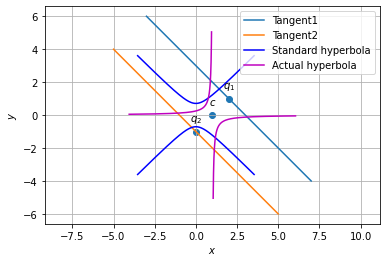
\includegraphics[width=\columnwidth]{./solutions/1/14/graph7.png}
	\caption{The standard and actual hyperbola.}
\end{figure}

\item If a matrix has 18 elements,what are the possible orders it can have? What,if it has 5 elements?\\
\\
\solution 
The given curve 
\begin{align}
	y =\frac{1}{x-1}
\end{align}
can be expressed as 
\begin{align}
	xy - y - 1 = 0 \label{eq:solutions/1/14/eq:hyperbola}
\end{align}
Hence, we have
\begin{align}
	\vec{V} = \frac{1}{2}\myvec{0 & 1 \\ 1 & 0}, 
	\vec{u} = \frac{1}{2}\myvec{0 \\-1},
	f = -1
\end{align}
Since $\mydet{\vec{V}} < 0$, the equation \eqref{eq:solutions/1/14/eq:hyperbola} represents hyperbola.
To find the values of $\lambda_1$ and $\lambda_2$, consider the characteristic equation,
\begin{align}
	\mydet{\lambda\vec{I} - \vec{V}} &= 0\\
	\implies \mydet{\myvec{\lambda & 0\\0 & \lambda} - \myvec{0 & \frac{1}{2} \\ \frac{1}{2} & 0}} &= 0\\
	\implies \mydet{ \lambda & \frac{-1}{2} \\ \frac{-1}{2} & \lambda} &= 0\\
	\implies \lambda_1 &= \frac{1}{2} , \lambda_2 = \frac{-1}{2}
\end{align}
In addition, given the slope -1, the direction and normal vectors are given by 
\begin{align}
	\vec{m} = \myvec{1 \\ -1} \\
	\vec{n} = \myvec{ 1 \\ 1}
\end{align}
The parameters of hyperbola are as follows:
\begin{align}
	\vec{c} &= -\vec{V}^{-1}\vec{u} \\
	&= -\myvec{0 & 2\\ 2 & 0}\myvec{0 \\ -\frac{1}{2}} \\
	&= \myvec{1 \\ 0}\\
	axes &= \begin{cases}
	\sqrt{\frac{\vec{u}^T\vec{V}^{-1}\vec{u} - f}{\lambda_1}} = \sqrt{2}\\
 \sqrt{\frac{f-\vec{u}^T\vec{V}^{-1}\vec{u}}{\lambda_2}} = \sqrt{2}
\end{cases}
\end{align}
which represents the standard hyperbola equation,
\begin{align}
	\frac{x^2}{2} - \frac{x^2}{2} = 1
\end{align}
The points of contact are given by 
\begin{align}
  \tiny{K} &=\pm \sqrt{\frac{\vec{u}^T\vec{V}^{-1}\vec{u} - f}{\vec{n}^T\vec{V}^{-1}\vec{n}}}
  = \pm \frac{1}{2}\\
  \vec{q} &= \vec{V}^{-1}(k\vec{n}-\vec{u})\\
  \vec{q_1} &= \myvec{0 & 2\\2 & 0} \sbrak{\frac{1}{2}\myvec{1 \\ 1} - \myvec{0\\ \frac{-1}{2}}}\\
  &= \myvec{2 \\ 1}\\
  \vec{q_2} &= \myvec{0 & 2\\2 & 0} \sbrak{\frac{-1}{2}\myvec{1 \\ 1} - \myvec{0\\ \frac{-1}{2}}}\\
  &= \myvec{0 \\ -1}
\end{align} 
$\therefore$ The tangents are given by
\begin{align}
	\myvec{1 & 1} \brak{\vec{x} - \myvec{2 \\ 1}} = 0 \\
	\myvec{1 & 1} \brak{\vec{x} - \myvec{0 \\ -1}} = 0
\end{align}
The desired equations of all lines having slope -1 that are tangents to the curve $\frac{1}{x-1}, x \neq 1$ are given by
\begin{align}
	\myvec{1 & 1}\vec{x} &= 3 \\
	\myvec{1 & 1}\vec{x} &= -1 
\end{align}
The above results are verified in the following figure.
\begin{figure}[h!] \label{eq:solutions/1/14/fig:tangents}
	\centering
	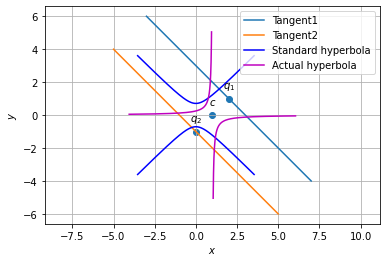
\includegraphics[width=\columnwidth]{./solutions/1/14/graph7.png}
	\caption{The standard and actual hyperbola.}
\end{figure}

%
\item Construct a $2 \times 2$ matrix,A=[$a_{ij}$],whose elements are given by:\\
(i) $a_{ij}$=$\frac{(i+j)^2}{2}$\ (ii) $a_{ij}$=$\frac{i}{j}$\ (iii) $a_{ij}$=$\frac{(i+2j)^2}{2}$\\
\solution 
The given curve 
\begin{align}
	y =\frac{1}{x-1}
\end{align}
can be expressed as 
\begin{align}
	xy - y - 1 = 0 \label{eq:solutions/1/14/eq:hyperbola}
\end{align}
Hence, we have
\begin{align}
	\vec{V} = \frac{1}{2}\myvec{0 & 1 \\ 1 & 0}, 
	\vec{u} = \frac{1}{2}\myvec{0 \\-1},
	f = -1
\end{align}
Since $\mydet{\vec{V}} < 0$, the equation \eqref{eq:solutions/1/14/eq:hyperbola} represents hyperbola.
To find the values of $\lambda_1$ and $\lambda_2$, consider the characteristic equation,
\begin{align}
	\mydet{\lambda\vec{I} - \vec{V}} &= 0\\
	\implies \mydet{\myvec{\lambda & 0\\0 & \lambda} - \myvec{0 & \frac{1}{2} \\ \frac{1}{2} & 0}} &= 0\\
	\implies \mydet{ \lambda & \frac{-1}{2} \\ \frac{-1}{2} & \lambda} &= 0\\
	\implies \lambda_1 &= \frac{1}{2} , \lambda_2 = \frac{-1}{2}
\end{align}
In addition, given the slope -1, the direction and normal vectors are given by 
\begin{align}
	\vec{m} = \myvec{1 \\ -1} \\
	\vec{n} = \myvec{ 1 \\ 1}
\end{align}
The parameters of hyperbola are as follows:
\begin{align}
	\vec{c} &= -\vec{V}^{-1}\vec{u} \\
	&= -\myvec{0 & 2\\ 2 & 0}\myvec{0 \\ -\frac{1}{2}} \\
	&= \myvec{1 \\ 0}\\
	axes &= \begin{cases}
	\sqrt{\frac{\vec{u}^T\vec{V}^{-1}\vec{u} - f}{\lambda_1}} = \sqrt{2}\\
 \sqrt{\frac{f-\vec{u}^T\vec{V}^{-1}\vec{u}}{\lambda_2}} = \sqrt{2}
\end{cases}
\end{align}
which represents the standard hyperbola equation,
\begin{align}
	\frac{x^2}{2} - \frac{x^2}{2} = 1
\end{align}
The points of contact are given by 
\begin{align}
  \tiny{K} &=\pm \sqrt{\frac{\vec{u}^T\vec{V}^{-1}\vec{u} - f}{\vec{n}^T\vec{V}^{-1}\vec{n}}}
  = \pm \frac{1}{2}\\
  \vec{q} &= \vec{V}^{-1}(k\vec{n}-\vec{u})\\
  \vec{q_1} &= \myvec{0 & 2\\2 & 0} \sbrak{\frac{1}{2}\myvec{1 \\ 1} - \myvec{0\\ \frac{-1}{2}}}\\
  &= \myvec{2 \\ 1}\\
  \vec{q_2} &= \myvec{0 & 2\\2 & 0} \sbrak{\frac{-1}{2}\myvec{1 \\ 1} - \myvec{0\\ \frac{-1}{2}}}\\
  &= \myvec{0 \\ -1}
\end{align} 
$\therefore$ The tangents are given by
\begin{align}
	\myvec{1 & 1} \brak{\vec{x} - \myvec{2 \\ 1}} = 0 \\
	\myvec{1 & 1} \brak{\vec{x} - \myvec{0 \\ -1}} = 0
\end{align}
The desired equations of all lines having slope -1 that are tangents to the curve $\frac{1}{x-1}, x \neq 1$ are given by
\begin{align}
	\myvec{1 & 1}\vec{x} &= 3 \\
	\myvec{1 & 1}\vec{x} &= -1 
\end{align}
The above results are verified in the following figure.
\begin{figure}[h!] \label{eq:solutions/1/14/fig:tangents}
	\centering
	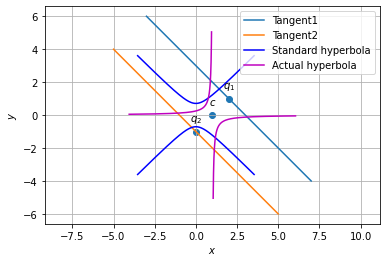
\includegraphics[width=\columnwidth]{./solutions/1/14/graph7.png}
	\caption{The standard and actual hyperbola.}
\end{figure}

\item Construct a $3\times 4$ matrix,whose elements are given by:\\
(i) $a_{ij}$=$\frac{1}{2}\abs{-3i+j}$ (ii) $a_{ij}$=2i-j\\
\solution 
	
	The following python code computes the required matrix.
	\begin{lstlisting}
	./codes/lines/q13.py
	\end{lstlisting}
	
	\begin{enumerate}
		\item The matrix $A_{ij} = \frac{1}{2}|-3i+j|$ obtained is
		\begin{align}
			\myvec{0&0.5&1&1.5\\1.5&1&0.5&0\\3&2.5&2&1.5}
		\end{align}
		\item The matrix $A_{ij} = 2i-j$ obtained is
		\begin{align}
			\myvec{0&-1&-2&-3\\2&1&0&-1\\4&3&2&1}
		\end{align}
	\end{enumerate}
	
	

\item Find the values of x,y and z from the following equations:\\
(i) \myvec{4 &3\\x &5} = \myvec{y &z\\1 &5} (ii) \myvec{x+y &2\\5+z &xy} = \myvec{6 &2\\5 &8} (iii) \myvec{x+y+z\\x+y\\y+z}=\myvec{9\\5\\7}\\
\\
\solution 
The given curve 
\begin{align}
	y =\frac{1}{x-1}
\end{align}
can be expressed as 
\begin{align}
	xy - y - 1 = 0 \label{eq:solutions/1/14/eq:hyperbola}
\end{align}
Hence, we have
\begin{align}
	\vec{V} = \frac{1}{2}\myvec{0 & 1 \\ 1 & 0}, 
	\vec{u} = \frac{1}{2}\myvec{0 \\-1},
	f = -1
\end{align}
Since $\mydet{\vec{V}} < 0$, the equation \eqref{eq:solutions/1/14/eq:hyperbola} represents hyperbola.
To find the values of $\lambda_1$ and $\lambda_2$, consider the characteristic equation,
\begin{align}
	\mydet{\lambda\vec{I} - \vec{V}} &= 0\\
	\implies \mydet{\myvec{\lambda & 0\\0 & \lambda} - \myvec{0 & \frac{1}{2} \\ \frac{1}{2} & 0}} &= 0\\
	\implies \mydet{ \lambda & \frac{-1}{2} \\ \frac{-1}{2} & \lambda} &= 0\\
	\implies \lambda_1 &= \frac{1}{2} , \lambda_2 = \frac{-1}{2}
\end{align}
In addition, given the slope -1, the direction and normal vectors are given by 
\begin{align}
	\vec{m} = \myvec{1 \\ -1} \\
	\vec{n} = \myvec{ 1 \\ 1}
\end{align}
The parameters of hyperbola are as follows:
\begin{align}
	\vec{c} &= -\vec{V}^{-1}\vec{u} \\
	&= -\myvec{0 & 2\\ 2 & 0}\myvec{0 \\ -\frac{1}{2}} \\
	&= \myvec{1 \\ 0}\\
	axes &= \begin{cases}
	\sqrt{\frac{\vec{u}^T\vec{V}^{-1}\vec{u} - f}{\lambda_1}} = \sqrt{2}\\
 \sqrt{\frac{f-\vec{u}^T\vec{V}^{-1}\vec{u}}{\lambda_2}} = \sqrt{2}
\end{cases}
\end{align}
which represents the standard hyperbola equation,
\begin{align}
	\frac{x^2}{2} - \frac{x^2}{2} = 1
\end{align}
The points of contact are given by 
\begin{align}
  \tiny{K} &=\pm \sqrt{\frac{\vec{u}^T\vec{V}^{-1}\vec{u} - f}{\vec{n}^T\vec{V}^{-1}\vec{n}}}
  = \pm \frac{1}{2}\\
  \vec{q} &= \vec{V}^{-1}(k\vec{n}-\vec{u})\\
  \vec{q_1} &= \myvec{0 & 2\\2 & 0} \sbrak{\frac{1}{2}\myvec{1 \\ 1} - \myvec{0\\ \frac{-1}{2}}}\\
  &= \myvec{2 \\ 1}\\
  \vec{q_2} &= \myvec{0 & 2\\2 & 0} \sbrak{\frac{-1}{2}\myvec{1 \\ 1} - \myvec{0\\ \frac{-1}{2}}}\\
  &= \myvec{0 \\ -1}
\end{align} 
$\therefore$ The tangents are given by
\begin{align}
	\myvec{1 & 1} \brak{\vec{x} - \myvec{2 \\ 1}} = 0 \\
	\myvec{1 & 1} \brak{\vec{x} - \myvec{0 \\ -1}} = 0
\end{align}
The desired equations of all lines having slope -1 that are tangents to the curve $\frac{1}{x-1}, x \neq 1$ are given by
\begin{align}
	\myvec{1 & 1}\vec{x} &= 3 \\
	\myvec{1 & 1}\vec{x} &= -1 
\end{align}
The above results are verified in the following figure.
\begin{figure}[h!] \label{eq:solutions/1/14/fig:tangents}
	\centering
	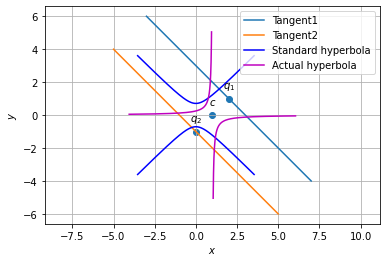
\includegraphics[width=\columnwidth]{./solutions/1/14/graph7.png}
	\caption{The standard and actual hyperbola.}
\end{figure}

\item Compute the indicated products.
\begin{enumerate}
\item \myvec{a &b\\-b &a}\myvec{a &-b\\b &a} \\
\solution 
The given curve 
\begin{align}
	y =\frac{1}{x-1}
\end{align}
can be expressed as 
\begin{align}
	xy - y - 1 = 0 \label{eq:solutions/1/14/eq:hyperbola}
\end{align}
Hence, we have
\begin{align}
	\vec{V} = \frac{1}{2}\myvec{0 & 1 \\ 1 & 0}, 
	\vec{u} = \frac{1}{2}\myvec{0 \\-1},
	f = -1
\end{align}
Since $\mydet{\vec{V}} < 0$, the equation \eqref{eq:solutions/1/14/eq:hyperbola} represents hyperbola.
To find the values of $\lambda_1$ and $\lambda_2$, consider the characteristic equation,
\begin{align}
	\mydet{\lambda\vec{I} - \vec{V}} &= 0\\
	\implies \mydet{\myvec{\lambda & 0\\0 & \lambda} - \myvec{0 & \frac{1}{2} \\ \frac{1}{2} & 0}} &= 0\\
	\implies \mydet{ \lambda & \frac{-1}{2} \\ \frac{-1}{2} & \lambda} &= 0\\
	\implies \lambda_1 &= \frac{1}{2} , \lambda_2 = \frac{-1}{2}
\end{align}
In addition, given the slope -1, the direction and normal vectors are given by 
\begin{align}
	\vec{m} = \myvec{1 \\ -1} \\
	\vec{n} = \myvec{ 1 \\ 1}
\end{align}
The parameters of hyperbola are as follows:
\begin{align}
	\vec{c} &= -\vec{V}^{-1}\vec{u} \\
	&= -\myvec{0 & 2\\ 2 & 0}\myvec{0 \\ -\frac{1}{2}} \\
	&= \myvec{1 \\ 0}\\
	axes &= \begin{cases}
	\sqrt{\frac{\vec{u}^T\vec{V}^{-1}\vec{u} - f}{\lambda_1}} = \sqrt{2}\\
 \sqrt{\frac{f-\vec{u}^T\vec{V}^{-1}\vec{u}}{\lambda_2}} = \sqrt{2}
\end{cases}
\end{align}
which represents the standard hyperbola equation,
\begin{align}
	\frac{x^2}{2} - \frac{x^2}{2} = 1
\end{align}
The points of contact are given by 
\begin{align}
  \tiny{K} &=\pm \sqrt{\frac{\vec{u}^T\vec{V}^{-1}\vec{u} - f}{\vec{n}^T\vec{V}^{-1}\vec{n}}}
  = \pm \frac{1}{2}\\
  \vec{q} &= \vec{V}^{-1}(k\vec{n}-\vec{u})\\
  \vec{q_1} &= \myvec{0 & 2\\2 & 0} \sbrak{\frac{1}{2}\myvec{1 \\ 1} - \myvec{0\\ \frac{-1}{2}}}\\
  &= \myvec{2 \\ 1}\\
  \vec{q_2} &= \myvec{0 & 2\\2 & 0} \sbrak{\frac{-1}{2}\myvec{1 \\ 1} - \myvec{0\\ \frac{-1}{2}}}\\
  &= \myvec{0 \\ -1}
\end{align} 
$\therefore$ The tangents are given by
\begin{align}
	\myvec{1 & 1} \brak{\vec{x} - \myvec{2 \\ 1}} = 0 \\
	\myvec{1 & 1} \brak{\vec{x} - \myvec{0 \\ -1}} = 0
\end{align}
The desired equations of all lines having slope -1 that are tangents to the curve $\frac{1}{x-1}, x \neq 1$ are given by
\begin{align}
	\myvec{1 & 1}\vec{x} &= 3 \\
	\myvec{1 & 1}\vec{x} &= -1 
\end{align}
The above results are verified in the following figure.
\begin{figure}[h!] \label{eq:solutions/1/14/fig:tangents}
	\centering
	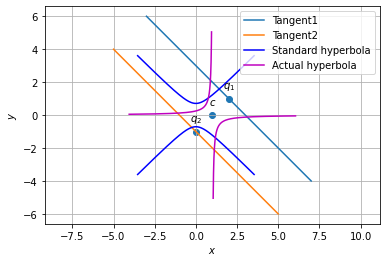
\includegraphics[width=\columnwidth]{./solutions/1/14/graph7.png}
	\caption{The standard and actual hyperbola.}
\end{figure}

\item \myvec{1\\2\\3}\myvec{2 &3 &4} 
\\
\solution 
The given curve 
\begin{align}
	y =\frac{1}{x-1}
\end{align}
can be expressed as 
\begin{align}
	xy - y - 1 = 0 \label{eq:solutions/1/14/eq:hyperbola}
\end{align}
Hence, we have
\begin{align}
	\vec{V} = \frac{1}{2}\myvec{0 & 1 \\ 1 & 0}, 
	\vec{u} = \frac{1}{2}\myvec{0 \\-1},
	f = -1
\end{align}
Since $\mydet{\vec{V}} < 0$, the equation \eqref{eq:solutions/1/14/eq:hyperbola} represents hyperbola.
To find the values of $\lambda_1$ and $\lambda_2$, consider the characteristic equation,
\begin{align}
	\mydet{\lambda\vec{I} - \vec{V}} &= 0\\
	\implies \mydet{\myvec{\lambda & 0\\0 & \lambda} - \myvec{0 & \frac{1}{2} \\ \frac{1}{2} & 0}} &= 0\\
	\implies \mydet{ \lambda & \frac{-1}{2} \\ \frac{-1}{2} & \lambda} &= 0\\
	\implies \lambda_1 &= \frac{1}{2} , \lambda_2 = \frac{-1}{2}
\end{align}
In addition, given the slope -1, the direction and normal vectors are given by 
\begin{align}
	\vec{m} = \myvec{1 \\ -1} \\
	\vec{n} = \myvec{ 1 \\ 1}
\end{align}
The parameters of hyperbola are as follows:
\begin{align}
	\vec{c} &= -\vec{V}^{-1}\vec{u} \\
	&= -\myvec{0 & 2\\ 2 & 0}\myvec{0 \\ -\frac{1}{2}} \\
	&= \myvec{1 \\ 0}\\
	axes &= \begin{cases}
	\sqrt{\frac{\vec{u}^T\vec{V}^{-1}\vec{u} - f}{\lambda_1}} = \sqrt{2}\\
 \sqrt{\frac{f-\vec{u}^T\vec{V}^{-1}\vec{u}}{\lambda_2}} = \sqrt{2}
\end{cases}
\end{align}
which represents the standard hyperbola equation,
\begin{align}
	\frac{x^2}{2} - \frac{x^2}{2} = 1
\end{align}
The points of contact are given by 
\begin{align}
  \tiny{K} &=\pm \sqrt{\frac{\vec{u}^T\vec{V}^{-1}\vec{u} - f}{\vec{n}^T\vec{V}^{-1}\vec{n}}}
  = \pm \frac{1}{2}\\
  \vec{q} &= \vec{V}^{-1}(k\vec{n}-\vec{u})\\
  \vec{q_1} &= \myvec{0 & 2\\2 & 0} \sbrak{\frac{1}{2}\myvec{1 \\ 1} - \myvec{0\\ \frac{-1}{2}}}\\
  &= \myvec{2 \\ 1}\\
  \vec{q_2} &= \myvec{0 & 2\\2 & 0} \sbrak{\frac{-1}{2}\myvec{1 \\ 1} - \myvec{0\\ \frac{-1}{2}}}\\
  &= \myvec{0 \\ -1}
\end{align} 
$\therefore$ The tangents are given by
\begin{align}
	\myvec{1 & 1} \brak{\vec{x} - \myvec{2 \\ 1}} = 0 \\
	\myvec{1 & 1} \brak{\vec{x} - \myvec{0 \\ -1}} = 0
\end{align}
The desired equations of all lines having slope -1 that are tangents to the curve $\frac{1}{x-1}, x \neq 1$ are given by
\begin{align}
	\myvec{1 & 1}\vec{x} &= 3 \\
	\myvec{1 & 1}\vec{x} &= -1 
\end{align}
The above results are verified in the following figure.
\begin{figure}[h!] \label{eq:solutions/1/14/fig:tangents}
	\centering
	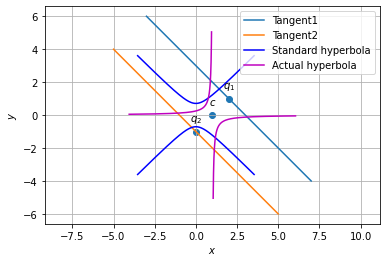
\includegraphics[width=\columnwidth]{./solutions/1/14/graph7.png}
	\caption{The standard and actual hyperbola.}
\end{figure}

\item \myvec{1 &-2\\2 &3}\myvec{1 &2 &3\\2 &3 &1} \\
\end{enumerate}
\item Simplify $\cos\theta$$\myvec{\cos\theta &\sin\theta\\ -\sin\theta &\cos\theta}$+$\sin\theta$$\myvec{\sin\theta &-\cos\theta\\ \cos\theta &\sin\theta}$\\
\solution 
The given curve 
\begin{align}
	y =\frac{1}{x-1}
\end{align}
can be expressed as 
\begin{align}
	xy - y - 1 = 0 \label{eq:solutions/1/14/eq:hyperbola}
\end{align}
Hence, we have
\begin{align}
	\vec{V} = \frac{1}{2}\myvec{0 & 1 \\ 1 & 0}, 
	\vec{u} = \frac{1}{2}\myvec{0 \\-1},
	f = -1
\end{align}
Since $\mydet{\vec{V}} < 0$, the equation \eqref{eq:solutions/1/14/eq:hyperbola} represents hyperbola.
To find the values of $\lambda_1$ and $\lambda_2$, consider the characteristic equation,
\begin{align}
	\mydet{\lambda\vec{I} - \vec{V}} &= 0\\
	\implies \mydet{\myvec{\lambda & 0\\0 & \lambda} - \myvec{0 & \frac{1}{2} \\ \frac{1}{2} & 0}} &= 0\\
	\implies \mydet{ \lambda & \frac{-1}{2} \\ \frac{-1}{2} & \lambda} &= 0\\
	\implies \lambda_1 &= \frac{1}{2} , \lambda_2 = \frac{-1}{2}
\end{align}
In addition, given the slope -1, the direction and normal vectors are given by 
\begin{align}
	\vec{m} = \myvec{1 \\ -1} \\
	\vec{n} = \myvec{ 1 \\ 1}
\end{align}
The parameters of hyperbola are as follows:
\begin{align}
	\vec{c} &= -\vec{V}^{-1}\vec{u} \\
	&= -\myvec{0 & 2\\ 2 & 0}\myvec{0 \\ -\frac{1}{2}} \\
	&= \myvec{1 \\ 0}\\
	axes &= \begin{cases}
	\sqrt{\frac{\vec{u}^T\vec{V}^{-1}\vec{u} - f}{\lambda_1}} = \sqrt{2}\\
 \sqrt{\frac{f-\vec{u}^T\vec{V}^{-1}\vec{u}}{\lambda_2}} = \sqrt{2}
\end{cases}
\end{align}
which represents the standard hyperbola equation,
\begin{align}
	\frac{x^2}{2} - \frac{x^2}{2} = 1
\end{align}
The points of contact are given by 
\begin{align}
  \tiny{K} &=\pm \sqrt{\frac{\vec{u}^T\vec{V}^{-1}\vec{u} - f}{\vec{n}^T\vec{V}^{-1}\vec{n}}}
  = \pm \frac{1}{2}\\
  \vec{q} &= \vec{V}^{-1}(k\vec{n}-\vec{u})\\
  \vec{q_1} &= \myvec{0 & 2\\2 & 0} \sbrak{\frac{1}{2}\myvec{1 \\ 1} - \myvec{0\\ \frac{-1}{2}}}\\
  &= \myvec{2 \\ 1}\\
  \vec{q_2} &= \myvec{0 & 2\\2 & 0} \sbrak{\frac{-1}{2}\myvec{1 \\ 1} - \myvec{0\\ \frac{-1}{2}}}\\
  &= \myvec{0 \\ -1}
\end{align} 
$\therefore$ The tangents are given by
\begin{align}
	\myvec{1 & 1} \brak{\vec{x} - \myvec{2 \\ 1}} = 0 \\
	\myvec{1 & 1} \brak{\vec{x} - \myvec{0 \\ -1}} = 0
\end{align}
The desired equations of all lines having slope -1 that are tangents to the curve $\frac{1}{x-1}, x \neq 1$ are given by
\begin{align}
	\myvec{1 & 1}\vec{x} &= 3 \\
	\myvec{1 & 1}\vec{x} &= -1 
\end{align}
The above results are verified in the following figure.
\begin{figure}[h!] \label{eq:solutions/1/14/fig:tangents}
	\centering
	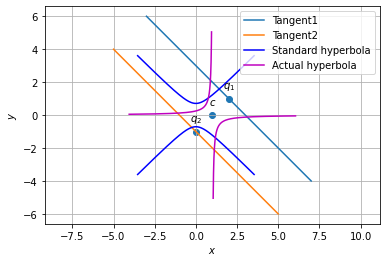
\includegraphics[width=\columnwidth]{./solutions/1/14/graph7.png}
	\caption{The standard and actual hyperbola.}
\end{figure}

\item Find X and Y,if\\
(i)X+Y=\myvec{7 &0\\2 &5} and X-Y=\myvec{3 &0\\0 &3}\\
(ii)2X+3Y=\myvec{2 &3\\4 &0} and 3X+2Y=\myvec{2 &-2\\-1 &5}\\ 
\solution 
The given curve 
\begin{align}
	y =\frac{1}{x-1}
\end{align}
can be expressed as 
\begin{align}
	xy - y - 1 = 0 \label{eq:solutions/1/14/eq:hyperbola}
\end{align}
Hence, we have
\begin{align}
	\vec{V} = \frac{1}{2}\myvec{0 & 1 \\ 1 & 0}, 
	\vec{u} = \frac{1}{2}\myvec{0 \\-1},
	f = -1
\end{align}
Since $\mydet{\vec{V}} < 0$, the equation \eqref{eq:solutions/1/14/eq:hyperbola} represents hyperbola.
To find the values of $\lambda_1$ and $\lambda_2$, consider the characteristic equation,
\begin{align}
	\mydet{\lambda\vec{I} - \vec{V}} &= 0\\
	\implies \mydet{\myvec{\lambda & 0\\0 & \lambda} - \myvec{0 & \frac{1}{2} \\ \frac{1}{2} & 0}} &= 0\\
	\implies \mydet{ \lambda & \frac{-1}{2} \\ \frac{-1}{2} & \lambda} &= 0\\
	\implies \lambda_1 &= \frac{1}{2} , \lambda_2 = \frac{-1}{2}
\end{align}
In addition, given the slope -1, the direction and normal vectors are given by 
\begin{align}
	\vec{m} = \myvec{1 \\ -1} \\
	\vec{n} = \myvec{ 1 \\ 1}
\end{align}
The parameters of hyperbola are as follows:
\begin{align}
	\vec{c} &= -\vec{V}^{-1}\vec{u} \\
	&= -\myvec{0 & 2\\ 2 & 0}\myvec{0 \\ -\frac{1}{2}} \\
	&= \myvec{1 \\ 0}\\
	axes &= \begin{cases}
	\sqrt{\frac{\vec{u}^T\vec{V}^{-1}\vec{u} - f}{\lambda_1}} = \sqrt{2}\\
 \sqrt{\frac{f-\vec{u}^T\vec{V}^{-1}\vec{u}}{\lambda_2}} = \sqrt{2}
\end{cases}
\end{align}
which represents the standard hyperbola equation,
\begin{align}
	\frac{x^2}{2} - \frac{x^2}{2} = 1
\end{align}
The points of contact are given by 
\begin{align}
  \tiny{K} &=\pm \sqrt{\frac{\vec{u}^T\vec{V}^{-1}\vec{u} - f}{\vec{n}^T\vec{V}^{-1}\vec{n}}}
  = \pm \frac{1}{2}\\
  \vec{q} &= \vec{V}^{-1}(k\vec{n}-\vec{u})\\
  \vec{q_1} &= \myvec{0 & 2\\2 & 0} \sbrak{\frac{1}{2}\myvec{1 \\ 1} - \myvec{0\\ \frac{-1}{2}}}\\
  &= \myvec{2 \\ 1}\\
  \vec{q_2} &= \myvec{0 & 2\\2 & 0} \sbrak{\frac{-1}{2}\myvec{1 \\ 1} - \myvec{0\\ \frac{-1}{2}}}\\
  &= \myvec{0 \\ -1}
\end{align} 
$\therefore$ The tangents are given by
\begin{align}
	\myvec{1 & 1} \brak{\vec{x} - \myvec{2 \\ 1}} = 0 \\
	\myvec{1 & 1} \brak{\vec{x} - \myvec{0 \\ -1}} = 0
\end{align}
The desired equations of all lines having slope -1 that are tangents to the curve $\frac{1}{x-1}, x \neq 1$ are given by
\begin{align}
	\myvec{1 & 1}\vec{x} &= 3 \\
	\myvec{1 & 1}\vec{x} &= -1 
\end{align}
The above results are verified in the following figure.
\begin{figure}[h!] \label{eq:solutions/1/14/fig:tangents}
	\centering
	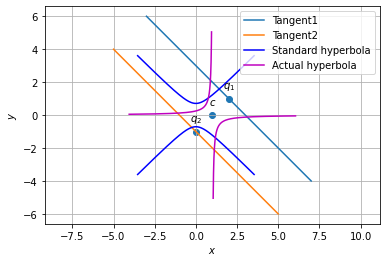
\includegraphics[width=\columnwidth]{./solutions/1/14/graph7.png}
	\caption{The standard and actual hyperbola.}
\end{figure}

\item Find X if Y=\myvec{3 &2\\1 &4} and 2X+Y=\myvec{1 &0\\-3 &2}\\
\solution 
The given curve 
\begin{align}
	y =\frac{1}{x-1}
\end{align}
can be expressed as 
\begin{align}
	xy - y - 1 = 0 \label{eq:solutions/1/14/eq:hyperbola}
\end{align}
Hence, we have
\begin{align}
	\vec{V} = \frac{1}{2}\myvec{0 & 1 \\ 1 & 0}, 
	\vec{u} = \frac{1}{2}\myvec{0 \\-1},
	f = -1
\end{align}
Since $\mydet{\vec{V}} < 0$, the equation \eqref{eq:solutions/1/14/eq:hyperbola} represents hyperbola.
To find the values of $\lambda_1$ and $\lambda_2$, consider the characteristic equation,
\begin{align}
	\mydet{\lambda\vec{I} - \vec{V}} &= 0\\
	\implies \mydet{\myvec{\lambda & 0\\0 & \lambda} - \myvec{0 & \frac{1}{2} \\ \frac{1}{2} & 0}} &= 0\\
	\implies \mydet{ \lambda & \frac{-1}{2} \\ \frac{-1}{2} & \lambda} &= 0\\
	\implies \lambda_1 &= \frac{1}{2} , \lambda_2 = \frac{-1}{2}
\end{align}
In addition, given the slope -1, the direction and normal vectors are given by 
\begin{align}
	\vec{m} = \myvec{1 \\ -1} \\
	\vec{n} = \myvec{ 1 \\ 1}
\end{align}
The parameters of hyperbola are as follows:
\begin{align}
	\vec{c} &= -\vec{V}^{-1}\vec{u} \\
	&= -\myvec{0 & 2\\ 2 & 0}\myvec{0 \\ -\frac{1}{2}} \\
	&= \myvec{1 \\ 0}\\
	axes &= \begin{cases}
	\sqrt{\frac{\vec{u}^T\vec{V}^{-1}\vec{u} - f}{\lambda_1}} = \sqrt{2}\\
 \sqrt{\frac{f-\vec{u}^T\vec{V}^{-1}\vec{u}}{\lambda_2}} = \sqrt{2}
\end{cases}
\end{align}
which represents the standard hyperbola equation,
\begin{align}
	\frac{x^2}{2} - \frac{x^2}{2} = 1
\end{align}
The points of contact are given by 
\begin{align}
  \tiny{K} &=\pm \sqrt{\frac{\vec{u}^T\vec{V}^{-1}\vec{u} - f}{\vec{n}^T\vec{V}^{-1}\vec{n}}}
  = \pm \frac{1}{2}\\
  \vec{q} &= \vec{V}^{-1}(k\vec{n}-\vec{u})\\
  \vec{q_1} &= \myvec{0 & 2\\2 & 0} \sbrak{\frac{1}{2}\myvec{1 \\ 1} - \myvec{0\\ \frac{-1}{2}}}\\
  &= \myvec{2 \\ 1}\\
  \vec{q_2} &= \myvec{0 & 2\\2 & 0} \sbrak{\frac{-1}{2}\myvec{1 \\ 1} - \myvec{0\\ \frac{-1}{2}}}\\
  &= \myvec{0 \\ -1}
\end{align} 
$\therefore$ The tangents are given by
\begin{align}
	\myvec{1 & 1} \brak{\vec{x} - \myvec{2 \\ 1}} = 0 \\
	\myvec{1 & 1} \brak{\vec{x} - \myvec{0 \\ -1}} = 0
\end{align}
The desired equations of all lines having slope -1 that are tangents to the curve $\frac{1}{x-1}, x \neq 1$ are given by
\begin{align}
	\myvec{1 & 1}\vec{x} &= 3 \\
	\myvec{1 & 1}\vec{x} &= -1 
\end{align}
The above results are verified in the following figure.
\begin{figure}[h!] \label{eq:solutions/1/14/fig:tangents}
	\centering
	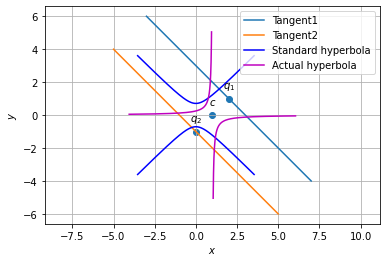
\includegraphics[width=\columnwidth]{./solutions/1/14/graph7.png}
	\caption{The standard and actual hyperbola.}
\end{figure}

\item If F(x)=$\myvec{\cos x &-\sin x &0\\ \sin x &\cos x &0\\0 &0 &1}$\\,show that F(x)F(y)=F(x+y)\\
\solution 
The given curve 
\begin{align}
	y =\frac{1}{x-1}
\end{align}
can be expressed as 
\begin{align}
	xy - y - 1 = 0 \label{eq:solutions/1/14/eq:hyperbola}
\end{align}
Hence, we have
\begin{align}
	\vec{V} = \frac{1}{2}\myvec{0 & 1 \\ 1 & 0}, 
	\vec{u} = \frac{1}{2}\myvec{0 \\-1},
	f = -1
\end{align}
Since $\mydet{\vec{V}} < 0$, the equation \eqref{eq:solutions/1/14/eq:hyperbola} represents hyperbola.
To find the values of $\lambda_1$ and $\lambda_2$, consider the characteristic equation,
\begin{align}
	\mydet{\lambda\vec{I} - \vec{V}} &= 0\\
	\implies \mydet{\myvec{\lambda & 0\\0 & \lambda} - \myvec{0 & \frac{1}{2} \\ \frac{1}{2} & 0}} &= 0\\
	\implies \mydet{ \lambda & \frac{-1}{2} \\ \frac{-1}{2} & \lambda} &= 0\\
	\implies \lambda_1 &= \frac{1}{2} , \lambda_2 = \frac{-1}{2}
\end{align}
In addition, given the slope -1, the direction and normal vectors are given by 
\begin{align}
	\vec{m} = \myvec{1 \\ -1} \\
	\vec{n} = \myvec{ 1 \\ 1}
\end{align}
The parameters of hyperbola are as follows:
\begin{align}
	\vec{c} &= -\vec{V}^{-1}\vec{u} \\
	&= -\myvec{0 & 2\\ 2 & 0}\myvec{0 \\ -\frac{1}{2}} \\
	&= \myvec{1 \\ 0}\\
	axes &= \begin{cases}
	\sqrt{\frac{\vec{u}^T\vec{V}^{-1}\vec{u} - f}{\lambda_1}} = \sqrt{2}\\
 \sqrt{\frac{f-\vec{u}^T\vec{V}^{-1}\vec{u}}{\lambda_2}} = \sqrt{2}
\end{cases}
\end{align}
which represents the standard hyperbola equation,
\begin{align}
	\frac{x^2}{2} - \frac{x^2}{2} = 1
\end{align}
The points of contact are given by 
\begin{align}
  \tiny{K} &=\pm \sqrt{\frac{\vec{u}^T\vec{V}^{-1}\vec{u} - f}{\vec{n}^T\vec{V}^{-1}\vec{n}}}
  = \pm \frac{1}{2}\\
  \vec{q} &= \vec{V}^{-1}(k\vec{n}-\vec{u})\\
  \vec{q_1} &= \myvec{0 & 2\\2 & 0} \sbrak{\frac{1}{2}\myvec{1 \\ 1} - \myvec{0\\ \frac{-1}{2}}}\\
  &= \myvec{2 \\ 1}\\
  \vec{q_2} &= \myvec{0 & 2\\2 & 0} \sbrak{\frac{-1}{2}\myvec{1 \\ 1} - \myvec{0\\ \frac{-1}{2}}}\\
  &= \myvec{0 \\ -1}
\end{align} 
$\therefore$ The tangents are given by
\begin{align}
	\myvec{1 & 1} \brak{\vec{x} - \myvec{2 \\ 1}} = 0 \\
	\myvec{1 & 1} \brak{\vec{x} - \myvec{0 \\ -1}} = 0
\end{align}
The desired equations of all lines having slope -1 that are tangents to the curve $\frac{1}{x-1}, x \neq 1$ are given by
\begin{align}
	\myvec{1 & 1}\vec{x} &= 3 \\
	\myvec{1 & 1}\vec{x} &= -1 
\end{align}
The above results are verified in the following figure.
\begin{figure}[h!] \label{eq:solutions/1/14/fig:tangents}
	\centering
	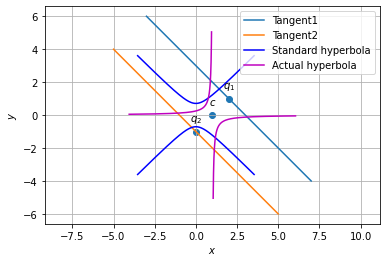
\includegraphics[width=\columnwidth]{./solutions/1/14/graph7.png}
	\caption{The standard and actual hyperbola.}
\end{figure}

\item Find $A^{2}-5A+6I$,if A = \myvec{2 &0 &1\\2 &1 &3\\1 &-1 &0}\\
\solution 
The given curve 
\begin{align}
	y =\frac{1}{x-1}
\end{align}
can be expressed as 
\begin{align}
	xy - y - 1 = 0 \label{eq:solutions/1/14/eq:hyperbola}
\end{align}
Hence, we have
\begin{align}
	\vec{V} = \frac{1}{2}\myvec{0 & 1 \\ 1 & 0}, 
	\vec{u} = \frac{1}{2}\myvec{0 \\-1},
	f = -1
\end{align}
Since $\mydet{\vec{V}} < 0$, the equation \eqref{eq:solutions/1/14/eq:hyperbola} represents hyperbola.
To find the values of $\lambda_1$ and $\lambda_2$, consider the characteristic equation,
\begin{align}
	\mydet{\lambda\vec{I} - \vec{V}} &= 0\\
	\implies \mydet{\myvec{\lambda & 0\\0 & \lambda} - \myvec{0 & \frac{1}{2} \\ \frac{1}{2} & 0}} &= 0\\
	\implies \mydet{ \lambda & \frac{-1}{2} \\ \frac{-1}{2} & \lambda} &= 0\\
	\implies \lambda_1 &= \frac{1}{2} , \lambda_2 = \frac{-1}{2}
\end{align}
In addition, given the slope -1, the direction and normal vectors are given by 
\begin{align}
	\vec{m} = \myvec{1 \\ -1} \\
	\vec{n} = \myvec{ 1 \\ 1}
\end{align}
The parameters of hyperbola are as follows:
\begin{align}
	\vec{c} &= -\vec{V}^{-1}\vec{u} \\
	&= -\myvec{0 & 2\\ 2 & 0}\myvec{0 \\ -\frac{1}{2}} \\
	&= \myvec{1 \\ 0}\\
	axes &= \begin{cases}
	\sqrt{\frac{\vec{u}^T\vec{V}^{-1}\vec{u} - f}{\lambda_1}} = \sqrt{2}\\
 \sqrt{\frac{f-\vec{u}^T\vec{V}^{-1}\vec{u}}{\lambda_2}} = \sqrt{2}
\end{cases}
\end{align}
which represents the standard hyperbola equation,
\begin{align}
	\frac{x^2}{2} - \frac{x^2}{2} = 1
\end{align}
The points of contact are given by 
\begin{align}
  \tiny{K} &=\pm \sqrt{\frac{\vec{u}^T\vec{V}^{-1}\vec{u} - f}{\vec{n}^T\vec{V}^{-1}\vec{n}}}
  = \pm \frac{1}{2}\\
  \vec{q} &= \vec{V}^{-1}(k\vec{n}-\vec{u})\\
  \vec{q_1} &= \myvec{0 & 2\\2 & 0} \sbrak{\frac{1}{2}\myvec{1 \\ 1} - \myvec{0\\ \frac{-1}{2}}}\\
  &= \myvec{2 \\ 1}\\
  \vec{q_2} &= \myvec{0 & 2\\2 & 0} \sbrak{\frac{-1}{2}\myvec{1 \\ 1} - \myvec{0\\ \frac{-1}{2}}}\\
  &= \myvec{0 \\ -1}
\end{align} 
$\therefore$ The tangents are given by
\begin{align}
	\myvec{1 & 1} \brak{\vec{x} - \myvec{2 \\ 1}} = 0 \\
	\myvec{1 & 1} \brak{\vec{x} - \myvec{0 \\ -1}} = 0
\end{align}
The desired equations of all lines having slope -1 that are tangents to the curve $\frac{1}{x-1}, x \neq 1$ are given by
\begin{align}
	\myvec{1 & 1}\vec{x} &= 3 \\
	\myvec{1 & 1}\vec{x} &= -1 
\end{align}
The above results are verified in the following figure.
\begin{figure}[h!] \label{eq:solutions/1/14/fig:tangents}
	\centering
	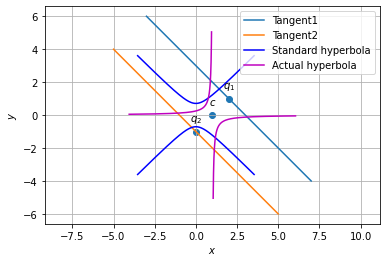
\includegraphics[width=\columnwidth]{./solutions/1/14/graph7.png}
	\caption{The standard and actual hyperbola.}
\end{figure}

\item If A=\myvec{1 &0 &2\\0 &2 &1\\2 &0 &3},prove that $A^3-6A^2+7A+2I=0$\\
\solution 
The given curve 
\begin{align}
	y =\frac{1}{x-1}
\end{align}
can be expressed as 
\begin{align}
	xy - y - 1 = 0 \label{eq:solutions/1/14/eq:hyperbola}
\end{align}
Hence, we have
\begin{align}
	\vec{V} = \frac{1}{2}\myvec{0 & 1 \\ 1 & 0}, 
	\vec{u} = \frac{1}{2}\myvec{0 \\-1},
	f = -1
\end{align}
Since $\mydet{\vec{V}} < 0$, the equation \eqref{eq:solutions/1/14/eq:hyperbola} represents hyperbola.
To find the values of $\lambda_1$ and $\lambda_2$, consider the characteristic equation,
\begin{align}
	\mydet{\lambda\vec{I} - \vec{V}} &= 0\\
	\implies \mydet{\myvec{\lambda & 0\\0 & \lambda} - \myvec{0 & \frac{1}{2} \\ \frac{1}{2} & 0}} &= 0\\
	\implies \mydet{ \lambda & \frac{-1}{2} \\ \frac{-1}{2} & \lambda} &= 0\\
	\implies \lambda_1 &= \frac{1}{2} , \lambda_2 = \frac{-1}{2}
\end{align}
In addition, given the slope -1, the direction and normal vectors are given by 
\begin{align}
	\vec{m} = \myvec{1 \\ -1} \\
	\vec{n} = \myvec{ 1 \\ 1}
\end{align}
The parameters of hyperbola are as follows:
\begin{align}
	\vec{c} &= -\vec{V}^{-1}\vec{u} \\
	&= -\myvec{0 & 2\\ 2 & 0}\myvec{0 \\ -\frac{1}{2}} \\
	&= \myvec{1 \\ 0}\\
	axes &= \begin{cases}
	\sqrt{\frac{\vec{u}^T\vec{V}^{-1}\vec{u} - f}{\lambda_1}} = \sqrt{2}\\
 \sqrt{\frac{f-\vec{u}^T\vec{V}^{-1}\vec{u}}{\lambda_2}} = \sqrt{2}
\end{cases}
\end{align}
which represents the standard hyperbola equation,
\begin{align}
	\frac{x^2}{2} - \frac{x^2}{2} = 1
\end{align}
The points of contact are given by 
\begin{align}
  \tiny{K} &=\pm \sqrt{\frac{\vec{u}^T\vec{V}^{-1}\vec{u} - f}{\vec{n}^T\vec{V}^{-1}\vec{n}}}
  = \pm \frac{1}{2}\\
  \vec{q} &= \vec{V}^{-1}(k\vec{n}-\vec{u})\\
  \vec{q_1} &= \myvec{0 & 2\\2 & 0} \sbrak{\frac{1}{2}\myvec{1 \\ 1} - \myvec{0\\ \frac{-1}{2}}}\\
  &= \myvec{2 \\ 1}\\
  \vec{q_2} &= \myvec{0 & 2\\2 & 0} \sbrak{\frac{-1}{2}\myvec{1 \\ 1} - \myvec{0\\ \frac{-1}{2}}}\\
  &= \myvec{0 \\ -1}
\end{align} 
$\therefore$ The tangents are given by
\begin{align}
	\myvec{1 & 1} \brak{\vec{x} - \myvec{2 \\ 1}} = 0 \\
	\myvec{1 & 1} \brak{\vec{x} - \myvec{0 \\ -1}} = 0
\end{align}
The desired equations of all lines having slope -1 that are tangents to the curve $\frac{1}{x-1}, x \neq 1$ are given by
\begin{align}
	\myvec{1 & 1}\vec{x} &= 3 \\
	\myvec{1 & 1}\vec{x} &= -1 
\end{align}
The above results are verified in the following figure.
\begin{figure}[h!] \label{eq:solutions/1/14/fig:tangents}
	\centering
	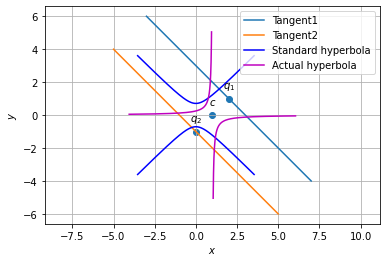
\includegraphics[width=\columnwidth]{./solutions/1/14/graph7.png}
	\caption{The standard and actual hyperbola.}
\end{figure}

\item If A=$\myvec{0 &-\tan\frac{\alpha}{2}\\  \tan\frac{\alpha}{2} &0}$ and I is the identity matrix of order 2,show that \\I+A=(I-A)$\myvec{\cos\alpha &-\sin\alpha\\\sin\alpha &\cos\alpha}$\\
\solution 
The given curve 
\begin{align}
	y =\frac{1}{x-1}
\end{align}
can be expressed as 
\begin{align}
	xy - y - 1 = 0 \label{eq:solutions/1/14/eq:hyperbola}
\end{align}
Hence, we have
\begin{align}
	\vec{V} = \frac{1}{2}\myvec{0 & 1 \\ 1 & 0}, 
	\vec{u} = \frac{1}{2}\myvec{0 \\-1},
	f = -1
\end{align}
Since $\mydet{\vec{V}} < 0$, the equation \eqref{eq:solutions/1/14/eq:hyperbola} represents hyperbola.
To find the values of $\lambda_1$ and $\lambda_2$, consider the characteristic equation,
\begin{align}
	\mydet{\lambda\vec{I} - \vec{V}} &= 0\\
	\implies \mydet{\myvec{\lambda & 0\\0 & \lambda} - \myvec{0 & \frac{1}{2} \\ \frac{1}{2} & 0}} &= 0\\
	\implies \mydet{ \lambda & \frac{-1}{2} \\ \frac{-1}{2} & \lambda} &= 0\\
	\implies \lambda_1 &= \frac{1}{2} , \lambda_2 = \frac{-1}{2}
\end{align}
In addition, given the slope -1, the direction and normal vectors are given by 
\begin{align}
	\vec{m} = \myvec{1 \\ -1} \\
	\vec{n} = \myvec{ 1 \\ 1}
\end{align}
The parameters of hyperbola are as follows:
\begin{align}
	\vec{c} &= -\vec{V}^{-1}\vec{u} \\
	&= -\myvec{0 & 2\\ 2 & 0}\myvec{0 \\ -\frac{1}{2}} \\
	&= \myvec{1 \\ 0}\\
	axes &= \begin{cases}
	\sqrt{\frac{\vec{u}^T\vec{V}^{-1}\vec{u} - f}{\lambda_1}} = \sqrt{2}\\
 \sqrt{\frac{f-\vec{u}^T\vec{V}^{-1}\vec{u}}{\lambda_2}} = \sqrt{2}
\end{cases}
\end{align}
which represents the standard hyperbola equation,
\begin{align}
	\frac{x^2}{2} - \frac{x^2}{2} = 1
\end{align}
The points of contact are given by 
\begin{align}
  \tiny{K} &=\pm \sqrt{\frac{\vec{u}^T\vec{V}^{-1}\vec{u} - f}{\vec{n}^T\vec{V}^{-1}\vec{n}}}
  = \pm \frac{1}{2}\\
  \vec{q} &= \vec{V}^{-1}(k\vec{n}-\vec{u})\\
  \vec{q_1} &= \myvec{0 & 2\\2 & 0} \sbrak{\frac{1}{2}\myvec{1 \\ 1} - \myvec{0\\ \frac{-1}{2}}}\\
  &= \myvec{2 \\ 1}\\
  \vec{q_2} &= \myvec{0 & 2\\2 & 0} \sbrak{\frac{-1}{2}\myvec{1 \\ 1} - \myvec{0\\ \frac{-1}{2}}}\\
  &= \myvec{0 \\ -1}
\end{align} 
$\therefore$ The tangents are given by
\begin{align}
	\myvec{1 & 1} \brak{\vec{x} - \myvec{2 \\ 1}} = 0 \\
	\myvec{1 & 1} \brak{\vec{x} - \myvec{0 \\ -1}} = 0
\end{align}
The desired equations of all lines having slope -1 that are tangents to the curve $\frac{1}{x-1}, x \neq 1$ are given by
\begin{align}
	\myvec{1 & 1}\vec{x} &= 3 \\
	\myvec{1 & 1}\vec{x} &= -1 
\end{align}
The above results are verified in the following figure.
\begin{figure}[h!] \label{eq:solutions/1/14/fig:tangents}
	\centering
	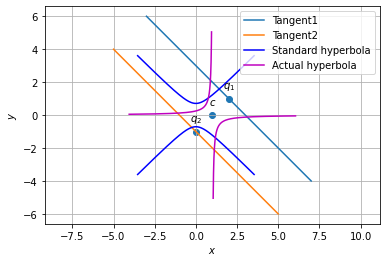
\includegraphics[width=\columnwidth]{./solutions/1/14/graph7.png}
	\caption{The standard and actual hyperbola.}
\end{figure}

\item A trust fund has \rupee{30,000} that must be invested in two different types of bonds.
The first bond pays 5\% interest per year, and the second bond pays 7\% interest
per year. Using matrix multiplication, determine how to divide \rupee{ 30,000} among
the two types of bonds. If the trust fund must obtain an annual total interest of:\\
(a) \rupee{1800} (b)\rupee{2000}\\
\solution 
The given curve 
\begin{align}
	y =\frac{1}{x-1}
\end{align}
can be expressed as 
\begin{align}
	xy - y - 1 = 0 \label{eq:solutions/1/14/eq:hyperbola}
\end{align}
Hence, we have
\begin{align}
	\vec{V} = \frac{1}{2}\myvec{0 & 1 \\ 1 & 0}, 
	\vec{u} = \frac{1}{2}\myvec{0 \\-1},
	f = -1
\end{align}
Since $\mydet{\vec{V}} < 0$, the equation \eqref{eq:solutions/1/14/eq:hyperbola} represents hyperbola.
To find the values of $\lambda_1$ and $\lambda_2$, consider the characteristic equation,
\begin{align}
	\mydet{\lambda\vec{I} - \vec{V}} &= 0\\
	\implies \mydet{\myvec{\lambda & 0\\0 & \lambda} - \myvec{0 & \frac{1}{2} \\ \frac{1}{2} & 0}} &= 0\\
	\implies \mydet{ \lambda & \frac{-1}{2} \\ \frac{-1}{2} & \lambda} &= 0\\
	\implies \lambda_1 &= \frac{1}{2} , \lambda_2 = \frac{-1}{2}
\end{align}
In addition, given the slope -1, the direction and normal vectors are given by 
\begin{align}
	\vec{m} = \myvec{1 \\ -1} \\
	\vec{n} = \myvec{ 1 \\ 1}
\end{align}
The parameters of hyperbola are as follows:
\begin{align}
	\vec{c} &= -\vec{V}^{-1}\vec{u} \\
	&= -\myvec{0 & 2\\ 2 & 0}\myvec{0 \\ -\frac{1}{2}} \\
	&= \myvec{1 \\ 0}\\
	axes &= \begin{cases}
	\sqrt{\frac{\vec{u}^T\vec{V}^{-1}\vec{u} - f}{\lambda_1}} = \sqrt{2}\\
 \sqrt{\frac{f-\vec{u}^T\vec{V}^{-1}\vec{u}}{\lambda_2}} = \sqrt{2}
\end{cases}
\end{align}
which represents the standard hyperbola equation,
\begin{align}
	\frac{x^2}{2} - \frac{x^2}{2} = 1
\end{align}
The points of contact are given by 
\begin{align}
  \tiny{K} &=\pm \sqrt{\frac{\vec{u}^T\vec{V}^{-1}\vec{u} - f}{\vec{n}^T\vec{V}^{-1}\vec{n}}}
  = \pm \frac{1}{2}\\
  \vec{q} &= \vec{V}^{-1}(k\vec{n}-\vec{u})\\
  \vec{q_1} &= \myvec{0 & 2\\2 & 0} \sbrak{\frac{1}{2}\myvec{1 \\ 1} - \myvec{0\\ \frac{-1}{2}}}\\
  &= \myvec{2 \\ 1}\\
  \vec{q_2} &= \myvec{0 & 2\\2 & 0} \sbrak{\frac{-1}{2}\myvec{1 \\ 1} - \myvec{0\\ \frac{-1}{2}}}\\
  &= \myvec{0 \\ -1}
\end{align} 
$\therefore$ The tangents are given by
\begin{align}
	\myvec{1 & 1} \brak{\vec{x} - \myvec{2 \\ 1}} = 0 \\
	\myvec{1 & 1} \brak{\vec{x} - \myvec{0 \\ -1}} = 0
\end{align}
The desired equations of all lines having slope -1 that are tangents to the curve $\frac{1}{x-1}, x \neq 1$ are given by
\begin{align}
	\myvec{1 & 1}\vec{x} &= 3 \\
	\myvec{1 & 1}\vec{x} &= -1 
\end{align}
The above results are verified in the following figure.
\begin{figure}[h!] \label{eq:solutions/1/14/fig:tangents}
	\centering
	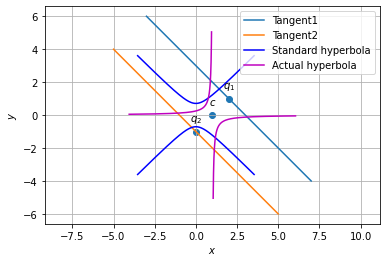
\includegraphics[width=\columnwidth]{./solutions/1/14/graph7.png}
	\caption{The standard and actual hyperbola.}
\end{figure}

\item For the matrices A and B,verify that $(AB)^{'}$=$B^{'}A^{'}$,where\\
(i)A=\myvec{1\\-4\\3},B=\myvec{-1 &2 &1} (ii)A=\myvec{0\\1\\2},B=\myvec{1 &5 &7}
\item If (i)  A=$\myvec{\cos\alpha &\sin\alpha\\-\sin\alpha &\cos\alpha}$, then verify that $A^{'}A=I$\\
        (ii) If A=$\myvec{\sin\alpha &\cos\alpha\\-\cos\alpha &\sin\alpha}$,then verify that $A^{'}A=I$\\
\solution
The given curve 
\begin{align}
	y =\frac{1}{x-1}
\end{align}
can be expressed as 
\begin{align}
	xy - y - 1 = 0 \label{eq:solutions/1/14/eq:hyperbola}
\end{align}
Hence, we have
\begin{align}
	\vec{V} = \frac{1}{2}\myvec{0 & 1 \\ 1 & 0}, 
	\vec{u} = \frac{1}{2}\myvec{0 \\-1},
	f = -1
\end{align}
Since $\mydet{\vec{V}} < 0$, the equation \eqref{eq:solutions/1/14/eq:hyperbola} represents hyperbola.
To find the values of $\lambda_1$ and $\lambda_2$, consider the characteristic equation,
\begin{align}
	\mydet{\lambda\vec{I} - \vec{V}} &= 0\\
	\implies \mydet{\myvec{\lambda & 0\\0 & \lambda} - \myvec{0 & \frac{1}{2} \\ \frac{1}{2} & 0}} &= 0\\
	\implies \mydet{ \lambda & \frac{-1}{2} \\ \frac{-1}{2} & \lambda} &= 0\\
	\implies \lambda_1 &= \frac{1}{2} , \lambda_2 = \frac{-1}{2}
\end{align}
In addition, given the slope -1, the direction and normal vectors are given by 
\begin{align}
	\vec{m} = \myvec{1 \\ -1} \\
	\vec{n} = \myvec{ 1 \\ 1}
\end{align}
The parameters of hyperbola are as follows:
\begin{align}
	\vec{c} &= -\vec{V}^{-1}\vec{u} \\
	&= -\myvec{0 & 2\\ 2 & 0}\myvec{0 \\ -\frac{1}{2}} \\
	&= \myvec{1 \\ 0}\\
	axes &= \begin{cases}
	\sqrt{\frac{\vec{u}^T\vec{V}^{-1}\vec{u} - f}{\lambda_1}} = \sqrt{2}\\
 \sqrt{\frac{f-\vec{u}^T\vec{V}^{-1}\vec{u}}{\lambda_2}} = \sqrt{2}
\end{cases}
\end{align}
which represents the standard hyperbola equation,
\begin{align}
	\frac{x^2}{2} - \frac{x^2}{2} = 1
\end{align}
The points of contact are given by 
\begin{align}
  \tiny{K} &=\pm \sqrt{\frac{\vec{u}^T\vec{V}^{-1}\vec{u} - f}{\vec{n}^T\vec{V}^{-1}\vec{n}}}
  = \pm \frac{1}{2}\\
  \vec{q} &= \vec{V}^{-1}(k\vec{n}-\vec{u})\\
  \vec{q_1} &= \myvec{0 & 2\\2 & 0} \sbrak{\frac{1}{2}\myvec{1 \\ 1} - \myvec{0\\ \frac{-1}{2}}}\\
  &= \myvec{2 \\ 1}\\
  \vec{q_2} &= \myvec{0 & 2\\2 & 0} \sbrak{\frac{-1}{2}\myvec{1 \\ 1} - \myvec{0\\ \frac{-1}{2}}}\\
  &= \myvec{0 \\ -1}
\end{align} 
$\therefore$ The tangents are given by
\begin{align}
	\myvec{1 & 1} \brak{\vec{x} - \myvec{2 \\ 1}} = 0 \\
	\myvec{1 & 1} \brak{\vec{x} - \myvec{0 \\ -1}} = 0
\end{align}
The desired equations of all lines having slope -1 that are tangents to the curve $\frac{1}{x-1}, x \neq 1$ are given by
\begin{align}
	\myvec{1 & 1}\vec{x} &= 3 \\
	\myvec{1 & 1}\vec{x} &= -1 
\end{align}
The above results are verified in the following figure.
\begin{figure}[h!] \label{eq:solutions/1/14/fig:tangents}
	\centering
	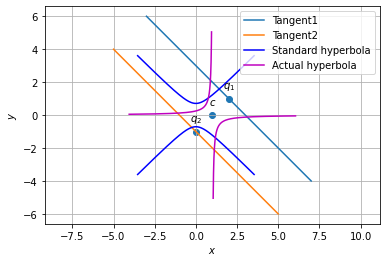
\includegraphics[width=\columnwidth]{./solutions/1/14/graph7.png}
	\caption{The standard and actual hyperbola.}
\end{figure}

  \item If A=$\myvec{\cos\alpha &-\sin\alpha\\ \sin\alpha &\cos\alpha}$,and $A+A^{'}=I$,then the value of $\alpha$ is\\
  (A) $\frac{\pi}{6}$\\ (B)$\frac{\pi}{3}$ \\
  (C) $\pi$ \\ (D)$\frac{3\pi}{2}$\\
\solution 
The given curve 
\begin{align}
	y =\frac{1}{x-1}
\end{align}
can be expressed as 
\begin{align}
	xy - y - 1 = 0 \label{eq:solutions/1/14/eq:hyperbola}
\end{align}
Hence, we have
\begin{align}
	\vec{V} = \frac{1}{2}\myvec{0 & 1 \\ 1 & 0}, 
	\vec{u} = \frac{1}{2}\myvec{0 \\-1},
	f = -1
\end{align}
Since $\mydet{\vec{V}} < 0$, the equation \eqref{eq:solutions/1/14/eq:hyperbola} represents hyperbola.
To find the values of $\lambda_1$ and $\lambda_2$, consider the characteristic equation,
\begin{align}
	\mydet{\lambda\vec{I} - \vec{V}} &= 0\\
	\implies \mydet{\myvec{\lambda & 0\\0 & \lambda} - \myvec{0 & \frac{1}{2} \\ \frac{1}{2} & 0}} &= 0\\
	\implies \mydet{ \lambda & \frac{-1}{2} \\ \frac{-1}{2} & \lambda} &= 0\\
	\implies \lambda_1 &= \frac{1}{2} , \lambda_2 = \frac{-1}{2}
\end{align}
In addition, given the slope -1, the direction and normal vectors are given by 
\begin{align}
	\vec{m} = \myvec{1 \\ -1} \\
	\vec{n} = \myvec{ 1 \\ 1}
\end{align}
The parameters of hyperbola are as follows:
\begin{align}
	\vec{c} &= -\vec{V}^{-1}\vec{u} \\
	&= -\myvec{0 & 2\\ 2 & 0}\myvec{0 \\ -\frac{1}{2}} \\
	&= \myvec{1 \\ 0}\\
	axes &= \begin{cases}
	\sqrt{\frac{\vec{u}^T\vec{V}^{-1}\vec{u} - f}{\lambda_1}} = \sqrt{2}\\
 \sqrt{\frac{f-\vec{u}^T\vec{V}^{-1}\vec{u}}{\lambda_2}} = \sqrt{2}
\end{cases}
\end{align}
which represents the standard hyperbola equation,
\begin{align}
	\frac{x^2}{2} - \frac{x^2}{2} = 1
\end{align}
The points of contact are given by 
\begin{align}
  \tiny{K} &=\pm \sqrt{\frac{\vec{u}^T\vec{V}^{-1}\vec{u} - f}{\vec{n}^T\vec{V}^{-1}\vec{n}}}
  = \pm \frac{1}{2}\\
  \vec{q} &= \vec{V}^{-1}(k\vec{n}-\vec{u})\\
  \vec{q_1} &= \myvec{0 & 2\\2 & 0} \sbrak{\frac{1}{2}\myvec{1 \\ 1} - \myvec{0\\ \frac{-1}{2}}}\\
  &= \myvec{2 \\ 1}\\
  \vec{q_2} &= \myvec{0 & 2\\2 & 0} \sbrak{\frac{-1}{2}\myvec{1 \\ 1} - \myvec{0\\ \frac{-1}{2}}}\\
  &= \myvec{0 \\ -1}
\end{align} 
$\therefore$ The tangents are given by
\begin{align}
	\myvec{1 & 1} \brak{\vec{x} - \myvec{2 \\ 1}} = 0 \\
	\myvec{1 & 1} \brak{\vec{x} - \myvec{0 \\ -1}} = 0
\end{align}
The desired equations of all lines having slope -1 that are tangents to the curve $\frac{1}{x-1}, x \neq 1$ are given by
\begin{align}
	\myvec{1 & 1}\vec{x} &= 3 \\
	\myvec{1 & 1}\vec{x} &= -1 
\end{align}
The above results are verified in the following figure.
\begin{figure}[h!] \label{eq:solutions/1/14/fig:tangents}
	\centering
	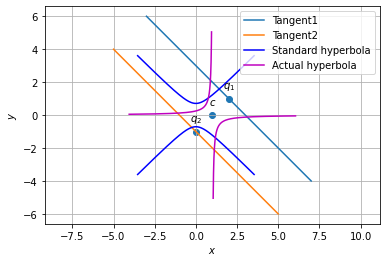
\includegraphics[width=\columnwidth]{./solutions/1/14/graph7.png}
	\caption{The standard and actual hyperbola.}
\end{figure}

  \item \myvec{2 &-3 &3\\2 &2 &3\\3 &-2 &2}\\
\solution
The given curve 
\begin{align}
	y =\frac{1}{x-1}
\end{align}
can be expressed as 
\begin{align}
	xy - y - 1 = 0 \label{eq:solutions/1/14/eq:hyperbola}
\end{align}
Hence, we have
\begin{align}
	\vec{V} = \frac{1}{2}\myvec{0 & 1 \\ 1 & 0}, 
	\vec{u} = \frac{1}{2}\myvec{0 \\-1},
	f = -1
\end{align}
Since $\mydet{\vec{V}} < 0$, the equation \eqref{eq:solutions/1/14/eq:hyperbola} represents hyperbola.
To find the values of $\lambda_1$ and $\lambda_2$, consider the characteristic equation,
\begin{align}
	\mydet{\lambda\vec{I} - \vec{V}} &= 0\\
	\implies \mydet{\myvec{\lambda & 0\\0 & \lambda} - \myvec{0 & \frac{1}{2} \\ \frac{1}{2} & 0}} &= 0\\
	\implies \mydet{ \lambda & \frac{-1}{2} \\ \frac{-1}{2} & \lambda} &= 0\\
	\implies \lambda_1 &= \frac{1}{2} , \lambda_2 = \frac{-1}{2}
\end{align}
In addition, given the slope -1, the direction and normal vectors are given by 
\begin{align}
	\vec{m} = \myvec{1 \\ -1} \\
	\vec{n} = \myvec{ 1 \\ 1}
\end{align}
The parameters of hyperbola are as follows:
\begin{align}
	\vec{c} &= -\vec{V}^{-1}\vec{u} \\
	&= -\myvec{0 & 2\\ 2 & 0}\myvec{0 \\ -\frac{1}{2}} \\
	&= \myvec{1 \\ 0}\\
	axes &= \begin{cases}
	\sqrt{\frac{\vec{u}^T\vec{V}^{-1}\vec{u} - f}{\lambda_1}} = \sqrt{2}\\
 \sqrt{\frac{f-\vec{u}^T\vec{V}^{-1}\vec{u}}{\lambda_2}} = \sqrt{2}
\end{cases}
\end{align}
which represents the standard hyperbola equation,
\begin{align}
	\frac{x^2}{2} - \frac{x^2}{2} = 1
\end{align}
The points of contact are given by 
\begin{align}
  \tiny{K} &=\pm \sqrt{\frac{\vec{u}^T\vec{V}^{-1}\vec{u} - f}{\vec{n}^T\vec{V}^{-1}\vec{n}}}
  = \pm \frac{1}{2}\\
  \vec{q} &= \vec{V}^{-1}(k\vec{n}-\vec{u})\\
  \vec{q_1} &= \myvec{0 & 2\\2 & 0} \sbrak{\frac{1}{2}\myvec{1 \\ 1} - \myvec{0\\ \frac{-1}{2}}}\\
  &= \myvec{2 \\ 1}\\
  \vec{q_2} &= \myvec{0 & 2\\2 & 0} \sbrak{\frac{-1}{2}\myvec{1 \\ 1} - \myvec{0\\ \frac{-1}{2}}}\\
  &= \myvec{0 \\ -1}
\end{align} 
$\therefore$ The tangents are given by
\begin{align}
	\myvec{1 & 1} \brak{\vec{x} - \myvec{2 \\ 1}} = 0 \\
	\myvec{1 & 1} \brak{\vec{x} - \myvec{0 \\ -1}} = 0
\end{align}
The desired equations of all lines having slope -1 that are tangents to the curve $\frac{1}{x-1}, x \neq 1$ are given by
\begin{align}
	\myvec{1 & 1}\vec{x} &= 3 \\
	\myvec{1 & 1}\vec{x} &= -1 
\end{align}
The above results are verified in the following figure.
\begin{figure}[h!] \label{eq:solutions/1/14/fig:tangents}
	\centering
	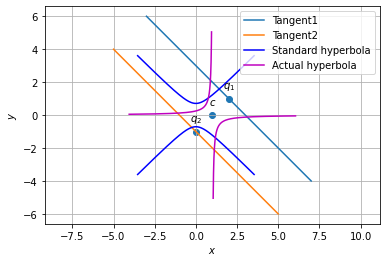
\includegraphics[width=\columnwidth]{./solutions/1/14/graph7.png}
	\caption{The standard and actual hyperbola.}
\end{figure}

  \item \myvec{1 &3 &-2\\-3 &0 &-5\\2 &5 &0}\\
\solution
The given curve 
\begin{align}
	y =\frac{1}{x-1}
\end{align}
can be expressed as 
\begin{align}
	xy - y - 1 = 0 \label{eq:solutions/1/14/eq:hyperbola}
\end{align}
Hence, we have
\begin{align}
	\vec{V} = \frac{1}{2}\myvec{0 & 1 \\ 1 & 0}, 
	\vec{u} = \frac{1}{2}\myvec{0 \\-1},
	f = -1
\end{align}
Since $\mydet{\vec{V}} < 0$, the equation \eqref{eq:solutions/1/14/eq:hyperbola} represents hyperbola.
To find the values of $\lambda_1$ and $\lambda_2$, consider the characteristic equation,
\begin{align}
	\mydet{\lambda\vec{I} - \vec{V}} &= 0\\
	\implies \mydet{\myvec{\lambda & 0\\0 & \lambda} - \myvec{0 & \frac{1}{2} \\ \frac{1}{2} & 0}} &= 0\\
	\implies \mydet{ \lambda & \frac{-1}{2} \\ \frac{-1}{2} & \lambda} &= 0\\
	\implies \lambda_1 &= \frac{1}{2} , \lambda_2 = \frac{-1}{2}
\end{align}
In addition, given the slope -1, the direction and normal vectors are given by 
\begin{align}
	\vec{m} = \myvec{1 \\ -1} \\
	\vec{n} = \myvec{ 1 \\ 1}
\end{align}
The parameters of hyperbola are as follows:
\begin{align}
	\vec{c} &= -\vec{V}^{-1}\vec{u} \\
	&= -\myvec{0 & 2\\ 2 & 0}\myvec{0 \\ -\frac{1}{2}} \\
	&= \myvec{1 \\ 0}\\
	axes &= \begin{cases}
	\sqrt{\frac{\vec{u}^T\vec{V}^{-1}\vec{u} - f}{\lambda_1}} = \sqrt{2}\\
 \sqrt{\frac{f-\vec{u}^T\vec{V}^{-1}\vec{u}}{\lambda_2}} = \sqrt{2}
\end{cases}
\end{align}
which represents the standard hyperbola equation,
\begin{align}
	\frac{x^2}{2} - \frac{x^2}{2} = 1
\end{align}
The points of contact are given by 
\begin{align}
  \tiny{K} &=\pm \sqrt{\frac{\vec{u}^T\vec{V}^{-1}\vec{u} - f}{\vec{n}^T\vec{V}^{-1}\vec{n}}}
  = \pm \frac{1}{2}\\
  \vec{q} &= \vec{V}^{-1}(k\vec{n}-\vec{u})\\
  \vec{q_1} &= \myvec{0 & 2\\2 & 0} \sbrak{\frac{1}{2}\myvec{1 \\ 1} - \myvec{0\\ \frac{-1}{2}}}\\
  &= \myvec{2 \\ 1}\\
  \vec{q_2} &= \myvec{0 & 2\\2 & 0} \sbrak{\frac{-1}{2}\myvec{1 \\ 1} - \myvec{0\\ \frac{-1}{2}}}\\
  &= \myvec{0 \\ -1}
\end{align} 
$\therefore$ The tangents are given by
\begin{align}
	\myvec{1 & 1} \brak{\vec{x} - \myvec{2 \\ 1}} = 0 \\
	\myvec{1 & 1} \brak{\vec{x} - \myvec{0 \\ -1}} = 0
\end{align}
The desired equations of all lines having slope -1 that are tangents to the curve $\frac{1}{x-1}, x \neq 1$ are given by
\begin{align}
	\myvec{1 & 1}\vec{x} &= 3 \\
	\myvec{1 & 1}\vec{x} &= -1 
\end{align}
The above results are verified in the following figure.
\begin{figure}[h!] \label{eq:solutions/1/14/fig:tangents}
	\centering
	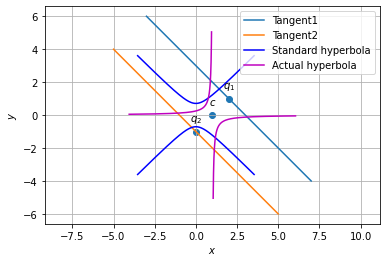
\includegraphics[width=\columnwidth]{./solutions/1/14/graph7.png}
	\caption{The standard and actual hyperbola.}
\end{figure}

  \item \myvec{2 &0 &-1\\5 &1 &0\\0 &1 &3}\\
\solution
The given curve 
\begin{align}
	y =\frac{1}{x-1}
\end{align}
can be expressed as 
\begin{align}
	xy - y - 1 = 0 \label{eq:solutions/1/14/eq:hyperbola}
\end{align}
Hence, we have
\begin{align}
	\vec{V} = \frac{1}{2}\myvec{0 & 1 \\ 1 & 0}, 
	\vec{u} = \frac{1}{2}\myvec{0 \\-1},
	f = -1
\end{align}
Since $\mydet{\vec{V}} < 0$, the equation \eqref{eq:solutions/1/14/eq:hyperbola} represents hyperbola.
To find the values of $\lambda_1$ and $\lambda_2$, consider the characteristic equation,
\begin{align}
	\mydet{\lambda\vec{I} - \vec{V}} &= 0\\
	\implies \mydet{\myvec{\lambda & 0\\0 & \lambda} - \myvec{0 & \frac{1}{2} \\ \frac{1}{2} & 0}} &= 0\\
	\implies \mydet{ \lambda & \frac{-1}{2} \\ \frac{-1}{2} & \lambda} &= 0\\
	\implies \lambda_1 &= \frac{1}{2} , \lambda_2 = \frac{-1}{2}
\end{align}
In addition, given the slope -1, the direction and normal vectors are given by 
\begin{align}
	\vec{m} = \myvec{1 \\ -1} \\
	\vec{n} = \myvec{ 1 \\ 1}
\end{align}
The parameters of hyperbola are as follows:
\begin{align}
	\vec{c} &= -\vec{V}^{-1}\vec{u} \\
	&= -\myvec{0 & 2\\ 2 & 0}\myvec{0 \\ -\frac{1}{2}} \\
	&= \myvec{1 \\ 0}\\
	axes &= \begin{cases}
	\sqrt{\frac{\vec{u}^T\vec{V}^{-1}\vec{u} - f}{\lambda_1}} = \sqrt{2}\\
 \sqrt{\frac{f-\vec{u}^T\vec{V}^{-1}\vec{u}}{\lambda_2}} = \sqrt{2}
\end{cases}
\end{align}
which represents the standard hyperbola equation,
\begin{align}
	\frac{x^2}{2} - \frac{x^2}{2} = 1
\end{align}
The points of contact are given by 
\begin{align}
  \tiny{K} &=\pm \sqrt{\frac{\vec{u}^T\vec{V}^{-1}\vec{u} - f}{\vec{n}^T\vec{V}^{-1}\vec{n}}}
  = \pm \frac{1}{2}\\
  \vec{q} &= \vec{V}^{-1}(k\vec{n}-\vec{u})\\
  \vec{q_1} &= \myvec{0 & 2\\2 & 0} \sbrak{\frac{1}{2}\myvec{1 \\ 1} - \myvec{0\\ \frac{-1}{2}}}\\
  &= \myvec{2 \\ 1}\\
  \vec{q_2} &= \myvec{0 & 2\\2 & 0} \sbrak{\frac{-1}{2}\myvec{1 \\ 1} - \myvec{0\\ \frac{-1}{2}}}\\
  &= \myvec{0 \\ -1}
\end{align} 
$\therefore$ The tangents are given by
\begin{align}
	\myvec{1 & 1} \brak{\vec{x} - \myvec{2 \\ 1}} = 0 \\
	\myvec{1 & 1} \brak{\vec{x} - \myvec{0 \\ -1}} = 0
\end{align}
The desired equations of all lines having slope -1 that are tangents to the curve $\frac{1}{x-1}, x \neq 1$ are given by
\begin{align}
	\myvec{1 & 1}\vec{x} &= 3 \\
	\myvec{1 & 1}\vec{x} &= -1 
\end{align}
The above results are verified in the following figure.
\begin{figure}[h!] \label{eq:solutions/1/14/fig:tangents}
	\centering
	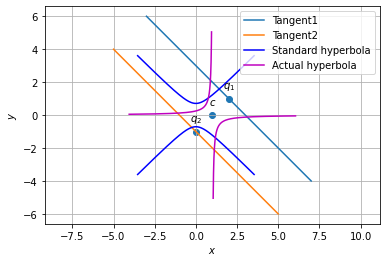
\includegraphics[width=\columnwidth]{./solutions/1/14/graph7.png}
	\caption{The standard and actual hyperbola.}
\end{figure}

  \item If A=\myvec{1 &1 &1\\1 &1 &1\\1 &1 &1},\\prove that $A^{n}$=$\myvec{3^{n-1} &3^{n-1}&3^{n-1}\\3^{n-1}&3^{n-1}&3^{n-1}\\3^{n-1}&3^{n-1} &3^{n-1}}$,$n \epsilon N$\\
\solution
The given curve 
\begin{align}
	y =\frac{1}{x-1}
\end{align}
can be expressed as 
\begin{align}
	xy - y - 1 = 0 \label{eq:solutions/1/14/eq:hyperbola}
\end{align}
Hence, we have
\begin{align}
	\vec{V} = \frac{1}{2}\myvec{0 & 1 \\ 1 & 0}, 
	\vec{u} = \frac{1}{2}\myvec{0 \\-1},
	f = -1
\end{align}
Since $\mydet{\vec{V}} < 0$, the equation \eqref{eq:solutions/1/14/eq:hyperbola} represents hyperbola.
To find the values of $\lambda_1$ and $\lambda_2$, consider the characteristic equation,
\begin{align}
	\mydet{\lambda\vec{I} - \vec{V}} &= 0\\
	\implies \mydet{\myvec{\lambda & 0\\0 & \lambda} - \myvec{0 & \frac{1}{2} \\ \frac{1}{2} & 0}} &= 0\\
	\implies \mydet{ \lambda & \frac{-1}{2} \\ \frac{-1}{2} & \lambda} &= 0\\
	\implies \lambda_1 &= \frac{1}{2} , \lambda_2 = \frac{-1}{2}
\end{align}
In addition, given the slope -1, the direction and normal vectors are given by 
\begin{align}
	\vec{m} = \myvec{1 \\ -1} \\
	\vec{n} = \myvec{ 1 \\ 1}
\end{align}
The parameters of hyperbola are as follows:
\begin{align}
	\vec{c} &= -\vec{V}^{-1}\vec{u} \\
	&= -\myvec{0 & 2\\ 2 & 0}\myvec{0 \\ -\frac{1}{2}} \\
	&= \myvec{1 \\ 0}\\
	axes &= \begin{cases}
	\sqrt{\frac{\vec{u}^T\vec{V}^{-1}\vec{u} - f}{\lambda_1}} = \sqrt{2}\\
 \sqrt{\frac{f-\vec{u}^T\vec{V}^{-1}\vec{u}}{\lambda_2}} = \sqrt{2}
\end{cases}
\end{align}
which represents the standard hyperbola equation,
\begin{align}
	\frac{x^2}{2} - \frac{x^2}{2} = 1
\end{align}
The points of contact are given by 
\begin{align}
  \tiny{K} &=\pm \sqrt{\frac{\vec{u}^T\vec{V}^{-1}\vec{u} - f}{\vec{n}^T\vec{V}^{-1}\vec{n}}}
  = \pm \frac{1}{2}\\
  \vec{q} &= \vec{V}^{-1}(k\vec{n}-\vec{u})\\
  \vec{q_1} &= \myvec{0 & 2\\2 & 0} \sbrak{\frac{1}{2}\myvec{1 \\ 1} - \myvec{0\\ \frac{-1}{2}}}\\
  &= \myvec{2 \\ 1}\\
  \vec{q_2} &= \myvec{0 & 2\\2 & 0} \sbrak{\frac{-1}{2}\myvec{1 \\ 1} - \myvec{0\\ \frac{-1}{2}}}\\
  &= \myvec{0 \\ -1}
\end{align} 
$\therefore$ The tangents are given by
\begin{align}
	\myvec{1 & 1} \brak{\vec{x} - \myvec{2 \\ 1}} = 0 \\
	\myvec{1 & 1} \brak{\vec{x} - \myvec{0 \\ -1}} = 0
\end{align}
The desired equations of all lines having slope -1 that are tangents to the curve $\frac{1}{x-1}, x \neq 1$ are given by
\begin{align}
	\myvec{1 & 1}\vec{x} &= 3 \\
	\myvec{1 & 1}\vec{x} &= -1 
\end{align}
The above results are verified in the following figure.
\begin{figure}[h!] \label{eq:solutions/1/14/fig:tangents}
	\centering
	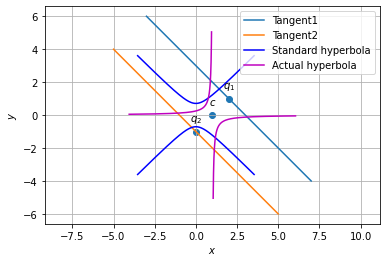
\includegraphics[width=\columnwidth]{./solutions/1/14/graph7.png}
	\caption{The standard and actual hyperbola.}
\end{figure}

  \item If A=\myvec{3 &-4\\1 &-1},\\then prove that $A^{n}$=\myvec{1+2n &-4n\\n &1-2n},where n is any positive integer\\
\\
\solution
The given curve 
\begin{align}
	y =\frac{1}{x-1}
\end{align}
can be expressed as 
\begin{align}
	xy - y - 1 = 0 \label{eq:solutions/1/14/eq:hyperbola}
\end{align}
Hence, we have
\begin{align}
	\vec{V} = \frac{1}{2}\myvec{0 & 1 \\ 1 & 0}, 
	\vec{u} = \frac{1}{2}\myvec{0 \\-1},
	f = -1
\end{align}
Since $\mydet{\vec{V}} < 0$, the equation \eqref{eq:solutions/1/14/eq:hyperbola} represents hyperbola.
To find the values of $\lambda_1$ and $\lambda_2$, consider the characteristic equation,
\begin{align}
	\mydet{\lambda\vec{I} - \vec{V}} &= 0\\
	\implies \mydet{\myvec{\lambda & 0\\0 & \lambda} - \myvec{0 & \frac{1}{2} \\ \frac{1}{2} & 0}} &= 0\\
	\implies \mydet{ \lambda & \frac{-1}{2} \\ \frac{-1}{2} & \lambda} &= 0\\
	\implies \lambda_1 &= \frac{1}{2} , \lambda_2 = \frac{-1}{2}
\end{align}
In addition, given the slope -1, the direction and normal vectors are given by 
\begin{align}
	\vec{m} = \myvec{1 \\ -1} \\
	\vec{n} = \myvec{ 1 \\ 1}
\end{align}
The parameters of hyperbola are as follows:
\begin{align}
	\vec{c} &= -\vec{V}^{-1}\vec{u} \\
	&= -\myvec{0 & 2\\ 2 & 0}\myvec{0 \\ -\frac{1}{2}} \\
	&= \myvec{1 \\ 0}\\
	axes &= \begin{cases}
	\sqrt{\frac{\vec{u}^T\vec{V}^{-1}\vec{u} - f}{\lambda_1}} = \sqrt{2}\\
 \sqrt{\frac{f-\vec{u}^T\vec{V}^{-1}\vec{u}}{\lambda_2}} = \sqrt{2}
\end{cases}
\end{align}
which represents the standard hyperbola equation,
\begin{align}
	\frac{x^2}{2} - \frac{x^2}{2} = 1
\end{align}
The points of contact are given by 
\begin{align}
  \tiny{K} &=\pm \sqrt{\frac{\vec{u}^T\vec{V}^{-1}\vec{u} - f}{\vec{n}^T\vec{V}^{-1}\vec{n}}}
  = \pm \frac{1}{2}\\
  \vec{q} &= \vec{V}^{-1}(k\vec{n}-\vec{u})\\
  \vec{q_1} &= \myvec{0 & 2\\2 & 0} \sbrak{\frac{1}{2}\myvec{1 \\ 1} - \myvec{0\\ \frac{-1}{2}}}\\
  &= \myvec{2 \\ 1}\\
  \vec{q_2} &= \myvec{0 & 2\\2 & 0} \sbrak{\frac{-1}{2}\myvec{1 \\ 1} - \myvec{0\\ \frac{-1}{2}}}\\
  &= \myvec{0 \\ -1}
\end{align} 
$\therefore$ The tangents are given by
\begin{align}
	\myvec{1 & 1} \brak{\vec{x} - \myvec{2 \\ 1}} = 0 \\
	\myvec{1 & 1} \brak{\vec{x} - \myvec{0 \\ -1}} = 0
\end{align}
The desired equations of all lines having slope -1 that are tangents to the curve $\frac{1}{x-1}, x \neq 1$ are given by
\begin{align}
	\myvec{1 & 1}\vec{x} &= 3 \\
	\myvec{1 & 1}\vec{x} &= -1 
\end{align}
The above results are verified in the following figure.
\begin{figure}[h!] \label{eq:solutions/1/14/fig:tangents}
	\centering
	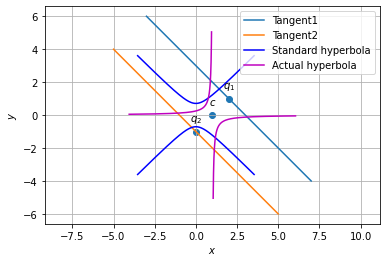
\includegraphics[width=\columnwidth]{./solutions/1/14/graph7.png}
	\caption{The standard and actual hyperbola.}
\end{figure}

  \item For what values of x: \\\myvec{1 &2 &1}\myvec{1 &2 &0\\2 &0 &1\\1 &0 &2}\myvec{0 \\2 \\x}=0?\\
\solution
The given curve 
\begin{align}
	y =\frac{1}{x-1}
\end{align}
can be expressed as 
\begin{align}
	xy - y - 1 = 0 \label{eq:solutions/1/14/eq:hyperbola}
\end{align}
Hence, we have
\begin{align}
	\vec{V} = \frac{1}{2}\myvec{0 & 1 \\ 1 & 0}, 
	\vec{u} = \frac{1}{2}\myvec{0 \\-1},
	f = -1
\end{align}
Since $\mydet{\vec{V}} < 0$, the equation \eqref{eq:solutions/1/14/eq:hyperbola} represents hyperbola.
To find the values of $\lambda_1$ and $\lambda_2$, consider the characteristic equation,
\begin{align}
	\mydet{\lambda\vec{I} - \vec{V}} &= 0\\
	\implies \mydet{\myvec{\lambda & 0\\0 & \lambda} - \myvec{0 & \frac{1}{2} \\ \frac{1}{2} & 0}} &= 0\\
	\implies \mydet{ \lambda & \frac{-1}{2} \\ \frac{-1}{2} & \lambda} &= 0\\
	\implies \lambda_1 &= \frac{1}{2} , \lambda_2 = \frac{-1}{2}
\end{align}
In addition, given the slope -1, the direction and normal vectors are given by 
\begin{align}
	\vec{m} = \myvec{1 \\ -1} \\
	\vec{n} = \myvec{ 1 \\ 1}
\end{align}
The parameters of hyperbola are as follows:
\begin{align}
	\vec{c} &= -\vec{V}^{-1}\vec{u} \\
	&= -\myvec{0 & 2\\ 2 & 0}\myvec{0 \\ -\frac{1}{2}} \\
	&= \myvec{1 \\ 0}\\
	axes &= \begin{cases}
	\sqrt{\frac{\vec{u}^T\vec{V}^{-1}\vec{u} - f}{\lambda_1}} = \sqrt{2}\\
 \sqrt{\frac{f-\vec{u}^T\vec{V}^{-1}\vec{u}}{\lambda_2}} = \sqrt{2}
\end{cases}
\end{align}
which represents the standard hyperbola equation,
\begin{align}
	\frac{x^2}{2} - \frac{x^2}{2} = 1
\end{align}
The points of contact are given by 
\begin{align}
  \tiny{K} &=\pm \sqrt{\frac{\vec{u}^T\vec{V}^{-1}\vec{u} - f}{\vec{n}^T\vec{V}^{-1}\vec{n}}}
  = \pm \frac{1}{2}\\
  \vec{q} &= \vec{V}^{-1}(k\vec{n}-\vec{u})\\
  \vec{q_1} &= \myvec{0 & 2\\2 & 0} \sbrak{\frac{1}{2}\myvec{1 \\ 1} - \myvec{0\\ \frac{-1}{2}}}\\
  &= \myvec{2 \\ 1}\\
  \vec{q_2} &= \myvec{0 & 2\\2 & 0} \sbrak{\frac{-1}{2}\myvec{1 \\ 1} - \myvec{0\\ \frac{-1}{2}}}\\
  &= \myvec{0 \\ -1}
\end{align} 
$\therefore$ The tangents are given by
\begin{align}
	\myvec{1 & 1} \brak{\vec{x} - \myvec{2 \\ 1}} = 0 \\
	\myvec{1 & 1} \brak{\vec{x} - \myvec{0 \\ -1}} = 0
\end{align}
The desired equations of all lines having slope -1 that are tangents to the curve $\frac{1}{x-1}, x \neq 1$ are given by
\begin{align}
	\myvec{1 & 1}\vec{x} &= 3 \\
	\myvec{1 & 1}\vec{x} &= -1 
\end{align}
The above results are verified in the following figure.
\begin{figure}[h!] \label{eq:solutions/1/14/fig:tangents}
	\centering
	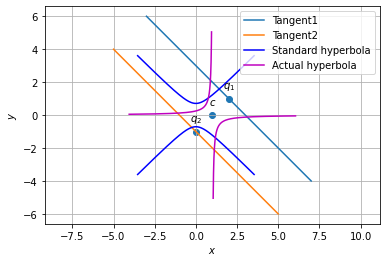
\includegraphics[width=\columnwidth]{./solutions/1/14/graph7.png}
	\caption{The standard and actual hyperbola.}
\end{figure}


  \item If A=\myvec{3 &1\\-1 &2},show that $A^{2}$-5A+7I=0\\
\solution
The given curve 
\begin{align}
	y =\frac{1}{x-1}
\end{align}
can be expressed as 
\begin{align}
	xy - y - 1 = 0 \label{eq:solutions/1/14/eq:hyperbola}
\end{align}
Hence, we have
\begin{align}
	\vec{V} = \frac{1}{2}\myvec{0 & 1 \\ 1 & 0}, 
	\vec{u} = \frac{1}{2}\myvec{0 \\-1},
	f = -1
\end{align}
Since $\mydet{\vec{V}} < 0$, the equation \eqref{eq:solutions/1/14/eq:hyperbola} represents hyperbola.
To find the values of $\lambda_1$ and $\lambda_2$, consider the characteristic equation,
\begin{align}
	\mydet{\lambda\vec{I} - \vec{V}} &= 0\\
	\implies \mydet{\myvec{\lambda & 0\\0 & \lambda} - \myvec{0 & \frac{1}{2} \\ \frac{1}{2} & 0}} &= 0\\
	\implies \mydet{ \lambda & \frac{-1}{2} \\ \frac{-1}{2} & \lambda} &= 0\\
	\implies \lambda_1 &= \frac{1}{2} , \lambda_2 = \frac{-1}{2}
\end{align}
In addition, given the slope -1, the direction and normal vectors are given by 
\begin{align}
	\vec{m} = \myvec{1 \\ -1} \\
	\vec{n} = \myvec{ 1 \\ 1}
\end{align}
The parameters of hyperbola are as follows:
\begin{align}
	\vec{c} &= -\vec{V}^{-1}\vec{u} \\
	&= -\myvec{0 & 2\\ 2 & 0}\myvec{0 \\ -\frac{1}{2}} \\
	&= \myvec{1 \\ 0}\\
	axes &= \begin{cases}
	\sqrt{\frac{\vec{u}^T\vec{V}^{-1}\vec{u} - f}{\lambda_1}} = \sqrt{2}\\
 \sqrt{\frac{f-\vec{u}^T\vec{V}^{-1}\vec{u}}{\lambda_2}} = \sqrt{2}
\end{cases}
\end{align}
which represents the standard hyperbola equation,
\begin{align}
	\frac{x^2}{2} - \frac{x^2}{2} = 1
\end{align}
The points of contact are given by 
\begin{align}
  \tiny{K} &=\pm \sqrt{\frac{\vec{u}^T\vec{V}^{-1}\vec{u} - f}{\vec{n}^T\vec{V}^{-1}\vec{n}}}
  = \pm \frac{1}{2}\\
  \vec{q} &= \vec{V}^{-1}(k\vec{n}-\vec{u})\\
  \vec{q_1} &= \myvec{0 & 2\\2 & 0} \sbrak{\frac{1}{2}\myvec{1 \\ 1} - \myvec{0\\ \frac{-1}{2}}}\\
  &= \myvec{2 \\ 1}\\
  \vec{q_2} &= \myvec{0 & 2\\2 & 0} \sbrak{\frac{-1}{2}\myvec{1 \\ 1} - \myvec{0\\ \frac{-1}{2}}}\\
  &= \myvec{0 \\ -1}
\end{align} 
$\therefore$ The tangents are given by
\begin{align}
	\myvec{1 & 1} \brak{\vec{x} - \myvec{2 \\ 1}} = 0 \\
	\myvec{1 & 1} \brak{\vec{x} - \myvec{0 \\ -1}} = 0
\end{align}
The desired equations of all lines having slope -1 that are tangents to the curve $\frac{1}{x-1}, x \neq 1$ are given by
\begin{align}
	\myvec{1 & 1}\vec{x} &= 3 \\
	\myvec{1 & 1}\vec{x} &= -1 
\end{align}
The above results are verified in the following figure.
\begin{figure}[h!] \label{eq:solutions/1/14/fig:tangents}
	\centering
	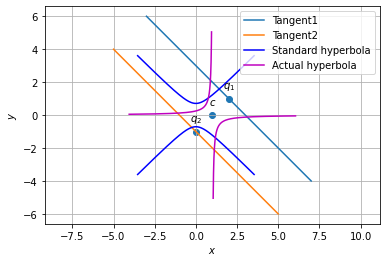
\includegraphics[width=\columnwidth]{./solutions/1/14/graph7.png}
	\caption{The standard and actual hyperbola.}
\end{figure}


%\end{enumerate}
%\end{document}
    

%\renewcommand{\theequation}{\theenumi}
%\begin{enumerate}[label=\arabic*.,ref=\thesubsection.\theenumi]
%\numberwithin{equation}{enumi}

\item Find 
$\begin{vmatrix}
2&4\\-5&-1
\end{vmatrix}$
\\
\solution 
The given curve 
\begin{align}
	y =\frac{1}{x-1}
\end{align}
can be expressed as 
\begin{align}
	xy - y - 1 = 0 \label{eq:solutions/1/14/eq:hyperbola}
\end{align}
Hence, we have
\begin{align}
	\vec{V} = \frac{1}{2}\myvec{0 & 1 \\ 1 & 0}, 
	\vec{u} = \frac{1}{2}\myvec{0 \\-1},
	f = -1
\end{align}
Since $\mydet{\vec{V}} < 0$, the equation \eqref{eq:solutions/1/14/eq:hyperbola} represents hyperbola.
To find the values of $\lambda_1$ and $\lambda_2$, consider the characteristic equation,
\begin{align}
	\mydet{\lambda\vec{I} - \vec{V}} &= 0\\
	\implies \mydet{\myvec{\lambda & 0\\0 & \lambda} - \myvec{0 & \frac{1}{2} \\ \frac{1}{2} & 0}} &= 0\\
	\implies \mydet{ \lambda & \frac{-1}{2} \\ \frac{-1}{2} & \lambda} &= 0\\
	\implies \lambda_1 &= \frac{1}{2} , \lambda_2 = \frac{-1}{2}
\end{align}
In addition, given the slope -1, the direction and normal vectors are given by 
\begin{align}
	\vec{m} = \myvec{1 \\ -1} \\
	\vec{n} = \myvec{ 1 \\ 1}
\end{align}
The parameters of hyperbola are as follows:
\begin{align}
	\vec{c} &= -\vec{V}^{-1}\vec{u} \\
	&= -\myvec{0 & 2\\ 2 & 0}\myvec{0 \\ -\frac{1}{2}} \\
	&= \myvec{1 \\ 0}\\
	axes &= \begin{cases}
	\sqrt{\frac{\vec{u}^T\vec{V}^{-1}\vec{u} - f}{\lambda_1}} = \sqrt{2}\\
 \sqrt{\frac{f-\vec{u}^T\vec{V}^{-1}\vec{u}}{\lambda_2}} = \sqrt{2}
\end{cases}
\end{align}
which represents the standard hyperbola equation,
\begin{align}
	\frac{x^2}{2} - \frac{x^2}{2} = 1
\end{align}
The points of contact are given by 
\begin{align}
  \tiny{K} &=\pm \sqrt{\frac{\vec{u}^T\vec{V}^{-1}\vec{u} - f}{\vec{n}^T\vec{V}^{-1}\vec{n}}}
  = \pm \frac{1}{2}\\
  \vec{q} &= \vec{V}^{-1}(k\vec{n}-\vec{u})\\
  \vec{q_1} &= \myvec{0 & 2\\2 & 0} \sbrak{\frac{1}{2}\myvec{1 \\ 1} - \myvec{0\\ \frac{-1}{2}}}\\
  &= \myvec{2 \\ 1}\\
  \vec{q_2} &= \myvec{0 & 2\\2 & 0} \sbrak{\frac{-1}{2}\myvec{1 \\ 1} - \myvec{0\\ \frac{-1}{2}}}\\
  &= \myvec{0 \\ -1}
\end{align} 
$\therefore$ The tangents are given by
\begin{align}
	\myvec{1 & 1} \brak{\vec{x} - \myvec{2 \\ 1}} = 0 \\
	\myvec{1 & 1} \brak{\vec{x} - \myvec{0 \\ -1}} = 0
\end{align}
The desired equations of all lines having slope -1 that are tangents to the curve $\frac{1}{x-1}, x \neq 1$ are given by
\begin{align}
	\myvec{1 & 1}\vec{x} &= 3 \\
	\myvec{1 & 1}\vec{x} &= -1 
\end{align}
The above results are verified in the following figure.
\begin{figure}[h!] \label{eq:solutions/1/14/fig:tangents}
	\centering
	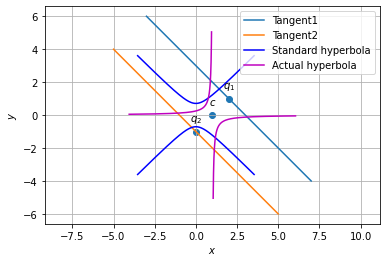
\includegraphics[width=\columnwidth]{./solutions/1/14/graph7.png}
	\caption{The standard and actual hyperbola.}
\end{figure}


\item (i) $\begin{vmatrix}\cos\theta& -\sin\theta\\ \sin\theta& \cos\theta \end{vmatrix}$ 
(ii) $\begin{vmatrix}
x^2-x+1& x-1\\ x+1&  x+1
\end{vmatrix}$
\\
\solution 
The given curve 
\begin{align}
	y =\frac{1}{x-1}
\end{align}
can be expressed as 
\begin{align}
	xy - y - 1 = 0 \label{eq:solutions/1/14/eq:hyperbola}
\end{align}
Hence, we have
\begin{align}
	\vec{V} = \frac{1}{2}\myvec{0 & 1 \\ 1 & 0}, 
	\vec{u} = \frac{1}{2}\myvec{0 \\-1},
	f = -1
\end{align}
Since $\mydet{\vec{V}} < 0$, the equation \eqref{eq:solutions/1/14/eq:hyperbola} represents hyperbola.
To find the values of $\lambda_1$ and $\lambda_2$, consider the characteristic equation,
\begin{align}
	\mydet{\lambda\vec{I} - \vec{V}} &= 0\\
	\implies \mydet{\myvec{\lambda & 0\\0 & \lambda} - \myvec{0 & \frac{1}{2} \\ \frac{1}{2} & 0}} &= 0\\
	\implies \mydet{ \lambda & \frac{-1}{2} \\ \frac{-1}{2} & \lambda} &= 0\\
	\implies \lambda_1 &= \frac{1}{2} , \lambda_2 = \frac{-1}{2}
\end{align}
In addition, given the slope -1, the direction and normal vectors are given by 
\begin{align}
	\vec{m} = \myvec{1 \\ -1} \\
	\vec{n} = \myvec{ 1 \\ 1}
\end{align}
The parameters of hyperbola are as follows:
\begin{align}
	\vec{c} &= -\vec{V}^{-1}\vec{u} \\
	&= -\myvec{0 & 2\\ 2 & 0}\myvec{0 \\ -\frac{1}{2}} \\
	&= \myvec{1 \\ 0}\\
	axes &= \begin{cases}
	\sqrt{\frac{\vec{u}^T\vec{V}^{-1}\vec{u} - f}{\lambda_1}} = \sqrt{2}\\
 \sqrt{\frac{f-\vec{u}^T\vec{V}^{-1}\vec{u}}{\lambda_2}} = \sqrt{2}
\end{cases}
\end{align}
which represents the standard hyperbola equation,
\begin{align}
	\frac{x^2}{2} - \frac{x^2}{2} = 1
\end{align}
The points of contact are given by 
\begin{align}
  \tiny{K} &=\pm \sqrt{\frac{\vec{u}^T\vec{V}^{-1}\vec{u} - f}{\vec{n}^T\vec{V}^{-1}\vec{n}}}
  = \pm \frac{1}{2}\\
  \vec{q} &= \vec{V}^{-1}(k\vec{n}-\vec{u})\\
  \vec{q_1} &= \myvec{0 & 2\\2 & 0} \sbrak{\frac{1}{2}\myvec{1 \\ 1} - \myvec{0\\ \frac{-1}{2}}}\\
  &= \myvec{2 \\ 1}\\
  \vec{q_2} &= \myvec{0 & 2\\2 & 0} \sbrak{\frac{-1}{2}\myvec{1 \\ 1} - \myvec{0\\ \frac{-1}{2}}}\\
  &= \myvec{0 \\ -1}
\end{align} 
$\therefore$ The tangents are given by
\begin{align}
	\myvec{1 & 1} \brak{\vec{x} - \myvec{2 \\ 1}} = 0 \\
	\myvec{1 & 1} \brak{\vec{x} - \myvec{0 \\ -1}} = 0
\end{align}
The desired equations of all lines having slope -1 that are tangents to the curve $\frac{1}{x-1}, x \neq 1$ are given by
\begin{align}
	\myvec{1 & 1}\vec{x} &= 3 \\
	\myvec{1 & 1}\vec{x} &= -1 
\end{align}
The above results are verified in the following figure.
\begin{figure}[h!] \label{eq:solutions/1/14/fig:tangents}
	\centering
	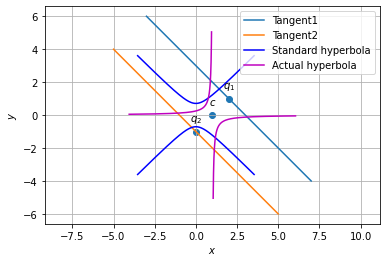
\includegraphics[width=\columnwidth]{./solutions/1/14/graph7.png}
	\caption{The standard and actual hyperbola.}
\end{figure}

\item If$ \vec{A} = \begin{vmatrix}1&2\\4&2\end{vmatrix}$,then show that  
$\abs{2\vec{A}}=4\abs{\vec{A}}$
\\
\solution 
The given curve 
\begin{align}
	y =\frac{1}{x-1}
\end{align}
can be expressed as 
\begin{align}
	xy - y - 1 = 0 \label{eq:solutions/1/14/eq:hyperbola}
\end{align}
Hence, we have
\begin{align}
	\vec{V} = \frac{1}{2}\myvec{0 & 1 \\ 1 & 0}, 
	\vec{u} = \frac{1}{2}\myvec{0 \\-1},
	f = -1
\end{align}
Since $\mydet{\vec{V}} < 0$, the equation \eqref{eq:solutions/1/14/eq:hyperbola} represents hyperbola.
To find the values of $\lambda_1$ and $\lambda_2$, consider the characteristic equation,
\begin{align}
	\mydet{\lambda\vec{I} - \vec{V}} &= 0\\
	\implies \mydet{\myvec{\lambda & 0\\0 & \lambda} - \myvec{0 & \frac{1}{2} \\ \frac{1}{2} & 0}} &= 0\\
	\implies \mydet{ \lambda & \frac{-1}{2} \\ \frac{-1}{2} & \lambda} &= 0\\
	\implies \lambda_1 &= \frac{1}{2} , \lambda_2 = \frac{-1}{2}
\end{align}
In addition, given the slope -1, the direction and normal vectors are given by 
\begin{align}
	\vec{m} = \myvec{1 \\ -1} \\
	\vec{n} = \myvec{ 1 \\ 1}
\end{align}
The parameters of hyperbola are as follows:
\begin{align}
	\vec{c} &= -\vec{V}^{-1}\vec{u} \\
	&= -\myvec{0 & 2\\ 2 & 0}\myvec{0 \\ -\frac{1}{2}} \\
	&= \myvec{1 \\ 0}\\
	axes &= \begin{cases}
	\sqrt{\frac{\vec{u}^T\vec{V}^{-1}\vec{u} - f}{\lambda_1}} = \sqrt{2}\\
 \sqrt{\frac{f-\vec{u}^T\vec{V}^{-1}\vec{u}}{\lambda_2}} = \sqrt{2}
\end{cases}
\end{align}
which represents the standard hyperbola equation,
\begin{align}
	\frac{x^2}{2} - \frac{x^2}{2} = 1
\end{align}
The points of contact are given by 
\begin{align}
  \tiny{K} &=\pm \sqrt{\frac{\vec{u}^T\vec{V}^{-1}\vec{u} - f}{\vec{n}^T\vec{V}^{-1}\vec{n}}}
  = \pm \frac{1}{2}\\
  \vec{q} &= \vec{V}^{-1}(k\vec{n}-\vec{u})\\
  \vec{q_1} &= \myvec{0 & 2\\2 & 0} \sbrak{\frac{1}{2}\myvec{1 \\ 1} - \myvec{0\\ \frac{-1}{2}}}\\
  &= \myvec{2 \\ 1}\\
  \vec{q_2} &= \myvec{0 & 2\\2 & 0} \sbrak{\frac{-1}{2}\myvec{1 \\ 1} - \myvec{0\\ \frac{-1}{2}}}\\
  &= \myvec{0 \\ -1}
\end{align} 
$\therefore$ The tangents are given by
\begin{align}
	\myvec{1 & 1} \brak{\vec{x} - \myvec{2 \\ 1}} = 0 \\
	\myvec{1 & 1} \brak{\vec{x} - \myvec{0 \\ -1}} = 0
\end{align}
The desired equations of all lines having slope -1 that are tangents to the curve $\frac{1}{x-1}, x \neq 1$ are given by
\begin{align}
	\myvec{1 & 1}\vec{x} &= 3 \\
	\myvec{1 & 1}\vec{x} &= -1 
\end{align}
The above results are verified in the following figure.
\begin{figure}[h!] \label{eq:solutions/1/14/fig:tangents}
	\centering
	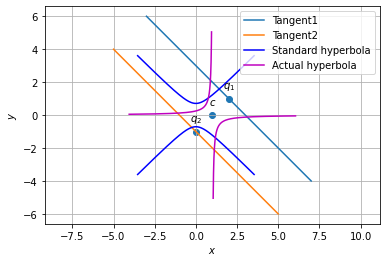
\includegraphics[width=\columnwidth]{./solutions/1/14/graph7.png}
	\caption{The standard and actual hyperbola.}
\end{figure}

\item If $\vec{A}=\begin{vmatrix}1&0&1\\0&1&2\\0&0&4\end{vmatrix}$, then show that $\abs{3\vec{A}}=27\abs{\vec{A}}$
\\
\solution 
The given curve 
\begin{align}
	y =\frac{1}{x-1}
\end{align}
can be expressed as 
\begin{align}
	xy - y - 1 = 0 \label{eq:solutions/1/14/eq:hyperbola}
\end{align}
Hence, we have
\begin{align}
	\vec{V} = \frac{1}{2}\myvec{0 & 1 \\ 1 & 0}, 
	\vec{u} = \frac{1}{2}\myvec{0 \\-1},
	f = -1
\end{align}
Since $\mydet{\vec{V}} < 0$, the equation \eqref{eq:solutions/1/14/eq:hyperbola} represents hyperbola.
To find the values of $\lambda_1$ and $\lambda_2$, consider the characteristic equation,
\begin{align}
	\mydet{\lambda\vec{I} - \vec{V}} &= 0\\
	\implies \mydet{\myvec{\lambda & 0\\0 & \lambda} - \myvec{0 & \frac{1}{2} \\ \frac{1}{2} & 0}} &= 0\\
	\implies \mydet{ \lambda & \frac{-1}{2} \\ \frac{-1}{2} & \lambda} &= 0\\
	\implies \lambda_1 &= \frac{1}{2} , \lambda_2 = \frac{-1}{2}
\end{align}
In addition, given the slope -1, the direction and normal vectors are given by 
\begin{align}
	\vec{m} = \myvec{1 \\ -1} \\
	\vec{n} = \myvec{ 1 \\ 1}
\end{align}
The parameters of hyperbola are as follows:
\begin{align}
	\vec{c} &= -\vec{V}^{-1}\vec{u} \\
	&= -\myvec{0 & 2\\ 2 & 0}\myvec{0 \\ -\frac{1}{2}} \\
	&= \myvec{1 \\ 0}\\
	axes &= \begin{cases}
	\sqrt{\frac{\vec{u}^T\vec{V}^{-1}\vec{u} - f}{\lambda_1}} = \sqrt{2}\\
 \sqrt{\frac{f-\vec{u}^T\vec{V}^{-1}\vec{u}}{\lambda_2}} = \sqrt{2}
\end{cases}
\end{align}
which represents the standard hyperbola equation,
\begin{align}
	\frac{x^2}{2} - \frac{x^2}{2} = 1
\end{align}
The points of contact are given by 
\begin{align}
  \tiny{K} &=\pm \sqrt{\frac{\vec{u}^T\vec{V}^{-1}\vec{u} - f}{\vec{n}^T\vec{V}^{-1}\vec{n}}}
  = \pm \frac{1}{2}\\
  \vec{q} &= \vec{V}^{-1}(k\vec{n}-\vec{u})\\
  \vec{q_1} &= \myvec{0 & 2\\2 & 0} \sbrak{\frac{1}{2}\myvec{1 \\ 1} - \myvec{0\\ \frac{-1}{2}}}\\
  &= \myvec{2 \\ 1}\\
  \vec{q_2} &= \myvec{0 & 2\\2 & 0} \sbrak{\frac{-1}{2}\myvec{1 \\ 1} - \myvec{0\\ \frac{-1}{2}}}\\
  &= \myvec{0 \\ -1}
\end{align} 
$\therefore$ The tangents are given by
\begin{align}
	\myvec{1 & 1} \brak{\vec{x} - \myvec{2 \\ 1}} = 0 \\
	\myvec{1 & 1} \brak{\vec{x} - \myvec{0 \\ -1}} = 0
\end{align}
The desired equations of all lines having slope -1 that are tangents to the curve $\frac{1}{x-1}, x \neq 1$ are given by
\begin{align}
	\myvec{1 & 1}\vec{x} &= 3 \\
	\myvec{1 & 1}\vec{x} &= -1 
\end{align}
The above results are verified in the following figure.
\begin{figure}[h!] \label{eq:solutions/1/14/fig:tangents}
	\centering
	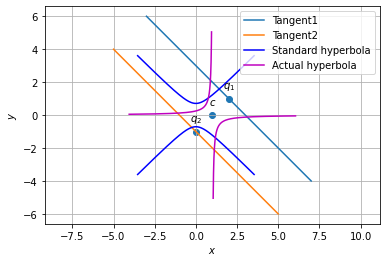
\includegraphics[width=\columnwidth]{./solutions/1/14/graph7.png}
	\caption{The standard and actual hyperbola.}
\end{figure}

\item Evaluate the determinants
\begin{enumerate}
\item $\begin{vmatrix}
3&-1&-2\\0&0&-1\\3&-5&0
\end{vmatrix}$
\item $\begin{vmatrix}
3&-4&5\\1&1&-2\\2&3&1
\end{vmatrix}$
\\
\solution 

The following python code computes the required determinant value.
	\begin{lstlisting}
	./solutions/5/codes/lines/q14.py
	\end{lstlisting}
	
	\begin{enumerate}
		\item $\mydet{3&-1&-2\\0&0&-1\\3&-5&0} = -12$
		\item $\mydet{3&-4&5\\1&1&-2\\2&3&1} = -46$
		\item $\mydet{0&1&2\\-1&0&-3\\-2&3&0}=0$
		\item $\mydet{2&-1&-2\\0&2&-1\\3&-5&0} = 5$

	\end{enumerate}

\item $\begin{vmatrix}
0&1&2 \\ -1&0&-3\\-2&3&0
\end{vmatrix}$
\item $\begin{vmatrix}
2&-1&-2\\0&2&-1\\3&-5&0
\end{vmatrix}$
\end{enumerate}  
\item If A=$\begin{vmatrix}1&1&-2\\2&1&-3\\5&4&-9\end{vmatrix}$, 
find $\abs{A}$
\\
\solution 
The given curve 
\begin{align}
	y =\frac{1}{x-1}
\end{align}
can be expressed as 
\begin{align}
	xy - y - 1 = 0 \label{eq:solutions/1/14/eq:hyperbola}
\end{align}
Hence, we have
\begin{align}
	\vec{V} = \frac{1}{2}\myvec{0 & 1 \\ 1 & 0}, 
	\vec{u} = \frac{1}{2}\myvec{0 \\-1},
	f = -1
\end{align}
Since $\mydet{\vec{V}} < 0$, the equation \eqref{eq:solutions/1/14/eq:hyperbola} represents hyperbola.
To find the values of $\lambda_1$ and $\lambda_2$, consider the characteristic equation,
\begin{align}
	\mydet{\lambda\vec{I} - \vec{V}} &= 0\\
	\implies \mydet{\myvec{\lambda & 0\\0 & \lambda} - \myvec{0 & \frac{1}{2} \\ \frac{1}{2} & 0}} &= 0\\
	\implies \mydet{ \lambda & \frac{-1}{2} \\ \frac{-1}{2} & \lambda} &= 0\\
	\implies \lambda_1 &= \frac{1}{2} , \lambda_2 = \frac{-1}{2}
\end{align}
In addition, given the slope -1, the direction and normal vectors are given by 
\begin{align}
	\vec{m} = \myvec{1 \\ -1} \\
	\vec{n} = \myvec{ 1 \\ 1}
\end{align}
The parameters of hyperbola are as follows:
\begin{align}
	\vec{c} &= -\vec{V}^{-1}\vec{u} \\
	&= -\myvec{0 & 2\\ 2 & 0}\myvec{0 \\ -\frac{1}{2}} \\
	&= \myvec{1 \\ 0}\\
	axes &= \begin{cases}
	\sqrt{\frac{\vec{u}^T\vec{V}^{-1}\vec{u} - f}{\lambda_1}} = \sqrt{2}\\
 \sqrt{\frac{f-\vec{u}^T\vec{V}^{-1}\vec{u}}{\lambda_2}} = \sqrt{2}
\end{cases}
\end{align}
which represents the standard hyperbola equation,
\begin{align}
	\frac{x^2}{2} - \frac{x^2}{2} = 1
\end{align}
The points of contact are given by 
\begin{align}
  \tiny{K} &=\pm \sqrt{\frac{\vec{u}^T\vec{V}^{-1}\vec{u} - f}{\vec{n}^T\vec{V}^{-1}\vec{n}}}
  = \pm \frac{1}{2}\\
  \vec{q} &= \vec{V}^{-1}(k\vec{n}-\vec{u})\\
  \vec{q_1} &= \myvec{0 & 2\\2 & 0} \sbrak{\frac{1}{2}\myvec{1 \\ 1} - \myvec{0\\ \frac{-1}{2}}}\\
  &= \myvec{2 \\ 1}\\
  \vec{q_2} &= \myvec{0 & 2\\2 & 0} \sbrak{\frac{-1}{2}\myvec{1 \\ 1} - \myvec{0\\ \frac{-1}{2}}}\\
  &= \myvec{0 \\ -1}
\end{align} 
$\therefore$ The tangents are given by
\begin{align}
	\myvec{1 & 1} \brak{\vec{x} - \myvec{2 \\ 1}} = 0 \\
	\myvec{1 & 1} \brak{\vec{x} - \myvec{0 \\ -1}} = 0
\end{align}
The desired equations of all lines having slope -1 that are tangents to the curve $\frac{1}{x-1}, x \neq 1$ are given by
\begin{align}
	\myvec{1 & 1}\vec{x} &= 3 \\
	\myvec{1 & 1}\vec{x} &= -1 
\end{align}
The above results are verified in the following figure.
\begin{figure}[h!] \label{eq:solutions/1/14/fig:tangents}
	\centering
	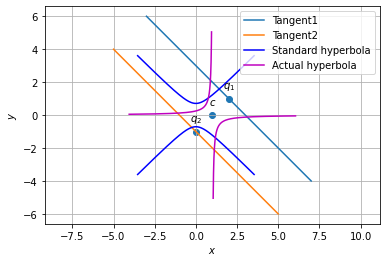
\includegraphics[width=\columnwidth]{./solutions/1/14/graph7.png}
	\caption{The standard and actual hyperbola.}
\end{figure}

\item Find the values of x,If\\
(i)$\begin{vmatrix}
2&4\\5&1
\end{vmatrix}$ =$\begin{vmatrix}
2x&4 \\ 6&x
\end{vmatrix}$
(ii)$\begin{vmatrix}
2&3 \\ 4&5
\end{vmatrix}$ =$\begin{vmatrix}
x&3 \\ 2x&5
\end{vmatrix}$
\\
\solution 
The given curve 
\begin{align}
	y =\frac{1}{x-1}
\end{align}
can be expressed as 
\begin{align}
	xy - y - 1 = 0 \label{eq:solutions/1/14/eq:hyperbola}
\end{align}
Hence, we have
\begin{align}
	\vec{V} = \frac{1}{2}\myvec{0 & 1 \\ 1 & 0}, 
	\vec{u} = \frac{1}{2}\myvec{0 \\-1},
	f = -1
\end{align}
Since $\mydet{\vec{V}} < 0$, the equation \eqref{eq:solutions/1/14/eq:hyperbola} represents hyperbola.
To find the values of $\lambda_1$ and $\lambda_2$, consider the characteristic equation,
\begin{align}
	\mydet{\lambda\vec{I} - \vec{V}} &= 0\\
	\implies \mydet{\myvec{\lambda & 0\\0 & \lambda} - \myvec{0 & \frac{1}{2} \\ \frac{1}{2} & 0}} &= 0\\
	\implies \mydet{ \lambda & \frac{-1}{2} \\ \frac{-1}{2} & \lambda} &= 0\\
	\implies \lambda_1 &= \frac{1}{2} , \lambda_2 = \frac{-1}{2}
\end{align}
In addition, given the slope -1, the direction and normal vectors are given by 
\begin{align}
	\vec{m} = \myvec{1 \\ -1} \\
	\vec{n} = \myvec{ 1 \\ 1}
\end{align}
The parameters of hyperbola are as follows:
\begin{align}
	\vec{c} &= -\vec{V}^{-1}\vec{u} \\
	&= -\myvec{0 & 2\\ 2 & 0}\myvec{0 \\ -\frac{1}{2}} \\
	&= \myvec{1 \\ 0}\\
	axes &= \begin{cases}
	\sqrt{\frac{\vec{u}^T\vec{V}^{-1}\vec{u} - f}{\lambda_1}} = \sqrt{2}\\
 \sqrt{\frac{f-\vec{u}^T\vec{V}^{-1}\vec{u}}{\lambda_2}} = \sqrt{2}
\end{cases}
\end{align}
which represents the standard hyperbola equation,
\begin{align}
	\frac{x^2}{2} - \frac{x^2}{2} = 1
\end{align}
The points of contact are given by 
\begin{align}
  \tiny{K} &=\pm \sqrt{\frac{\vec{u}^T\vec{V}^{-1}\vec{u} - f}{\vec{n}^T\vec{V}^{-1}\vec{n}}}
  = \pm \frac{1}{2}\\
  \vec{q} &= \vec{V}^{-1}(k\vec{n}-\vec{u})\\
  \vec{q_1} &= \myvec{0 & 2\\2 & 0} \sbrak{\frac{1}{2}\myvec{1 \\ 1} - \myvec{0\\ \frac{-1}{2}}}\\
  &= \myvec{2 \\ 1}\\
  \vec{q_2} &= \myvec{0 & 2\\2 & 0} \sbrak{\frac{-1}{2}\myvec{1 \\ 1} - \myvec{0\\ \frac{-1}{2}}}\\
  &= \myvec{0 \\ -1}
\end{align} 
$\therefore$ The tangents are given by
\begin{align}
	\myvec{1 & 1} \brak{\vec{x} - \myvec{2 \\ 1}} = 0 \\
	\myvec{1 & 1} \brak{\vec{x} - \myvec{0 \\ -1}} = 0
\end{align}
The desired equations of all lines having slope -1 that are tangents to the curve $\frac{1}{x-1}, x \neq 1$ are given by
\begin{align}
	\myvec{1 & 1}\vec{x} &= 3 \\
	\myvec{1 & 1}\vec{x} &= -1 
\end{align}
The above results are verified in the following figure.
\begin{figure}[h!] \label{eq:solutions/1/14/fig:tangents}
	\centering
	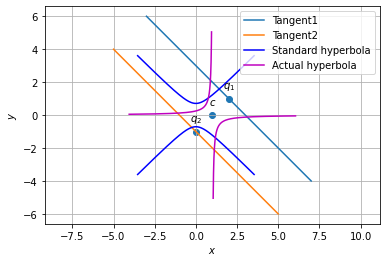
\includegraphics[width=\columnwidth]{./solutions/1/14/graph7.png}
	\caption{The standard and actual hyperbola.}
\end{figure}

\item If  $\begin{vmatrix}
x&2 \\ 18&x
\end{vmatrix}$ =$\begin{vmatrix}
6&2 \\ 18&6
\end{vmatrix}$, then x is equal to 
\begin{enumerate}
\item 6
\item $\pm 6$
\item $-6$
\item 0
\end{enumerate}
\item $\begin{vmatrix}
x&a&x+a\\y&b&y+b\\z&c&z+c\end{vmatrix}=0$
\\
\solution 
The given curve 
\begin{align}
	y =\frac{1}{x-1}
\end{align}
can be expressed as 
\begin{align}
	xy - y - 1 = 0 \label{eq:solutions/1/14/eq:hyperbola}
\end{align}
Hence, we have
\begin{align}
	\vec{V} = \frac{1}{2}\myvec{0 & 1 \\ 1 & 0}, 
	\vec{u} = \frac{1}{2}\myvec{0 \\-1},
	f = -1
\end{align}
Since $\mydet{\vec{V}} < 0$, the equation \eqref{eq:solutions/1/14/eq:hyperbola} represents hyperbola.
To find the values of $\lambda_1$ and $\lambda_2$, consider the characteristic equation,
\begin{align}
	\mydet{\lambda\vec{I} - \vec{V}} &= 0\\
	\implies \mydet{\myvec{\lambda & 0\\0 & \lambda} - \myvec{0 & \frac{1}{2} \\ \frac{1}{2} & 0}} &= 0\\
	\implies \mydet{ \lambda & \frac{-1}{2} \\ \frac{-1}{2} & \lambda} &= 0\\
	\implies \lambda_1 &= \frac{1}{2} , \lambda_2 = \frac{-1}{2}
\end{align}
In addition, given the slope -1, the direction and normal vectors are given by 
\begin{align}
	\vec{m} = \myvec{1 \\ -1} \\
	\vec{n} = \myvec{ 1 \\ 1}
\end{align}
The parameters of hyperbola are as follows:
\begin{align}
	\vec{c} &= -\vec{V}^{-1}\vec{u} \\
	&= -\myvec{0 & 2\\ 2 & 0}\myvec{0 \\ -\frac{1}{2}} \\
	&= \myvec{1 \\ 0}\\
	axes &= \begin{cases}
	\sqrt{\frac{\vec{u}^T\vec{V}^{-1}\vec{u} - f}{\lambda_1}} = \sqrt{2}\\
 \sqrt{\frac{f-\vec{u}^T\vec{V}^{-1}\vec{u}}{\lambda_2}} = \sqrt{2}
\end{cases}
\end{align}
which represents the standard hyperbola equation,
\begin{align}
	\frac{x^2}{2} - \frac{x^2}{2} = 1
\end{align}
The points of contact are given by 
\begin{align}
  \tiny{K} &=\pm \sqrt{\frac{\vec{u}^T\vec{V}^{-1}\vec{u} - f}{\vec{n}^T\vec{V}^{-1}\vec{n}}}
  = \pm \frac{1}{2}\\
  \vec{q} &= \vec{V}^{-1}(k\vec{n}-\vec{u})\\
  \vec{q_1} &= \myvec{0 & 2\\2 & 0} \sbrak{\frac{1}{2}\myvec{1 \\ 1} - \myvec{0\\ \frac{-1}{2}}}\\
  &= \myvec{2 \\ 1}\\
  \vec{q_2} &= \myvec{0 & 2\\2 & 0} \sbrak{\frac{-1}{2}\myvec{1 \\ 1} - \myvec{0\\ \frac{-1}{2}}}\\
  &= \myvec{0 \\ -1}
\end{align} 
$\therefore$ The tangents are given by
\begin{align}
	\myvec{1 & 1} \brak{\vec{x} - \myvec{2 \\ 1}} = 0 \\
	\myvec{1 & 1} \brak{\vec{x} - \myvec{0 \\ -1}} = 0
\end{align}
The desired equations of all lines having slope -1 that are tangents to the curve $\frac{1}{x-1}, x \neq 1$ are given by
\begin{align}
	\myvec{1 & 1}\vec{x} &= 3 \\
	\myvec{1 & 1}\vec{x} &= -1 
\end{align}
The above results are verified in the following figure.
\begin{figure}[h!] \label{eq:solutions/1/14/fig:tangents}
	\centering
	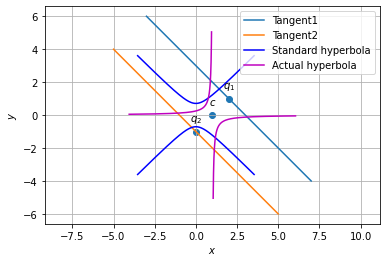
\includegraphics[width=\columnwidth]{./solutions/1/14/graph7.png}
	\caption{The standard and actual hyperbola.}
\end{figure}

\item $\begin{vmatrix}
a-b&b-c&c-a\\b-c&c-a&a-b\\c-a&a-b&b-c\end{vmatrix}=0$
\\
\solution 
The given curve 
\begin{align}
	y =\frac{1}{x-1}
\end{align}
can be expressed as 
\begin{align}
	xy - y - 1 = 0 \label{eq:solutions/1/14/eq:hyperbola}
\end{align}
Hence, we have
\begin{align}
	\vec{V} = \frac{1}{2}\myvec{0 & 1 \\ 1 & 0}, 
	\vec{u} = \frac{1}{2}\myvec{0 \\-1},
	f = -1
\end{align}
Since $\mydet{\vec{V}} < 0$, the equation \eqref{eq:solutions/1/14/eq:hyperbola} represents hyperbola.
To find the values of $\lambda_1$ and $\lambda_2$, consider the characteristic equation,
\begin{align}
	\mydet{\lambda\vec{I} - \vec{V}} &= 0\\
	\implies \mydet{\myvec{\lambda & 0\\0 & \lambda} - \myvec{0 & \frac{1}{2} \\ \frac{1}{2} & 0}} &= 0\\
	\implies \mydet{ \lambda & \frac{-1}{2} \\ \frac{-1}{2} & \lambda} &= 0\\
	\implies \lambda_1 &= \frac{1}{2} , \lambda_2 = \frac{-1}{2}
\end{align}
In addition, given the slope -1, the direction and normal vectors are given by 
\begin{align}
	\vec{m} = \myvec{1 \\ -1} \\
	\vec{n} = \myvec{ 1 \\ 1}
\end{align}
The parameters of hyperbola are as follows:
\begin{align}
	\vec{c} &= -\vec{V}^{-1}\vec{u} \\
	&= -\myvec{0 & 2\\ 2 & 0}\myvec{0 \\ -\frac{1}{2}} \\
	&= \myvec{1 \\ 0}\\
	axes &= \begin{cases}
	\sqrt{\frac{\vec{u}^T\vec{V}^{-1}\vec{u} - f}{\lambda_1}} = \sqrt{2}\\
 \sqrt{\frac{f-\vec{u}^T\vec{V}^{-1}\vec{u}}{\lambda_2}} = \sqrt{2}
\end{cases}
\end{align}
which represents the standard hyperbola equation,
\begin{align}
	\frac{x^2}{2} - \frac{x^2}{2} = 1
\end{align}
The points of contact are given by 
\begin{align}
  \tiny{K} &=\pm \sqrt{\frac{\vec{u}^T\vec{V}^{-1}\vec{u} - f}{\vec{n}^T\vec{V}^{-1}\vec{n}}}
  = \pm \frac{1}{2}\\
  \vec{q} &= \vec{V}^{-1}(k\vec{n}-\vec{u})\\
  \vec{q_1} &= \myvec{0 & 2\\2 & 0} \sbrak{\frac{1}{2}\myvec{1 \\ 1} - \myvec{0\\ \frac{-1}{2}}}\\
  &= \myvec{2 \\ 1}\\
  \vec{q_2} &= \myvec{0 & 2\\2 & 0} \sbrak{\frac{-1}{2}\myvec{1 \\ 1} - \myvec{0\\ \frac{-1}{2}}}\\
  &= \myvec{0 \\ -1}
\end{align} 
$\therefore$ The tangents are given by
\begin{align}
	\myvec{1 & 1} \brak{\vec{x} - \myvec{2 \\ 1}} = 0 \\
	\myvec{1 & 1} \brak{\vec{x} - \myvec{0 \\ -1}} = 0
\end{align}
The desired equations of all lines having slope -1 that are tangents to the curve $\frac{1}{x-1}, x \neq 1$ are given by
\begin{align}
	\myvec{1 & 1}\vec{x} &= 3 \\
	\myvec{1 & 1}\vec{x} &= -1 
\end{align}
The above results are verified in the following figure.
\begin{figure}[h!] \label{eq:solutions/1/14/fig:tangents}
	\centering
	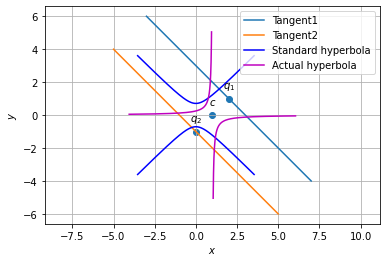
\includegraphics[width=\columnwidth]{./solutions/1/14/graph7.png}
	\caption{The standard and actual hyperbola.}
\end{figure}

\item $\begin{vmatrix}2&7&65\\3&8&75\\5&9&86\end{vmatrix}=0$
\\
\solution 
The given curve 
\begin{align}
	y =\frac{1}{x-1}
\end{align}
can be expressed as 
\begin{align}
	xy - y - 1 = 0 \label{eq:solutions/1/14/eq:hyperbola}
\end{align}
Hence, we have
\begin{align}
	\vec{V} = \frac{1}{2}\myvec{0 & 1 \\ 1 & 0}, 
	\vec{u} = \frac{1}{2}\myvec{0 \\-1},
	f = -1
\end{align}
Since $\mydet{\vec{V}} < 0$, the equation \eqref{eq:solutions/1/14/eq:hyperbola} represents hyperbola.
To find the values of $\lambda_1$ and $\lambda_2$, consider the characteristic equation,
\begin{align}
	\mydet{\lambda\vec{I} - \vec{V}} &= 0\\
	\implies \mydet{\myvec{\lambda & 0\\0 & \lambda} - \myvec{0 & \frac{1}{2} \\ \frac{1}{2} & 0}} &= 0\\
	\implies \mydet{ \lambda & \frac{-1}{2} \\ \frac{-1}{2} & \lambda} &= 0\\
	\implies \lambda_1 &= \frac{1}{2} , \lambda_2 = \frac{-1}{2}
\end{align}
In addition, given the slope -1, the direction and normal vectors are given by 
\begin{align}
	\vec{m} = \myvec{1 \\ -1} \\
	\vec{n} = \myvec{ 1 \\ 1}
\end{align}
The parameters of hyperbola are as follows:
\begin{align}
	\vec{c} &= -\vec{V}^{-1}\vec{u} \\
	&= -\myvec{0 & 2\\ 2 & 0}\myvec{0 \\ -\frac{1}{2}} \\
	&= \myvec{1 \\ 0}\\
	axes &= \begin{cases}
	\sqrt{\frac{\vec{u}^T\vec{V}^{-1}\vec{u} - f}{\lambda_1}} = \sqrt{2}\\
 \sqrt{\frac{f-\vec{u}^T\vec{V}^{-1}\vec{u}}{\lambda_2}} = \sqrt{2}
\end{cases}
\end{align}
which represents the standard hyperbola equation,
\begin{align}
	\frac{x^2}{2} - \frac{x^2}{2} = 1
\end{align}
The points of contact are given by 
\begin{align}
  \tiny{K} &=\pm \sqrt{\frac{\vec{u}^T\vec{V}^{-1}\vec{u} - f}{\vec{n}^T\vec{V}^{-1}\vec{n}}}
  = \pm \frac{1}{2}\\
  \vec{q} &= \vec{V}^{-1}(k\vec{n}-\vec{u})\\
  \vec{q_1} &= \myvec{0 & 2\\2 & 0} \sbrak{\frac{1}{2}\myvec{1 \\ 1} - \myvec{0\\ \frac{-1}{2}}}\\
  &= \myvec{2 \\ 1}\\
  \vec{q_2} &= \myvec{0 & 2\\2 & 0} \sbrak{\frac{-1}{2}\myvec{1 \\ 1} - \myvec{0\\ \frac{-1}{2}}}\\
  &= \myvec{0 \\ -1}
\end{align} 
$\therefore$ The tangents are given by
\begin{align}
	\myvec{1 & 1} \brak{\vec{x} - \myvec{2 \\ 1}} = 0 \\
	\myvec{1 & 1} \brak{\vec{x} - \myvec{0 \\ -1}} = 0
\end{align}
The desired equations of all lines having slope -1 that are tangents to the curve $\frac{1}{x-1}, x \neq 1$ are given by
\begin{align}
	\myvec{1 & 1}\vec{x} &= 3 \\
	\myvec{1 & 1}\vec{x} &= -1 
\end{align}
The above results are verified in the following figure.
\begin{figure}[h!] \label{eq:solutions/1/14/fig:tangents}
	\centering
	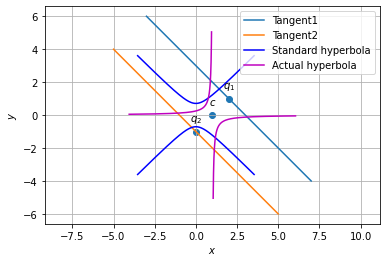
\includegraphics[width=\columnwidth]{./solutions/1/14/graph7.png}
	\caption{The standard and actual hyperbola.}
\end{figure}

\item $\begin{vmatrix}1&bc&a(b+c)\\1&ca&b(c+a)\\1&ab&c(a+b)\end{vmatrix}=0$
\\
\solution 
The given curve 
\begin{align}
	y =\frac{1}{x-1}
\end{align}
can be expressed as 
\begin{align}
	xy - y - 1 = 0 \label{eq:solutions/1/14/eq:hyperbola}
\end{align}
Hence, we have
\begin{align}
	\vec{V} = \frac{1}{2}\myvec{0 & 1 \\ 1 & 0}, 
	\vec{u} = \frac{1}{2}\myvec{0 \\-1},
	f = -1
\end{align}
Since $\mydet{\vec{V}} < 0$, the equation \eqref{eq:solutions/1/14/eq:hyperbola} represents hyperbola.
To find the values of $\lambda_1$ and $\lambda_2$, consider the characteristic equation,
\begin{align}
	\mydet{\lambda\vec{I} - \vec{V}} &= 0\\
	\implies \mydet{\myvec{\lambda & 0\\0 & \lambda} - \myvec{0 & \frac{1}{2} \\ \frac{1}{2} & 0}} &= 0\\
	\implies \mydet{ \lambda & \frac{-1}{2} \\ \frac{-1}{2} & \lambda} &= 0\\
	\implies \lambda_1 &= \frac{1}{2} , \lambda_2 = \frac{-1}{2}
\end{align}
In addition, given the slope -1, the direction and normal vectors are given by 
\begin{align}
	\vec{m} = \myvec{1 \\ -1} \\
	\vec{n} = \myvec{ 1 \\ 1}
\end{align}
The parameters of hyperbola are as follows:
\begin{align}
	\vec{c} &= -\vec{V}^{-1}\vec{u} \\
	&= -\myvec{0 & 2\\ 2 & 0}\myvec{0 \\ -\frac{1}{2}} \\
	&= \myvec{1 \\ 0}\\
	axes &= \begin{cases}
	\sqrt{\frac{\vec{u}^T\vec{V}^{-1}\vec{u} - f}{\lambda_1}} = \sqrt{2}\\
 \sqrt{\frac{f-\vec{u}^T\vec{V}^{-1}\vec{u}}{\lambda_2}} = \sqrt{2}
\end{cases}
\end{align}
which represents the standard hyperbola equation,
\begin{align}
	\frac{x^2}{2} - \frac{x^2}{2} = 1
\end{align}
The points of contact are given by 
\begin{align}
  \tiny{K} &=\pm \sqrt{\frac{\vec{u}^T\vec{V}^{-1}\vec{u} - f}{\vec{n}^T\vec{V}^{-1}\vec{n}}}
  = \pm \frac{1}{2}\\
  \vec{q} &= \vec{V}^{-1}(k\vec{n}-\vec{u})\\
  \vec{q_1} &= \myvec{0 & 2\\2 & 0} \sbrak{\frac{1}{2}\myvec{1 \\ 1} - \myvec{0\\ \frac{-1}{2}}}\\
  &= \myvec{2 \\ 1}\\
  \vec{q_2} &= \myvec{0 & 2\\2 & 0} \sbrak{\frac{-1}{2}\myvec{1 \\ 1} - \myvec{0\\ \frac{-1}{2}}}\\
  &= \myvec{0 \\ -1}
\end{align} 
$\therefore$ The tangents are given by
\begin{align}
	\myvec{1 & 1} \brak{\vec{x} - \myvec{2 \\ 1}} = 0 \\
	\myvec{1 & 1} \brak{\vec{x} - \myvec{0 \\ -1}} = 0
\end{align}
The desired equations of all lines having slope -1 that are tangents to the curve $\frac{1}{x-1}, x \neq 1$ are given by
\begin{align}
	\myvec{1 & 1}\vec{x} &= 3 \\
	\myvec{1 & 1}\vec{x} &= -1 
\end{align}
The above results are verified in the following figure.
\begin{figure}[h!] \label{eq:solutions/1/14/fig:tangents}
	\centering
	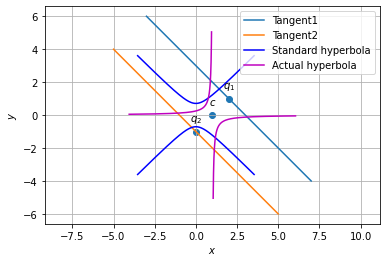
\includegraphics[width=\columnwidth]{./solutions/1/14/graph7.png}
	\caption{The standard and actual hyperbola.}
\end{figure}

\item $\begin{vmatrix}b+c& q+r& y+z\\c+a& r+p& z+x\\a+b& p+q& x+y\end{vmatrix}$=2$\begin{vmatrix} a&p&x\\b&q&y\\c&r&z\end{vmatrix}$ 
\\
\solution 
The given curve 
\begin{align}
	y =\frac{1}{x-1}
\end{align}
can be expressed as 
\begin{align}
	xy - y - 1 = 0 \label{eq:solutions/1/14/eq:hyperbola}
\end{align}
Hence, we have
\begin{align}
	\vec{V} = \frac{1}{2}\myvec{0 & 1 \\ 1 & 0}, 
	\vec{u} = \frac{1}{2}\myvec{0 \\-1},
	f = -1
\end{align}
Since $\mydet{\vec{V}} < 0$, the equation \eqref{eq:solutions/1/14/eq:hyperbola} represents hyperbola.
To find the values of $\lambda_1$ and $\lambda_2$, consider the characteristic equation,
\begin{align}
	\mydet{\lambda\vec{I} - \vec{V}} &= 0\\
	\implies \mydet{\myvec{\lambda & 0\\0 & \lambda} - \myvec{0 & \frac{1}{2} \\ \frac{1}{2} & 0}} &= 0\\
	\implies \mydet{ \lambda & \frac{-1}{2} \\ \frac{-1}{2} & \lambda} &= 0\\
	\implies \lambda_1 &= \frac{1}{2} , \lambda_2 = \frac{-1}{2}
\end{align}
In addition, given the slope -1, the direction and normal vectors are given by 
\begin{align}
	\vec{m} = \myvec{1 \\ -1} \\
	\vec{n} = \myvec{ 1 \\ 1}
\end{align}
The parameters of hyperbola are as follows:
\begin{align}
	\vec{c} &= -\vec{V}^{-1}\vec{u} \\
	&= -\myvec{0 & 2\\ 2 & 0}\myvec{0 \\ -\frac{1}{2}} \\
	&= \myvec{1 \\ 0}\\
	axes &= \begin{cases}
	\sqrt{\frac{\vec{u}^T\vec{V}^{-1}\vec{u} - f}{\lambda_1}} = \sqrt{2}\\
 \sqrt{\frac{f-\vec{u}^T\vec{V}^{-1}\vec{u}}{\lambda_2}} = \sqrt{2}
\end{cases}
\end{align}
which represents the standard hyperbola equation,
\begin{align}
	\frac{x^2}{2} - \frac{x^2}{2} = 1
\end{align}
The points of contact are given by 
\begin{align}
  \tiny{K} &=\pm \sqrt{\frac{\vec{u}^T\vec{V}^{-1}\vec{u} - f}{\vec{n}^T\vec{V}^{-1}\vec{n}}}
  = \pm \frac{1}{2}\\
  \vec{q} &= \vec{V}^{-1}(k\vec{n}-\vec{u})\\
  \vec{q_1} &= \myvec{0 & 2\\2 & 0} \sbrak{\frac{1}{2}\myvec{1 \\ 1} - \myvec{0\\ \frac{-1}{2}}}\\
  &= \myvec{2 \\ 1}\\
  \vec{q_2} &= \myvec{0 & 2\\2 & 0} \sbrak{\frac{-1}{2}\myvec{1 \\ 1} - \myvec{0\\ \frac{-1}{2}}}\\
  &= \myvec{0 \\ -1}
\end{align} 
$\therefore$ The tangents are given by
\begin{align}
	\myvec{1 & 1} \brak{\vec{x} - \myvec{2 \\ 1}} = 0 \\
	\myvec{1 & 1} \brak{\vec{x} - \myvec{0 \\ -1}} = 0
\end{align}
The desired equations of all lines having slope -1 that are tangents to the curve $\frac{1}{x-1}, x \neq 1$ are given by
\begin{align}
	\myvec{1 & 1}\vec{x} &= 3 \\
	\myvec{1 & 1}\vec{x} &= -1 
\end{align}
The above results are verified in the following figure.
\begin{figure}[h!] \label{eq:solutions/1/14/fig:tangents}
	\centering
	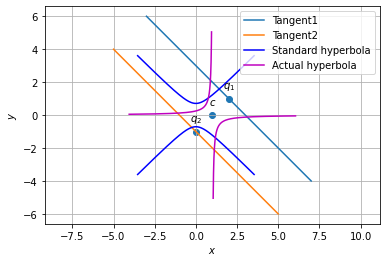
\includegraphics[width=\columnwidth]{./solutions/1/14/graph7.png}
	\caption{The standard and actual hyperbola.}
\end{figure}

\item $\begin{vmatrix}-a^2&ab&ab\\ ba&-b^2&bc\\ ca&cb&-c^2\end{vmatrix}$=$4a^2b^2c^2$\\
\\
\solution 
The given curve 
\begin{align}
	y =\frac{1}{x-1}
\end{align}
can be expressed as 
\begin{align}
	xy - y - 1 = 0 \label{eq:solutions/1/14/eq:hyperbola}
\end{align}
Hence, we have
\begin{align}
	\vec{V} = \frac{1}{2}\myvec{0 & 1 \\ 1 & 0}, 
	\vec{u} = \frac{1}{2}\myvec{0 \\-1},
	f = -1
\end{align}
Since $\mydet{\vec{V}} < 0$, the equation \eqref{eq:solutions/1/14/eq:hyperbola} represents hyperbola.
To find the values of $\lambda_1$ and $\lambda_2$, consider the characteristic equation,
\begin{align}
	\mydet{\lambda\vec{I} - \vec{V}} &= 0\\
	\implies \mydet{\myvec{\lambda & 0\\0 & \lambda} - \myvec{0 & \frac{1}{2} \\ \frac{1}{2} & 0}} &= 0\\
	\implies \mydet{ \lambda & \frac{-1}{2} \\ \frac{-1}{2} & \lambda} &= 0\\
	\implies \lambda_1 &= \frac{1}{2} , \lambda_2 = \frac{-1}{2}
\end{align}
In addition, given the slope -1, the direction and normal vectors are given by 
\begin{align}
	\vec{m} = \myvec{1 \\ -1} \\
	\vec{n} = \myvec{ 1 \\ 1}
\end{align}
The parameters of hyperbola are as follows:
\begin{align}
	\vec{c} &= -\vec{V}^{-1}\vec{u} \\
	&= -\myvec{0 & 2\\ 2 & 0}\myvec{0 \\ -\frac{1}{2}} \\
	&= \myvec{1 \\ 0}\\
	axes &= \begin{cases}
	\sqrt{\frac{\vec{u}^T\vec{V}^{-1}\vec{u} - f}{\lambda_1}} = \sqrt{2}\\
 \sqrt{\frac{f-\vec{u}^T\vec{V}^{-1}\vec{u}}{\lambda_2}} = \sqrt{2}
\end{cases}
\end{align}
which represents the standard hyperbola equation,
\begin{align}
	\frac{x^2}{2} - \frac{x^2}{2} = 1
\end{align}
The points of contact are given by 
\begin{align}
  \tiny{K} &=\pm \sqrt{\frac{\vec{u}^T\vec{V}^{-1}\vec{u} - f}{\vec{n}^T\vec{V}^{-1}\vec{n}}}
  = \pm \frac{1}{2}\\
  \vec{q} &= \vec{V}^{-1}(k\vec{n}-\vec{u})\\
  \vec{q_1} &= \myvec{0 & 2\\2 & 0} \sbrak{\frac{1}{2}\myvec{1 \\ 1} - \myvec{0\\ \frac{-1}{2}}}\\
  &= \myvec{2 \\ 1}\\
  \vec{q_2} &= \myvec{0 & 2\\2 & 0} \sbrak{\frac{-1}{2}\myvec{1 \\ 1} - \myvec{0\\ \frac{-1}{2}}}\\
  &= \myvec{0 \\ -1}
\end{align} 
$\therefore$ The tangents are given by
\begin{align}
	\myvec{1 & 1} \brak{\vec{x} - \myvec{2 \\ 1}} = 0 \\
	\myvec{1 & 1} \brak{\vec{x} - \myvec{0 \\ -1}} = 0
\end{align}
The desired equations of all lines having slope -1 that are tangents to the curve $\frac{1}{x-1}, x \neq 1$ are given by
\begin{align}
	\myvec{1 & 1}\vec{x} &= 3 \\
	\myvec{1 & 1}\vec{x} &= -1 
\end{align}
The above results are verified in the following figure.
\begin{figure}[h!] \label{eq:solutions/1/14/fig:tangents}
	\centering
	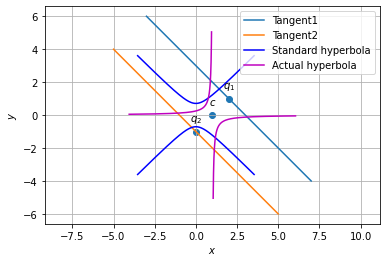
\includegraphics[width=\columnwidth]{./solutions/1/14/graph7.png}
	\caption{The standard and actual hyperbola.}
\end{figure}

By Using properties of determinants, in Exercises 16 to 22,Show that;
\item (i)$\begin{vmatrix}1&a&a^2\\1&b&b^2\\1&c&c^2\end{vmatrix}$=(a-b)(b-c)(c-a)\\
(ii) $\begin{vmatrix}1&1&1 \\ a&b&c \\ a^3&b^3&c^3\end{vmatrix}$=(a-b)(b-c)(c-a)(a+b+c)
\\
\solution 
The given curve 
\begin{align}
	y =\frac{1}{x-1}
\end{align}
can be expressed as 
\begin{align}
	xy - y - 1 = 0 \label{eq:solutions/1/14/eq:hyperbola}
\end{align}
Hence, we have
\begin{align}
	\vec{V} = \frac{1}{2}\myvec{0 & 1 \\ 1 & 0}, 
	\vec{u} = \frac{1}{2}\myvec{0 \\-1},
	f = -1
\end{align}
Since $\mydet{\vec{V}} < 0$, the equation \eqref{eq:solutions/1/14/eq:hyperbola} represents hyperbola.
To find the values of $\lambda_1$ and $\lambda_2$, consider the characteristic equation,
\begin{align}
	\mydet{\lambda\vec{I} - \vec{V}} &= 0\\
	\implies \mydet{\myvec{\lambda & 0\\0 & \lambda} - \myvec{0 & \frac{1}{2} \\ \frac{1}{2} & 0}} &= 0\\
	\implies \mydet{ \lambda & \frac{-1}{2} \\ \frac{-1}{2} & \lambda} &= 0\\
	\implies \lambda_1 &= \frac{1}{2} , \lambda_2 = \frac{-1}{2}
\end{align}
In addition, given the slope -1, the direction and normal vectors are given by 
\begin{align}
	\vec{m} = \myvec{1 \\ -1} \\
	\vec{n} = \myvec{ 1 \\ 1}
\end{align}
The parameters of hyperbola are as follows:
\begin{align}
	\vec{c} &= -\vec{V}^{-1}\vec{u} \\
	&= -\myvec{0 & 2\\ 2 & 0}\myvec{0 \\ -\frac{1}{2}} \\
	&= \myvec{1 \\ 0}\\
	axes &= \begin{cases}
	\sqrt{\frac{\vec{u}^T\vec{V}^{-1}\vec{u} - f}{\lambda_1}} = \sqrt{2}\\
 \sqrt{\frac{f-\vec{u}^T\vec{V}^{-1}\vec{u}}{\lambda_2}} = \sqrt{2}
\end{cases}
\end{align}
which represents the standard hyperbola equation,
\begin{align}
	\frac{x^2}{2} - \frac{x^2}{2} = 1
\end{align}
The points of contact are given by 
\begin{align}
  \tiny{K} &=\pm \sqrt{\frac{\vec{u}^T\vec{V}^{-1}\vec{u} - f}{\vec{n}^T\vec{V}^{-1}\vec{n}}}
  = \pm \frac{1}{2}\\
  \vec{q} &= \vec{V}^{-1}(k\vec{n}-\vec{u})\\
  \vec{q_1} &= \myvec{0 & 2\\2 & 0} \sbrak{\frac{1}{2}\myvec{1 \\ 1} - \myvec{0\\ \frac{-1}{2}}}\\
  &= \myvec{2 \\ 1}\\
  \vec{q_2} &= \myvec{0 & 2\\2 & 0} \sbrak{\frac{-1}{2}\myvec{1 \\ 1} - \myvec{0\\ \frac{-1}{2}}}\\
  &= \myvec{0 \\ -1}
\end{align} 
$\therefore$ The tangents are given by
\begin{align}
	\myvec{1 & 1} \brak{\vec{x} - \myvec{2 \\ 1}} = 0 \\
	\myvec{1 & 1} \brak{\vec{x} - \myvec{0 \\ -1}} = 0
\end{align}
The desired equations of all lines having slope -1 that are tangents to the curve $\frac{1}{x-1}, x \neq 1$ are given by
\begin{align}
	\myvec{1 & 1}\vec{x} &= 3 \\
	\myvec{1 & 1}\vec{x} &= -1 
\end{align}
The above results are verified in the following figure.
\begin{figure}[h!] \label{eq:solutions/1/14/fig:tangents}
	\centering
	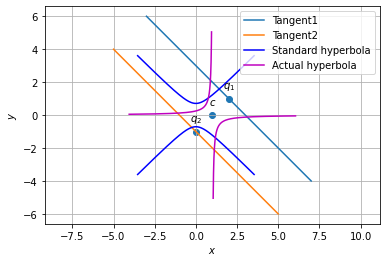
\includegraphics[width=\columnwidth]{./solutions/1/14/graph7.png}
	\caption{The standard and actual hyperbola.}
\end{figure}

\item $\begin{vmatrix}x&x^2&yz \\ y&y^2&zx \\ z&z^2&xy\end{vmatrix}$=(x-y)(y-z)(z-x)(xy+yz+zx)
\item (i) $\begin{vmatrix}x+4&2x&2x \\ 2x&x+4&2x \\ 2x&2x&x+4\end{vmatrix}$=$(5x+4)(4-x)^2$\\
\solution 
The given curve 
\begin{align}
	y =\frac{1}{x-1}
\end{align}
can be expressed as 
\begin{align}
	xy - y - 1 = 0 \label{eq:solutions/1/14/eq:hyperbola}
\end{align}
Hence, we have
\begin{align}
	\vec{V} = \frac{1}{2}\myvec{0 & 1 \\ 1 & 0}, 
	\vec{u} = \frac{1}{2}\myvec{0 \\-1},
	f = -1
\end{align}
Since $\mydet{\vec{V}} < 0$, the equation \eqref{eq:solutions/1/14/eq:hyperbola} represents hyperbola.
To find the values of $\lambda_1$ and $\lambda_2$, consider the characteristic equation,
\begin{align}
	\mydet{\lambda\vec{I} - \vec{V}} &= 0\\
	\implies \mydet{\myvec{\lambda & 0\\0 & \lambda} - \myvec{0 & \frac{1}{2} \\ \frac{1}{2} & 0}} &= 0\\
	\implies \mydet{ \lambda & \frac{-1}{2} \\ \frac{-1}{2} & \lambda} &= 0\\
	\implies \lambda_1 &= \frac{1}{2} , \lambda_2 = \frac{-1}{2}
\end{align}
In addition, given the slope -1, the direction and normal vectors are given by 
\begin{align}
	\vec{m} = \myvec{1 \\ -1} \\
	\vec{n} = \myvec{ 1 \\ 1}
\end{align}
The parameters of hyperbola are as follows:
\begin{align}
	\vec{c} &= -\vec{V}^{-1}\vec{u} \\
	&= -\myvec{0 & 2\\ 2 & 0}\myvec{0 \\ -\frac{1}{2}} \\
	&= \myvec{1 \\ 0}\\
	axes &= \begin{cases}
	\sqrt{\frac{\vec{u}^T\vec{V}^{-1}\vec{u} - f}{\lambda_1}} = \sqrt{2}\\
 \sqrt{\frac{f-\vec{u}^T\vec{V}^{-1}\vec{u}}{\lambda_2}} = \sqrt{2}
\end{cases}
\end{align}
which represents the standard hyperbola equation,
\begin{align}
	\frac{x^2}{2} - \frac{x^2}{2} = 1
\end{align}
The points of contact are given by 
\begin{align}
  \tiny{K} &=\pm \sqrt{\frac{\vec{u}^T\vec{V}^{-1}\vec{u} - f}{\vec{n}^T\vec{V}^{-1}\vec{n}}}
  = \pm \frac{1}{2}\\
  \vec{q} &= \vec{V}^{-1}(k\vec{n}-\vec{u})\\
  \vec{q_1} &= \myvec{0 & 2\\2 & 0} \sbrak{\frac{1}{2}\myvec{1 \\ 1} - \myvec{0\\ \frac{-1}{2}}}\\
  &= \myvec{2 \\ 1}\\
  \vec{q_2} &= \myvec{0 & 2\\2 & 0} \sbrak{\frac{-1}{2}\myvec{1 \\ 1} - \myvec{0\\ \frac{-1}{2}}}\\
  &= \myvec{0 \\ -1}
\end{align} 
$\therefore$ The tangents are given by
\begin{align}
	\myvec{1 & 1} \brak{\vec{x} - \myvec{2 \\ 1}} = 0 \\
	\myvec{1 & 1} \brak{\vec{x} - \myvec{0 \\ -1}} = 0
\end{align}
The desired equations of all lines having slope -1 that are tangents to the curve $\frac{1}{x-1}, x \neq 1$ are given by
\begin{align}
	\myvec{1 & 1}\vec{x} &= 3 \\
	\myvec{1 & 1}\vec{x} &= -1 
\end{align}
The above results are verified in the following figure.
\begin{figure}[h!] \label{eq:solutions/1/14/fig:tangents}
	\centering
	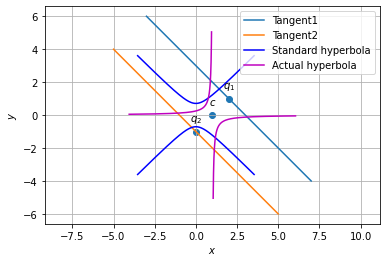
\includegraphics[width=\columnwidth]{./solutions/1/14/graph7.png}
	\caption{The standard and actual hyperbola.}
\end{figure}

(ii) $\begin{vmatrix}y+k&y&y \\ y&y+k&y \\ y&y&xy+k\end{vmatrix}$=$k^2(3y+k)$
\\
\solution 
The given curve 
\begin{align}
	y =\frac{1}{x-1}
\end{align}
can be expressed as 
\begin{align}
	xy - y - 1 = 0 \label{eq:solutions/1/14/eq:hyperbola}
\end{align}
Hence, we have
\begin{align}
	\vec{V} = \frac{1}{2}\myvec{0 & 1 \\ 1 & 0}, 
	\vec{u} = \frac{1}{2}\myvec{0 \\-1},
	f = -1
\end{align}
Since $\mydet{\vec{V}} < 0$, the equation \eqref{eq:solutions/1/14/eq:hyperbola} represents hyperbola.
To find the values of $\lambda_1$ and $\lambda_2$, consider the characteristic equation,
\begin{align}
	\mydet{\lambda\vec{I} - \vec{V}} &= 0\\
	\implies \mydet{\myvec{\lambda & 0\\0 & \lambda} - \myvec{0 & \frac{1}{2} \\ \frac{1}{2} & 0}} &= 0\\
	\implies \mydet{ \lambda & \frac{-1}{2} \\ \frac{-1}{2} & \lambda} &= 0\\
	\implies \lambda_1 &= \frac{1}{2} , \lambda_2 = \frac{-1}{2}
\end{align}
In addition, given the slope -1, the direction and normal vectors are given by 
\begin{align}
	\vec{m} = \myvec{1 \\ -1} \\
	\vec{n} = \myvec{ 1 \\ 1}
\end{align}
The parameters of hyperbola are as follows:
\begin{align}
	\vec{c} &= -\vec{V}^{-1}\vec{u} \\
	&= -\myvec{0 & 2\\ 2 & 0}\myvec{0 \\ -\frac{1}{2}} \\
	&= \myvec{1 \\ 0}\\
	axes &= \begin{cases}
	\sqrt{\frac{\vec{u}^T\vec{V}^{-1}\vec{u} - f}{\lambda_1}} = \sqrt{2}\\
 \sqrt{\frac{f-\vec{u}^T\vec{V}^{-1}\vec{u}}{\lambda_2}} = \sqrt{2}
\end{cases}
\end{align}
which represents the standard hyperbola equation,
\begin{align}
	\frac{x^2}{2} - \frac{x^2}{2} = 1
\end{align}
The points of contact are given by 
\begin{align}
  \tiny{K} &=\pm \sqrt{\frac{\vec{u}^T\vec{V}^{-1}\vec{u} - f}{\vec{n}^T\vec{V}^{-1}\vec{n}}}
  = \pm \frac{1}{2}\\
  \vec{q} &= \vec{V}^{-1}(k\vec{n}-\vec{u})\\
  \vec{q_1} &= \myvec{0 & 2\\2 & 0} \sbrak{\frac{1}{2}\myvec{1 \\ 1} - \myvec{0\\ \frac{-1}{2}}}\\
  &= \myvec{2 \\ 1}\\
  \vec{q_2} &= \myvec{0 & 2\\2 & 0} \sbrak{\frac{-1}{2}\myvec{1 \\ 1} - \myvec{0\\ \frac{-1}{2}}}\\
  &= \myvec{0 \\ -1}
\end{align} 
$\therefore$ The tangents are given by
\begin{align}
	\myvec{1 & 1} \brak{\vec{x} - \myvec{2 \\ 1}} = 0 \\
	\myvec{1 & 1} \brak{\vec{x} - \myvec{0 \\ -1}} = 0
\end{align}
The desired equations of all lines having slope -1 that are tangents to the curve $\frac{1}{x-1}, x \neq 1$ are given by
\begin{align}
	\myvec{1 & 1}\vec{x} &= 3 \\
	\myvec{1 & 1}\vec{x} &= -1 
\end{align}
The above results are verified in the following figure.
\begin{figure}[h!] \label{eq:solutions/1/14/fig:tangents}
	\centering
	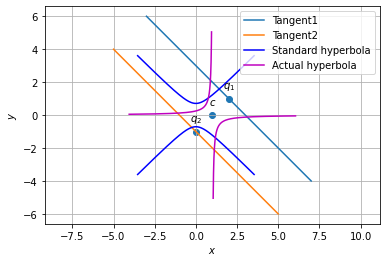
\includegraphics[width=\columnwidth]{./solutions/1/14/graph7.png}
	\caption{The standard and actual hyperbola.}
\end{figure}


\item $\begin{vmatrix}a^2+1&ab&ac \\ ab&b^2+1&bc \\ ca&cb&c^2+1\end{vmatrix}$=$1+a^2+b^2+c^2$\\
\\
\solution 
The given curve 
\begin{align}
	y =\frac{1}{x-1}
\end{align}
can be expressed as 
\begin{align}
	xy - y - 1 = 0 \label{eq:solutions/1/14/eq:hyperbola}
\end{align}
Hence, we have
\begin{align}
	\vec{V} = \frac{1}{2}\myvec{0 & 1 \\ 1 & 0}, 
	\vec{u} = \frac{1}{2}\myvec{0 \\-1},
	f = -1
\end{align}
Since $\mydet{\vec{V}} < 0$, the equation \eqref{eq:solutions/1/14/eq:hyperbola} represents hyperbola.
To find the values of $\lambda_1$ and $\lambda_2$, consider the characteristic equation,
\begin{align}
	\mydet{\lambda\vec{I} - \vec{V}} &= 0\\
	\implies \mydet{\myvec{\lambda & 0\\0 & \lambda} - \myvec{0 & \frac{1}{2} \\ \frac{1}{2} & 0}} &= 0\\
	\implies \mydet{ \lambda & \frac{-1}{2} \\ \frac{-1}{2} & \lambda} &= 0\\
	\implies \lambda_1 &= \frac{1}{2} , \lambda_2 = \frac{-1}{2}
\end{align}
In addition, given the slope -1, the direction and normal vectors are given by 
\begin{align}
	\vec{m} = \myvec{1 \\ -1} \\
	\vec{n} = \myvec{ 1 \\ 1}
\end{align}
The parameters of hyperbola are as follows:
\begin{align}
	\vec{c} &= -\vec{V}^{-1}\vec{u} \\
	&= -\myvec{0 & 2\\ 2 & 0}\myvec{0 \\ -\frac{1}{2}} \\
	&= \myvec{1 \\ 0}\\
	axes &= \begin{cases}
	\sqrt{\frac{\vec{u}^T\vec{V}^{-1}\vec{u} - f}{\lambda_1}} = \sqrt{2}\\
 \sqrt{\frac{f-\vec{u}^T\vec{V}^{-1}\vec{u}}{\lambda_2}} = \sqrt{2}
\end{cases}
\end{align}
which represents the standard hyperbola equation,
\begin{align}
	\frac{x^2}{2} - \frac{x^2}{2} = 1
\end{align}
The points of contact are given by 
\begin{align}
  \tiny{K} &=\pm \sqrt{\frac{\vec{u}^T\vec{V}^{-1}\vec{u} - f}{\vec{n}^T\vec{V}^{-1}\vec{n}}}
  = \pm \frac{1}{2}\\
  \vec{q} &= \vec{V}^{-1}(k\vec{n}-\vec{u})\\
  \vec{q_1} &= \myvec{0 & 2\\2 & 0} \sbrak{\frac{1}{2}\myvec{1 \\ 1} - \myvec{0\\ \frac{-1}{2}}}\\
  &= \myvec{2 \\ 1}\\
  \vec{q_2} &= \myvec{0 & 2\\2 & 0} \sbrak{\frac{-1}{2}\myvec{1 \\ 1} - \myvec{0\\ \frac{-1}{2}}}\\
  &= \myvec{0 \\ -1}
\end{align} 
$\therefore$ The tangents are given by
\begin{align}
	\myvec{1 & 1} \brak{\vec{x} - \myvec{2 \\ 1}} = 0 \\
	\myvec{1 & 1} \brak{\vec{x} - \myvec{0 \\ -1}} = 0
\end{align}
The desired equations of all lines having slope -1 that are tangents to the curve $\frac{1}{x-1}, x \neq 1$ are given by
\begin{align}
	\myvec{1 & 1}\vec{x} &= 3 \\
	\myvec{1 & 1}\vec{x} &= -1 
\end{align}
The above results are verified in the following figure.
\begin{figure}[h!] \label{eq:solutions/1/14/fig:tangents}
	\centering
	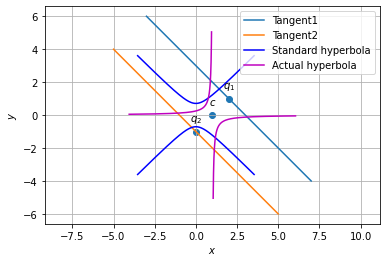
\includegraphics[width=\columnwidth]{./solutions/1/14/graph7.png}
	\caption{The standard and actual hyperbola.}
\end{figure}

Choose the correct answer in Exercises 23 and 24.
\item Let A be a square matrix of order 3X3, then 
$\abs{kA}$ is equal to
\begin{enumerate}
\item $k\abs{A}$
\item $k^2\abs{A}$
\item $k^3\abs{A}$
\item $3k\abs{A}$
\end{enumerate} 
\item Which of the following is correct
\begin{enumerate}
\item Determinant is a square matrix.
\item Determinant is a number associated to a matrix.
\item Determinant is a number associated to a square matrix.
\item None of these.
\end{enumerate}
\item Find area of the triangle with vertices at the point given in each of the following :\\
(i) \myvec{1&0}, \myvec{6&0}, \myvec{4&3}\\
(ii) \myvec{2&7}, \myvec{1&1}, \myvec{10&8}\\
(iii) \myvec{-2&-3}, \myvec{3&2}, \myvec{-1&-8}\\
\item Show that points A=\myvec{a&b+c}, B=\myvec{b&c+a}, C=\myvec{c&a+b} are collinear.
\\
\solution 
The given curve 
\begin{align}
	y =\frac{1}{x-1}
\end{align}
can be expressed as 
\begin{align}
	xy - y - 1 = 0 \label{eq:solutions/1/14/eq:hyperbola}
\end{align}
Hence, we have
\begin{align}
	\vec{V} = \frac{1}{2}\myvec{0 & 1 \\ 1 & 0}, 
	\vec{u} = \frac{1}{2}\myvec{0 \\-1},
	f = -1
\end{align}
Since $\mydet{\vec{V}} < 0$, the equation \eqref{eq:solutions/1/14/eq:hyperbola} represents hyperbola.
To find the values of $\lambda_1$ and $\lambda_2$, consider the characteristic equation,
\begin{align}
	\mydet{\lambda\vec{I} - \vec{V}} &= 0\\
	\implies \mydet{\myvec{\lambda & 0\\0 & \lambda} - \myvec{0 & \frac{1}{2} \\ \frac{1}{2} & 0}} &= 0\\
	\implies \mydet{ \lambda & \frac{-1}{2} \\ \frac{-1}{2} & \lambda} &= 0\\
	\implies \lambda_1 &= \frac{1}{2} , \lambda_2 = \frac{-1}{2}
\end{align}
In addition, given the slope -1, the direction and normal vectors are given by 
\begin{align}
	\vec{m} = \myvec{1 \\ -1} \\
	\vec{n} = \myvec{ 1 \\ 1}
\end{align}
The parameters of hyperbola are as follows:
\begin{align}
	\vec{c} &= -\vec{V}^{-1}\vec{u} \\
	&= -\myvec{0 & 2\\ 2 & 0}\myvec{0 \\ -\frac{1}{2}} \\
	&= \myvec{1 \\ 0}\\
	axes &= \begin{cases}
	\sqrt{\frac{\vec{u}^T\vec{V}^{-1}\vec{u} - f}{\lambda_1}} = \sqrt{2}\\
 \sqrt{\frac{f-\vec{u}^T\vec{V}^{-1}\vec{u}}{\lambda_2}} = \sqrt{2}
\end{cases}
\end{align}
which represents the standard hyperbola equation,
\begin{align}
	\frac{x^2}{2} - \frac{x^2}{2} = 1
\end{align}
The points of contact are given by 
\begin{align}
  \tiny{K} &=\pm \sqrt{\frac{\vec{u}^T\vec{V}^{-1}\vec{u} - f}{\vec{n}^T\vec{V}^{-1}\vec{n}}}
  = \pm \frac{1}{2}\\
  \vec{q} &= \vec{V}^{-1}(k\vec{n}-\vec{u})\\
  \vec{q_1} &= \myvec{0 & 2\\2 & 0} \sbrak{\frac{1}{2}\myvec{1 \\ 1} - \myvec{0\\ \frac{-1}{2}}}\\
  &= \myvec{2 \\ 1}\\
  \vec{q_2} &= \myvec{0 & 2\\2 & 0} \sbrak{\frac{-1}{2}\myvec{1 \\ 1} - \myvec{0\\ \frac{-1}{2}}}\\
  &= \myvec{0 \\ -1}
\end{align} 
$\therefore$ The tangents are given by
\begin{align}
	\myvec{1 & 1} \brak{\vec{x} - \myvec{2 \\ 1}} = 0 \\
	\myvec{1 & 1} \brak{\vec{x} - \myvec{0 \\ -1}} = 0
\end{align}
The desired equations of all lines having slope -1 that are tangents to the curve $\frac{1}{x-1}, x \neq 1$ are given by
\begin{align}
	\myvec{1 & 1}\vec{x} &= 3 \\
	\myvec{1 & 1}\vec{x} &= -1 
\end{align}
The above results are verified in the following figure.
\begin{figure}[h!] \label{eq:solutions/1/14/fig:tangents}
	\centering
	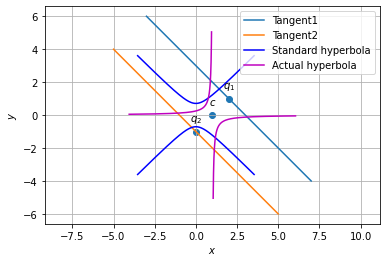
\includegraphics[width=\columnwidth]{./solutions/1/14/graph7.png}
	\caption{The standard and actual hyperbola.}
\end{figure}

\item Find values of k if area of triangle is 4sq.units and vertices are \\
(i) \myvec{k&0}, \myvec{4&0}, \myvec{0&2} \\ (ii) \myvec{-2&0}, \myvec{0&4}, \myvec{0&k}
\item (i) Find equation of line joining \myvec{1&2} and \myvec{3&6} using determinants.\\
(ii) Find equation of line joining \myvec{3&1} and \myvec{9&3} using determinants.
\item If the area of triangle is 35 sq.units with vertices \myvec{2&-6}, \myvec{5&4} and \myvec{k&4}.then k is 
\begin{enumerate}
\item 12
\item -2
\item -12,-2
\item 12,-2
\end{enumerate}

\textbf{Write Minors and Coafactors of the elements of following determinants:}
\item (i) $\begin{vmatrix}
2&-4 \\ 0 &3 \end{vmatrix}$ \\
(ii) $\begin{vmatrix}a&c \\ b &d\end{vmatrix}$
\item (i) $\begin{vmatrix}1&0&0 \\ 0&1&0 \\ 0&0&1\end{vmatrix}$\\
(ii) $\begin{vmatrix}1&0&4 \\ 3&5&-1 \\ 0&1&2\end{vmatrix}$
\item Using Cofactors of elements of second row,evaluate $\Delta$ =
$\begin{vmatrix} 5&3&8 \\ 2&0&1 \\ 1&2&3 \end{vmatrix}.$
\item Using Cofactors of elements of third column ,evaluate $\Delta$ = 
$\begin{vmatrix} 1&x&yz \\ 1&y&zx \\ 1&z&xy \end{vmatrix}.$
\item If $\Delta = \begin{vmatrix}
a_{11}&a_{12}&a_{13} \\ a_{21}&a_{22}&a_{23} \\ a_{31}&a_{32}&a_{33}
\end{vmatrix}$ and $A_{ij}$ is Cofactors of $a_{ij}$ then value of $\Delta$ is given by 
\begin{enumerate}
\item $a_{11}A_{31}+a_{12}A_{32}+a_{13}A_{33}$
\item $a_{11}A_{11}+a_{12}A_{21}+a_{13}A_{31}$
\item $a_{21}A_{11}+a_{22}A_{12}+a_{23}A_{13}$
\item $a_{11}A_{11}+a_{21}A_{21}+a_{31}A_{31}$
\end{enumerate} 
\textbf{Find adjoint of each of the matrices} 
\item $\begin{bmatrix}
1&2 \\ 3&4
\end{bmatrix}$
\item $\begin{bmatrix}
1&-1&2 \\ 2&3&5 \\ -2&0&1
\end{bmatrix}$
Verify A(adjA)=(adjA)A=$\abs{A}I$
\item $\begin{bmatrix}
2&3 \\ -4&-6
\end{bmatrix}$
\item $\begin{bmatrix}
1&-1&2 \\ 3&0&-2 \\ 1&0&3
\end{bmatrix}$
\item $\begin{bmatrix}
2&-2 \\ 4&3
\end{bmatrix}$
\item $\begin{bmatrix}
-1&5 \\ -3&2
\end{bmatrix}$
\item $\begin{bmatrix}
1&2&3 \\ 0&2&4 \\ 0&0&5
\end{bmatrix}$
\item $\begin{bmatrix}
1&0&0 \\ 3&3&0 \\ 5&2&-1
\end{bmatrix}$
\item $\begin{bmatrix}
2&1&3 \\ 4&-1&0 \\ -7&2&1
\end{bmatrix}$
\item $\begin{bmatrix}
1&-1&2 \\ 0&2&-3 \\ 3&-2&4
\end{bmatrix}$
\item $\begin{bmatrix}
1&0&0 \\ 0& \cos\alpha &\sin\alpha \\ 0&\sin\alpha&-\cos\alpha
\end{bmatrix}$
\item Let A=
$\begin{bmatrix}
3&7 \\ 2&5
\end{bmatrix}$ and B=
$\begin{bmatrix}
6&8 \\ 7&9
\end{bmatrix}.$ Verify that $(AB)^{-1}=B^{-1} A^{-1}$
\item Let A =$\begin{bmatrix}
3&1 \\ -1&2
\end{bmatrix},$ show that $A^2-5A+7I=O.$ Hence find $A^{-1}$
\solution 
The given curve 
\begin{align}
	y =\frac{1}{x-1}
\end{align}
can be expressed as 
\begin{align}
	xy - y - 1 = 0 \label{eq:solutions/1/14/eq:hyperbola}
\end{align}
Hence, we have
\begin{align}
	\vec{V} = \frac{1}{2}\myvec{0 & 1 \\ 1 & 0}, 
	\vec{u} = \frac{1}{2}\myvec{0 \\-1},
	f = -1
\end{align}
Since $\mydet{\vec{V}} < 0$, the equation \eqref{eq:solutions/1/14/eq:hyperbola} represents hyperbola.
To find the values of $\lambda_1$ and $\lambda_2$, consider the characteristic equation,
\begin{align}
	\mydet{\lambda\vec{I} - \vec{V}} &= 0\\
	\implies \mydet{\myvec{\lambda & 0\\0 & \lambda} - \myvec{0 & \frac{1}{2} \\ \frac{1}{2} & 0}} &= 0\\
	\implies \mydet{ \lambda & \frac{-1}{2} \\ \frac{-1}{2} & \lambda} &= 0\\
	\implies \lambda_1 &= \frac{1}{2} , \lambda_2 = \frac{-1}{2}
\end{align}
In addition, given the slope -1, the direction and normal vectors are given by 
\begin{align}
	\vec{m} = \myvec{1 \\ -1} \\
	\vec{n} = \myvec{ 1 \\ 1}
\end{align}
The parameters of hyperbola are as follows:
\begin{align}
	\vec{c} &= -\vec{V}^{-1}\vec{u} \\
	&= -\myvec{0 & 2\\ 2 & 0}\myvec{0 \\ -\frac{1}{2}} \\
	&= \myvec{1 \\ 0}\\
	axes &= \begin{cases}
	\sqrt{\frac{\vec{u}^T\vec{V}^{-1}\vec{u} - f}{\lambda_1}} = \sqrt{2}\\
 \sqrt{\frac{f-\vec{u}^T\vec{V}^{-1}\vec{u}}{\lambda_2}} = \sqrt{2}
\end{cases}
\end{align}
which represents the standard hyperbola equation,
\begin{align}
	\frac{x^2}{2} - \frac{x^2}{2} = 1
\end{align}
The points of contact are given by 
\begin{align}
  \tiny{K} &=\pm \sqrt{\frac{\vec{u}^T\vec{V}^{-1}\vec{u} - f}{\vec{n}^T\vec{V}^{-1}\vec{n}}}
  = \pm \frac{1}{2}\\
  \vec{q} &= \vec{V}^{-1}(k\vec{n}-\vec{u})\\
  \vec{q_1} &= \myvec{0 & 2\\2 & 0} \sbrak{\frac{1}{2}\myvec{1 \\ 1} - \myvec{0\\ \frac{-1}{2}}}\\
  &= \myvec{2 \\ 1}\\
  \vec{q_2} &= \myvec{0 & 2\\2 & 0} \sbrak{\frac{-1}{2}\myvec{1 \\ 1} - \myvec{0\\ \frac{-1}{2}}}\\
  &= \myvec{0 \\ -1}
\end{align} 
$\therefore$ The tangents are given by
\begin{align}
	\myvec{1 & 1} \brak{\vec{x} - \myvec{2 \\ 1}} = 0 \\
	\myvec{1 & 1} \brak{\vec{x} - \myvec{0 \\ -1}} = 0
\end{align}
The desired equations of all lines having slope -1 that are tangents to the curve $\frac{1}{x-1}, x \neq 1$ are given by
\begin{align}
	\myvec{1 & 1}\vec{x} &= 3 \\
	\myvec{1 & 1}\vec{x} &= -1 
\end{align}
The above results are verified in the following figure.
\begin{figure}[h!] \label{eq:solutions/1/14/fig:tangents}
	\centering
	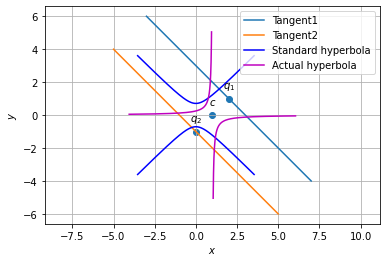
\includegraphics[width=\columnwidth]{./solutions/1/14/graph7.png}
	\caption{The standard and actual hyperbola.}
\end{figure}

\item For the matrix A= $\begin{bmatrix}
3&2 \\ 1&1
\end{bmatrix},$ find the numbers a and b such that $A^2+aA+bI=O.$
\\
\solution 
The given curve 
\begin{align}
	y =\frac{1}{x-1}
\end{align}
can be expressed as 
\begin{align}
	xy - y - 1 = 0 \label{eq:solutions/1/14/eq:hyperbola}
\end{align}
Hence, we have
\begin{align}
	\vec{V} = \frac{1}{2}\myvec{0 & 1 \\ 1 & 0}, 
	\vec{u} = \frac{1}{2}\myvec{0 \\-1},
	f = -1
\end{align}
Since $\mydet{\vec{V}} < 0$, the equation \eqref{eq:solutions/1/14/eq:hyperbola} represents hyperbola.
To find the values of $\lambda_1$ and $\lambda_2$, consider the characteristic equation,
\begin{align}
	\mydet{\lambda\vec{I} - \vec{V}} &= 0\\
	\implies \mydet{\myvec{\lambda & 0\\0 & \lambda} - \myvec{0 & \frac{1}{2} \\ \frac{1}{2} & 0}} &= 0\\
	\implies \mydet{ \lambda & \frac{-1}{2} \\ \frac{-1}{2} & \lambda} &= 0\\
	\implies \lambda_1 &= \frac{1}{2} , \lambda_2 = \frac{-1}{2}
\end{align}
In addition, given the slope -1, the direction and normal vectors are given by 
\begin{align}
	\vec{m} = \myvec{1 \\ -1} \\
	\vec{n} = \myvec{ 1 \\ 1}
\end{align}
The parameters of hyperbola are as follows:
\begin{align}
	\vec{c} &= -\vec{V}^{-1}\vec{u} \\
	&= -\myvec{0 & 2\\ 2 & 0}\myvec{0 \\ -\frac{1}{2}} \\
	&= \myvec{1 \\ 0}\\
	axes &= \begin{cases}
	\sqrt{\frac{\vec{u}^T\vec{V}^{-1}\vec{u} - f}{\lambda_1}} = \sqrt{2}\\
 \sqrt{\frac{f-\vec{u}^T\vec{V}^{-1}\vec{u}}{\lambda_2}} = \sqrt{2}
\end{cases}
\end{align}
which represents the standard hyperbola equation,
\begin{align}
	\frac{x^2}{2} - \frac{x^2}{2} = 1
\end{align}
The points of contact are given by 
\begin{align}
  \tiny{K} &=\pm \sqrt{\frac{\vec{u}^T\vec{V}^{-1}\vec{u} - f}{\vec{n}^T\vec{V}^{-1}\vec{n}}}
  = \pm \frac{1}{2}\\
  \vec{q} &= \vec{V}^{-1}(k\vec{n}-\vec{u})\\
  \vec{q_1} &= \myvec{0 & 2\\2 & 0} \sbrak{\frac{1}{2}\myvec{1 \\ 1} - \myvec{0\\ \frac{-1}{2}}}\\
  &= \myvec{2 \\ 1}\\
  \vec{q_2} &= \myvec{0 & 2\\2 & 0} \sbrak{\frac{-1}{2}\myvec{1 \\ 1} - \myvec{0\\ \frac{-1}{2}}}\\
  &= \myvec{0 \\ -1}
\end{align} 
$\therefore$ The tangents are given by
\begin{align}
	\myvec{1 & 1} \brak{\vec{x} - \myvec{2 \\ 1}} = 0 \\
	\myvec{1 & 1} \brak{\vec{x} - \myvec{0 \\ -1}} = 0
\end{align}
The desired equations of all lines having slope -1 that are tangents to the curve $\frac{1}{x-1}, x \neq 1$ are given by
\begin{align}
	\myvec{1 & 1}\vec{x} &= 3 \\
	\myvec{1 & 1}\vec{x} &= -1 
\end{align}
The above results are verified in the following figure.
\begin{figure}[h!] \label{eq:solutions/1/14/fig:tangents}
	\centering
	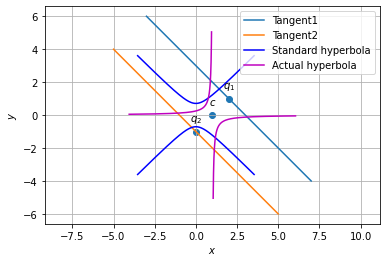
\includegraphics[width=\columnwidth]{./solutions/1/14/graph7.png}
	\caption{The standard and actual hyperbola.}
\end{figure}


\item For the matrix A=$\myvec{1&1&1 \\ 1&2&-3 \\ 2&-1&3}$.Show that \begin{align}
    A^3-6A^2+5A+11I=0\label{eq:det/49/1}
\end{align} and hence find $A^{-1}$.
%\item For the matrix A=$\begin{bmatrix}
%1&1&1 \\ 1&2&-3 \\ 2&-1&3
%\end{bmatrix}$ Show that $A^3-6A^2+9A-4I=O$ and hence find $A^{-1}$
\solution 
The given curve 
\begin{align}
	y =\frac{1}{x-1}
\end{align}
can be expressed as 
\begin{align}
	xy - y - 1 = 0 \label{eq:solutions/1/14/eq:hyperbola}
\end{align}
Hence, we have
\begin{align}
	\vec{V} = \frac{1}{2}\myvec{0 & 1 \\ 1 & 0}, 
	\vec{u} = \frac{1}{2}\myvec{0 \\-1},
	f = -1
\end{align}
Since $\mydet{\vec{V}} < 0$, the equation \eqref{eq:solutions/1/14/eq:hyperbola} represents hyperbola.
To find the values of $\lambda_1$ and $\lambda_2$, consider the characteristic equation,
\begin{align}
	\mydet{\lambda\vec{I} - \vec{V}} &= 0\\
	\implies \mydet{\myvec{\lambda & 0\\0 & \lambda} - \myvec{0 & \frac{1}{2} \\ \frac{1}{2} & 0}} &= 0\\
	\implies \mydet{ \lambda & \frac{-1}{2} \\ \frac{-1}{2} & \lambda} &= 0\\
	\implies \lambda_1 &= \frac{1}{2} , \lambda_2 = \frac{-1}{2}
\end{align}
In addition, given the slope -1, the direction and normal vectors are given by 
\begin{align}
	\vec{m} = \myvec{1 \\ -1} \\
	\vec{n} = \myvec{ 1 \\ 1}
\end{align}
The parameters of hyperbola are as follows:
\begin{align}
	\vec{c} &= -\vec{V}^{-1}\vec{u} \\
	&= -\myvec{0 & 2\\ 2 & 0}\myvec{0 \\ -\frac{1}{2}} \\
	&= \myvec{1 \\ 0}\\
	axes &= \begin{cases}
	\sqrt{\frac{\vec{u}^T\vec{V}^{-1}\vec{u} - f}{\lambda_1}} = \sqrt{2}\\
 \sqrt{\frac{f-\vec{u}^T\vec{V}^{-1}\vec{u}}{\lambda_2}} = \sqrt{2}
\end{cases}
\end{align}
which represents the standard hyperbola equation,
\begin{align}
	\frac{x^2}{2} - \frac{x^2}{2} = 1
\end{align}
The points of contact are given by 
\begin{align}
  \tiny{K} &=\pm \sqrt{\frac{\vec{u}^T\vec{V}^{-1}\vec{u} - f}{\vec{n}^T\vec{V}^{-1}\vec{n}}}
  = \pm \frac{1}{2}\\
  \vec{q} &= \vec{V}^{-1}(k\vec{n}-\vec{u})\\
  \vec{q_1} &= \myvec{0 & 2\\2 & 0} \sbrak{\frac{1}{2}\myvec{1 \\ 1} - \myvec{0\\ \frac{-1}{2}}}\\
  &= \myvec{2 \\ 1}\\
  \vec{q_2} &= \myvec{0 & 2\\2 & 0} \sbrak{\frac{-1}{2}\myvec{1 \\ 1} - \myvec{0\\ \frac{-1}{2}}}\\
  &= \myvec{0 \\ -1}
\end{align} 
$\therefore$ The tangents are given by
\begin{align}
	\myvec{1 & 1} \brak{\vec{x} - \myvec{2 \\ 1}} = 0 \\
	\myvec{1 & 1} \brak{\vec{x} - \myvec{0 \\ -1}} = 0
\end{align}
The desired equations of all lines having slope -1 that are tangents to the curve $\frac{1}{x-1}, x \neq 1$ are given by
\begin{align}
	\myvec{1 & 1}\vec{x} &= 3 \\
	\myvec{1 & 1}\vec{x} &= -1 
\end{align}
The above results are verified in the following figure.
\begin{figure}[h!] \label{eq:solutions/1/14/fig:tangents}
	\centering
	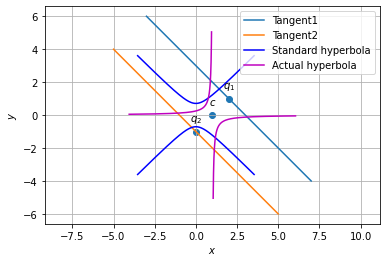
\includegraphics[width=\columnwidth]{./solutions/1/14/graph7.png}
	\caption{The standard and actual hyperbola.}
\end{figure}

\item Let A be a nonsingular square matrix of order 3X3 .Then $\abs{adjA}$ is equal to 
\begin{enumerate}
\item $\abs{A}$
\item $\abs{A}^2$
\item $\abs{A}^3$
\item $3\abs{A}$
\end{enumerate}
\item If A is an invertible matrix of order 2, then det($A^{-1}$) is equal to 
\begin{enumerate}
\item det(A)
\item $\frac{1}{det(A)}$
\item 1
\item 0
\end{enumerate}
\textbf{Examine the consistency of the system of given Equations.}
\item $\begin{alignedat}[t]{2}
x+3y&=5 
\\
2x+6y&=8 
\end{alignedat}$\\
\\
\solution 
The given curve 
\begin{align}
	y =\frac{1}{x-1}
\end{align}
can be expressed as 
\begin{align}
	xy - y - 1 = 0 \label{eq:solutions/1/14/eq:hyperbola}
\end{align}
Hence, we have
\begin{align}
	\vec{V} = \frac{1}{2}\myvec{0 & 1 \\ 1 & 0}, 
	\vec{u} = \frac{1}{2}\myvec{0 \\-1},
	f = -1
\end{align}
Since $\mydet{\vec{V}} < 0$, the equation \eqref{eq:solutions/1/14/eq:hyperbola} represents hyperbola.
To find the values of $\lambda_1$ and $\lambda_2$, consider the characteristic equation,
\begin{align}
	\mydet{\lambda\vec{I} - \vec{V}} &= 0\\
	\implies \mydet{\myvec{\lambda & 0\\0 & \lambda} - \myvec{0 & \frac{1}{2} \\ \frac{1}{2} & 0}} &= 0\\
	\implies \mydet{ \lambda & \frac{-1}{2} \\ \frac{-1}{2} & \lambda} &= 0\\
	\implies \lambda_1 &= \frac{1}{2} , \lambda_2 = \frac{-1}{2}
\end{align}
In addition, given the slope -1, the direction and normal vectors are given by 
\begin{align}
	\vec{m} = \myvec{1 \\ -1} \\
	\vec{n} = \myvec{ 1 \\ 1}
\end{align}
The parameters of hyperbola are as follows:
\begin{align}
	\vec{c} &= -\vec{V}^{-1}\vec{u} \\
	&= -\myvec{0 & 2\\ 2 & 0}\myvec{0 \\ -\frac{1}{2}} \\
	&= \myvec{1 \\ 0}\\
	axes &= \begin{cases}
	\sqrt{\frac{\vec{u}^T\vec{V}^{-1}\vec{u} - f}{\lambda_1}} = \sqrt{2}\\
 \sqrt{\frac{f-\vec{u}^T\vec{V}^{-1}\vec{u}}{\lambda_2}} = \sqrt{2}
\end{cases}
\end{align}
which represents the standard hyperbola equation,
\begin{align}
	\frac{x^2}{2} - \frac{x^2}{2} = 1
\end{align}
The points of contact are given by 
\begin{align}
  \tiny{K} &=\pm \sqrt{\frac{\vec{u}^T\vec{V}^{-1}\vec{u} - f}{\vec{n}^T\vec{V}^{-1}\vec{n}}}
  = \pm \frac{1}{2}\\
  \vec{q} &= \vec{V}^{-1}(k\vec{n}-\vec{u})\\
  \vec{q_1} &= \myvec{0 & 2\\2 & 0} \sbrak{\frac{1}{2}\myvec{1 \\ 1} - \myvec{0\\ \frac{-1}{2}}}\\
  &= \myvec{2 \\ 1}\\
  \vec{q_2} &= \myvec{0 & 2\\2 & 0} \sbrak{\frac{-1}{2}\myvec{1 \\ 1} - \myvec{0\\ \frac{-1}{2}}}\\
  &= \myvec{0 \\ -1}
\end{align} 
$\therefore$ The tangents are given by
\begin{align}
	\myvec{1 & 1} \brak{\vec{x} - \myvec{2 \\ 1}} = 0 \\
	\myvec{1 & 1} \brak{\vec{x} - \myvec{0 \\ -1}} = 0
\end{align}
The desired equations of all lines having slope -1 that are tangents to the curve $\frac{1}{x-1}, x \neq 1$ are given by
\begin{align}
	\myvec{1 & 1}\vec{x} &= 3 \\
	\myvec{1 & 1}\vec{x} &= -1 
\end{align}
The above results are verified in the following figure.
\begin{figure}[h!] \label{eq:solutions/1/14/fig:tangents}
	\centering
	\includegraphics[width=\columnwidth]{./solutions/1/14/graph7.png}
	\caption{The standard and actual hyperbola.}
\end{figure}

\item x+y+z=1\\ 2x+3y+2z=2\\ax+ay+2az=4\\
\\
\solution 
The given curve 
\begin{align}
	y =\frac{1}{x-1}
\end{align}
can be expressed as 
\begin{align}
	xy - y - 1 = 0 \label{eq:solutions/1/14/eq:hyperbola}
\end{align}
Hence, we have
\begin{align}
	\vec{V} = \frac{1}{2}\myvec{0 & 1 \\ 1 & 0}, 
	\vec{u} = \frac{1}{2}\myvec{0 \\-1},
	f = -1
\end{align}
Since $\mydet{\vec{V}} < 0$, the equation \eqref{eq:solutions/1/14/eq:hyperbola} represents hyperbola.
To find the values of $\lambda_1$ and $\lambda_2$, consider the characteristic equation,
\begin{align}
	\mydet{\lambda\vec{I} - \vec{V}} &= 0\\
	\implies \mydet{\myvec{\lambda & 0\\0 & \lambda} - \myvec{0 & \frac{1}{2} \\ \frac{1}{2} & 0}} &= 0\\
	\implies \mydet{ \lambda & \frac{-1}{2} \\ \frac{-1}{2} & \lambda} &= 0\\
	\implies \lambda_1 &= \frac{1}{2} , \lambda_2 = \frac{-1}{2}
\end{align}
In addition, given the slope -1, the direction and normal vectors are given by 
\begin{align}
	\vec{m} = \myvec{1 \\ -1} \\
	\vec{n} = \myvec{ 1 \\ 1}
\end{align}
The parameters of hyperbola are as follows:
\begin{align}
	\vec{c} &= -\vec{V}^{-1}\vec{u} \\
	&= -\myvec{0 & 2\\ 2 & 0}\myvec{0 \\ -\frac{1}{2}} \\
	&= \myvec{1 \\ 0}\\
	axes &= \begin{cases}
	\sqrt{\frac{\vec{u}^T\vec{V}^{-1}\vec{u} - f}{\lambda_1}} = \sqrt{2}\\
 \sqrt{\frac{f-\vec{u}^T\vec{V}^{-1}\vec{u}}{\lambda_2}} = \sqrt{2}
\end{cases}
\end{align}
which represents the standard hyperbola equation,
\begin{align}
	\frac{x^2}{2} - \frac{x^2}{2} = 1
\end{align}
The points of contact are given by 
\begin{align}
  \tiny{K} &=\pm \sqrt{\frac{\vec{u}^T\vec{V}^{-1}\vec{u} - f}{\vec{n}^T\vec{V}^{-1}\vec{n}}}
  = \pm \frac{1}{2}\\
  \vec{q} &= \vec{V}^{-1}(k\vec{n}-\vec{u})\\
  \vec{q_1} &= \myvec{0 & 2\\2 & 0} \sbrak{\frac{1}{2}\myvec{1 \\ 1} - \myvec{0\\ \frac{-1}{2}}}\\
  &= \myvec{2 \\ 1}\\
  \vec{q_2} &= \myvec{0 & 2\\2 & 0} \sbrak{\frac{-1}{2}\myvec{1 \\ 1} - \myvec{0\\ \frac{-1}{2}}}\\
  &= \myvec{0 \\ -1}
\end{align} 
$\therefore$ The tangents are given by
\begin{align}
	\myvec{1 & 1} \brak{\vec{x} - \myvec{2 \\ 1}} = 0 \\
	\myvec{1 & 1} \brak{\vec{x} - \myvec{0 \\ -1}} = 0
\end{align}
The desired equations of all lines having slope -1 that are tangents to the curve $\frac{1}{x-1}, x \neq 1$ are given by
\begin{align}
	\myvec{1 & 1}\vec{x} &= 3 \\
	\myvec{1 & 1}\vec{x} &= -1 
\end{align}
The above results are verified in the following figure.
\begin{figure}[h!] \label{eq:solutions/1/14/fig:tangents}
	\centering
	\includegraphics[width=\columnwidth]{./solutions/1/14/graph7.png}
	\caption{The standard and actual hyperbola.}
\end{figure}

\item 3x-y-2z=2 \\ 2y-z=-1 \\ 3x-5y=3\\
\\
\solution 
The given curve 
\begin{align}
	y =\frac{1}{x-1}
\end{align}
can be expressed as 
\begin{align}
	xy - y - 1 = 0 \label{eq:solutions/1/14/eq:hyperbola}
\end{align}
Hence, we have
\begin{align}
	\vec{V} = \frac{1}{2}\myvec{0 & 1 \\ 1 & 0}, 
	\vec{u} = \frac{1}{2}\myvec{0 \\-1},
	f = -1
\end{align}
Since $\mydet{\vec{V}} < 0$, the equation \eqref{eq:solutions/1/14/eq:hyperbola} represents hyperbola.
To find the values of $\lambda_1$ and $\lambda_2$, consider the characteristic equation,
\begin{align}
	\mydet{\lambda\vec{I} - \vec{V}} &= 0\\
	\implies \mydet{\myvec{\lambda & 0\\0 & \lambda} - \myvec{0 & \frac{1}{2} \\ \frac{1}{2} & 0}} &= 0\\
	\implies \mydet{ \lambda & \frac{-1}{2} \\ \frac{-1}{2} & \lambda} &= 0\\
	\implies \lambda_1 &= \frac{1}{2} , \lambda_2 = \frac{-1}{2}
\end{align}
In addition, given the slope -1, the direction and normal vectors are given by 
\begin{align}
	\vec{m} = \myvec{1 \\ -1} \\
	\vec{n} = \myvec{ 1 \\ 1}
\end{align}
The parameters of hyperbola are as follows:
\begin{align}
	\vec{c} &= -\vec{V}^{-1}\vec{u} \\
	&= -\myvec{0 & 2\\ 2 & 0}\myvec{0 \\ -\frac{1}{2}} \\
	&= \myvec{1 \\ 0}\\
	axes &= \begin{cases}
	\sqrt{\frac{\vec{u}^T\vec{V}^{-1}\vec{u} - f}{\lambda_1}} = \sqrt{2}\\
 \sqrt{\frac{f-\vec{u}^T\vec{V}^{-1}\vec{u}}{\lambda_2}} = \sqrt{2}
\end{cases}
\end{align}
which represents the standard hyperbola equation,
\begin{align}
	\frac{x^2}{2} - \frac{x^2}{2} = 1
\end{align}
The points of contact are given by 
\begin{align}
  \tiny{K} &=\pm \sqrt{\frac{\vec{u}^T\vec{V}^{-1}\vec{u} - f}{\vec{n}^T\vec{V}^{-1}\vec{n}}}
  = \pm \frac{1}{2}\\
  \vec{q} &= \vec{V}^{-1}(k\vec{n}-\vec{u})\\
  \vec{q_1} &= \myvec{0 & 2\\2 & 0} \sbrak{\frac{1}{2}\myvec{1 \\ 1} - \myvec{0\\ \frac{-1}{2}}}\\
  &= \myvec{2 \\ 1}\\
  \vec{q_2} &= \myvec{0 & 2\\2 & 0} \sbrak{\frac{-1}{2}\myvec{1 \\ 1} - \myvec{0\\ \frac{-1}{2}}}\\
  &= \myvec{0 \\ -1}
\end{align} 
$\therefore$ The tangents are given by
\begin{align}
	\myvec{1 & 1} \brak{\vec{x} - \myvec{2 \\ 1}} = 0 \\
	\myvec{1 & 1} \brak{\vec{x} - \myvec{0 \\ -1}} = 0
\end{align}
The desired equations of all lines having slope -1 that are tangents to the curve $\frac{1}{x-1}, x \neq 1$ are given by
\begin{align}
	\myvec{1 & 1}\vec{x} &= 3 \\
	\myvec{1 & 1}\vec{x} &= -1 
\end{align}
The above results are verified in the following figure.
\begin{figure}[h!] \label{eq:solutions/1/14/fig:tangents}
	\centering
	\includegraphics[width=\columnwidth]{./solutions/1/14/graph7.png}
	\caption{The standard and actual hyperbola.}
\end{figure}

\item 5x-y+4z=5 \\ 2x+3y+5z=2 \\ 5x-2y+6z=-1\\
\\
\solution
The given curve 
\begin{align}
	y =\frac{1}{x-1}
\end{align}
can be expressed as 
\begin{align}
	xy - y - 1 = 0 \label{eq:solutions/1/14/eq:hyperbola}
\end{align}
Hence, we have
\begin{align}
	\vec{V} = \frac{1}{2}\myvec{0 & 1 \\ 1 & 0}, 
	\vec{u} = \frac{1}{2}\myvec{0 \\-1},
	f = -1
\end{align}
Since $\mydet{\vec{V}} < 0$, the equation \eqref{eq:solutions/1/14/eq:hyperbola} represents hyperbola.
To find the values of $\lambda_1$ and $\lambda_2$, consider the characteristic equation,
\begin{align}
	\mydet{\lambda\vec{I} - \vec{V}} &= 0\\
	\implies \mydet{\myvec{\lambda & 0\\0 & \lambda} - \myvec{0 & \frac{1}{2} \\ \frac{1}{2} & 0}} &= 0\\
	\implies \mydet{ \lambda & \frac{-1}{2} \\ \frac{-1}{2} & \lambda} &= 0\\
	\implies \lambda_1 &= \frac{1}{2} , \lambda_2 = \frac{-1}{2}
\end{align}
In addition, given the slope -1, the direction and normal vectors are given by 
\begin{align}
	\vec{m} = \myvec{1 \\ -1} \\
	\vec{n} = \myvec{ 1 \\ 1}
\end{align}
The parameters of hyperbola are as follows:
\begin{align}
	\vec{c} &= -\vec{V}^{-1}\vec{u} \\
	&= -\myvec{0 & 2\\ 2 & 0}\myvec{0 \\ -\frac{1}{2}} \\
	&= \myvec{1 \\ 0}\\
	axes &= \begin{cases}
	\sqrt{\frac{\vec{u}^T\vec{V}^{-1}\vec{u} - f}{\lambda_1}} = \sqrt{2}\\
 \sqrt{\frac{f-\vec{u}^T\vec{V}^{-1}\vec{u}}{\lambda_2}} = \sqrt{2}
\end{cases}
\end{align}
which represents the standard hyperbola equation,
\begin{align}
	\frac{x^2}{2} - \frac{x^2}{2} = 1
\end{align}
The points of contact are given by 
\begin{align}
  \tiny{K} &=\pm \sqrt{\frac{\vec{u}^T\vec{V}^{-1}\vec{u} - f}{\vec{n}^T\vec{V}^{-1}\vec{n}}}
  = \pm \frac{1}{2}\\
  \vec{q} &= \vec{V}^{-1}(k\vec{n}-\vec{u})\\
  \vec{q_1} &= \myvec{0 & 2\\2 & 0} \sbrak{\frac{1}{2}\myvec{1 \\ 1} - \myvec{0\\ \frac{-1}{2}}}\\
  &= \myvec{2 \\ 1}\\
  \vec{q_2} &= \myvec{0 & 2\\2 & 0} \sbrak{\frac{-1}{2}\myvec{1 \\ 1} - \myvec{0\\ \frac{-1}{2}}}\\
  &= \myvec{0 \\ -1}
\end{align} 
$\therefore$ The tangents are given by
\begin{align}
	\myvec{1 & 1} \brak{\vec{x} - \myvec{2 \\ 1}} = 0 \\
	\myvec{1 & 1} \brak{\vec{x} - \myvec{0 \\ -1}} = 0
\end{align}
The desired equations of all lines having slope -1 that are tangents to the curve $\frac{1}{x-1}, x \neq 1$ are given by
\begin{align}
	\myvec{1 & 1}\vec{x} &= 3 \\
	\myvec{1 & 1}\vec{x} &= -1 
\end{align}
The above results are verified in the following figure.
\begin{figure}[h!] \label{eq:solutions/1/14/fig:tangents}
	\centering
	\includegraphics[width=\columnwidth]{./solutions/1/14/graph7.png}
	\caption{The standard and actual hyperbola.}
\end{figure}

Solve the system linear equations,using matrix method.
\item 
$\begin{alignedat}[t]{2}
%\myvec{5 & 2}\vec{x} &= 4
%\\ 
%\myvec{7 & 3}\vec{x} &= 5
5x+2y&=4 \\ 7x+3y&=5
\end{alignedat}$
\\
\solution
The given curve 
\begin{align}
	y =\frac{1}{x-1}
\end{align}
can be expressed as 
\begin{align}
	xy - y - 1 = 0 \label{eq:solutions/1/14/eq:hyperbola}
\end{align}
Hence, we have
\begin{align}
	\vec{V} = \frac{1}{2}\myvec{0 & 1 \\ 1 & 0}, 
	\vec{u} = \frac{1}{2}\myvec{0 \\-1},
	f = -1
\end{align}
Since $\mydet{\vec{V}} < 0$, the equation \eqref{eq:solutions/1/14/eq:hyperbola} represents hyperbola.
To find the values of $\lambda_1$ and $\lambda_2$, consider the characteristic equation,
\begin{align}
	\mydet{\lambda\vec{I} - \vec{V}} &= 0\\
	\implies \mydet{\myvec{\lambda & 0\\0 & \lambda} - \myvec{0 & \frac{1}{2} \\ \frac{1}{2} & 0}} &= 0\\
	\implies \mydet{ \lambda & \frac{-1}{2} \\ \frac{-1}{2} & \lambda} &= 0\\
	\implies \lambda_1 &= \frac{1}{2} , \lambda_2 = \frac{-1}{2}
\end{align}
In addition, given the slope -1, the direction and normal vectors are given by 
\begin{align}
	\vec{m} = \myvec{1 \\ -1} \\
	\vec{n} = \myvec{ 1 \\ 1}
\end{align}
The parameters of hyperbola are as follows:
\begin{align}
	\vec{c} &= -\vec{V}^{-1}\vec{u} \\
	&= -\myvec{0 & 2\\ 2 & 0}\myvec{0 \\ -\frac{1}{2}} \\
	&= \myvec{1 \\ 0}\\
	axes &= \begin{cases}
	\sqrt{\frac{\vec{u}^T\vec{V}^{-1}\vec{u} - f}{\lambda_1}} = \sqrt{2}\\
 \sqrt{\frac{f-\vec{u}^T\vec{V}^{-1}\vec{u}}{\lambda_2}} = \sqrt{2}
\end{cases}
\end{align}
which represents the standard hyperbola equation,
\begin{align}
	\frac{x^2}{2} - \frac{x^2}{2} = 1
\end{align}
The points of contact are given by 
\begin{align}
  \tiny{K} &=\pm \sqrt{\frac{\vec{u}^T\vec{V}^{-1}\vec{u} - f}{\vec{n}^T\vec{V}^{-1}\vec{n}}}
  = \pm \frac{1}{2}\\
  \vec{q} &= \vec{V}^{-1}(k\vec{n}-\vec{u})\\
  \vec{q_1} &= \myvec{0 & 2\\2 & 0} \sbrak{\frac{1}{2}\myvec{1 \\ 1} - \myvec{0\\ \frac{-1}{2}}}\\
  &= \myvec{2 \\ 1}\\
  \vec{q_2} &= \myvec{0 & 2\\2 & 0} \sbrak{\frac{-1}{2}\myvec{1 \\ 1} - \myvec{0\\ \frac{-1}{2}}}\\
  &= \myvec{0 \\ -1}
\end{align} 
$\therefore$ The tangents are given by
\begin{align}
	\myvec{1 & 1} \brak{\vec{x} - \myvec{2 \\ 1}} = 0 \\
	\myvec{1 & 1} \brak{\vec{x} - \myvec{0 \\ -1}} = 0
\end{align}
The desired equations of all lines having slope -1 that are tangents to the curve $\frac{1}{x-1}, x \neq 1$ are given by
\begin{align}
	\myvec{1 & 1}\vec{x} &= 3 \\
	\myvec{1 & 1}\vec{x} &= -1 
\end{align}
The above results are verified in the following figure.
\begin{figure}[h!] \label{eq:solutions/1/14/fig:tangents}
	\centering
	\includegraphics[width=\columnwidth]{./solutions/1/14/graph7.png}
	\caption{The standard and actual hyperbola.}
\end{figure}

\item 
$\begin{alignedat}[t]{2}
%\myvec{2 & -1}\vec{x} &= -2
%\\ 
%\myvec{3 & 4}\vec{x} &= 3
2x-y&=-2 \\ 3x+4y&=3
\end{alignedat}$
\\
\solution
The given curve 
\begin{align}
	y =\frac{1}{x-1}
\end{align}
can be expressed as 
\begin{align}
	xy - y - 1 = 0 \label{eq:solutions/1/14/eq:hyperbola}
\end{align}
Hence, we have
\begin{align}
	\vec{V} = \frac{1}{2}\myvec{0 & 1 \\ 1 & 0}, 
	\vec{u} = \frac{1}{2}\myvec{0 \\-1},
	f = -1
\end{align}
Since $\mydet{\vec{V}} < 0$, the equation \eqref{eq:solutions/1/14/eq:hyperbola} represents hyperbola.
To find the values of $\lambda_1$ and $\lambda_2$, consider the characteristic equation,
\begin{align}
	\mydet{\lambda\vec{I} - \vec{V}} &= 0\\
	\implies \mydet{\myvec{\lambda & 0\\0 & \lambda} - \myvec{0 & \frac{1}{2} \\ \frac{1}{2} & 0}} &= 0\\
	\implies \mydet{ \lambda & \frac{-1}{2} \\ \frac{-1}{2} & \lambda} &= 0\\
	\implies \lambda_1 &= \frac{1}{2} , \lambda_2 = \frac{-1}{2}
\end{align}
In addition, given the slope -1, the direction and normal vectors are given by 
\begin{align}
	\vec{m} = \myvec{1 \\ -1} \\
	\vec{n} = \myvec{ 1 \\ 1}
\end{align}
The parameters of hyperbola are as follows:
\begin{align}
	\vec{c} &= -\vec{V}^{-1}\vec{u} \\
	&= -\myvec{0 & 2\\ 2 & 0}\myvec{0 \\ -\frac{1}{2}} \\
	&= \myvec{1 \\ 0}\\
	axes &= \begin{cases}
	\sqrt{\frac{\vec{u}^T\vec{V}^{-1}\vec{u} - f}{\lambda_1}} = \sqrt{2}\\
 \sqrt{\frac{f-\vec{u}^T\vec{V}^{-1}\vec{u}}{\lambda_2}} = \sqrt{2}
\end{cases}
\end{align}
which represents the standard hyperbola equation,
\begin{align}
	\frac{x^2}{2} - \frac{x^2}{2} = 1
\end{align}
The points of contact are given by 
\begin{align}
  \tiny{K} &=\pm \sqrt{\frac{\vec{u}^T\vec{V}^{-1}\vec{u} - f}{\vec{n}^T\vec{V}^{-1}\vec{n}}}
  = \pm \frac{1}{2}\\
  \vec{q} &= \vec{V}^{-1}(k\vec{n}-\vec{u})\\
  \vec{q_1} &= \myvec{0 & 2\\2 & 0} \sbrak{\frac{1}{2}\myvec{1 \\ 1} - \myvec{0\\ \frac{-1}{2}}}\\
  &= \myvec{2 \\ 1}\\
  \vec{q_2} &= \myvec{0 & 2\\2 & 0} \sbrak{\frac{-1}{2}\myvec{1 \\ 1} - \myvec{0\\ \frac{-1}{2}}}\\
  &= \myvec{0 \\ -1}
\end{align} 
$\therefore$ The tangents are given by
\begin{align}
	\myvec{1 & 1} \brak{\vec{x} - \myvec{2 \\ 1}} = 0 \\
	\myvec{1 & 1} \brak{\vec{x} - \myvec{0 \\ -1}} = 0
\end{align}
The desired equations of all lines having slope -1 that are tangents to the curve $\frac{1}{x-1}, x \neq 1$ are given by
\begin{align}
	\myvec{1 & 1}\vec{x} &= 3 \\
	\myvec{1 & 1}\vec{x} &= -1 
\end{align}
The above results are verified in the following figure.
\begin{figure}[h!] \label{eq:solutions/1/14/fig:tangents}
	\centering
	\includegraphics[width=\columnwidth]{./solutions/1/14/graph7.png}
	\caption{The standard and actual hyperbola.}
\end{figure}

\item $\begin{alignedat}[t]{2}
%\myvec{4 & -3}\vec{x} &= 3
%\\ 
%\myvec{3 & -5}\vec{x} &= 7
4x-3y&=3 \\ 3x-5y&=7
\end{alignedat}$
\\
\solution
The given curve 
\begin{align}
	y =\frac{1}{x-1}
\end{align}
can be expressed as 
\begin{align}
	xy - y - 1 = 0 \label{eq:solutions/1/14/eq:hyperbola}
\end{align}
Hence, we have
\begin{align}
	\vec{V} = \frac{1}{2}\myvec{0 & 1 \\ 1 & 0}, 
	\vec{u} = \frac{1}{2}\myvec{0 \\-1},
	f = -1
\end{align}
Since $\mydet{\vec{V}} < 0$, the equation \eqref{eq:solutions/1/14/eq:hyperbola} represents hyperbola.
To find the values of $\lambda_1$ and $\lambda_2$, consider the characteristic equation,
\begin{align}
	\mydet{\lambda\vec{I} - \vec{V}} &= 0\\
	\implies \mydet{\myvec{\lambda & 0\\0 & \lambda} - \myvec{0 & \frac{1}{2} \\ \frac{1}{2} & 0}} &= 0\\
	\implies \mydet{ \lambda & \frac{-1}{2} \\ \frac{-1}{2} & \lambda} &= 0\\
	\implies \lambda_1 &= \frac{1}{2} , \lambda_2 = \frac{-1}{2}
\end{align}
In addition, given the slope -1, the direction and normal vectors are given by 
\begin{align}
	\vec{m} = \myvec{1 \\ -1} \\
	\vec{n} = \myvec{ 1 \\ 1}
\end{align}
The parameters of hyperbola are as follows:
\begin{align}
	\vec{c} &= -\vec{V}^{-1}\vec{u} \\
	&= -\myvec{0 & 2\\ 2 & 0}\myvec{0 \\ -\frac{1}{2}} \\
	&= \myvec{1 \\ 0}\\
	axes &= \begin{cases}
	\sqrt{\frac{\vec{u}^T\vec{V}^{-1}\vec{u} - f}{\lambda_1}} = \sqrt{2}\\
 \sqrt{\frac{f-\vec{u}^T\vec{V}^{-1}\vec{u}}{\lambda_2}} = \sqrt{2}
\end{cases}
\end{align}
which represents the standard hyperbola equation,
\begin{align}
	\frac{x^2}{2} - \frac{x^2}{2} = 1
\end{align}
The points of contact are given by 
\begin{align}
  \tiny{K} &=\pm \sqrt{\frac{\vec{u}^T\vec{V}^{-1}\vec{u} - f}{\vec{n}^T\vec{V}^{-1}\vec{n}}}
  = \pm \frac{1}{2}\\
  \vec{q} &= \vec{V}^{-1}(k\vec{n}-\vec{u})\\
  \vec{q_1} &= \myvec{0 & 2\\2 & 0} \sbrak{\frac{1}{2}\myvec{1 \\ 1} - \myvec{0\\ \frac{-1}{2}}}\\
  &= \myvec{2 \\ 1}\\
  \vec{q_2} &= \myvec{0 & 2\\2 & 0} \sbrak{\frac{-1}{2}\myvec{1 \\ 1} - \myvec{0\\ \frac{-1}{2}}}\\
  &= \myvec{0 \\ -1}
\end{align} 
$\therefore$ The tangents are given by
\begin{align}
	\myvec{1 & 1} \brak{\vec{x} - \myvec{2 \\ 1}} = 0 \\
	\myvec{1 & 1} \brak{\vec{x} - \myvec{0 \\ -1}} = 0
\end{align}
The desired equations of all lines having slope -1 that are tangents to the curve $\frac{1}{x-1}, x \neq 1$ are given by
\begin{align}
	\myvec{1 & 1}\vec{x} &= 3 \\
	\myvec{1 & 1}\vec{x} &= -1 
\end{align}
The above results are verified in the following figure.
\begin{figure}[h!] \label{eq:solutions/1/14/fig:tangents}
	\centering
	\includegraphics[width=\columnwidth]{./solutions/1/14/graph7.png}
	\caption{The standard and actual hyperbola.}
\end{figure}

\item $\begin{alignedat}[t]{2}
%\myvec{5 & 2}\vec{x} &= 3
%\\ 
%\myvec{3 & 2}\vec{x} &= 5
5x+2y&=3 \\ 3x+2y&=5
\end{alignedat}$\\
\\
\solution
The given curve 
\begin{align}
	y =\frac{1}{x-1}
\end{align}
can be expressed as 
\begin{align}
	xy - y - 1 = 0 \label{eq:solutions/1/14/eq:hyperbola}
\end{align}
Hence, we have
\begin{align}
	\vec{V} = \frac{1}{2}\myvec{0 & 1 \\ 1 & 0}, 
	\vec{u} = \frac{1}{2}\myvec{0 \\-1},
	f = -1
\end{align}
Since $\mydet{\vec{V}} < 0$, the equation \eqref{eq:solutions/1/14/eq:hyperbola} represents hyperbola.
To find the values of $\lambda_1$ and $\lambda_2$, consider the characteristic equation,
\begin{align}
	\mydet{\lambda\vec{I} - \vec{V}} &= 0\\
	\implies \mydet{\myvec{\lambda & 0\\0 & \lambda} - \myvec{0 & \frac{1}{2} \\ \frac{1}{2} & 0}} &= 0\\
	\implies \mydet{ \lambda & \frac{-1}{2} \\ \frac{-1}{2} & \lambda} &= 0\\
	\implies \lambda_1 &= \frac{1}{2} , \lambda_2 = \frac{-1}{2}
\end{align}
In addition, given the slope -1, the direction and normal vectors are given by 
\begin{align}
	\vec{m} = \myvec{1 \\ -1} \\
	\vec{n} = \myvec{ 1 \\ 1}
\end{align}
The parameters of hyperbola are as follows:
\begin{align}
	\vec{c} &= -\vec{V}^{-1}\vec{u} \\
	&= -\myvec{0 & 2\\ 2 & 0}\myvec{0 \\ -\frac{1}{2}} \\
	&= \myvec{1 \\ 0}\\
	axes &= \begin{cases}
	\sqrt{\frac{\vec{u}^T\vec{V}^{-1}\vec{u} - f}{\lambda_1}} = \sqrt{2}\\
 \sqrt{\frac{f-\vec{u}^T\vec{V}^{-1}\vec{u}}{\lambda_2}} = \sqrt{2}
\end{cases}
\end{align}
which represents the standard hyperbola equation,
\begin{align}
	\frac{x^2}{2} - \frac{x^2}{2} = 1
\end{align}
The points of contact are given by 
\begin{align}
  \tiny{K} &=\pm \sqrt{\frac{\vec{u}^T\vec{V}^{-1}\vec{u} - f}{\vec{n}^T\vec{V}^{-1}\vec{n}}}
  = \pm \frac{1}{2}\\
  \vec{q} &= \vec{V}^{-1}(k\vec{n}-\vec{u})\\
  \vec{q_1} &= \myvec{0 & 2\\2 & 0} \sbrak{\frac{1}{2}\myvec{1 \\ 1} - \myvec{0\\ \frac{-1}{2}}}\\
  &= \myvec{2 \\ 1}\\
  \vec{q_2} &= \myvec{0 & 2\\2 & 0} \sbrak{\frac{-1}{2}\myvec{1 \\ 1} - \myvec{0\\ \frac{-1}{2}}}\\
  &= \myvec{0 \\ -1}
\end{align} 
$\therefore$ The tangents are given by
\begin{align}
	\myvec{1 & 1} \brak{\vec{x} - \myvec{2 \\ 1}} = 0 \\
	\myvec{1 & 1} \brak{\vec{x} - \myvec{0 \\ -1}} = 0
\end{align}
The desired equations of all lines having slope -1 that are tangents to the curve $\frac{1}{x-1}, x \neq 1$ are given by
\begin{align}
	\myvec{1 & 1}\vec{x} &= 3 \\
	\myvec{1 & 1}\vec{x} &= -1 
\end{align}
The above results are verified in the following figure.
\begin{figure}[h!] \label{eq:solutions/1/14/fig:tangents}
	\centering
	\includegraphics[width=\columnwidth]{./solutions/1/14/graph7.png}
	\caption{The standard and actual hyperbola.}
\end{figure}

\item 2x+y+z = 1 \\ x-2y-z = $\frac{3}{2}$ \\ 3y- 5z = 9\\
\item x-y+z = 4 \\ 2x+y-3z = 0 \\ x+y+z = 2\\
\item 2x+3y+3z = 5 \\ x-2y+z = -4 \\ 3x-y-2z = 3\\
\item x-y+2z = 7 \\ 3x+4y-5z = -5 \\ 2x-y+3z = 12\\ 
\item If A=$\begin{bmatrix}
2&-3&5 \\ 3&2&-4 \\ 1&1&-2
\end{bmatrix},$ find $A^{-1}.$ Using $A^{-1}$ solve the system of equations \\
2x-3y+5z = 11, \\ 3x+2y-4z = -5, \\ x+y-2z =-3.\\
\item The cost of 4 kg onion, 3 kg wheat and 2 kg rice is \rupee 60. The cost of 2 kg onion,4 kg wheat and 6 kg rice is \rupee 90.The cost of 6kg onion 2kg wheat and 3kg rice is \rupee 70.Find the cost of each item per kg by matrix mathod. 
\item Prove that the determinant \\
$\begin{vmatrix}
x &\sin\theta&\cos\theta \\ -\sin\theta&-x&1 \\ \cos\theta&1&x
\end{vmatrix}$ 
is independent of $\theta$
\\
\solution 
The given curve 
\begin{align}
	y =\frac{1}{x-1}
\end{align}
can be expressed as 
\begin{align}
	xy - y - 1 = 0 \label{eq:solutions/1/14/eq:hyperbola}
\end{align}
Hence, we have
\begin{align}
	\vec{V} = \frac{1}{2}\myvec{0 & 1 \\ 1 & 0}, 
	\vec{u} = \frac{1}{2}\myvec{0 \\-1},
	f = -1
\end{align}
Since $\mydet{\vec{V}} < 0$, the equation \eqref{eq:solutions/1/14/eq:hyperbola} represents hyperbola.
To find the values of $\lambda_1$ and $\lambda_2$, consider the characteristic equation,
\begin{align}
	\mydet{\lambda\vec{I} - \vec{V}} &= 0\\
	\implies \mydet{\myvec{\lambda & 0\\0 & \lambda} - \myvec{0 & \frac{1}{2} \\ \frac{1}{2} & 0}} &= 0\\
	\implies \mydet{ \lambda & \frac{-1}{2} \\ \frac{-1}{2} & \lambda} &= 0\\
	\implies \lambda_1 &= \frac{1}{2} , \lambda_2 = \frac{-1}{2}
\end{align}
In addition, given the slope -1, the direction and normal vectors are given by 
\begin{align}
	\vec{m} = \myvec{1 \\ -1} \\
	\vec{n} = \myvec{ 1 \\ 1}
\end{align}
The parameters of hyperbola are as follows:
\begin{align}
	\vec{c} &= -\vec{V}^{-1}\vec{u} \\
	&= -\myvec{0 & 2\\ 2 & 0}\myvec{0 \\ -\frac{1}{2}} \\
	&= \myvec{1 \\ 0}\\
	axes &= \begin{cases}
	\sqrt{\frac{\vec{u}^T\vec{V}^{-1}\vec{u} - f}{\lambda_1}} = \sqrt{2}\\
 \sqrt{\frac{f-\vec{u}^T\vec{V}^{-1}\vec{u}}{\lambda_2}} = \sqrt{2}
\end{cases}
\end{align}
which represents the standard hyperbola equation,
\begin{align}
	\frac{x^2}{2} - \frac{x^2}{2} = 1
\end{align}
The points of contact are given by 
\begin{align}
  \tiny{K} &=\pm \sqrt{\frac{\vec{u}^T\vec{V}^{-1}\vec{u} - f}{\vec{n}^T\vec{V}^{-1}\vec{n}}}
  = \pm \frac{1}{2}\\
  \vec{q} &= \vec{V}^{-1}(k\vec{n}-\vec{u})\\
  \vec{q_1} &= \myvec{0 & 2\\2 & 0} \sbrak{\frac{1}{2}\myvec{1 \\ 1} - \myvec{0\\ \frac{-1}{2}}}\\
  &= \myvec{2 \\ 1}\\
  \vec{q_2} &= \myvec{0 & 2\\2 & 0} \sbrak{\frac{-1}{2}\myvec{1 \\ 1} - \myvec{0\\ \frac{-1}{2}}}\\
  &= \myvec{0 \\ -1}
\end{align} 
$\therefore$ The tangents are given by
\begin{align}
	\myvec{1 & 1} \brak{\vec{x} - \myvec{2 \\ 1}} = 0 \\
	\myvec{1 & 1} \brak{\vec{x} - \myvec{0 \\ -1}} = 0
\end{align}
The desired equations of all lines having slope -1 that are tangents to the curve $\frac{1}{x-1}, x \neq 1$ are given by
\begin{align}
	\myvec{1 & 1}\vec{x} &= 3 \\
	\myvec{1 & 1}\vec{x} &= -1 
\end{align}
The above results are verified in the following figure.
\begin{figure}[h!] \label{eq:solutions/1/14/fig:tangents}
	\centering
	\includegraphics[width=\columnwidth]{./solutions/1/14/graph7.png}
	\caption{The standard and actual hyperbola.}
\end{figure}


\item Without expanding the determinant, prove that\\ $\begin{vmatrix}
a&a^2&bc \\ b&b^2&ca \\c&c^2&ab
\end{vmatrix}=\begin{vmatrix}
1&a^2&a^3 \\ 1&b^2&b^3 \\ 1&c^2&c^3
\end{vmatrix}$.
\\
\solution
%The given curve 
\begin{align}
	y =\frac{1}{x-1}
\end{align}
can be expressed as 
\begin{align}
	xy - y - 1 = 0 \label{eq:solutions/1/14/eq:hyperbola}
\end{align}
Hence, we have
\begin{align}
	\vec{V} = \frac{1}{2}\myvec{0 & 1 \\ 1 & 0}, 
	\vec{u} = \frac{1}{2}\myvec{0 \\-1},
	f = -1
\end{align}
Since $\mydet{\vec{V}} < 0$, the equation \eqref{eq:solutions/1/14/eq:hyperbola} represents hyperbola.
To find the values of $\lambda_1$ and $\lambda_2$, consider the characteristic equation,
\begin{align}
	\mydet{\lambda\vec{I} - \vec{V}} &= 0\\
	\implies \mydet{\myvec{\lambda & 0\\0 & \lambda} - \myvec{0 & \frac{1}{2} \\ \frac{1}{2} & 0}} &= 0\\
	\implies \mydet{ \lambda & \frac{-1}{2} \\ \frac{-1}{2} & \lambda} &= 0\\
	\implies \lambda_1 &= \frac{1}{2} , \lambda_2 = \frac{-1}{2}
\end{align}
In addition, given the slope -1, the direction and normal vectors are given by 
\begin{align}
	\vec{m} = \myvec{1 \\ -1} \\
	\vec{n} = \myvec{ 1 \\ 1}
\end{align}
The parameters of hyperbola are as follows:
\begin{align}
	\vec{c} &= -\vec{V}^{-1}\vec{u} \\
	&= -\myvec{0 & 2\\ 2 & 0}\myvec{0 \\ -\frac{1}{2}} \\
	&= \myvec{1 \\ 0}\\
	axes &= \begin{cases}
	\sqrt{\frac{\vec{u}^T\vec{V}^{-1}\vec{u} - f}{\lambda_1}} = \sqrt{2}\\
 \sqrt{\frac{f-\vec{u}^T\vec{V}^{-1}\vec{u}}{\lambda_2}} = \sqrt{2}
\end{cases}
\end{align}
which represents the standard hyperbola equation,
\begin{align}
	\frac{x^2}{2} - \frac{x^2}{2} = 1
\end{align}
The points of contact are given by 
\begin{align}
  \tiny{K} &=\pm \sqrt{\frac{\vec{u}^T\vec{V}^{-1}\vec{u} - f}{\vec{n}^T\vec{V}^{-1}\vec{n}}}
  = \pm \frac{1}{2}\\
  \vec{q} &= \vec{V}^{-1}(k\vec{n}-\vec{u})\\
  \vec{q_1} &= \myvec{0 & 2\\2 & 0} \sbrak{\frac{1}{2}\myvec{1 \\ 1} - \myvec{0\\ \frac{-1}{2}}}\\
  &= \myvec{2 \\ 1}\\
  \vec{q_2} &= \myvec{0 & 2\\2 & 0} \sbrak{\frac{-1}{2}\myvec{1 \\ 1} - \myvec{0\\ \frac{-1}{2}}}\\
  &= \myvec{0 \\ -1}
\end{align} 
$\therefore$ The tangents are given by
\begin{align}
	\myvec{1 & 1} \brak{\vec{x} - \myvec{2 \\ 1}} = 0 \\
	\myvec{1 & 1} \brak{\vec{x} - \myvec{0 \\ -1}} = 0
\end{align}
The desired equations of all lines having slope -1 that are tangents to the curve $\frac{1}{x-1}, x \neq 1$ are given by
\begin{align}
	\myvec{1 & 1}\vec{x} &= 3 \\
	\myvec{1 & 1}\vec{x} &= -1 
\end{align}
The above results are verified in the following figure.
\begin{figure}[h!] \label{eq:solutions/1/14/fig:tangents}
	\centering
	\includegraphics[width=\columnwidth]{./solutions/1/14/graph7.png}
	\caption{The standard and actual hyperbola.}
\end{figure}

\item Evaluate 
$\begin{vmatrix}
\cos\alpha \cos\beta &\cos\alpha \sin\beta &-\sin\alpha \\ -\sin\beta & \cos\beta &0 \\ \sin\alpha\cos\beta&\sin\alpha\sin\beta&\cos\alpha
\end{vmatrix}.$\\
\solution 
The given curve 
\begin{align}
	y =\frac{1}{x-1}
\end{align}
can be expressed as 
\begin{align}
	xy - y - 1 = 0 \label{eq:solutions/1/14/eq:hyperbola}
\end{align}
Hence, we have
\begin{align}
	\vec{V} = \frac{1}{2}\myvec{0 & 1 \\ 1 & 0}, 
	\vec{u} = \frac{1}{2}\myvec{0 \\-1},
	f = -1
\end{align}
Since $\mydet{\vec{V}} < 0$, the equation \eqref{eq:solutions/1/14/eq:hyperbola} represents hyperbola.
To find the values of $\lambda_1$ and $\lambda_2$, consider the characteristic equation,
\begin{align}
	\mydet{\lambda\vec{I} - \vec{V}} &= 0\\
	\implies \mydet{\myvec{\lambda & 0\\0 & \lambda} - \myvec{0 & \frac{1}{2} \\ \frac{1}{2} & 0}} &= 0\\
	\implies \mydet{ \lambda & \frac{-1}{2} \\ \frac{-1}{2} & \lambda} &= 0\\
	\implies \lambda_1 &= \frac{1}{2} , \lambda_2 = \frac{-1}{2}
\end{align}
In addition, given the slope -1, the direction and normal vectors are given by 
\begin{align}
	\vec{m} = \myvec{1 \\ -1} \\
	\vec{n} = \myvec{ 1 \\ 1}
\end{align}
The parameters of hyperbola are as follows:
\begin{align}
	\vec{c} &= -\vec{V}^{-1}\vec{u} \\
	&= -\myvec{0 & 2\\ 2 & 0}\myvec{0 \\ -\frac{1}{2}} \\
	&= \myvec{1 \\ 0}\\
	axes &= \begin{cases}
	\sqrt{\frac{\vec{u}^T\vec{V}^{-1}\vec{u} - f}{\lambda_1}} = \sqrt{2}\\
 \sqrt{\frac{f-\vec{u}^T\vec{V}^{-1}\vec{u}}{\lambda_2}} = \sqrt{2}
\end{cases}
\end{align}
which represents the standard hyperbola equation,
\begin{align}
	\frac{x^2}{2} - \frac{x^2}{2} = 1
\end{align}
The points of contact are given by 
\begin{align}
  \tiny{K} &=\pm \sqrt{\frac{\vec{u}^T\vec{V}^{-1}\vec{u} - f}{\vec{n}^T\vec{V}^{-1}\vec{n}}}
  = \pm \frac{1}{2}\\
  \vec{q} &= \vec{V}^{-1}(k\vec{n}-\vec{u})\\
  \vec{q_1} &= \myvec{0 & 2\\2 & 0} \sbrak{\frac{1}{2}\myvec{1 \\ 1} - \myvec{0\\ \frac{-1}{2}}}\\
  &= \myvec{2 \\ 1}\\
  \vec{q_2} &= \myvec{0 & 2\\2 & 0} \sbrak{\frac{-1}{2}\myvec{1 \\ 1} - \myvec{0\\ \frac{-1}{2}}}\\
  &= \myvec{0 \\ -1}
\end{align} 
$\therefore$ The tangents are given by
\begin{align}
	\myvec{1 & 1} \brak{\vec{x} - \myvec{2 \\ 1}} = 0 \\
	\myvec{1 & 1} \brak{\vec{x} - \myvec{0 \\ -1}} = 0
\end{align}
The desired equations of all lines having slope -1 that are tangents to the curve $\frac{1}{x-1}, x \neq 1$ are given by
\begin{align}
	\myvec{1 & 1}\vec{x} &= 3 \\
	\myvec{1 & 1}\vec{x} &= -1 
\end{align}
The above results are verified in the following figure.
\begin{figure}[h!] \label{eq:solutions/1/14/fig:tangents}
	\centering
	\includegraphics[width=\columnwidth]{./solutions/1/14/graph7.png}
	\caption{The standard and actual hyperbola.}
\end{figure}

\item If a,b and c are real numbers, and \\$\Delta=\begin{vmatrix}
b+c&c=a&a=b \\ c+a&a+b&b+c \\ a+b&b+c&c+a
\end{vmatrix}=0,$ Show that either a+b+c=0 or a=b=c.\\
\solution 
The given curve 
\begin{align}
	y =\frac{1}{x-1}
\end{align}
can be expressed as 
\begin{align}
	xy - y - 1 = 0 \label{eq:solutions/1/14/eq:hyperbola}
\end{align}
Hence, we have
\begin{align}
	\vec{V} = \frac{1}{2}\myvec{0 & 1 \\ 1 & 0}, 
	\vec{u} = \frac{1}{2}\myvec{0 \\-1},
	f = -1
\end{align}
Since $\mydet{\vec{V}} < 0$, the equation \eqref{eq:solutions/1/14/eq:hyperbola} represents hyperbola.
To find the values of $\lambda_1$ and $\lambda_2$, consider the characteristic equation,
\begin{align}
	\mydet{\lambda\vec{I} - \vec{V}} &= 0\\
	\implies \mydet{\myvec{\lambda & 0\\0 & \lambda} - \myvec{0 & \frac{1}{2} \\ \frac{1}{2} & 0}} &= 0\\
	\implies \mydet{ \lambda & \frac{-1}{2} \\ \frac{-1}{2} & \lambda} &= 0\\
	\implies \lambda_1 &= \frac{1}{2} , \lambda_2 = \frac{-1}{2}
\end{align}
In addition, given the slope -1, the direction and normal vectors are given by 
\begin{align}
	\vec{m} = \myvec{1 \\ -1} \\
	\vec{n} = \myvec{ 1 \\ 1}
\end{align}
The parameters of hyperbola are as follows:
\begin{align}
	\vec{c} &= -\vec{V}^{-1}\vec{u} \\
	&= -\myvec{0 & 2\\ 2 & 0}\myvec{0 \\ -\frac{1}{2}} \\
	&= \myvec{1 \\ 0}\\
	axes &= \begin{cases}
	\sqrt{\frac{\vec{u}^T\vec{V}^{-1}\vec{u} - f}{\lambda_1}} = \sqrt{2}\\
 \sqrt{\frac{f-\vec{u}^T\vec{V}^{-1}\vec{u}}{\lambda_2}} = \sqrt{2}
\end{cases}
\end{align}
which represents the standard hyperbola equation,
\begin{align}
	\frac{x^2}{2} - \frac{x^2}{2} = 1
\end{align}
The points of contact are given by 
\begin{align}
  \tiny{K} &=\pm \sqrt{\frac{\vec{u}^T\vec{V}^{-1}\vec{u} - f}{\vec{n}^T\vec{V}^{-1}\vec{n}}}
  = \pm \frac{1}{2}\\
  \vec{q} &= \vec{V}^{-1}(k\vec{n}-\vec{u})\\
  \vec{q_1} &= \myvec{0 & 2\\2 & 0} \sbrak{\frac{1}{2}\myvec{1 \\ 1} - \myvec{0\\ \frac{-1}{2}}}\\
  &= \myvec{2 \\ 1}\\
  \vec{q_2} &= \myvec{0 & 2\\2 & 0} \sbrak{\frac{-1}{2}\myvec{1 \\ 1} - \myvec{0\\ \frac{-1}{2}}}\\
  &= \myvec{0 \\ -1}
\end{align} 
$\therefore$ The tangents are given by
\begin{align}
	\myvec{1 & 1} \brak{\vec{x} - \myvec{2 \\ 1}} = 0 \\
	\myvec{1 & 1} \brak{\vec{x} - \myvec{0 \\ -1}} = 0
\end{align}
The desired equations of all lines having slope -1 that are tangents to the curve $\frac{1}{x-1}, x \neq 1$ are given by
\begin{align}
	\myvec{1 & 1}\vec{x} &= 3 \\
	\myvec{1 & 1}\vec{x} &= -1 
\end{align}
The above results are verified in the following figure.
\begin{figure}[h!] \label{eq:solutions/1/14/fig:tangents}
	\centering
	\includegraphics[width=\columnwidth]{./solutions/1/14/graph7.png}
	\caption{The standard and actual hyperbola.}
\end{figure}

\item Solve the equation\\ $\begin{vmatrix}
x+a&x&x \\ x&x+a&x \\ x&x&x+a
\end{vmatrix}=0, a\neq0$\\
\solution 
The given curve 
\begin{align}
	y =\frac{1}{x-1}
\end{align}
can be expressed as 
\begin{align}
	xy - y - 1 = 0 \label{eq:solutions/1/14/eq:hyperbola}
\end{align}
Hence, we have
\begin{align}
	\vec{V} = \frac{1}{2}\myvec{0 & 1 \\ 1 & 0}, 
	\vec{u} = \frac{1}{2}\myvec{0 \\-1},
	f = -1
\end{align}
Since $\mydet{\vec{V}} < 0$, the equation \eqref{eq:solutions/1/14/eq:hyperbola} represents hyperbola.
To find the values of $\lambda_1$ and $\lambda_2$, consider the characteristic equation,
\begin{align}
	\mydet{\lambda\vec{I} - \vec{V}} &= 0\\
	\implies \mydet{\myvec{\lambda & 0\\0 & \lambda} - \myvec{0 & \frac{1}{2} \\ \frac{1}{2} & 0}} &= 0\\
	\implies \mydet{ \lambda & \frac{-1}{2} \\ \frac{-1}{2} & \lambda} &= 0\\
	\implies \lambda_1 &= \frac{1}{2} , \lambda_2 = \frac{-1}{2}
\end{align}
In addition, given the slope -1, the direction and normal vectors are given by 
\begin{align}
	\vec{m} = \myvec{1 \\ -1} \\
	\vec{n} = \myvec{ 1 \\ 1}
\end{align}
The parameters of hyperbola are as follows:
\begin{align}
	\vec{c} &= -\vec{V}^{-1}\vec{u} \\
	&= -\myvec{0 & 2\\ 2 & 0}\myvec{0 \\ -\frac{1}{2}} \\
	&= \myvec{1 \\ 0}\\
	axes &= \begin{cases}
	\sqrt{\frac{\vec{u}^T\vec{V}^{-1}\vec{u} - f}{\lambda_1}} = \sqrt{2}\\
 \sqrt{\frac{f-\vec{u}^T\vec{V}^{-1}\vec{u}}{\lambda_2}} = \sqrt{2}
\end{cases}
\end{align}
which represents the standard hyperbola equation,
\begin{align}
	\frac{x^2}{2} - \frac{x^2}{2} = 1
\end{align}
The points of contact are given by 
\begin{align}
  \tiny{K} &=\pm \sqrt{\frac{\vec{u}^T\vec{V}^{-1}\vec{u} - f}{\vec{n}^T\vec{V}^{-1}\vec{n}}}
  = \pm \frac{1}{2}\\
  \vec{q} &= \vec{V}^{-1}(k\vec{n}-\vec{u})\\
  \vec{q_1} &= \myvec{0 & 2\\2 & 0} \sbrak{\frac{1}{2}\myvec{1 \\ 1} - \myvec{0\\ \frac{-1}{2}}}\\
  &= \myvec{2 \\ 1}\\
  \vec{q_2} &= \myvec{0 & 2\\2 & 0} \sbrak{\frac{-1}{2}\myvec{1 \\ 1} - \myvec{0\\ \frac{-1}{2}}}\\
  &= \myvec{0 \\ -1}
\end{align} 
$\therefore$ The tangents are given by
\begin{align}
	\myvec{1 & 1} \brak{\vec{x} - \myvec{2 \\ 1}} = 0 \\
	\myvec{1 & 1} \brak{\vec{x} - \myvec{0 \\ -1}} = 0
\end{align}
The desired equations of all lines having slope -1 that are tangents to the curve $\frac{1}{x-1}, x \neq 1$ are given by
\begin{align}
	\myvec{1 & 1}\vec{x} &= 3 \\
	\myvec{1 & 1}\vec{x} &= -1 
\end{align}
The above results are verified in the following figure.
\begin{figure}[h!] \label{eq:solutions/1/14/fig:tangents}
	\centering
	\includegraphics[width=\columnwidth]{./solutions/1/14/graph7.png}
	\caption{The standard and actual hyperbola.}
\end{figure}

\item Prove that \\
$\begin{vmatrix}
a^2&bc&ac+c^2 \\ a^2+ab&b^2&ac \\ab&b^2+bc&c^2
\end{vmatrix}= 4a^2b^2c^2$\\
\solution 
The given curve 
\begin{align}
	y =\frac{1}{x-1}
\end{align}
can be expressed as 
\begin{align}
	xy - y - 1 = 0 \label{eq:solutions/1/14/eq:hyperbola}
\end{align}
Hence, we have
\begin{align}
	\vec{V} = \frac{1}{2}\myvec{0 & 1 \\ 1 & 0}, 
	\vec{u} = \frac{1}{2}\myvec{0 \\-1},
	f = -1
\end{align}
Since $\mydet{\vec{V}} < 0$, the equation \eqref{eq:solutions/1/14/eq:hyperbola} represents hyperbola.
To find the values of $\lambda_1$ and $\lambda_2$, consider the characteristic equation,
\begin{align}
	\mydet{\lambda\vec{I} - \vec{V}} &= 0\\
	\implies \mydet{\myvec{\lambda & 0\\0 & \lambda} - \myvec{0 & \frac{1}{2} \\ \frac{1}{2} & 0}} &= 0\\
	\implies \mydet{ \lambda & \frac{-1}{2} \\ \frac{-1}{2} & \lambda} &= 0\\
	\implies \lambda_1 &= \frac{1}{2} , \lambda_2 = \frac{-1}{2}
\end{align}
In addition, given the slope -1, the direction and normal vectors are given by 
\begin{align}
	\vec{m} = \myvec{1 \\ -1} \\
	\vec{n} = \myvec{ 1 \\ 1}
\end{align}
The parameters of hyperbola are as follows:
\begin{align}
	\vec{c} &= -\vec{V}^{-1}\vec{u} \\
	&= -\myvec{0 & 2\\ 2 & 0}\myvec{0 \\ -\frac{1}{2}} \\
	&= \myvec{1 \\ 0}\\
	axes &= \begin{cases}
	\sqrt{\frac{\vec{u}^T\vec{V}^{-1}\vec{u} - f}{\lambda_1}} = \sqrt{2}\\
 \sqrt{\frac{f-\vec{u}^T\vec{V}^{-1}\vec{u}}{\lambda_2}} = \sqrt{2}
\end{cases}
\end{align}
which represents the standard hyperbola equation,
\begin{align}
	\frac{x^2}{2} - \frac{x^2}{2} = 1
\end{align}
The points of contact are given by 
\begin{align}
  \tiny{K} &=\pm \sqrt{\frac{\vec{u}^T\vec{V}^{-1}\vec{u} - f}{\vec{n}^T\vec{V}^{-1}\vec{n}}}
  = \pm \frac{1}{2}\\
  \vec{q} &= \vec{V}^{-1}(k\vec{n}-\vec{u})\\
  \vec{q_1} &= \myvec{0 & 2\\2 & 0} \sbrak{\frac{1}{2}\myvec{1 \\ 1} - \myvec{0\\ \frac{-1}{2}}}\\
  &= \myvec{2 \\ 1}\\
  \vec{q_2} &= \myvec{0 & 2\\2 & 0} \sbrak{\frac{-1}{2}\myvec{1 \\ 1} - \myvec{0\\ \frac{-1}{2}}}\\
  &= \myvec{0 \\ -1}
\end{align} 
$\therefore$ The tangents are given by
\begin{align}
	\myvec{1 & 1} \brak{\vec{x} - \myvec{2 \\ 1}} = 0 \\
	\myvec{1 & 1} \brak{\vec{x} - \myvec{0 \\ -1}} = 0
\end{align}
The desired equations of all lines having slope -1 that are tangents to the curve $\frac{1}{x-1}, x \neq 1$ are given by
\begin{align}
	\myvec{1 & 1}\vec{x} &= 3 \\
	\myvec{1 & 1}\vec{x} &= -1 
\end{align}
The above results are verified in the following figure.
\begin{figure}[h!] \label{eq:solutions/1/14/fig:tangents}
	\centering
	\includegraphics[width=\columnwidth]{./solutions/1/14/graph7.png}
	\caption{The standard and actual hyperbola.}
\end{figure}

\item If \\
$A^{-1}=\begin{bmatrix}
3&-1&1 \\ -15&6&-5 \\5&-2&2
\end{bmatrix}$ and B=$\begin{bmatrix}
1&2&-2 \\ -1&3&0 \\0&-2&1
\end{bmatrix},$ find $(AB)^{-1}$\\
\item Let A=
$\begin{bmatrix}
1&2&1 \\ 2&3&1 \\1&1&5
\end{bmatrix}.$ Verify that \\
(i) $[adj A]^{-1}=adj(A)^{-1}$\\
(ii) $(A^{-1})^{-1}=A$\\
\item Evaluate 
$\begin{vmatrix}
x&y&x+y \\ y&x+y&x \\ x+y&x&y
\end{vmatrix}$\\
\solution 
The given curve 
\begin{align}
	y =\frac{1}{x-1}
\end{align}
can be expressed as 
\begin{align}
	xy - y - 1 = 0 \label{eq:solutions/1/14/eq:hyperbola}
\end{align}
Hence, we have
\begin{align}
	\vec{V} = \frac{1}{2}\myvec{0 & 1 \\ 1 & 0}, 
	\vec{u} = \frac{1}{2}\myvec{0 \\-1},
	f = -1
\end{align}
Since $\mydet{\vec{V}} < 0$, the equation \eqref{eq:solutions/1/14/eq:hyperbola} represents hyperbola.
To find the values of $\lambda_1$ and $\lambda_2$, consider the characteristic equation,
\begin{align}
	\mydet{\lambda\vec{I} - \vec{V}} &= 0\\
	\implies \mydet{\myvec{\lambda & 0\\0 & \lambda} - \myvec{0 & \frac{1}{2} \\ \frac{1}{2} & 0}} &= 0\\
	\implies \mydet{ \lambda & \frac{-1}{2} \\ \frac{-1}{2} & \lambda} &= 0\\
	\implies \lambda_1 &= \frac{1}{2} , \lambda_2 = \frac{-1}{2}
\end{align}
In addition, given the slope -1, the direction and normal vectors are given by 
\begin{align}
	\vec{m} = \myvec{1 \\ -1} \\
	\vec{n} = \myvec{ 1 \\ 1}
\end{align}
The parameters of hyperbola are as follows:
\begin{align}
	\vec{c} &= -\vec{V}^{-1}\vec{u} \\
	&= -\myvec{0 & 2\\ 2 & 0}\myvec{0 \\ -\frac{1}{2}} \\
	&= \myvec{1 \\ 0}\\
	axes &= \begin{cases}
	\sqrt{\frac{\vec{u}^T\vec{V}^{-1}\vec{u} - f}{\lambda_1}} = \sqrt{2}\\
 \sqrt{\frac{f-\vec{u}^T\vec{V}^{-1}\vec{u}}{\lambda_2}} = \sqrt{2}
\end{cases}
\end{align}
which represents the standard hyperbola equation,
\begin{align}
	\frac{x^2}{2} - \frac{x^2}{2} = 1
\end{align}
The points of contact are given by 
\begin{align}
  \tiny{K} &=\pm \sqrt{\frac{\vec{u}^T\vec{V}^{-1}\vec{u} - f}{\vec{n}^T\vec{V}^{-1}\vec{n}}}
  = \pm \frac{1}{2}\\
  \vec{q} &= \vec{V}^{-1}(k\vec{n}-\vec{u})\\
  \vec{q_1} &= \myvec{0 & 2\\2 & 0} \sbrak{\frac{1}{2}\myvec{1 \\ 1} - \myvec{0\\ \frac{-1}{2}}}\\
  &= \myvec{2 \\ 1}\\
  \vec{q_2} &= \myvec{0 & 2\\2 & 0} \sbrak{\frac{-1}{2}\myvec{1 \\ 1} - \myvec{0\\ \frac{-1}{2}}}\\
  &= \myvec{0 \\ -1}
\end{align} 
$\therefore$ The tangents are given by
\begin{align}
	\myvec{1 & 1} \brak{\vec{x} - \myvec{2 \\ 1}} = 0 \\
	\myvec{1 & 1} \brak{\vec{x} - \myvec{0 \\ -1}} = 0
\end{align}
The desired equations of all lines having slope -1 that are tangents to the curve $\frac{1}{x-1}, x \neq 1$ are given by
\begin{align}
	\myvec{1 & 1}\vec{x} &= 3 \\
	\myvec{1 & 1}\vec{x} &= -1 
\end{align}
The above results are verified in the following figure.
\begin{figure}[h!] \label{eq:solutions/1/14/fig:tangents}
	\centering
	\includegraphics[width=\columnwidth]{./solutions/1/14/graph7.png}
	\caption{The standard and actual hyperbola.}
\end{figure}

\item Evaluate 
$\begin{vmatrix}
1&x&y \\ 1&x+y&y \\ 1&x&x+y
\end{vmatrix}$
\solution 
The given curve 
\begin{align}
	y =\frac{1}{x-1}
\end{align}
can be expressed as 
\begin{align}
	xy - y - 1 = 0 \label{eq:solutions/1/14/eq:hyperbola}
\end{align}
Hence, we have
\begin{align}
	\vec{V} = \frac{1}{2}\myvec{0 & 1 \\ 1 & 0}, 
	\vec{u} = \frac{1}{2}\myvec{0 \\-1},
	f = -1
\end{align}
Since $\mydet{\vec{V}} < 0$, the equation \eqref{eq:solutions/1/14/eq:hyperbola} represents hyperbola.
To find the values of $\lambda_1$ and $\lambda_2$, consider the characteristic equation,
\begin{align}
	\mydet{\lambda\vec{I} - \vec{V}} &= 0\\
	\implies \mydet{\myvec{\lambda & 0\\0 & \lambda} - \myvec{0 & \frac{1}{2} \\ \frac{1}{2} & 0}} &= 0\\
	\implies \mydet{ \lambda & \frac{-1}{2} \\ \frac{-1}{2} & \lambda} &= 0\\
	\implies \lambda_1 &= \frac{1}{2} , \lambda_2 = \frac{-1}{2}
\end{align}
In addition, given the slope -1, the direction and normal vectors are given by 
\begin{align}
	\vec{m} = \myvec{1 \\ -1} \\
	\vec{n} = \myvec{ 1 \\ 1}
\end{align}
The parameters of hyperbola are as follows:
\begin{align}
	\vec{c} &= -\vec{V}^{-1}\vec{u} \\
	&= -\myvec{0 & 2\\ 2 & 0}\myvec{0 \\ -\frac{1}{2}} \\
	&= \myvec{1 \\ 0}\\
	axes &= \begin{cases}
	\sqrt{\frac{\vec{u}^T\vec{V}^{-1}\vec{u} - f}{\lambda_1}} = \sqrt{2}\\
 \sqrt{\frac{f-\vec{u}^T\vec{V}^{-1}\vec{u}}{\lambda_2}} = \sqrt{2}
\end{cases}
\end{align}
which represents the standard hyperbola equation,
\begin{align}
	\frac{x^2}{2} - \frac{x^2}{2} = 1
\end{align}
The points of contact are given by 
\begin{align}
  \tiny{K} &=\pm \sqrt{\frac{\vec{u}^T\vec{V}^{-1}\vec{u} - f}{\vec{n}^T\vec{V}^{-1}\vec{n}}}
  = \pm \frac{1}{2}\\
  \vec{q} &= \vec{V}^{-1}(k\vec{n}-\vec{u})\\
  \vec{q_1} &= \myvec{0 & 2\\2 & 0} \sbrak{\frac{1}{2}\myvec{1 \\ 1} - \myvec{0\\ \frac{-1}{2}}}\\
  &= \myvec{2 \\ 1}\\
  \vec{q_2} &= \myvec{0 & 2\\2 & 0} \sbrak{\frac{-1}{2}\myvec{1 \\ 1} - \myvec{0\\ \frac{-1}{2}}}\\
  &= \myvec{0 \\ -1}
\end{align} 
$\therefore$ The tangents are given by
\begin{align}
	\myvec{1 & 1} \brak{\vec{x} - \myvec{2 \\ 1}} = 0 \\
	\myvec{1 & 1} \brak{\vec{x} - \myvec{0 \\ -1}} = 0
\end{align}
The desired equations of all lines having slope -1 that are tangents to the curve $\frac{1}{x-1}, x \neq 1$ are given by
\begin{align}
	\myvec{1 & 1}\vec{x} &= 3 \\
	\myvec{1 & 1}\vec{x} &= -1 
\end{align}
The above results are verified in the following figure.
\begin{figure}[h!] \label{eq:solutions/1/14/fig:tangents}
	\centering
	\includegraphics[width=\columnwidth]{./solutions/1/14/graph7.png}
	\caption{The standard and actual hyperbola.}
\end{figure}

Using properties of determinants ,prove that:\\
\item $\begin{vmatrix}
\alpha&\alpha^2&\beta+\gamma \\ \beta&\beta^2&\gamma+\alpha \\ \gamma&\gamma^2&\alpha+\beta
\end{vmatrix}=(\beta-\gamma)(\gamma-\alpha)(\alpha-\beta)(\alpha+\beta+\gamma)$\\
\solution 
The given curve 
\begin{align}
	y =\frac{1}{x-1}
\end{align}
can be expressed as 
\begin{align}
	xy - y - 1 = 0 \label{eq:solutions/1/14/eq:hyperbola}
\end{align}
Hence, we have
\begin{align}
	\vec{V} = \frac{1}{2}\myvec{0 & 1 \\ 1 & 0}, 
	\vec{u} = \frac{1}{2}\myvec{0 \\-1},
	f = -1
\end{align}
Since $\mydet{\vec{V}} < 0$, the equation \eqref{eq:solutions/1/14/eq:hyperbola} represents hyperbola.
To find the values of $\lambda_1$ and $\lambda_2$, consider the characteristic equation,
\begin{align}
	\mydet{\lambda\vec{I} - \vec{V}} &= 0\\
	\implies \mydet{\myvec{\lambda & 0\\0 & \lambda} - \myvec{0 & \frac{1}{2} \\ \frac{1}{2} & 0}} &= 0\\
	\implies \mydet{ \lambda & \frac{-1}{2} \\ \frac{-1}{2} & \lambda} &= 0\\
	\implies \lambda_1 &= \frac{1}{2} , \lambda_2 = \frac{-1}{2}
\end{align}
In addition, given the slope -1, the direction and normal vectors are given by 
\begin{align}
	\vec{m} = \myvec{1 \\ -1} \\
	\vec{n} = \myvec{ 1 \\ 1}
\end{align}
The parameters of hyperbola are as follows:
\begin{align}
	\vec{c} &= -\vec{V}^{-1}\vec{u} \\
	&= -\myvec{0 & 2\\ 2 & 0}\myvec{0 \\ -\frac{1}{2}} \\
	&= \myvec{1 \\ 0}\\
	axes &= \begin{cases}
	\sqrt{\frac{\vec{u}^T\vec{V}^{-1}\vec{u} - f}{\lambda_1}} = \sqrt{2}\\
 \sqrt{\frac{f-\vec{u}^T\vec{V}^{-1}\vec{u}}{\lambda_2}} = \sqrt{2}
\end{cases}
\end{align}
which represents the standard hyperbola equation,
\begin{align}
	\frac{x^2}{2} - \frac{x^2}{2} = 1
\end{align}
The points of contact are given by 
\begin{align}
  \tiny{K} &=\pm \sqrt{\frac{\vec{u}^T\vec{V}^{-1}\vec{u} - f}{\vec{n}^T\vec{V}^{-1}\vec{n}}}
  = \pm \frac{1}{2}\\
  \vec{q} &= \vec{V}^{-1}(k\vec{n}-\vec{u})\\
  \vec{q_1} &= \myvec{0 & 2\\2 & 0} \sbrak{\frac{1}{2}\myvec{1 \\ 1} - \myvec{0\\ \frac{-1}{2}}}\\
  &= \myvec{2 \\ 1}\\
  \vec{q_2} &= \myvec{0 & 2\\2 & 0} \sbrak{\frac{-1}{2}\myvec{1 \\ 1} - \myvec{0\\ \frac{-1}{2}}}\\
  &= \myvec{0 \\ -1}
\end{align} 
$\therefore$ The tangents are given by
\begin{align}
	\myvec{1 & 1} \brak{\vec{x} - \myvec{2 \\ 1}} = 0 \\
	\myvec{1 & 1} \brak{\vec{x} - \myvec{0 \\ -1}} = 0
\end{align}
The desired equations of all lines having slope -1 that are tangents to the curve $\frac{1}{x-1}, x \neq 1$ are given by
\begin{align}
	\myvec{1 & 1}\vec{x} &= 3 \\
	\myvec{1 & 1}\vec{x} &= -1 
\end{align}
The above results are verified in the following figure.
\begin{figure}[h!] \label{eq:solutions/1/14/fig:tangents}
	\centering
	\includegraphics[width=\columnwidth]{./solutions/1/14/graph7.png}
	\caption{The standard and actual hyperbola.}
\end{figure}

\item $\begin{vmatrix}
x&x^2&1+px^3 \\ y&y^2&1+py^3 \\z&z^2&1+pz^3
\end{vmatrix}=(1+pxyz)(x-y)(y-z)(z-x),$ where p is any scalar.\\
\solution 
The given curve 
\begin{align}
	y =\frac{1}{x-1}
\end{align}
can be expressed as 
\begin{align}
	xy - y - 1 = 0 \label{eq:solutions/1/14/eq:hyperbola}
\end{align}
Hence, we have
\begin{align}
	\vec{V} = \frac{1}{2}\myvec{0 & 1 \\ 1 & 0}, 
	\vec{u} = \frac{1}{2}\myvec{0 \\-1},
	f = -1
\end{align}
Since $\mydet{\vec{V}} < 0$, the equation \eqref{eq:solutions/1/14/eq:hyperbola} represents hyperbola.
To find the values of $\lambda_1$ and $\lambda_2$, consider the characteristic equation,
\begin{align}
	\mydet{\lambda\vec{I} - \vec{V}} &= 0\\
	\implies \mydet{\myvec{\lambda & 0\\0 & \lambda} - \myvec{0 & \frac{1}{2} \\ \frac{1}{2} & 0}} &= 0\\
	\implies \mydet{ \lambda & \frac{-1}{2} \\ \frac{-1}{2} & \lambda} &= 0\\
	\implies \lambda_1 &= \frac{1}{2} , \lambda_2 = \frac{-1}{2}
\end{align}
In addition, given the slope -1, the direction and normal vectors are given by 
\begin{align}
	\vec{m} = \myvec{1 \\ -1} \\
	\vec{n} = \myvec{ 1 \\ 1}
\end{align}
The parameters of hyperbola are as follows:
\begin{align}
	\vec{c} &= -\vec{V}^{-1}\vec{u} \\
	&= -\myvec{0 & 2\\ 2 & 0}\myvec{0 \\ -\frac{1}{2}} \\
	&= \myvec{1 \\ 0}\\
	axes &= \begin{cases}
	\sqrt{\frac{\vec{u}^T\vec{V}^{-1}\vec{u} - f}{\lambda_1}} = \sqrt{2}\\
 \sqrt{\frac{f-\vec{u}^T\vec{V}^{-1}\vec{u}}{\lambda_2}} = \sqrt{2}
\end{cases}
\end{align}
which represents the standard hyperbola equation,
\begin{align}
	\frac{x^2}{2} - \frac{x^2}{2} = 1
\end{align}
The points of contact are given by 
\begin{align}
  \tiny{K} &=\pm \sqrt{\frac{\vec{u}^T\vec{V}^{-1}\vec{u} - f}{\vec{n}^T\vec{V}^{-1}\vec{n}}}
  = \pm \frac{1}{2}\\
  \vec{q} &= \vec{V}^{-1}(k\vec{n}-\vec{u})\\
  \vec{q_1} &= \myvec{0 & 2\\2 & 0} \sbrak{\frac{1}{2}\myvec{1 \\ 1} - \myvec{0\\ \frac{-1}{2}}}\\
  &= \myvec{2 \\ 1}\\
  \vec{q_2} &= \myvec{0 & 2\\2 & 0} \sbrak{\frac{-1}{2}\myvec{1 \\ 1} - \myvec{0\\ \frac{-1}{2}}}\\
  &= \myvec{0 \\ -1}
\end{align} 
$\therefore$ The tangents are given by
\begin{align}
	\myvec{1 & 1} \brak{\vec{x} - \myvec{2 \\ 1}} = 0 \\
	\myvec{1 & 1} \brak{\vec{x} - \myvec{0 \\ -1}} = 0
\end{align}
The desired equations of all lines having slope -1 that are tangents to the curve $\frac{1}{x-1}, x \neq 1$ are given by
\begin{align}
	\myvec{1 & 1}\vec{x} &= 3 \\
	\myvec{1 & 1}\vec{x} &= -1 
\end{align}
The above results are verified in the following figure.
\begin{figure}[h!] \label{eq:solutions/1/14/fig:tangents}
	\centering
	\includegraphics[width=\columnwidth]{./solutions/1/14/graph7.png}
	\caption{The standard and actual hyperbola.}
\end{figure}

\item $\begin{vmatrix}
3a&-a+b&-a+c \\ -b+a&3b&-b+c \\ -c+a&-c+b&3c
\end{vmatrix}$=3(a+b+c)(ab+bc+ca)\\
\solution 
The given curve 
\begin{align}
	y =\frac{1}{x-1}
\end{align}
can be expressed as 
\begin{align}
	xy - y - 1 = 0 \label{eq:solutions/1/14/eq:hyperbola}
\end{align}
Hence, we have
\begin{align}
	\vec{V} = \frac{1}{2}\myvec{0 & 1 \\ 1 & 0}, 
	\vec{u} = \frac{1}{2}\myvec{0 \\-1},
	f = -1
\end{align}
Since $\mydet{\vec{V}} < 0$, the equation \eqref{eq:solutions/1/14/eq:hyperbola} represents hyperbola.
To find the values of $\lambda_1$ and $\lambda_2$, consider the characteristic equation,
\begin{align}
	\mydet{\lambda\vec{I} - \vec{V}} &= 0\\
	\implies \mydet{\myvec{\lambda & 0\\0 & \lambda} - \myvec{0 & \frac{1}{2} \\ \frac{1}{2} & 0}} &= 0\\
	\implies \mydet{ \lambda & \frac{-1}{2} \\ \frac{-1}{2} & \lambda} &= 0\\
	\implies \lambda_1 &= \frac{1}{2} , \lambda_2 = \frac{-1}{2}
\end{align}
In addition, given the slope -1, the direction and normal vectors are given by 
\begin{align}
	\vec{m} = \myvec{1 \\ -1} \\
	\vec{n} = \myvec{ 1 \\ 1}
\end{align}
The parameters of hyperbola are as follows:
\begin{align}
	\vec{c} &= -\vec{V}^{-1}\vec{u} \\
	&= -\myvec{0 & 2\\ 2 & 0}\myvec{0 \\ -\frac{1}{2}} \\
	&= \myvec{1 \\ 0}\\
	axes &= \begin{cases}
	\sqrt{\frac{\vec{u}^T\vec{V}^{-1}\vec{u} - f}{\lambda_1}} = \sqrt{2}\\
 \sqrt{\frac{f-\vec{u}^T\vec{V}^{-1}\vec{u}}{\lambda_2}} = \sqrt{2}
\end{cases}
\end{align}
which represents the standard hyperbola equation,
\begin{align}
	\frac{x^2}{2} - \frac{x^2}{2} = 1
\end{align}
The points of contact are given by 
\begin{align}
  \tiny{K} &=\pm \sqrt{\frac{\vec{u}^T\vec{V}^{-1}\vec{u} - f}{\vec{n}^T\vec{V}^{-1}\vec{n}}}
  = \pm \frac{1}{2}\\
  \vec{q} &= \vec{V}^{-1}(k\vec{n}-\vec{u})\\
  \vec{q_1} &= \myvec{0 & 2\\2 & 0} \sbrak{\frac{1}{2}\myvec{1 \\ 1} - \myvec{0\\ \frac{-1}{2}}}\\
  &= \myvec{2 \\ 1}\\
  \vec{q_2} &= \myvec{0 & 2\\2 & 0} \sbrak{\frac{-1}{2}\myvec{1 \\ 1} - \myvec{0\\ \frac{-1}{2}}}\\
  &= \myvec{0 \\ -1}
\end{align} 
$\therefore$ The tangents are given by
\begin{align}
	\myvec{1 & 1} \brak{\vec{x} - \myvec{2 \\ 1}} = 0 \\
	\myvec{1 & 1} \brak{\vec{x} - \myvec{0 \\ -1}} = 0
\end{align}
The desired equations of all lines having slope -1 that are tangents to the curve $\frac{1}{x-1}, x \neq 1$ are given by
\begin{align}
	\myvec{1 & 1}\vec{x} &= 3 \\
	\myvec{1 & 1}\vec{x} &= -1 
\end{align}
The above results are verified in the following figure.
\begin{figure}[h!] \label{eq:solutions/1/14/fig:tangents}
	\centering
	\includegraphics[width=\columnwidth]{./solutions/1/14/graph7.png}
	\caption{The standard and actual hyperbola.}
\end{figure}


%\end{enumerate}
    

\renewcommand{\theequation}{\theenumi}
%\begin{enumerate}[label=\arabic*.,ref=\theenumi]
\begin{enumerate}[label=\thesubsection.\arabic*.,ref=\thesubsection.\theenumi]
\numberwithin{equation}{enumi}

  
  \item\myvec{1 &-1\\2 &3}\\
\solution
The given curve 
\begin{align}
	y =\frac{1}{x-1}
\end{align}
can be expressed as 
\begin{align}
	xy - y - 1 = 0 \label{eq:solutions/1/14/eq:hyperbola}
\end{align}
Hence, we have
\begin{align}
	\vec{V} = \frac{1}{2}\myvec{0 & 1 \\ 1 & 0}, 
	\vec{u} = \frac{1}{2}\myvec{0 \\-1},
	f = -1
\end{align}
Since $\mydet{\vec{V}} < 0$, the equation \eqref{eq:solutions/1/14/eq:hyperbola} represents hyperbola.
To find the values of $\lambda_1$ and $\lambda_2$, consider the characteristic equation,
\begin{align}
	\mydet{\lambda\vec{I} - \vec{V}} &= 0\\
	\implies \mydet{\myvec{\lambda & 0\\0 & \lambda} - \myvec{0 & \frac{1}{2} \\ \frac{1}{2} & 0}} &= 0\\
	\implies \mydet{ \lambda & \frac{-1}{2} \\ \frac{-1}{2} & \lambda} &= 0\\
	\implies \lambda_1 &= \frac{1}{2} , \lambda_2 = \frac{-1}{2}
\end{align}
In addition, given the slope -1, the direction and normal vectors are given by 
\begin{align}
	\vec{m} = \myvec{1 \\ -1} \\
	\vec{n} = \myvec{ 1 \\ 1}
\end{align}
The parameters of hyperbola are as follows:
\begin{align}
	\vec{c} &= -\vec{V}^{-1}\vec{u} \\
	&= -\myvec{0 & 2\\ 2 & 0}\myvec{0 \\ -\frac{1}{2}} \\
	&= \myvec{1 \\ 0}\\
	axes &= \begin{cases}
	\sqrt{\frac{\vec{u}^T\vec{V}^{-1}\vec{u} - f}{\lambda_1}} = \sqrt{2}\\
 \sqrt{\frac{f-\vec{u}^T\vec{V}^{-1}\vec{u}}{\lambda_2}} = \sqrt{2}
\end{cases}
\end{align}
which represents the standard hyperbola equation,
\begin{align}
	\frac{x^2}{2} - \frac{x^2}{2} = 1
\end{align}
The points of contact are given by 
\begin{align}
  \tiny{K} &=\pm \sqrt{\frac{\vec{u}^T\vec{V}^{-1}\vec{u} - f}{\vec{n}^T\vec{V}^{-1}\vec{n}}}
  = \pm \frac{1}{2}\\
  \vec{q} &= \vec{V}^{-1}(k\vec{n}-\vec{u})\\
  \vec{q_1} &= \myvec{0 & 2\\2 & 0} \sbrak{\frac{1}{2}\myvec{1 \\ 1} - \myvec{0\\ \frac{-1}{2}}}\\
  &= \myvec{2 \\ 1}\\
  \vec{q_2} &= \myvec{0 & 2\\2 & 0} \sbrak{\frac{-1}{2}\myvec{1 \\ 1} - \myvec{0\\ \frac{-1}{2}}}\\
  &= \myvec{0 \\ -1}
\end{align} 
$\therefore$ The tangents are given by
\begin{align}
	\myvec{1 & 1} \brak{\vec{x} - \myvec{2 \\ 1}} = 0 \\
	\myvec{1 & 1} \brak{\vec{x} - \myvec{0 \\ -1}} = 0
\end{align}
The desired equations of all lines having slope -1 that are tangents to the curve $\frac{1}{x-1}, x \neq 1$ are given by
\begin{align}
	\myvec{1 & 1}\vec{x} &= 3 \\
	\myvec{1 & 1}\vec{x} &= -1 
\end{align}
The above results are verified in the following figure.
\begin{figure}[h!] \label{eq:solutions/1/14/fig:tangents}
	\centering
	\includegraphics[width=\columnwidth]{./solutions/1/14/graph7.png}
	\caption{The standard and actual hyperbola.}
\end{figure}

  \item \myvec{2 &1\\1 &1}\\
  \item\myvec{1 &3\\2 &7}\\
  \item\myvec{2 &3\\5 &7}\\
  \item\myvec{2 &1\\7 &4}\\
  \item \myvec{2 &5\\1 &3}\\
  \item \myvec{3 &1\\5 &2}\\
  \item \myvec{4 &5\\3 &4}\\
  \item \myvec{3 &10\\2 &7}\\
  \item \myvec{3 &-1\\-4 &2}\\
  \item \myvec{2 &-6\\1 &-2}\\
  \item \myvec{6 &-3\\-2 &1}\\
  \item \myvec{2 &-3\\-1 &2}\\
  \item \myvec{2 &1\\4 &2}\\

\item Find QR decomposition of \myvec{2&3\\3&-4}
\\
\solution
The given curve 
\begin{align}
	y =\frac{1}{x-1}
\end{align}
can be expressed as 
\begin{align}
	xy - y - 1 = 0 \label{eq:solutions/1/14/eq:hyperbola}
\end{align}
Hence, we have
\begin{align}
	\vec{V} = \frac{1}{2}\myvec{0 & 1 \\ 1 & 0}, 
	\vec{u} = \frac{1}{2}\myvec{0 \\-1},
	f = -1
\end{align}
Since $\mydet{\vec{V}} < 0$, the equation \eqref{eq:solutions/1/14/eq:hyperbola} represents hyperbola.
To find the values of $\lambda_1$ and $\lambda_2$, consider the characteristic equation,
\begin{align}
	\mydet{\lambda\vec{I} - \vec{V}} &= 0\\
	\implies \mydet{\myvec{\lambda & 0\\0 & \lambda} - \myvec{0 & \frac{1}{2} \\ \frac{1}{2} & 0}} &= 0\\
	\implies \mydet{ \lambda & \frac{-1}{2} \\ \frac{-1}{2} & \lambda} &= 0\\
	\implies \lambda_1 &= \frac{1}{2} , \lambda_2 = \frac{-1}{2}
\end{align}
In addition, given the slope -1, the direction and normal vectors are given by 
\begin{align}
	\vec{m} = \myvec{1 \\ -1} \\
	\vec{n} = \myvec{ 1 \\ 1}
\end{align}
The parameters of hyperbola are as follows:
\begin{align}
	\vec{c} &= -\vec{V}^{-1}\vec{u} \\
	&= -\myvec{0 & 2\\ 2 & 0}\myvec{0 \\ -\frac{1}{2}} \\
	&= \myvec{1 \\ 0}\\
	axes &= \begin{cases}
	\sqrt{\frac{\vec{u}^T\vec{V}^{-1}\vec{u} - f}{\lambda_1}} = \sqrt{2}\\
 \sqrt{\frac{f-\vec{u}^T\vec{V}^{-1}\vec{u}}{\lambda_2}} = \sqrt{2}
\end{cases}
\end{align}
which represents the standard hyperbola equation,
\begin{align}
	\frac{x^2}{2} - \frac{x^2}{2} = 1
\end{align}
The points of contact are given by 
\begin{align}
  \tiny{K} &=\pm \sqrt{\frac{\vec{u}^T\vec{V}^{-1}\vec{u} - f}{\vec{n}^T\vec{V}^{-1}\vec{n}}}
  = \pm \frac{1}{2}\\
  \vec{q} &= \vec{V}^{-1}(k\vec{n}-\vec{u})\\
  \vec{q_1} &= \myvec{0 & 2\\2 & 0} \sbrak{\frac{1}{2}\myvec{1 \\ 1} - \myvec{0\\ \frac{-1}{2}}}\\
  &= \myvec{2 \\ 1}\\
  \vec{q_2} &= \myvec{0 & 2\\2 & 0} \sbrak{\frac{-1}{2}\myvec{1 \\ 1} - \myvec{0\\ \frac{-1}{2}}}\\
  &= \myvec{0 \\ -1}
\end{align} 
$\therefore$ The tangents are given by
\begin{align}
	\myvec{1 & 1} \brak{\vec{x} - \myvec{2 \\ 1}} = 0 \\
	\myvec{1 & 1} \brak{\vec{x} - \myvec{0 \\ -1}} = 0
\end{align}
The desired equations of all lines having slope -1 that are tangents to the curve $\frac{1}{x-1}, x \neq 1$ are given by
\begin{align}
	\myvec{1 & 1}\vec{x} &= 3 \\
	\myvec{1 & 1}\vec{x} &= -1 
\end{align}
The above results are verified in the following figure.
\begin{figure}[h!] \label{eq:solutions/1/14/fig:tangents}
	\centering
	\includegraphics[width=\columnwidth]{./solutions/1/14/graph7.png}
	\caption{The standard and actual hyperbola.}
\end{figure}

\item Find the QR decomposition of $\myvec{3&2\\1&4}$ 
\\
\solution
The given curve 
\begin{align}
	y =\frac{1}{x-1}
\end{align}
can be expressed as 
\begin{align}
	xy - y - 1 = 0 \label{eq:solutions/1/14/eq:hyperbola}
\end{align}
Hence, we have
\begin{align}
	\vec{V} = \frac{1}{2}\myvec{0 & 1 \\ 1 & 0}, 
	\vec{u} = \frac{1}{2}\myvec{0 \\-1},
	f = -1
\end{align}
Since $\mydet{\vec{V}} < 0$, the equation \eqref{eq:solutions/1/14/eq:hyperbola} represents hyperbola.
To find the values of $\lambda_1$ and $\lambda_2$, consider the characteristic equation,
\begin{align}
	\mydet{\lambda\vec{I} - \vec{V}} &= 0\\
	\implies \mydet{\myvec{\lambda & 0\\0 & \lambda} - \myvec{0 & \frac{1}{2} \\ \frac{1}{2} & 0}} &= 0\\
	\implies \mydet{ \lambda & \frac{-1}{2} \\ \frac{-1}{2} & \lambda} &= 0\\
	\implies \lambda_1 &= \frac{1}{2} , \lambda_2 = \frac{-1}{2}
\end{align}
In addition, given the slope -1, the direction and normal vectors are given by 
\begin{align}
	\vec{m} = \myvec{1 \\ -1} \\
	\vec{n} = \myvec{ 1 \\ 1}
\end{align}
The parameters of hyperbola are as follows:
\begin{align}
	\vec{c} &= -\vec{V}^{-1}\vec{u} \\
	&= -\myvec{0 & 2\\ 2 & 0}\myvec{0 \\ -\frac{1}{2}} \\
	&= \myvec{1 \\ 0}\\
	axes &= \begin{cases}
	\sqrt{\frac{\vec{u}^T\vec{V}^{-1}\vec{u} - f}{\lambda_1}} = \sqrt{2}\\
 \sqrt{\frac{f-\vec{u}^T\vec{V}^{-1}\vec{u}}{\lambda_2}} = \sqrt{2}
\end{cases}
\end{align}
which represents the standard hyperbola equation,
\begin{align}
	\frac{x^2}{2} - \frac{x^2}{2} = 1
\end{align}
The points of contact are given by 
\begin{align}
  \tiny{K} &=\pm \sqrt{\frac{\vec{u}^T\vec{V}^{-1}\vec{u} - f}{\vec{n}^T\vec{V}^{-1}\vec{n}}}
  = \pm \frac{1}{2}\\
  \vec{q} &= \vec{V}^{-1}(k\vec{n}-\vec{u})\\
  \vec{q_1} &= \myvec{0 & 2\\2 & 0} \sbrak{\frac{1}{2}\myvec{1 \\ 1} - \myvec{0\\ \frac{-1}{2}}}\\
  &= \myvec{2 \\ 1}\\
  \vec{q_2} &= \myvec{0 & 2\\2 & 0} \sbrak{\frac{-1}{2}\myvec{1 \\ 1} - \myvec{0\\ \frac{-1}{2}}}\\
  &= \myvec{0 \\ -1}
\end{align} 
$\therefore$ The tangents are given by
\begin{align}
	\myvec{1 & 1} \brak{\vec{x} - \myvec{2 \\ 1}} = 0 \\
	\myvec{1 & 1} \brak{\vec{x} - \myvec{0 \\ -1}} = 0
\end{align}
The desired equations of all lines having slope -1 that are tangents to the curve $\frac{1}{x-1}, x \neq 1$ are given by
\begin{align}
	\myvec{1 & 1}\vec{x} &= 3 \\
	\myvec{1 & 1}\vec{x} &= -1 
\end{align}
The above results are verified in the following figure.
\begin{figure}[h!] \label{eq:solutions/1/14/fig:tangents}
	\centering
	\includegraphics[width=\columnwidth]{./solutions/1/14/graph7.png}
	\caption{The standard and actual hyperbola.}
\end{figure}

%
\item Find QR decomposition of \myvec{4&3\\5&-2}
\\
\solution
The given curve 
\begin{align}
	y =\frac{1}{x-1}
\end{align}
can be expressed as 
\begin{align}
	xy - y - 1 = 0 \label{eq:solutions/1/14/eq:hyperbola}
\end{align}
Hence, we have
\begin{align}
	\vec{V} = \frac{1}{2}\myvec{0 & 1 \\ 1 & 0}, 
	\vec{u} = \frac{1}{2}\myvec{0 \\-1},
	f = -1
\end{align}
Since $\mydet{\vec{V}} < 0$, the equation \eqref{eq:solutions/1/14/eq:hyperbola} represents hyperbola.
To find the values of $\lambda_1$ and $\lambda_2$, consider the characteristic equation,
\begin{align}
	\mydet{\lambda\vec{I} - \vec{V}} &= 0\\
	\implies \mydet{\myvec{\lambda & 0\\0 & \lambda} - \myvec{0 & \frac{1}{2} \\ \frac{1}{2} & 0}} &= 0\\
	\implies \mydet{ \lambda & \frac{-1}{2} \\ \frac{-1}{2} & \lambda} &= 0\\
	\implies \lambda_1 &= \frac{1}{2} , \lambda_2 = \frac{-1}{2}
\end{align}
In addition, given the slope -1, the direction and normal vectors are given by 
\begin{align}
	\vec{m} = \myvec{1 \\ -1} \\
	\vec{n} = \myvec{ 1 \\ 1}
\end{align}
The parameters of hyperbola are as follows:
\begin{align}
	\vec{c} &= -\vec{V}^{-1}\vec{u} \\
	&= -\myvec{0 & 2\\ 2 & 0}\myvec{0 \\ -\frac{1}{2}} \\
	&= \myvec{1 \\ 0}\\
	axes &= \begin{cases}
	\sqrt{\frac{\vec{u}^T\vec{V}^{-1}\vec{u} - f}{\lambda_1}} = \sqrt{2}\\
 \sqrt{\frac{f-\vec{u}^T\vec{V}^{-1}\vec{u}}{\lambda_2}} = \sqrt{2}
\end{cases}
\end{align}
which represents the standard hyperbola equation,
\begin{align}
	\frac{x^2}{2} - \frac{x^2}{2} = 1
\end{align}
The points of contact are given by 
\begin{align}
  \tiny{K} &=\pm \sqrt{\frac{\vec{u}^T\vec{V}^{-1}\vec{u} - f}{\vec{n}^T\vec{V}^{-1}\vec{n}}}
  = \pm \frac{1}{2}\\
  \vec{q} &= \vec{V}^{-1}(k\vec{n}-\vec{u})\\
  \vec{q_1} &= \myvec{0 & 2\\2 & 0} \sbrak{\frac{1}{2}\myvec{1 \\ 1} - \myvec{0\\ \frac{-1}{2}}}\\
  &= \myvec{2 \\ 1}\\
  \vec{q_2} &= \myvec{0 & 2\\2 & 0} \sbrak{\frac{-1}{2}\myvec{1 \\ 1} - \myvec{0\\ \frac{-1}{2}}}\\
  &= \myvec{0 \\ -1}
\end{align} 
$\therefore$ The tangents are given by
\begin{align}
	\myvec{1 & 1} \brak{\vec{x} - \myvec{2 \\ 1}} = 0 \\
	\myvec{1 & 1} \brak{\vec{x} - \myvec{0 \\ -1}} = 0
\end{align}
The desired equations of all lines having slope -1 that are tangents to the curve $\frac{1}{x-1}, x \neq 1$ are given by
\begin{align}
	\myvec{1 & 1}\vec{x} &= 3 \\
	\myvec{1 & 1}\vec{x} &= -1 
\end{align}
The above results are verified in the following figure.
\begin{figure}[h!] \label{eq:solutions/1/14/fig:tangents}
	\centering
	\includegraphics[width=\columnwidth]{./solutions/1/14/graph7.png}
	\caption{The standard and actual hyperbola.}
\end{figure}

%
\item Perform the QR decomposition of matrix 
\begin{align}
 \vec{A}=\myvec{1&2\\3&1}
\end{align}
\solution
The given curve 
\begin{align}
	y =\frac{1}{x-1}
\end{align}
can be expressed as 
\begin{align}
	xy - y - 1 = 0 \label{eq:solutions/1/14/eq:hyperbola}
\end{align}
Hence, we have
\begin{align}
	\vec{V} = \frac{1}{2}\myvec{0 & 1 \\ 1 & 0}, 
	\vec{u} = \frac{1}{2}\myvec{0 \\-1},
	f = -1
\end{align}
Since $\mydet{\vec{V}} < 0$, the equation \eqref{eq:solutions/1/14/eq:hyperbola} represents hyperbola.
To find the values of $\lambda_1$ and $\lambda_2$, consider the characteristic equation,
\begin{align}
	\mydet{\lambda\vec{I} - \vec{V}} &= 0\\
	\implies \mydet{\myvec{\lambda & 0\\0 & \lambda} - \myvec{0 & \frac{1}{2} \\ \frac{1}{2} & 0}} &= 0\\
	\implies \mydet{ \lambda & \frac{-1}{2} \\ \frac{-1}{2} & \lambda} &= 0\\
	\implies \lambda_1 &= \frac{1}{2} , \lambda_2 = \frac{-1}{2}
\end{align}
In addition, given the slope -1, the direction and normal vectors are given by 
\begin{align}
	\vec{m} = \myvec{1 \\ -1} \\
	\vec{n} = \myvec{ 1 \\ 1}
\end{align}
The parameters of hyperbola are as follows:
\begin{align}
	\vec{c} &= -\vec{V}^{-1}\vec{u} \\
	&= -\myvec{0 & 2\\ 2 & 0}\myvec{0 \\ -\frac{1}{2}} \\
	&= \myvec{1 \\ 0}\\
	axes &= \begin{cases}
	\sqrt{\frac{\vec{u}^T\vec{V}^{-1}\vec{u} - f}{\lambda_1}} = \sqrt{2}\\
 \sqrt{\frac{f-\vec{u}^T\vec{V}^{-1}\vec{u}}{\lambda_2}} = \sqrt{2}
\end{cases}
\end{align}
which represents the standard hyperbola equation,
\begin{align}
	\frac{x^2}{2} - \frac{x^2}{2} = 1
\end{align}
The points of contact are given by 
\begin{align}
  \tiny{K} &=\pm \sqrt{\frac{\vec{u}^T\vec{V}^{-1}\vec{u} - f}{\vec{n}^T\vec{V}^{-1}\vec{n}}}
  = \pm \frac{1}{2}\\
  \vec{q} &= \vec{V}^{-1}(k\vec{n}-\vec{u})\\
  \vec{q_1} &= \myvec{0 & 2\\2 & 0} \sbrak{\frac{1}{2}\myvec{1 \\ 1} - \myvec{0\\ \frac{-1}{2}}}\\
  &= \myvec{2 \\ 1}\\
  \vec{q_2} &= \myvec{0 & 2\\2 & 0} \sbrak{\frac{-1}{2}\myvec{1 \\ 1} - \myvec{0\\ \frac{-1}{2}}}\\
  &= \myvec{0 \\ -1}
\end{align} 
$\therefore$ The tangents are given by
\begin{align}
	\myvec{1 & 1} \brak{\vec{x} - \myvec{2 \\ 1}} = 0 \\
	\myvec{1 & 1} \brak{\vec{x} - \myvec{0 \\ -1}} = 0
\end{align}
The desired equations of all lines having slope -1 that are tangents to the curve $\frac{1}{x-1}, x \neq 1$ are given by
\begin{align}
	\myvec{1 & 1}\vec{x} &= 3 \\
	\myvec{1 & 1}\vec{x} &= -1 
\end{align}
The above results are verified in the following figure.
\begin{figure}[h!] \label{eq:solutions/1/14/fig:tangents}
	\centering
	\includegraphics[width=\columnwidth]{./solutions/1/14/graph7.png}
	\caption{The standard and actual hyperbola.}
\end{figure}

\item Find the QR decomposition of the given matrix.
\begin{align}
    \myvec{1&2\\2&-2}
\end{align}
\solution
The given curve 
\begin{align}
	y =\frac{1}{x-1}
\end{align}
can be expressed as 
\begin{align}
	xy - y - 1 = 0 \label{eq:solutions/1/14/eq:hyperbola}
\end{align}
Hence, we have
\begin{align}
	\vec{V} = \frac{1}{2}\myvec{0 & 1 \\ 1 & 0}, 
	\vec{u} = \frac{1}{2}\myvec{0 \\-1},
	f = -1
\end{align}
Since $\mydet{\vec{V}} < 0$, the equation \eqref{eq:solutions/1/14/eq:hyperbola} represents hyperbola.
To find the values of $\lambda_1$ and $\lambda_2$, consider the characteristic equation,
\begin{align}
	\mydet{\lambda\vec{I} - \vec{V}} &= 0\\
	\implies \mydet{\myvec{\lambda & 0\\0 & \lambda} - \myvec{0 & \frac{1}{2} \\ \frac{1}{2} & 0}} &= 0\\
	\implies \mydet{ \lambda & \frac{-1}{2} \\ \frac{-1}{2} & \lambda} &= 0\\
	\implies \lambda_1 &= \frac{1}{2} , \lambda_2 = \frac{-1}{2}
\end{align}
In addition, given the slope -1, the direction and normal vectors are given by 
\begin{align}
	\vec{m} = \myvec{1 \\ -1} \\
	\vec{n} = \myvec{ 1 \\ 1}
\end{align}
The parameters of hyperbola are as follows:
\begin{align}
	\vec{c} &= -\vec{V}^{-1}\vec{u} \\
	&= -\myvec{0 & 2\\ 2 & 0}\myvec{0 \\ -\frac{1}{2}} \\
	&= \myvec{1 \\ 0}\\
	axes &= \begin{cases}
	\sqrt{\frac{\vec{u}^T\vec{V}^{-1}\vec{u} - f}{\lambda_1}} = \sqrt{2}\\
 \sqrt{\frac{f-\vec{u}^T\vec{V}^{-1}\vec{u}}{\lambda_2}} = \sqrt{2}
\end{cases}
\end{align}
which represents the standard hyperbola equation,
\begin{align}
	\frac{x^2}{2} - \frac{x^2}{2} = 1
\end{align}
The points of contact are given by 
\begin{align}
  \tiny{K} &=\pm \sqrt{\frac{\vec{u}^T\vec{V}^{-1}\vec{u} - f}{\vec{n}^T\vec{V}^{-1}\vec{n}}}
  = \pm \frac{1}{2}\\
  \vec{q} &= \vec{V}^{-1}(k\vec{n}-\vec{u})\\
  \vec{q_1} &= \myvec{0 & 2\\2 & 0} \sbrak{\frac{1}{2}\myvec{1 \\ 1} - \myvec{0\\ \frac{-1}{2}}}\\
  &= \myvec{2 \\ 1}\\
  \vec{q_2} &= \myvec{0 & 2\\2 & 0} \sbrak{\frac{-1}{2}\myvec{1 \\ 1} - \myvec{0\\ \frac{-1}{2}}}\\
  &= \myvec{0 \\ -1}
\end{align} 
$\therefore$ The tangents are given by
\begin{align}
	\myvec{1 & 1} \brak{\vec{x} - \myvec{2 \\ 1}} = 0 \\
	\myvec{1 & 1} \brak{\vec{x} - \myvec{0 \\ -1}} = 0
\end{align}
The desired equations of all lines having slope -1 that are tangents to the curve $\frac{1}{x-1}, x \neq 1$ are given by
\begin{align}
	\myvec{1 & 1}\vec{x} &= 3 \\
	\myvec{1 & 1}\vec{x} &= -1 
\end{align}
The above results are verified in the following figure.
\begin{figure}[h!] \label{eq:solutions/1/14/fig:tangents}
	\centering
	\includegraphics[width=\columnwidth]{./solutions/1/14/graph7.png}
	\caption{The standard and actual hyperbola.}
\end{figure}

%
\item Find the QR decomposition  on a given 2$\times$2 matrix. 
\begin{align}
    \myvec{2&1\\1&-2}
\end{align}
%
\solution
The given curve 
\begin{align}
	y =\frac{1}{x-1}
\end{align}
can be expressed as 
\begin{align}
	xy - y - 1 = 0 \label{eq:solutions/1/14/eq:hyperbola}
\end{align}
Hence, we have
\begin{align}
	\vec{V} = \frac{1}{2}\myvec{0 & 1 \\ 1 & 0}, 
	\vec{u} = \frac{1}{2}\myvec{0 \\-1},
	f = -1
\end{align}
Since $\mydet{\vec{V}} < 0$, the equation \eqref{eq:solutions/1/14/eq:hyperbola} represents hyperbola.
To find the values of $\lambda_1$ and $\lambda_2$, consider the characteristic equation,
\begin{align}
	\mydet{\lambda\vec{I} - \vec{V}} &= 0\\
	\implies \mydet{\myvec{\lambda & 0\\0 & \lambda} - \myvec{0 & \frac{1}{2} \\ \frac{1}{2} & 0}} &= 0\\
	\implies \mydet{ \lambda & \frac{-1}{2} \\ \frac{-1}{2} & \lambda} &= 0\\
	\implies \lambda_1 &= \frac{1}{2} , \lambda_2 = \frac{-1}{2}
\end{align}
In addition, given the slope -1, the direction and normal vectors are given by 
\begin{align}
	\vec{m} = \myvec{1 \\ -1} \\
	\vec{n} = \myvec{ 1 \\ 1}
\end{align}
The parameters of hyperbola are as follows:
\begin{align}
	\vec{c} &= -\vec{V}^{-1}\vec{u} \\
	&= -\myvec{0 & 2\\ 2 & 0}\myvec{0 \\ -\frac{1}{2}} \\
	&= \myvec{1 \\ 0}\\
	axes &= \begin{cases}
	\sqrt{\frac{\vec{u}^T\vec{V}^{-1}\vec{u} - f}{\lambda_1}} = \sqrt{2}\\
 \sqrt{\frac{f-\vec{u}^T\vec{V}^{-1}\vec{u}}{\lambda_2}} = \sqrt{2}
\end{cases}
\end{align}
which represents the standard hyperbola equation,
\begin{align}
	\frac{x^2}{2} - \frac{x^2}{2} = 1
\end{align}
The points of contact are given by 
\begin{align}
  \tiny{K} &=\pm \sqrt{\frac{\vec{u}^T\vec{V}^{-1}\vec{u} - f}{\vec{n}^T\vec{V}^{-1}\vec{n}}}
  = \pm \frac{1}{2}\\
  \vec{q} &= \vec{V}^{-1}(k\vec{n}-\vec{u})\\
  \vec{q_1} &= \myvec{0 & 2\\2 & 0} \sbrak{\frac{1}{2}\myvec{1 \\ 1} - \myvec{0\\ \frac{-1}{2}}}\\
  &= \myvec{2 \\ 1}\\
  \vec{q_2} &= \myvec{0 & 2\\2 & 0} \sbrak{\frac{-1}{2}\myvec{1 \\ 1} - \myvec{0\\ \frac{-1}{2}}}\\
  &= \myvec{0 \\ -1}
\end{align} 
$\therefore$ The tangents are given by
\begin{align}
	\myvec{1 & 1} \brak{\vec{x} - \myvec{2 \\ 1}} = 0 \\
	\myvec{1 & 1} \brak{\vec{x} - \myvec{0 \\ -1}} = 0
\end{align}
The desired equations of all lines having slope -1 that are tangents to the curve $\frac{1}{x-1}, x \neq 1$ are given by
\begin{align}
	\myvec{1 & 1}\vec{x} &= 3 \\
	\myvec{1 & 1}\vec{x} &= -1 
\end{align}
The above results are verified in the following figure.
\begin{figure}[h!] \label{eq:solutions/1/14/fig:tangents}
	\centering
	\includegraphics[width=\columnwidth]{./solutions/1/14/graph7.png}
	\caption{The standard and actual hyperbola.}
\end{figure}

\item Perform QR decomposition on matrix $\vec{A}$
\begin{align}
    \vec{A}=\myvec{ 1 & 4 \\ 3 & -5 }\label{eq:solutions/2/21/givmat}
\end{align}
\solution
The given curve 
\begin{align}
	y =\frac{1}{x-1}
\end{align}
can be expressed as 
\begin{align}
	xy - y - 1 = 0 \label{eq:solutions/1/14/eq:hyperbola}
\end{align}
Hence, we have
\begin{align}
	\vec{V} = \frac{1}{2}\myvec{0 & 1 \\ 1 & 0}, 
	\vec{u} = \frac{1}{2}\myvec{0 \\-1},
	f = -1
\end{align}
Since $\mydet{\vec{V}} < 0$, the equation \eqref{eq:solutions/1/14/eq:hyperbola} represents hyperbola.
To find the values of $\lambda_1$ and $\lambda_2$, consider the characteristic equation,
\begin{align}
	\mydet{\lambda\vec{I} - \vec{V}} &= 0\\
	\implies \mydet{\myvec{\lambda & 0\\0 & \lambda} - \myvec{0 & \frac{1}{2} \\ \frac{1}{2} & 0}} &= 0\\
	\implies \mydet{ \lambda & \frac{-1}{2} \\ \frac{-1}{2} & \lambda} &= 0\\
	\implies \lambda_1 &= \frac{1}{2} , \lambda_2 = \frac{-1}{2}
\end{align}
In addition, given the slope -1, the direction and normal vectors are given by 
\begin{align}
	\vec{m} = \myvec{1 \\ -1} \\
	\vec{n} = \myvec{ 1 \\ 1}
\end{align}
The parameters of hyperbola are as follows:
\begin{align}
	\vec{c} &= -\vec{V}^{-1}\vec{u} \\
	&= -\myvec{0 & 2\\ 2 & 0}\myvec{0 \\ -\frac{1}{2}} \\
	&= \myvec{1 \\ 0}\\
	axes &= \begin{cases}
	\sqrt{\frac{\vec{u}^T\vec{V}^{-1}\vec{u} - f}{\lambda_1}} = \sqrt{2}\\
 \sqrt{\frac{f-\vec{u}^T\vec{V}^{-1}\vec{u}}{\lambda_2}} = \sqrt{2}
\end{cases}
\end{align}
which represents the standard hyperbola equation,
\begin{align}
	\frac{x^2}{2} - \frac{x^2}{2} = 1
\end{align}
The points of contact are given by 
\begin{align}
  \tiny{K} &=\pm \sqrt{\frac{\vec{u}^T\vec{V}^{-1}\vec{u} - f}{\vec{n}^T\vec{V}^{-1}\vec{n}}}
  = \pm \frac{1}{2}\\
  \vec{q} &= \vec{V}^{-1}(k\vec{n}-\vec{u})\\
  \vec{q_1} &= \myvec{0 & 2\\2 & 0} \sbrak{\frac{1}{2}\myvec{1 \\ 1} - \myvec{0\\ \frac{-1}{2}}}\\
  &= \myvec{2 \\ 1}\\
  \vec{q_2} &= \myvec{0 & 2\\2 & 0} \sbrak{\frac{-1}{2}\myvec{1 \\ 1} - \myvec{0\\ \frac{-1}{2}}}\\
  &= \myvec{0 \\ -1}
\end{align} 
$\therefore$ The tangents are given by
\begin{align}
	\myvec{1 & 1} \brak{\vec{x} - \myvec{2 \\ 1}} = 0 \\
	\myvec{1 & 1} \brak{\vec{x} - \myvec{0 \\ -1}} = 0
\end{align}
The desired equations of all lines having slope -1 that are tangents to the curve $\frac{1}{x-1}, x \neq 1$ are given by
\begin{align}
	\myvec{1 & 1}\vec{x} &= 3 \\
	\myvec{1 & 1}\vec{x} &= -1 
\end{align}
The above results are verified in the following figure.
\begin{figure}[h!] \label{eq:solutions/1/14/fig:tangents}
	\centering
	\includegraphics[width=\columnwidth]{./solutions/1/14/graph7.png}
	\caption{The standard and actual hyperbola.}
\end{figure}

%
\item  Perform QR decomposition on matrix $\vec{A}$
\begin{align}
    \vec{A}=\myvec{ 1 & -7 \\ 3 & 1 }\label{eq:solutions/2/22/givmat}
\end{align}
\solution
The given curve 
\begin{align}
	y =\frac{1}{x-1}
\end{align}
can be expressed as 
\begin{align}
	xy - y - 1 = 0 \label{eq:solutions/1/14/eq:hyperbola}
\end{align}
Hence, we have
\begin{align}
	\vec{V} = \frac{1}{2}\myvec{0 & 1 \\ 1 & 0}, 
	\vec{u} = \frac{1}{2}\myvec{0 \\-1},
	f = -1
\end{align}
Since $\mydet{\vec{V}} < 0$, the equation \eqref{eq:solutions/1/14/eq:hyperbola} represents hyperbola.
To find the values of $\lambda_1$ and $\lambda_2$, consider the characteristic equation,
\begin{align}
	\mydet{\lambda\vec{I} - \vec{V}} &= 0\\
	\implies \mydet{\myvec{\lambda & 0\\0 & \lambda} - \myvec{0 & \frac{1}{2} \\ \frac{1}{2} & 0}} &= 0\\
	\implies \mydet{ \lambda & \frac{-1}{2} \\ \frac{-1}{2} & \lambda} &= 0\\
	\implies \lambda_1 &= \frac{1}{2} , \lambda_2 = \frac{-1}{2}
\end{align}
In addition, given the slope -1, the direction and normal vectors are given by 
\begin{align}
	\vec{m} = \myvec{1 \\ -1} \\
	\vec{n} = \myvec{ 1 \\ 1}
\end{align}
The parameters of hyperbola are as follows:
\begin{align}
	\vec{c} &= -\vec{V}^{-1}\vec{u} \\
	&= -\myvec{0 & 2\\ 2 & 0}\myvec{0 \\ -\frac{1}{2}} \\
	&= \myvec{1 \\ 0}\\
	axes &= \begin{cases}
	\sqrt{\frac{\vec{u}^T\vec{V}^{-1}\vec{u} - f}{\lambda_1}} = \sqrt{2}\\
 \sqrt{\frac{f-\vec{u}^T\vec{V}^{-1}\vec{u}}{\lambda_2}} = \sqrt{2}
\end{cases}
\end{align}
which represents the standard hyperbola equation,
\begin{align}
	\frac{x^2}{2} - \frac{x^2}{2} = 1
\end{align}
The points of contact are given by 
\begin{align}
  \tiny{K} &=\pm \sqrt{\frac{\vec{u}^T\vec{V}^{-1}\vec{u} - f}{\vec{n}^T\vec{V}^{-1}\vec{n}}}
  = \pm \frac{1}{2}\\
  \vec{q} &= \vec{V}^{-1}(k\vec{n}-\vec{u})\\
  \vec{q_1} &= \myvec{0 & 2\\2 & 0} \sbrak{\frac{1}{2}\myvec{1 \\ 1} - \myvec{0\\ \frac{-1}{2}}}\\
  &= \myvec{2 \\ 1}\\
  \vec{q_2} &= \myvec{0 & 2\\2 & 0} \sbrak{\frac{-1}{2}\myvec{1 \\ 1} - \myvec{0\\ \frac{-1}{2}}}\\
  &= \myvec{0 \\ -1}
\end{align} 
$\therefore$ The tangents are given by
\begin{align}
	\myvec{1 & 1} \brak{\vec{x} - \myvec{2 \\ 1}} = 0 \\
	\myvec{1 & 1} \brak{\vec{x} - \myvec{0 \\ -1}} = 0
\end{align}
The desired equations of all lines having slope -1 that are tangents to the curve $\frac{1}{x-1}, x \neq 1$ are given by
\begin{align}
	\myvec{1 & 1}\vec{x} &= 3 \\
	\myvec{1 & 1}\vec{x} &= -1 
\end{align}
The above results are verified in the following figure.
\begin{figure}[h!] \label{eq:solutions/1/14/fig:tangents}
	\centering
	\includegraphics[width=\columnwidth]{./solutions/1/14/graph7.png}
	\caption{The standard and actual hyperbola.}
\end{figure}

%
\item Given a matrix $\vec{A} = \myvec{3 & -2\\4 & -2}$, find its $\vec{QR}$ decomposition
%
\solution
The given curve 
\begin{align}
	y =\frac{1}{x-1}
\end{align}
can be expressed as 
\begin{align}
	xy - y - 1 = 0 \label{eq:solutions/1/14/eq:hyperbola}
\end{align}
Hence, we have
\begin{align}
	\vec{V} = \frac{1}{2}\myvec{0 & 1 \\ 1 & 0}, 
	\vec{u} = \frac{1}{2}\myvec{0 \\-1},
	f = -1
\end{align}
Since $\mydet{\vec{V}} < 0$, the equation \eqref{eq:solutions/1/14/eq:hyperbola} represents hyperbola.
To find the values of $\lambda_1$ and $\lambda_2$, consider the characteristic equation,
\begin{align}
	\mydet{\lambda\vec{I} - \vec{V}} &= 0\\
	\implies \mydet{\myvec{\lambda & 0\\0 & \lambda} - \myvec{0 & \frac{1}{2} \\ \frac{1}{2} & 0}} &= 0\\
	\implies \mydet{ \lambda & \frac{-1}{2} \\ \frac{-1}{2} & \lambda} &= 0\\
	\implies \lambda_1 &= \frac{1}{2} , \lambda_2 = \frac{-1}{2}
\end{align}
In addition, given the slope -1, the direction and normal vectors are given by 
\begin{align}
	\vec{m} = \myvec{1 \\ -1} \\
	\vec{n} = \myvec{ 1 \\ 1}
\end{align}
The parameters of hyperbola are as follows:
\begin{align}
	\vec{c} &= -\vec{V}^{-1}\vec{u} \\
	&= -\myvec{0 & 2\\ 2 & 0}\myvec{0 \\ -\frac{1}{2}} \\
	&= \myvec{1 \\ 0}\\
	axes &= \begin{cases}
	\sqrt{\frac{\vec{u}^T\vec{V}^{-1}\vec{u} - f}{\lambda_1}} = \sqrt{2}\\
 \sqrt{\frac{f-\vec{u}^T\vec{V}^{-1}\vec{u}}{\lambda_2}} = \sqrt{2}
\end{cases}
\end{align}
which represents the standard hyperbola equation,
\begin{align}
	\frac{x^2}{2} - \frac{x^2}{2} = 1
\end{align}
The points of contact are given by 
\begin{align}
  \tiny{K} &=\pm \sqrt{\frac{\vec{u}^T\vec{V}^{-1}\vec{u} - f}{\vec{n}^T\vec{V}^{-1}\vec{n}}}
  = \pm \frac{1}{2}\\
  \vec{q} &= \vec{V}^{-1}(k\vec{n}-\vec{u})\\
  \vec{q_1} &= \myvec{0 & 2\\2 & 0} \sbrak{\frac{1}{2}\myvec{1 \\ 1} - \myvec{0\\ \frac{-1}{2}}}\\
  &= \myvec{2 \\ 1}\\
  \vec{q_2} &= \myvec{0 & 2\\2 & 0} \sbrak{\frac{-1}{2}\myvec{1 \\ 1} - \myvec{0\\ \frac{-1}{2}}}\\
  &= \myvec{0 \\ -1}
\end{align} 
$\therefore$ The tangents are given by
\begin{align}
	\myvec{1 & 1} \brak{\vec{x} - \myvec{2 \\ 1}} = 0 \\
	\myvec{1 & 1} \brak{\vec{x} - \myvec{0 \\ -1}} = 0
\end{align}
The desired equations of all lines having slope -1 that are tangents to the curve $\frac{1}{x-1}, x \neq 1$ are given by
\begin{align}
	\myvec{1 & 1}\vec{x} &= 3 \\
	\myvec{1 & 1}\vec{x} &= -1 
\end{align}
The above results are verified in the following figure.
\begin{figure}[h!] \label{eq:solutions/1/14/fig:tangents}
	\centering
	\includegraphics[width=\columnwidth]{./solutions/1/14/graph7.png}
	\caption{The standard and actual hyperbola.}
\end{figure}

\item Perform the QR decomposition of the matrix $\vec{A}=\myvec{3&-1\\-4&2}$.
\solution
The given curve 
\begin{align}
	y =\frac{1}{x-1}
\end{align}
can be expressed as 
\begin{align}
	xy - y - 1 = 0 \label{eq:solutions/1/14/eq:hyperbola}
\end{align}
Hence, we have
\begin{align}
	\vec{V} = \frac{1}{2}\myvec{0 & 1 \\ 1 & 0}, 
	\vec{u} = \frac{1}{2}\myvec{0 \\-1},
	f = -1
\end{align}
Since $\mydet{\vec{V}} < 0$, the equation \eqref{eq:solutions/1/14/eq:hyperbola} represents hyperbola.
To find the values of $\lambda_1$ and $\lambda_2$, consider the characteristic equation,
\begin{align}
	\mydet{\lambda\vec{I} - \vec{V}} &= 0\\
	\implies \mydet{\myvec{\lambda & 0\\0 & \lambda} - \myvec{0 & \frac{1}{2} \\ \frac{1}{2} & 0}} &= 0\\
	\implies \mydet{ \lambda & \frac{-1}{2} \\ \frac{-1}{2} & \lambda} &= 0\\
	\implies \lambda_1 &= \frac{1}{2} , \lambda_2 = \frac{-1}{2}
\end{align}
In addition, given the slope -1, the direction and normal vectors are given by 
\begin{align}
	\vec{m} = \myvec{1 \\ -1} \\
	\vec{n} = \myvec{ 1 \\ 1}
\end{align}
The parameters of hyperbola are as follows:
\begin{align}
	\vec{c} &= -\vec{V}^{-1}\vec{u} \\
	&= -\myvec{0 & 2\\ 2 & 0}\myvec{0 \\ -\frac{1}{2}} \\
	&= \myvec{1 \\ 0}\\
	axes &= \begin{cases}
	\sqrt{\frac{\vec{u}^T\vec{V}^{-1}\vec{u} - f}{\lambda_1}} = \sqrt{2}\\
 \sqrt{\frac{f-\vec{u}^T\vec{V}^{-1}\vec{u}}{\lambda_2}} = \sqrt{2}
\end{cases}
\end{align}
which represents the standard hyperbola equation,
\begin{align}
	\frac{x^2}{2} - \frac{x^2}{2} = 1
\end{align}
The points of contact are given by 
\begin{align}
  \tiny{K} &=\pm \sqrt{\frac{\vec{u}^T\vec{V}^{-1}\vec{u} - f}{\vec{n}^T\vec{V}^{-1}\vec{n}}}
  = \pm \frac{1}{2}\\
  \vec{q} &= \vec{V}^{-1}(k\vec{n}-\vec{u})\\
  \vec{q_1} &= \myvec{0 & 2\\2 & 0} \sbrak{\frac{1}{2}\myvec{1 \\ 1} - \myvec{0\\ \frac{-1}{2}}}\\
  &= \myvec{2 \\ 1}\\
  \vec{q_2} &= \myvec{0 & 2\\2 & 0} \sbrak{\frac{-1}{2}\myvec{1 \\ 1} - \myvec{0\\ \frac{-1}{2}}}\\
  &= \myvec{0 \\ -1}
\end{align} 
$\therefore$ The tangents are given by
\begin{align}
	\myvec{1 & 1} \brak{\vec{x} - \myvec{2 \\ 1}} = 0 \\
	\myvec{1 & 1} \brak{\vec{x} - \myvec{0 \\ -1}} = 0
\end{align}
The desired equations of all lines having slope -1 that are tangents to the curve $\frac{1}{x-1}, x \neq 1$ are given by
\begin{align}
	\myvec{1 & 1}\vec{x} &= 3 \\
	\myvec{1 & 1}\vec{x} &= -1 
\end{align}
The above results are verified in the following figure.
\begin{figure}[h!] \label{eq:solutions/1/14/fig:tangents}
	\centering
	\includegraphics[width=\columnwidth]{./solutions/1/14/graph7.png}
	\caption{The standard and actual hyperbola.}
\end{figure}

\item Perform QR decomposition on matrix A given by
\begin{align*}
	A = \myvec{3 & -4 \\ -4 & 3} 
\end{align*}

\solution
The given curve 
\begin{align}
	y =\frac{1}{x-1}
\end{align}
can be expressed as 
\begin{align}
	xy - y - 1 = 0 \label{eq:solutions/1/14/eq:hyperbola}
\end{align}
Hence, we have
\begin{align}
	\vec{V} = \frac{1}{2}\myvec{0 & 1 \\ 1 & 0}, 
	\vec{u} = \frac{1}{2}\myvec{0 \\-1},
	f = -1
\end{align}
Since $\mydet{\vec{V}} < 0$, the equation \eqref{eq:solutions/1/14/eq:hyperbola} represents hyperbola.
To find the values of $\lambda_1$ and $\lambda_2$, consider the characteristic equation,
\begin{align}
	\mydet{\lambda\vec{I} - \vec{V}} &= 0\\
	\implies \mydet{\myvec{\lambda & 0\\0 & \lambda} - \myvec{0 & \frac{1}{2} \\ \frac{1}{2} & 0}} &= 0\\
	\implies \mydet{ \lambda & \frac{-1}{2} \\ \frac{-1}{2} & \lambda} &= 0\\
	\implies \lambda_1 &= \frac{1}{2} , \lambda_2 = \frac{-1}{2}
\end{align}
In addition, given the slope -1, the direction and normal vectors are given by 
\begin{align}
	\vec{m} = \myvec{1 \\ -1} \\
	\vec{n} = \myvec{ 1 \\ 1}
\end{align}
The parameters of hyperbola are as follows:
\begin{align}
	\vec{c} &= -\vec{V}^{-1}\vec{u} \\
	&= -\myvec{0 & 2\\ 2 & 0}\myvec{0 \\ -\frac{1}{2}} \\
	&= \myvec{1 \\ 0}\\
	axes &= \begin{cases}
	\sqrt{\frac{\vec{u}^T\vec{V}^{-1}\vec{u} - f}{\lambda_1}} = \sqrt{2}\\
 \sqrt{\frac{f-\vec{u}^T\vec{V}^{-1}\vec{u}}{\lambda_2}} = \sqrt{2}
\end{cases}
\end{align}
which represents the standard hyperbola equation,
\begin{align}
	\frac{x^2}{2} - \frac{x^2}{2} = 1
\end{align}
The points of contact are given by 
\begin{align}
  \tiny{K} &=\pm \sqrt{\frac{\vec{u}^T\vec{V}^{-1}\vec{u} - f}{\vec{n}^T\vec{V}^{-1}\vec{n}}}
  = \pm \frac{1}{2}\\
  \vec{q} &= \vec{V}^{-1}(k\vec{n}-\vec{u})\\
  \vec{q_1} &= \myvec{0 & 2\\2 & 0} \sbrak{\frac{1}{2}\myvec{1 \\ 1} - \myvec{0\\ \frac{-1}{2}}}\\
  &= \myvec{2 \\ 1}\\
  \vec{q_2} &= \myvec{0 & 2\\2 & 0} \sbrak{\frac{-1}{2}\myvec{1 \\ 1} - \myvec{0\\ \frac{-1}{2}}}\\
  &= \myvec{0 \\ -1}
\end{align} 
$\therefore$ The tangents are given by
\begin{align}
	\myvec{1 & 1} \brak{\vec{x} - \myvec{2 \\ 1}} = 0 \\
	\myvec{1 & 1} \brak{\vec{x} - \myvec{0 \\ -1}} = 0
\end{align}
The desired equations of all lines having slope -1 that are tangents to the curve $\frac{1}{x-1}, x \neq 1$ are given by
\begin{align}
	\myvec{1 & 1}\vec{x} &= 3 \\
	\myvec{1 & 1}\vec{x} &= -1 
\end{align}
The above results are verified in the following figure.
\begin{figure}[h!] \label{eq:solutions/1/14/fig:tangents}
	\centering
	\includegraphics[width=\columnwidth]{./solutions/1/14/graph7.png}
	\caption{The standard and actual hyperbola.}
\end{figure}

\item Find the QR Decomposition of matrix,
\begin{align}
\vec{A} = \myvec{2&-6\\1&-2}
\label{eq:solutions/2/26/Q}
\end{align}
\solution
The given curve 
\begin{align}
	y =\frac{1}{x-1}
\end{align}
can be expressed as 
\begin{align}
	xy - y - 1 = 0 \label{eq:solutions/1/14/eq:hyperbola}
\end{align}
Hence, we have
\begin{align}
	\vec{V} = \frac{1}{2}\myvec{0 & 1 \\ 1 & 0}, 
	\vec{u} = \frac{1}{2}\myvec{0 \\-1},
	f = -1
\end{align}
Since $\mydet{\vec{V}} < 0$, the equation \eqref{eq:solutions/1/14/eq:hyperbola} represents hyperbola.
To find the values of $\lambda_1$ and $\lambda_2$, consider the characteristic equation,
\begin{align}
	\mydet{\lambda\vec{I} - \vec{V}} &= 0\\
	\implies \mydet{\myvec{\lambda & 0\\0 & \lambda} - \myvec{0 & \frac{1}{2} \\ \frac{1}{2} & 0}} &= 0\\
	\implies \mydet{ \lambda & \frac{-1}{2} \\ \frac{-1}{2} & \lambda} &= 0\\
	\implies \lambda_1 &= \frac{1}{2} , \lambda_2 = \frac{-1}{2}
\end{align}
In addition, given the slope -1, the direction and normal vectors are given by 
\begin{align}
	\vec{m} = \myvec{1 \\ -1} \\
	\vec{n} = \myvec{ 1 \\ 1}
\end{align}
The parameters of hyperbola are as follows:
\begin{align}
	\vec{c} &= -\vec{V}^{-1}\vec{u} \\
	&= -\myvec{0 & 2\\ 2 & 0}\myvec{0 \\ -\frac{1}{2}} \\
	&= \myvec{1 \\ 0}\\
	axes &= \begin{cases}
	\sqrt{\frac{\vec{u}^T\vec{V}^{-1}\vec{u} - f}{\lambda_1}} = \sqrt{2}\\
 \sqrt{\frac{f-\vec{u}^T\vec{V}^{-1}\vec{u}}{\lambda_2}} = \sqrt{2}
\end{cases}
\end{align}
which represents the standard hyperbola equation,
\begin{align}
	\frac{x^2}{2} - \frac{x^2}{2} = 1
\end{align}
The points of contact are given by 
\begin{align}
  \tiny{K} &=\pm \sqrt{\frac{\vec{u}^T\vec{V}^{-1}\vec{u} - f}{\vec{n}^T\vec{V}^{-1}\vec{n}}}
  = \pm \frac{1}{2}\\
  \vec{q} &= \vec{V}^{-1}(k\vec{n}-\vec{u})\\
  \vec{q_1} &= \myvec{0 & 2\\2 & 0} \sbrak{\frac{1}{2}\myvec{1 \\ 1} - \myvec{0\\ \frac{-1}{2}}}\\
  &= \myvec{2 \\ 1}\\
  \vec{q_2} &= \myvec{0 & 2\\2 & 0} \sbrak{\frac{-1}{2}\myvec{1 \\ 1} - \myvec{0\\ \frac{-1}{2}}}\\
  &= \myvec{0 \\ -1}
\end{align} 
$\therefore$ The tangents are given by
\begin{align}
	\myvec{1 & 1} \brak{\vec{x} - \myvec{2 \\ 1}} = 0 \\
	\myvec{1 & 1} \brak{\vec{x} - \myvec{0 \\ -1}} = 0
\end{align}
The desired equations of all lines having slope -1 that are tangents to the curve $\frac{1}{x-1}, x \neq 1$ are given by
\begin{align}
	\myvec{1 & 1}\vec{x} &= 3 \\
	\myvec{1 & 1}\vec{x} &= -1 
\end{align}
The above results are verified in the following figure.
\begin{figure}[h!] \label{eq:solutions/1/14/fig:tangents}
	\centering
	\includegraphics[width=\columnwidth]{./solutions/1/14/graph7.png}
	\caption{The standard and actual hyperbola.}
\end{figure}

%
\item Find the QR decompostion of 
\begin{align} 
    \vec{A} = \myvec{4 & 7 \\ 3 & 5}
\end{align}
%
\solution
The given curve 
\begin{align}
	y =\frac{1}{x-1}
\end{align}
can be expressed as 
\begin{align}
	xy - y - 1 = 0 \label{eq:solutions/1/14/eq:hyperbola}
\end{align}
Hence, we have
\begin{align}
	\vec{V} = \frac{1}{2}\myvec{0 & 1 \\ 1 & 0}, 
	\vec{u} = \frac{1}{2}\myvec{0 \\-1},
	f = -1
\end{align}
Since $\mydet{\vec{V}} < 0$, the equation \eqref{eq:solutions/1/14/eq:hyperbola} represents hyperbola.
To find the values of $\lambda_1$ and $\lambda_2$, consider the characteristic equation,
\begin{align}
	\mydet{\lambda\vec{I} - \vec{V}} &= 0\\
	\implies \mydet{\myvec{\lambda & 0\\0 & \lambda} - \myvec{0 & \frac{1}{2} \\ \frac{1}{2} & 0}} &= 0\\
	\implies \mydet{ \lambda & \frac{-1}{2} \\ \frac{-1}{2} & \lambda} &= 0\\
	\implies \lambda_1 &= \frac{1}{2} , \lambda_2 = \frac{-1}{2}
\end{align}
In addition, given the slope -1, the direction and normal vectors are given by 
\begin{align}
	\vec{m} = \myvec{1 \\ -1} \\
	\vec{n} = \myvec{ 1 \\ 1}
\end{align}
The parameters of hyperbola are as follows:
\begin{align}
	\vec{c} &= -\vec{V}^{-1}\vec{u} \\
	&= -\myvec{0 & 2\\ 2 & 0}\myvec{0 \\ -\frac{1}{2}} \\
	&= \myvec{1 \\ 0}\\
	axes &= \begin{cases}
	\sqrt{\frac{\vec{u}^T\vec{V}^{-1}\vec{u} - f}{\lambda_1}} = \sqrt{2}\\
 \sqrt{\frac{f-\vec{u}^T\vec{V}^{-1}\vec{u}}{\lambda_2}} = \sqrt{2}
\end{cases}
\end{align}
which represents the standard hyperbola equation,
\begin{align}
	\frac{x^2}{2} - \frac{x^2}{2} = 1
\end{align}
The points of contact are given by 
\begin{align}
  \tiny{K} &=\pm \sqrt{\frac{\vec{u}^T\vec{V}^{-1}\vec{u} - f}{\vec{n}^T\vec{V}^{-1}\vec{n}}}
  = \pm \frac{1}{2}\\
  \vec{q} &= \vec{V}^{-1}(k\vec{n}-\vec{u})\\
  \vec{q_1} &= \myvec{0 & 2\\2 & 0} \sbrak{\frac{1}{2}\myvec{1 \\ 1} - \myvec{0\\ \frac{-1}{2}}}\\
  &= \myvec{2 \\ 1}\\
  \vec{q_2} &= \myvec{0 & 2\\2 & 0} \sbrak{\frac{-1}{2}\myvec{1 \\ 1} - \myvec{0\\ \frac{-1}{2}}}\\
  &= \myvec{0 \\ -1}
\end{align} 
$\therefore$ The tangents are given by
\begin{align}
	\myvec{1 & 1} \brak{\vec{x} - \myvec{2 \\ 1}} = 0 \\
	\myvec{1 & 1} \brak{\vec{x} - \myvec{0 \\ -1}} = 0
\end{align}
The desired equations of all lines having slope -1 that are tangents to the curve $\frac{1}{x-1}, x \neq 1$ are given by
\begin{align}
	\myvec{1 & 1}\vec{x} &= 3 \\
	\myvec{1 & 1}\vec{x} &= -1 
\end{align}
The above results are verified in the following figure.
\begin{figure}[h!] \label{eq:solutions/1/14/fig:tangents}
	\centering
	\includegraphics[width=\columnwidth]{./solutions/1/14/graph7.png}
	\caption{The standard and actual hyperbola.}
\end{figure}

\item Find the QR Decomposition of matrix,
\begin{align}
\vec{A} = \myvec{4&-3\\6&-2}
\label{eq:solutions/2/28/Q}
\end{align}
%
\solution
The given curve 
\begin{align}
	y =\frac{1}{x-1}
\end{align}
can be expressed as 
\begin{align}
	xy - y - 1 = 0 \label{eq:solutions/1/14/eq:hyperbola}
\end{align}
Hence, we have
\begin{align}
	\vec{V} = \frac{1}{2}\myvec{0 & 1 \\ 1 & 0}, 
	\vec{u} = \frac{1}{2}\myvec{0 \\-1},
	f = -1
\end{align}
Since $\mydet{\vec{V}} < 0$, the equation \eqref{eq:solutions/1/14/eq:hyperbola} represents hyperbola.
To find the values of $\lambda_1$ and $\lambda_2$, consider the characteristic equation,
\begin{align}
	\mydet{\lambda\vec{I} - \vec{V}} &= 0\\
	\implies \mydet{\myvec{\lambda & 0\\0 & \lambda} - \myvec{0 & \frac{1}{2} \\ \frac{1}{2} & 0}} &= 0\\
	\implies \mydet{ \lambda & \frac{-1}{2} \\ \frac{-1}{2} & \lambda} &= 0\\
	\implies \lambda_1 &= \frac{1}{2} , \lambda_2 = \frac{-1}{2}
\end{align}
In addition, given the slope -1, the direction and normal vectors are given by 
\begin{align}
	\vec{m} = \myvec{1 \\ -1} \\
	\vec{n} = \myvec{ 1 \\ 1}
\end{align}
The parameters of hyperbola are as follows:
\begin{align}
	\vec{c} &= -\vec{V}^{-1}\vec{u} \\
	&= -\myvec{0 & 2\\ 2 & 0}\myvec{0 \\ -\frac{1}{2}} \\
	&= \myvec{1 \\ 0}\\
	axes &= \begin{cases}
	\sqrt{\frac{\vec{u}^T\vec{V}^{-1}\vec{u} - f}{\lambda_1}} = \sqrt{2}\\
 \sqrt{\frac{f-\vec{u}^T\vec{V}^{-1}\vec{u}}{\lambda_2}} = \sqrt{2}
\end{cases}
\end{align}
which represents the standard hyperbola equation,
\begin{align}
	\frac{x^2}{2} - \frac{x^2}{2} = 1
\end{align}
The points of contact are given by 
\begin{align}
  \tiny{K} &=\pm \sqrt{\frac{\vec{u}^T\vec{V}^{-1}\vec{u} - f}{\vec{n}^T\vec{V}^{-1}\vec{n}}}
  = \pm \frac{1}{2}\\
  \vec{q} &= \vec{V}^{-1}(k\vec{n}-\vec{u})\\
  \vec{q_1} &= \myvec{0 & 2\\2 & 0} \sbrak{\frac{1}{2}\myvec{1 \\ 1} - \myvec{0\\ \frac{-1}{2}}}\\
  &= \myvec{2 \\ 1}\\
  \vec{q_2} &= \myvec{0 & 2\\2 & 0} \sbrak{\frac{-1}{2}\myvec{1 \\ 1} - \myvec{0\\ \frac{-1}{2}}}\\
  &= \myvec{0 \\ -1}
\end{align} 
$\therefore$ The tangents are given by
\begin{align}
	\myvec{1 & 1} \brak{\vec{x} - \myvec{2 \\ 1}} = 0 \\
	\myvec{1 & 1} \brak{\vec{x} - \myvec{0 \\ -1}} = 0
\end{align}
The desired equations of all lines having slope -1 that are tangents to the curve $\frac{1}{x-1}, x \neq 1$ are given by
\begin{align}
	\myvec{1 & 1}\vec{x} &= 3 \\
	\myvec{1 & 1}\vec{x} &= -1 
\end{align}
The above results are verified in the following figure.
\begin{figure}[h!] \label{eq:solutions/1/14/fig:tangents}
	\centering
	\includegraphics[width=\columnwidth]{./solutions/1/14/graph7.png}
	\caption{The standard and actual hyperbola.}
\end{figure}

\item Find the QR decomposition of 
\begin{align}
\vec{A}=\myvec{8&5\\3&2} \label{eq:solutions/2/29/eq:1}
\end{align}
%%
%\solution
%The given curve 
\begin{align}
	y =\frac{1}{x-1}
\end{align}
can be expressed as 
\begin{align}
	xy - y - 1 = 0 \label{eq:solutions/1/14/eq:hyperbola}
\end{align}
Hence, we have
\begin{align}
	\vec{V} = \frac{1}{2}\myvec{0 & 1 \\ 1 & 0}, 
	\vec{u} = \frac{1}{2}\myvec{0 \\-1},
	f = -1
\end{align}
Since $\mydet{\vec{V}} < 0$, the equation \eqref{eq:solutions/1/14/eq:hyperbola} represents hyperbola.
To find the values of $\lambda_1$ and $\lambda_2$, consider the characteristic equation,
\begin{align}
	\mydet{\lambda\vec{I} - \vec{V}} &= 0\\
	\implies \mydet{\myvec{\lambda & 0\\0 & \lambda} - \myvec{0 & \frac{1}{2} \\ \frac{1}{2} & 0}} &= 0\\
	\implies \mydet{ \lambda & \frac{-1}{2} \\ \frac{-1}{2} & \lambda} &= 0\\
	\implies \lambda_1 &= \frac{1}{2} , \lambda_2 = \frac{-1}{2}
\end{align}
In addition, given the slope -1, the direction and normal vectors are given by 
\begin{align}
	\vec{m} = \myvec{1 \\ -1} \\
	\vec{n} = \myvec{ 1 \\ 1}
\end{align}
The parameters of hyperbola are as follows:
\begin{align}
	\vec{c} &= -\vec{V}^{-1}\vec{u} \\
	&= -\myvec{0 & 2\\ 2 & 0}\myvec{0 \\ -\frac{1}{2}} \\
	&= \myvec{1 \\ 0}\\
	axes &= \begin{cases}
	\sqrt{\frac{\vec{u}^T\vec{V}^{-1}\vec{u} - f}{\lambda_1}} = \sqrt{2}\\
 \sqrt{\frac{f-\vec{u}^T\vec{V}^{-1}\vec{u}}{\lambda_2}} = \sqrt{2}
\end{cases}
\end{align}
which represents the standard hyperbola equation,
\begin{align}
	\frac{x^2}{2} - \frac{x^2}{2} = 1
\end{align}
The points of contact are given by 
\begin{align}
  \tiny{K} &=\pm \sqrt{\frac{\vec{u}^T\vec{V}^{-1}\vec{u} - f}{\vec{n}^T\vec{V}^{-1}\vec{n}}}
  = \pm \frac{1}{2}\\
  \vec{q} &= \vec{V}^{-1}(k\vec{n}-\vec{u})\\
  \vec{q_1} &= \myvec{0 & 2\\2 & 0} \sbrak{\frac{1}{2}\myvec{1 \\ 1} - \myvec{0\\ \frac{-1}{2}}}\\
  &= \myvec{2 \\ 1}\\
  \vec{q_2} &= \myvec{0 & 2\\2 & 0} \sbrak{\frac{-1}{2}\myvec{1 \\ 1} - \myvec{0\\ \frac{-1}{2}}}\\
  &= \myvec{0 \\ -1}
\end{align} 
$\therefore$ The tangents are given by
\begin{align}
	\myvec{1 & 1} \brak{\vec{x} - \myvec{2 \\ 1}} = 0 \\
	\myvec{1 & 1} \brak{\vec{x} - \myvec{0 \\ -1}} = 0
\end{align}
The desired equations of all lines having slope -1 that are tangents to the curve $\frac{1}{x-1}, x \neq 1$ are given by
\begin{align}
	\myvec{1 & 1}\vec{x} &= 3 \\
	\myvec{1 & 1}\vec{x} &= -1 
\end{align}
The above results are verified in the following figure.
\begin{figure}[h!] \label{eq:solutions/1/14/fig:tangents}
	\centering
	\includegraphics[width=\columnwidth]{./solutions/1/14/graph7.png}
	\caption{The standard and actual hyperbola.}
\end{figure}

%
\item Find the QR decomposition of 
\begin{align}
\vec{A}=\myvec{2&5\\1&4} \label{eq:solutions/2/30/1}
\end{align}

\solution
The given curve 
\begin{align}
	y =\frac{1}{x-1}
\end{align}
can be expressed as 
\begin{align}
	xy - y - 1 = 0 \label{eq:solutions/1/14/eq:hyperbola}
\end{align}
Hence, we have
\begin{align}
	\vec{V} = \frac{1}{2}\myvec{0 & 1 \\ 1 & 0}, 
	\vec{u} = \frac{1}{2}\myvec{0 \\-1},
	f = -1
\end{align}
Since $\mydet{\vec{V}} < 0$, the equation \eqref{eq:solutions/1/14/eq:hyperbola} represents hyperbola.
To find the values of $\lambda_1$ and $\lambda_2$, consider the characteristic equation,
\begin{align}
	\mydet{\lambda\vec{I} - \vec{V}} &= 0\\
	\implies \mydet{\myvec{\lambda & 0\\0 & \lambda} - \myvec{0 & \frac{1}{2} \\ \frac{1}{2} & 0}} &= 0\\
	\implies \mydet{ \lambda & \frac{-1}{2} \\ \frac{-1}{2} & \lambda} &= 0\\
	\implies \lambda_1 &= \frac{1}{2} , \lambda_2 = \frac{-1}{2}
\end{align}
In addition, given the slope -1, the direction and normal vectors are given by 
\begin{align}
	\vec{m} = \myvec{1 \\ -1} \\
	\vec{n} = \myvec{ 1 \\ 1}
\end{align}
The parameters of hyperbola are as follows:
\begin{align}
	\vec{c} &= -\vec{V}^{-1}\vec{u} \\
	&= -\myvec{0 & 2\\ 2 & 0}\myvec{0 \\ -\frac{1}{2}} \\
	&= \myvec{1 \\ 0}\\
	axes &= \begin{cases}
	\sqrt{\frac{\vec{u}^T\vec{V}^{-1}\vec{u} - f}{\lambda_1}} = \sqrt{2}\\
 \sqrt{\frac{f-\vec{u}^T\vec{V}^{-1}\vec{u}}{\lambda_2}} = \sqrt{2}
\end{cases}
\end{align}
which represents the standard hyperbola equation,
\begin{align}
	\frac{x^2}{2} - \frac{x^2}{2} = 1
\end{align}
The points of contact are given by 
\begin{align}
  \tiny{K} &=\pm \sqrt{\frac{\vec{u}^T\vec{V}^{-1}\vec{u} - f}{\vec{n}^T\vec{V}^{-1}\vec{n}}}
  = \pm \frac{1}{2}\\
  \vec{q} &= \vec{V}^{-1}(k\vec{n}-\vec{u})\\
  \vec{q_1} &= \myvec{0 & 2\\2 & 0} \sbrak{\frac{1}{2}\myvec{1 \\ 1} - \myvec{0\\ \frac{-1}{2}}}\\
  &= \myvec{2 \\ 1}\\
  \vec{q_2} &= \myvec{0 & 2\\2 & 0} \sbrak{\frac{-1}{2}\myvec{1 \\ 1} - \myvec{0\\ \frac{-1}{2}}}\\
  &= \myvec{0 \\ -1}
\end{align} 
$\therefore$ The tangents are given by
\begin{align}
	\myvec{1 & 1} \brak{\vec{x} - \myvec{2 \\ 1}} = 0 \\
	\myvec{1 & 1} \brak{\vec{x} - \myvec{0 \\ -1}} = 0
\end{align}
The desired equations of all lines having slope -1 that are tangents to the curve $\frac{1}{x-1}, x \neq 1$ are given by
\begin{align}
	\myvec{1 & 1}\vec{x} &= 3 \\
	\myvec{1 & 1}\vec{x} &= -1 
\end{align}
The above results are verified in the following figure.
\begin{figure}[h!] \label{eq:solutions/1/14/fig:tangents}
	\centering
	\includegraphics[width=\columnwidth]{./solutions/1/14/graph7.png}
	\caption{The standard and actual hyperbola.}
\end{figure}

%
\item Perform QR decomposition on the matrix $\vec{A}$ 
\begin{align}
\vec{A}=\myvec{1&3\\2&4} \label{eq:solutions/2/31/eq:1}
\end{align}
%
\solution
The given curve 
\begin{align}
	y =\frac{1}{x-1}
\end{align}
can be expressed as 
\begin{align}
	xy - y - 1 = 0 \label{eq:solutions/1/14/eq:hyperbola}
\end{align}
Hence, we have
\begin{align}
	\vec{V} = \frac{1}{2}\myvec{0 & 1 \\ 1 & 0}, 
	\vec{u} = \frac{1}{2}\myvec{0 \\-1},
	f = -1
\end{align}
Since $\mydet{\vec{V}} < 0$, the equation \eqref{eq:solutions/1/14/eq:hyperbola} represents hyperbola.
To find the values of $\lambda_1$ and $\lambda_2$, consider the characteristic equation,
\begin{align}
	\mydet{\lambda\vec{I} - \vec{V}} &= 0\\
	\implies \mydet{\myvec{\lambda & 0\\0 & \lambda} - \myvec{0 & \frac{1}{2} \\ \frac{1}{2} & 0}} &= 0\\
	\implies \mydet{ \lambda & \frac{-1}{2} \\ \frac{-1}{2} & \lambda} &= 0\\
	\implies \lambda_1 &= \frac{1}{2} , \lambda_2 = \frac{-1}{2}
\end{align}
In addition, given the slope -1, the direction and normal vectors are given by 
\begin{align}
	\vec{m} = \myvec{1 \\ -1} \\
	\vec{n} = \myvec{ 1 \\ 1}
\end{align}
The parameters of hyperbola are as follows:
\begin{align}
	\vec{c} &= -\vec{V}^{-1}\vec{u} \\
	&= -\myvec{0 & 2\\ 2 & 0}\myvec{0 \\ -\frac{1}{2}} \\
	&= \myvec{1 \\ 0}\\
	axes &= \begin{cases}
	\sqrt{\frac{\vec{u}^T\vec{V}^{-1}\vec{u} - f}{\lambda_1}} = \sqrt{2}\\
 \sqrt{\frac{f-\vec{u}^T\vec{V}^{-1}\vec{u}}{\lambda_2}} = \sqrt{2}
\end{cases}
\end{align}
which represents the standard hyperbola equation,
\begin{align}
	\frac{x^2}{2} - \frac{x^2}{2} = 1
\end{align}
The points of contact are given by 
\begin{align}
  \tiny{K} &=\pm \sqrt{\frac{\vec{u}^T\vec{V}^{-1}\vec{u} - f}{\vec{n}^T\vec{V}^{-1}\vec{n}}}
  = \pm \frac{1}{2}\\
  \vec{q} &= \vec{V}^{-1}(k\vec{n}-\vec{u})\\
  \vec{q_1} &= \myvec{0 & 2\\2 & 0} \sbrak{\frac{1}{2}\myvec{1 \\ 1} - \myvec{0\\ \frac{-1}{2}}}\\
  &= \myvec{2 \\ 1}\\
  \vec{q_2} &= \myvec{0 & 2\\2 & 0} \sbrak{\frac{-1}{2}\myvec{1 \\ 1} - \myvec{0\\ \frac{-1}{2}}}\\
  &= \myvec{0 \\ -1}
\end{align} 
$\therefore$ The tangents are given by
\begin{align}
	\myvec{1 & 1} \brak{\vec{x} - \myvec{2 \\ 1}} = 0 \\
	\myvec{1 & 1} \brak{\vec{x} - \myvec{0 \\ -1}} = 0
\end{align}
The desired equations of all lines having slope -1 that are tangents to the curve $\frac{1}{x-1}, x \neq 1$ are given by
\begin{align}
	\myvec{1 & 1}\vec{x} &= 3 \\
	\myvec{1 & 1}\vec{x} &= -1 
\end{align}
The above results are verified in the following figure.
\begin{figure}[h!] \label{eq:solutions/1/14/fig:tangents}
	\centering
	\includegraphics[width=\columnwidth]{./solutions/1/14/graph7.png}
	\caption{The standard and actual hyperbola.}
\end{figure}

%
\item Find the QR Decomposition of matrix,
\begin{align}
\vec{A} = \myvec{3&-1\\-4&2}
\label{eq:solutions/2/32/eq:p0}
\end{align}
%
\solution
The given curve 
\begin{align}
	y =\frac{1}{x-1}
\end{align}
can be expressed as 
\begin{align}
	xy - y - 1 = 0 \label{eq:solutions/1/14/eq:hyperbola}
\end{align}
Hence, we have
\begin{align}
	\vec{V} = \frac{1}{2}\myvec{0 & 1 \\ 1 & 0}, 
	\vec{u} = \frac{1}{2}\myvec{0 \\-1},
	f = -1
\end{align}
Since $\mydet{\vec{V}} < 0$, the equation \eqref{eq:solutions/1/14/eq:hyperbola} represents hyperbola.
To find the values of $\lambda_1$ and $\lambda_2$, consider the characteristic equation,
\begin{align}
	\mydet{\lambda\vec{I} - \vec{V}} &= 0\\
	\implies \mydet{\myvec{\lambda & 0\\0 & \lambda} - \myvec{0 & \frac{1}{2} \\ \frac{1}{2} & 0}} &= 0\\
	\implies \mydet{ \lambda & \frac{-1}{2} \\ \frac{-1}{2} & \lambda} &= 0\\
	\implies \lambda_1 &= \frac{1}{2} , \lambda_2 = \frac{-1}{2}
\end{align}
In addition, given the slope -1, the direction and normal vectors are given by 
\begin{align}
	\vec{m} = \myvec{1 \\ -1} \\
	\vec{n} = \myvec{ 1 \\ 1}
\end{align}
The parameters of hyperbola are as follows:
\begin{align}
	\vec{c} &= -\vec{V}^{-1}\vec{u} \\
	&= -\myvec{0 & 2\\ 2 & 0}\myvec{0 \\ -\frac{1}{2}} \\
	&= \myvec{1 \\ 0}\\
	axes &= \begin{cases}
	\sqrt{\frac{\vec{u}^T\vec{V}^{-1}\vec{u} - f}{\lambda_1}} = \sqrt{2}\\
 \sqrt{\frac{f-\vec{u}^T\vec{V}^{-1}\vec{u}}{\lambda_2}} = \sqrt{2}
\end{cases}
\end{align}
which represents the standard hyperbola equation,
\begin{align}
	\frac{x^2}{2} - \frac{x^2}{2} = 1
\end{align}
The points of contact are given by 
\begin{align}
  \tiny{K} &=\pm \sqrt{\frac{\vec{u}^T\vec{V}^{-1}\vec{u} - f}{\vec{n}^T\vec{V}^{-1}\vec{n}}}
  = \pm \frac{1}{2}\\
  \vec{q} &= \vec{V}^{-1}(k\vec{n}-\vec{u})\\
  \vec{q_1} &= \myvec{0 & 2\\2 & 0} \sbrak{\frac{1}{2}\myvec{1 \\ 1} - \myvec{0\\ \frac{-1}{2}}}\\
  &= \myvec{2 \\ 1}\\
  \vec{q_2} &= \myvec{0 & 2\\2 & 0} \sbrak{\frac{-1}{2}\myvec{1 \\ 1} - \myvec{0\\ \frac{-1}{2}}}\\
  &= \myvec{0 \\ -1}
\end{align} 
$\therefore$ The tangents are given by
\begin{align}
	\myvec{1 & 1} \brak{\vec{x} - \myvec{2 \\ 1}} = 0 \\
	\myvec{1 & 1} \brak{\vec{x} - \myvec{0 \\ -1}} = 0
\end{align}
The desired equations of all lines having slope -1 that are tangents to the curve $\frac{1}{x-1}, x \neq 1$ are given by
\begin{align}
	\myvec{1 & 1}\vec{x} &= 3 \\
	\myvec{1 & 1}\vec{x} &= -1 
\end{align}
The above results are verified in the following figure.
\begin{figure}[h!] \label{eq:solutions/1/14/fig:tangents}
	\centering
	\includegraphics[width=\columnwidth]{./solutions/1/14/graph7.png}
	\caption{The standard and actual hyperbola.}
\end{figure}

\item Perform QR decomposition of matrix $\myvec{6&1\\-8&2}$
\solution
The given curve 
\begin{align}
	y =\frac{1}{x-1}
\end{align}
can be expressed as 
\begin{align}
	xy - y - 1 = 0 \label{eq:solutions/1/14/eq:hyperbola}
\end{align}
Hence, we have
\begin{align}
	\vec{V} = \frac{1}{2}\myvec{0 & 1 \\ 1 & 0}, 
	\vec{u} = \frac{1}{2}\myvec{0 \\-1},
	f = -1
\end{align}
Since $\mydet{\vec{V}} < 0$, the equation \eqref{eq:solutions/1/14/eq:hyperbola} represents hyperbola.
To find the values of $\lambda_1$ and $\lambda_2$, consider the characteristic equation,
\begin{align}
	\mydet{\lambda\vec{I} - \vec{V}} &= 0\\
	\implies \mydet{\myvec{\lambda & 0\\0 & \lambda} - \myvec{0 & \frac{1}{2} \\ \frac{1}{2} & 0}} &= 0\\
	\implies \mydet{ \lambda & \frac{-1}{2} \\ \frac{-1}{2} & \lambda} &= 0\\
	\implies \lambda_1 &= \frac{1}{2} , \lambda_2 = \frac{-1}{2}
\end{align}
In addition, given the slope -1, the direction and normal vectors are given by 
\begin{align}
	\vec{m} = \myvec{1 \\ -1} \\
	\vec{n} = \myvec{ 1 \\ 1}
\end{align}
The parameters of hyperbola are as follows:
\begin{align}
	\vec{c} &= -\vec{V}^{-1}\vec{u} \\
	&= -\myvec{0 & 2\\ 2 & 0}\myvec{0 \\ -\frac{1}{2}} \\
	&= \myvec{1 \\ 0}\\
	axes &= \begin{cases}
	\sqrt{\frac{\vec{u}^T\vec{V}^{-1}\vec{u} - f}{\lambda_1}} = \sqrt{2}\\
 \sqrt{\frac{f-\vec{u}^T\vec{V}^{-1}\vec{u}}{\lambda_2}} = \sqrt{2}
\end{cases}
\end{align}
which represents the standard hyperbola equation,
\begin{align}
	\frac{x^2}{2} - \frac{x^2}{2} = 1
\end{align}
The points of contact are given by 
\begin{align}
  \tiny{K} &=\pm \sqrt{\frac{\vec{u}^T\vec{V}^{-1}\vec{u} - f}{\vec{n}^T\vec{V}^{-1}\vec{n}}}
  = \pm \frac{1}{2}\\
  \vec{q} &= \vec{V}^{-1}(k\vec{n}-\vec{u})\\
  \vec{q_1} &= \myvec{0 & 2\\2 & 0} \sbrak{\frac{1}{2}\myvec{1 \\ 1} - \myvec{0\\ \frac{-1}{2}}}\\
  &= \myvec{2 \\ 1}\\
  \vec{q_2} &= \myvec{0 & 2\\2 & 0} \sbrak{\frac{-1}{2}\myvec{1 \\ 1} - \myvec{0\\ \frac{-1}{2}}}\\
  &= \myvec{0 \\ -1}
\end{align} 
$\therefore$ The tangents are given by
\begin{align}
	\myvec{1 & 1} \brak{\vec{x} - \myvec{2 \\ 1}} = 0 \\
	\myvec{1 & 1} \brak{\vec{x} - \myvec{0 \\ -1}} = 0
\end{align}
The desired equations of all lines having slope -1 that are tangents to the curve $\frac{1}{x-1}, x \neq 1$ are given by
\begin{align}
	\myvec{1 & 1}\vec{x} &= 3 \\
	\myvec{1 & 1}\vec{x} &= -1 
\end{align}
The above results are verified in the following figure.
\begin{figure}[h!] \label{eq:solutions/1/14/fig:tangents}
	\centering
	\includegraphics[width=\columnwidth]{./solutions/1/14/graph7.png}
	\caption{The standard and actual hyperbola.}
\end{figure}

\item Find QR decomposition of \myvec{3&1\\-4&1}
%
\solution
The given curve 
\begin{align}
	y =\frac{1}{x-1}
\end{align}
can be expressed as 
\begin{align}
	xy - y - 1 = 0 \label{eq:solutions/1/14/eq:hyperbola}
\end{align}
Hence, we have
\begin{align}
	\vec{V} = \frac{1}{2}\myvec{0 & 1 \\ 1 & 0}, 
	\vec{u} = \frac{1}{2}\myvec{0 \\-1},
	f = -1
\end{align}
Since $\mydet{\vec{V}} < 0$, the equation \eqref{eq:solutions/1/14/eq:hyperbola} represents hyperbola.
To find the values of $\lambda_1$ and $\lambda_2$, consider the characteristic equation,
\begin{align}
	\mydet{\lambda\vec{I} - \vec{V}} &= 0\\
	\implies \mydet{\myvec{\lambda & 0\\0 & \lambda} - \myvec{0 & \frac{1}{2} \\ \frac{1}{2} & 0}} &= 0\\
	\implies \mydet{ \lambda & \frac{-1}{2} \\ \frac{-1}{2} & \lambda} &= 0\\
	\implies \lambda_1 &= \frac{1}{2} , \lambda_2 = \frac{-1}{2}
\end{align}
In addition, given the slope -1, the direction and normal vectors are given by 
\begin{align}
	\vec{m} = \myvec{1 \\ -1} \\
	\vec{n} = \myvec{ 1 \\ 1}
\end{align}
The parameters of hyperbola are as follows:
\begin{align}
	\vec{c} &= -\vec{V}^{-1}\vec{u} \\
	&= -\myvec{0 & 2\\ 2 & 0}\myvec{0 \\ -\frac{1}{2}} \\
	&= \myvec{1 \\ 0}\\
	axes &= \begin{cases}
	\sqrt{\frac{\vec{u}^T\vec{V}^{-1}\vec{u} - f}{\lambda_1}} = \sqrt{2}\\
 \sqrt{\frac{f-\vec{u}^T\vec{V}^{-1}\vec{u}}{\lambda_2}} = \sqrt{2}
\end{cases}
\end{align}
which represents the standard hyperbola equation,
\begin{align}
	\frac{x^2}{2} - \frac{x^2}{2} = 1
\end{align}
The points of contact are given by 
\begin{align}
  \tiny{K} &=\pm \sqrt{\frac{\vec{u}^T\vec{V}^{-1}\vec{u} - f}{\vec{n}^T\vec{V}^{-1}\vec{n}}}
  = \pm \frac{1}{2}\\
  \vec{q} &= \vec{V}^{-1}(k\vec{n}-\vec{u})\\
  \vec{q_1} &= \myvec{0 & 2\\2 & 0} \sbrak{\frac{1}{2}\myvec{1 \\ 1} - \myvec{0\\ \frac{-1}{2}}}\\
  &= \myvec{2 \\ 1}\\
  \vec{q_2} &= \myvec{0 & 2\\2 & 0} \sbrak{\frac{-1}{2}\myvec{1 \\ 1} - \myvec{0\\ \frac{-1}{2}}}\\
  &= \myvec{0 \\ -1}
\end{align} 
$\therefore$ The tangents are given by
\begin{align}
	\myvec{1 & 1} \brak{\vec{x} - \myvec{2 \\ 1}} = 0 \\
	\myvec{1 & 1} \brak{\vec{x} - \myvec{0 \\ -1}} = 0
\end{align}
The desired equations of all lines having slope -1 that are tangents to the curve $\frac{1}{x-1}, x \neq 1$ are given by
\begin{align}
	\myvec{1 & 1}\vec{x} &= 3 \\
	\myvec{1 & 1}\vec{x} &= -1 
\end{align}
The above results are verified in the following figure.
\begin{figure}[h!] \label{eq:solutions/1/14/fig:tangents}
	\centering
	\includegraphics[width=\columnwidth]{./solutions/1/14/graph7.png}
	\caption{The standard and actual hyperbola.}
\end{figure}

%
\item Find the QR decomposition of $\myvec{55 & -60\\-60 & 20}$

\solution
The given curve 
\begin{align}
	y =\frac{1}{x-1}
\end{align}
can be expressed as 
\begin{align}
	xy - y - 1 = 0 \label{eq:solutions/1/14/eq:hyperbola}
\end{align}
Hence, we have
\begin{align}
	\vec{V} = \frac{1}{2}\myvec{0 & 1 \\ 1 & 0}, 
	\vec{u} = \frac{1}{2}\myvec{0 \\-1},
	f = -1
\end{align}
Since $\mydet{\vec{V}} < 0$, the equation \eqref{eq:solutions/1/14/eq:hyperbola} represents hyperbola.
To find the values of $\lambda_1$ and $\lambda_2$, consider the characteristic equation,
\begin{align}
	\mydet{\lambda\vec{I} - \vec{V}} &= 0\\
	\implies \mydet{\myvec{\lambda & 0\\0 & \lambda} - \myvec{0 & \frac{1}{2} \\ \frac{1}{2} & 0}} &= 0\\
	\implies \mydet{ \lambda & \frac{-1}{2} \\ \frac{-1}{2} & \lambda} &= 0\\
	\implies \lambda_1 &= \frac{1}{2} , \lambda_2 = \frac{-1}{2}
\end{align}
In addition, given the slope -1, the direction and normal vectors are given by 
\begin{align}
	\vec{m} = \myvec{1 \\ -1} \\
	\vec{n} = \myvec{ 1 \\ 1}
\end{align}
The parameters of hyperbola are as follows:
\begin{align}
	\vec{c} &= -\vec{V}^{-1}\vec{u} \\
	&= -\myvec{0 & 2\\ 2 & 0}\myvec{0 \\ -\frac{1}{2}} \\
	&= \myvec{1 \\ 0}\\
	axes &= \begin{cases}
	\sqrt{\frac{\vec{u}^T\vec{V}^{-1}\vec{u} - f}{\lambda_1}} = \sqrt{2}\\
 \sqrt{\frac{f-\vec{u}^T\vec{V}^{-1}\vec{u}}{\lambda_2}} = \sqrt{2}
\end{cases}
\end{align}
which represents the standard hyperbola equation,
\begin{align}
	\frac{x^2}{2} - \frac{x^2}{2} = 1
\end{align}
The points of contact are given by 
\begin{align}
  \tiny{K} &=\pm \sqrt{\frac{\vec{u}^T\vec{V}^{-1}\vec{u} - f}{\vec{n}^T\vec{V}^{-1}\vec{n}}}
  = \pm \frac{1}{2}\\
  \vec{q} &= \vec{V}^{-1}(k\vec{n}-\vec{u})\\
  \vec{q_1} &= \myvec{0 & 2\\2 & 0} \sbrak{\frac{1}{2}\myvec{1 \\ 1} - \myvec{0\\ \frac{-1}{2}}}\\
  &= \myvec{2 \\ 1}\\
  \vec{q_2} &= \myvec{0 & 2\\2 & 0} \sbrak{\frac{-1}{2}\myvec{1 \\ 1} - \myvec{0\\ \frac{-1}{2}}}\\
  &= \myvec{0 \\ -1}
\end{align} 
$\therefore$ The tangents are given by
\begin{align}
	\myvec{1 & 1} \brak{\vec{x} - \myvec{2 \\ 1}} = 0 \\
	\myvec{1 & 1} \brak{\vec{x} - \myvec{0 \\ -1}} = 0
\end{align}
The desired equations of all lines having slope -1 that are tangents to the curve $\frac{1}{x-1}, x \neq 1$ are given by
\begin{align}
	\myvec{1 & 1}\vec{x} &= 3 \\
	\myvec{1 & 1}\vec{x} &= -1 
\end{align}
The above results are verified in the following figure.
\begin{figure}[h!] \label{eq:solutions/1/14/fig:tangents}
	\centering
	\includegraphics[width=\columnwidth]{./solutions/1/14/graph7.png}
	\caption{The standard and actual hyperbola.}
\end{figure}

%
\item 
Find QR decomposition for matrix
\begin{equation}
	\vec{V} = \myvec{6 & \frac{17}{2}\\ \frac{17}{2} & 12}
\end{equation}
%
\solution
The given curve 
\begin{align}
	y =\frac{1}{x-1}
\end{align}
can be expressed as 
\begin{align}
	xy - y - 1 = 0 \label{eq:solutions/1/14/eq:hyperbola}
\end{align}
Hence, we have
\begin{align}
	\vec{V} = \frac{1}{2}\myvec{0 & 1 \\ 1 & 0}, 
	\vec{u} = \frac{1}{2}\myvec{0 \\-1},
	f = -1
\end{align}
Since $\mydet{\vec{V}} < 0$, the equation \eqref{eq:solutions/1/14/eq:hyperbola} represents hyperbola.
To find the values of $\lambda_1$ and $\lambda_2$, consider the characteristic equation,
\begin{align}
	\mydet{\lambda\vec{I} - \vec{V}} &= 0\\
	\implies \mydet{\myvec{\lambda & 0\\0 & \lambda} - \myvec{0 & \frac{1}{2} \\ \frac{1}{2} & 0}} &= 0\\
	\implies \mydet{ \lambda & \frac{-1}{2} \\ \frac{-1}{2} & \lambda} &= 0\\
	\implies \lambda_1 &= \frac{1}{2} , \lambda_2 = \frac{-1}{2}
\end{align}
In addition, given the slope -1, the direction and normal vectors are given by 
\begin{align}
	\vec{m} = \myvec{1 \\ -1} \\
	\vec{n} = \myvec{ 1 \\ 1}
\end{align}
The parameters of hyperbola are as follows:
\begin{align}
	\vec{c} &= -\vec{V}^{-1}\vec{u} \\
	&= -\myvec{0 & 2\\ 2 & 0}\myvec{0 \\ -\frac{1}{2}} \\
	&= \myvec{1 \\ 0}\\
	axes &= \begin{cases}
	\sqrt{\frac{\vec{u}^T\vec{V}^{-1}\vec{u} - f}{\lambda_1}} = \sqrt{2}\\
 \sqrt{\frac{f-\vec{u}^T\vec{V}^{-1}\vec{u}}{\lambda_2}} = \sqrt{2}
\end{cases}
\end{align}
which represents the standard hyperbola equation,
\begin{align}
	\frac{x^2}{2} - \frac{x^2}{2} = 1
\end{align}
The points of contact are given by 
\begin{align}
  \tiny{K} &=\pm \sqrt{\frac{\vec{u}^T\vec{V}^{-1}\vec{u} - f}{\vec{n}^T\vec{V}^{-1}\vec{n}}}
  = \pm \frac{1}{2}\\
  \vec{q} &= \vec{V}^{-1}(k\vec{n}-\vec{u})\\
  \vec{q_1} &= \myvec{0 & 2\\2 & 0} \sbrak{\frac{1}{2}\myvec{1 \\ 1} - \myvec{0\\ \frac{-1}{2}}}\\
  &= \myvec{2 \\ 1}\\
  \vec{q_2} &= \myvec{0 & 2\\2 & 0} \sbrak{\frac{-1}{2}\myvec{1 \\ 1} - \myvec{0\\ \frac{-1}{2}}}\\
  &= \myvec{0 \\ -1}
\end{align} 
$\therefore$ The tangents are given by
\begin{align}
	\myvec{1 & 1} \brak{\vec{x} - \myvec{2 \\ 1}} = 0 \\
	\myvec{1 & 1} \brak{\vec{x} - \myvec{0 \\ -1}} = 0
\end{align}
The desired equations of all lines having slope -1 that are tangents to the curve $\frac{1}{x-1}, x \neq 1$ are given by
\begin{align}
	\myvec{1 & 1}\vec{x} &= 3 \\
	\myvec{1 & 1}\vec{x} &= -1 
\end{align}
The above results are verified in the following figure.
\begin{figure}[h!] \label{eq:solutions/1/14/fig:tangents}
	\centering
	\includegraphics[width=\columnwidth]{./solutions/1/14/graph7.png}
	\caption{The standard and actual hyperbola.}
\end{figure}

%
\item 
Find the QR decomposition of 
\begin{align}
    \vec{A} &= \myvec{7 & 3 \\ 2 & 4} 
\end{align}
%
\solution
The given curve 
\begin{align}
	y =\frac{1}{x-1}
\end{align}
can be expressed as 
\begin{align}
	xy - y - 1 = 0 \label{eq:solutions/1/14/eq:hyperbola}
\end{align}
Hence, we have
\begin{align}
	\vec{V} = \frac{1}{2}\myvec{0 & 1 \\ 1 & 0}, 
	\vec{u} = \frac{1}{2}\myvec{0 \\-1},
	f = -1
\end{align}
Since $\mydet{\vec{V}} < 0$, the equation \eqref{eq:solutions/1/14/eq:hyperbola} represents hyperbola.
To find the values of $\lambda_1$ and $\lambda_2$, consider the characteristic equation,
\begin{align}
	\mydet{\lambda\vec{I} - \vec{V}} &= 0\\
	\implies \mydet{\myvec{\lambda & 0\\0 & \lambda} - \myvec{0 & \frac{1}{2} \\ \frac{1}{2} & 0}} &= 0\\
	\implies \mydet{ \lambda & \frac{-1}{2} \\ \frac{-1}{2} & \lambda} &= 0\\
	\implies \lambda_1 &= \frac{1}{2} , \lambda_2 = \frac{-1}{2}
\end{align}
In addition, given the slope -1, the direction and normal vectors are given by 
\begin{align}
	\vec{m} = \myvec{1 \\ -1} \\
	\vec{n} = \myvec{ 1 \\ 1}
\end{align}
The parameters of hyperbola are as follows:
\begin{align}
	\vec{c} &= -\vec{V}^{-1}\vec{u} \\
	&= -\myvec{0 & 2\\ 2 & 0}\myvec{0 \\ -\frac{1}{2}} \\
	&= \myvec{1 \\ 0}\\
	axes &= \begin{cases}
	\sqrt{\frac{\vec{u}^T\vec{V}^{-1}\vec{u} - f}{\lambda_1}} = \sqrt{2}\\
 \sqrt{\frac{f-\vec{u}^T\vec{V}^{-1}\vec{u}}{\lambda_2}} = \sqrt{2}
\end{cases}
\end{align}
which represents the standard hyperbola equation,
\begin{align}
	\frac{x^2}{2} - \frac{x^2}{2} = 1
\end{align}
The points of contact are given by 
\begin{align}
  \tiny{K} &=\pm \sqrt{\frac{\vec{u}^T\vec{V}^{-1}\vec{u} - f}{\vec{n}^T\vec{V}^{-1}\vec{n}}}
  = \pm \frac{1}{2}\\
  \vec{q} &= \vec{V}^{-1}(k\vec{n}-\vec{u})\\
  \vec{q_1} &= \myvec{0 & 2\\2 & 0} \sbrak{\frac{1}{2}\myvec{1 \\ 1} - \myvec{0\\ \frac{-1}{2}}}\\
  &= \myvec{2 \\ 1}\\
  \vec{q_2} &= \myvec{0 & 2\\2 & 0} \sbrak{\frac{-1}{2}\myvec{1 \\ 1} - \myvec{0\\ \frac{-1}{2}}}\\
  &= \myvec{0 \\ -1}
\end{align} 
$\therefore$ The tangents are given by
\begin{align}
	\myvec{1 & 1} \brak{\vec{x} - \myvec{2 \\ 1}} = 0 \\
	\myvec{1 & 1} \brak{\vec{x} - \myvec{0 \\ -1}} = 0
\end{align}
The desired equations of all lines having slope -1 that are tangents to the curve $\frac{1}{x-1}, x \neq 1$ are given by
\begin{align}
	\myvec{1 & 1}\vec{x} &= 3 \\
	\myvec{1 & 1}\vec{x} &= -1 
\end{align}
The above results are verified in the following figure.
\begin{figure}[h!] \label{eq:solutions/1/14/fig:tangents}
	\centering
	\includegraphics[width=\columnwidth]{./solutions/1/14/graph7.png}
	\caption{The standard and actual hyperbola.}
\end{figure}

\item Find the QR decomposition of
\begin{align}
\vec{V} &= \myvec{14  & -2 \\ -2 & 11}
\end{align}
\solution
The given curve 
\begin{align}
	y =\frac{1}{x-1}
\end{align}
can be expressed as 
\begin{align}
	xy - y - 1 = 0 \label{eq:solutions/1/14/eq:hyperbola}
\end{align}
Hence, we have
\begin{align}
	\vec{V} = \frac{1}{2}\myvec{0 & 1 \\ 1 & 0}, 
	\vec{u} = \frac{1}{2}\myvec{0 \\-1},
	f = -1
\end{align}
Since $\mydet{\vec{V}} < 0$, the equation \eqref{eq:solutions/1/14/eq:hyperbola} represents hyperbola.
To find the values of $\lambda_1$ and $\lambda_2$, consider the characteristic equation,
\begin{align}
	\mydet{\lambda\vec{I} - \vec{V}} &= 0\\
	\implies \mydet{\myvec{\lambda & 0\\0 & \lambda} - \myvec{0 & \frac{1}{2} \\ \frac{1}{2} & 0}} &= 0\\
	\implies \mydet{ \lambda & \frac{-1}{2} \\ \frac{-1}{2} & \lambda} &= 0\\
	\implies \lambda_1 &= \frac{1}{2} , \lambda_2 = \frac{-1}{2}
\end{align}
In addition, given the slope -1, the direction and normal vectors are given by 
\begin{align}
	\vec{m} = \myvec{1 \\ -1} \\
	\vec{n} = \myvec{ 1 \\ 1}
\end{align}
The parameters of hyperbola are as follows:
\begin{align}
	\vec{c} &= -\vec{V}^{-1}\vec{u} \\
	&= -\myvec{0 & 2\\ 2 & 0}\myvec{0 \\ -\frac{1}{2}} \\
	&= \myvec{1 \\ 0}\\
	axes &= \begin{cases}
	\sqrt{\frac{\vec{u}^T\vec{V}^{-1}\vec{u} - f}{\lambda_1}} = \sqrt{2}\\
 \sqrt{\frac{f-\vec{u}^T\vec{V}^{-1}\vec{u}}{\lambda_2}} = \sqrt{2}
\end{cases}
\end{align}
which represents the standard hyperbola equation,
\begin{align}
	\frac{x^2}{2} - \frac{x^2}{2} = 1
\end{align}
The points of contact are given by 
\begin{align}
  \tiny{K} &=\pm \sqrt{\frac{\vec{u}^T\vec{V}^{-1}\vec{u} - f}{\vec{n}^T\vec{V}^{-1}\vec{n}}}
  = \pm \frac{1}{2}\\
  \vec{q} &= \vec{V}^{-1}(k\vec{n}-\vec{u})\\
  \vec{q_1} &= \myvec{0 & 2\\2 & 0} \sbrak{\frac{1}{2}\myvec{1 \\ 1} - \myvec{0\\ \frac{-1}{2}}}\\
  &= \myvec{2 \\ 1}\\
  \vec{q_2} &= \myvec{0 & 2\\2 & 0} \sbrak{\frac{-1}{2}\myvec{1 \\ 1} - \myvec{0\\ \frac{-1}{2}}}\\
  &= \myvec{0 \\ -1}
\end{align} 
$\therefore$ The tangents are given by
\begin{align}
	\myvec{1 & 1} \brak{\vec{x} - \myvec{2 \\ 1}} = 0 \\
	\myvec{1 & 1} \brak{\vec{x} - \myvec{0 \\ -1}} = 0
\end{align}
The desired equations of all lines having slope -1 that are tangents to the curve $\frac{1}{x-1}, x \neq 1$ are given by
\begin{align}
	\myvec{1 & 1}\vec{x} &= 3 \\
	\myvec{1 & 1}\vec{x} &= -1 
\end{align}
The above results are verified in the following figure.
\begin{figure}[h!] \label{eq:solutions/1/14/fig:tangents}
	\centering
	\includegraphics[width=\columnwidth]{./solutions/1/14/graph7.png}
	\caption{The standard and actual hyperbola.}
\end{figure}

\item 
Perform QR Decomposition on matrix \myvec{1 & 3\\ 2 & 4} 
%
\solution
The given curve 
\begin{align}
	y =\frac{1}{x-1}
\end{align}
can be expressed as 
\begin{align}
	xy - y - 1 = 0 \label{eq:solutions/1/14/eq:hyperbola}
\end{align}
Hence, we have
\begin{align}
	\vec{V} = \frac{1}{2}\myvec{0 & 1 \\ 1 & 0}, 
	\vec{u} = \frac{1}{2}\myvec{0 \\-1},
	f = -1
\end{align}
Since $\mydet{\vec{V}} < 0$, the equation \eqref{eq:solutions/1/14/eq:hyperbola} represents hyperbola.
To find the values of $\lambda_1$ and $\lambda_2$, consider the characteristic equation,
\begin{align}
	\mydet{\lambda\vec{I} - \vec{V}} &= 0\\
	\implies \mydet{\myvec{\lambda & 0\\0 & \lambda} - \myvec{0 & \frac{1}{2} \\ \frac{1}{2} & 0}} &= 0\\
	\implies \mydet{ \lambda & \frac{-1}{2} \\ \frac{-1}{2} & \lambda} &= 0\\
	\implies \lambda_1 &= \frac{1}{2} , \lambda_2 = \frac{-1}{2}
\end{align}
In addition, given the slope -1, the direction and normal vectors are given by 
\begin{align}
	\vec{m} = \myvec{1 \\ -1} \\
	\vec{n} = \myvec{ 1 \\ 1}
\end{align}
The parameters of hyperbola are as follows:
\begin{align}
	\vec{c} &= -\vec{V}^{-1}\vec{u} \\
	&= -\myvec{0 & 2\\ 2 & 0}\myvec{0 \\ -\frac{1}{2}} \\
	&= \myvec{1 \\ 0}\\
	axes &= \begin{cases}
	\sqrt{\frac{\vec{u}^T\vec{V}^{-1}\vec{u} - f}{\lambda_1}} = \sqrt{2}\\
 \sqrt{\frac{f-\vec{u}^T\vec{V}^{-1}\vec{u}}{\lambda_2}} = \sqrt{2}
\end{cases}
\end{align}
which represents the standard hyperbola equation,
\begin{align}
	\frac{x^2}{2} - \frac{x^2}{2} = 1
\end{align}
The points of contact are given by 
\begin{align}
  \tiny{K} &=\pm \sqrt{\frac{\vec{u}^T\vec{V}^{-1}\vec{u} - f}{\vec{n}^T\vec{V}^{-1}\vec{n}}}
  = \pm \frac{1}{2}\\
  \vec{q} &= \vec{V}^{-1}(k\vec{n}-\vec{u})\\
  \vec{q_1} &= \myvec{0 & 2\\2 & 0} \sbrak{\frac{1}{2}\myvec{1 \\ 1} - \myvec{0\\ \frac{-1}{2}}}\\
  &= \myvec{2 \\ 1}\\
  \vec{q_2} &= \myvec{0 & 2\\2 & 0} \sbrak{\frac{-1}{2}\myvec{1 \\ 1} - \myvec{0\\ \frac{-1}{2}}}\\
  &= \myvec{0 \\ -1}
\end{align} 
$\therefore$ The tangents are given by
\begin{align}
	\myvec{1 & 1} \brak{\vec{x} - \myvec{2 \\ 1}} = 0 \\
	\myvec{1 & 1} \brak{\vec{x} - \myvec{0 \\ -1}} = 0
\end{align}
The desired equations of all lines having slope -1 that are tangents to the curve $\frac{1}{x-1}, x \neq 1$ are given by
\begin{align}
	\myvec{1 & 1}\vec{x} &= 3 \\
	\myvec{1 & 1}\vec{x} &= -1 
\end{align}
The above results are verified in the following figure.
\begin{figure}[h!] \label{eq:solutions/1/14/fig:tangents}
	\centering
	\includegraphics[width=\columnwidth]{./solutions/1/14/graph7.png}
	\caption{The standard and actual hyperbola.}
\end{figure}

%
\item Find QR decomposition for matrix
\begin{equation}
	\vec{V} = \myvec{12 & \frac{7}{2}\\ \frac{7}{2} & -10}
\end{equation}

\solution
The given curve 
\begin{align}
	y =\frac{1}{x-1}
\end{align}
can be expressed as 
\begin{align}
	xy - y - 1 = 0 \label{eq:solutions/1/14/eq:hyperbola}
\end{align}
Hence, we have
\begin{align}
	\vec{V} = \frac{1}{2}\myvec{0 & 1 \\ 1 & 0}, 
	\vec{u} = \frac{1}{2}\myvec{0 \\-1},
	f = -1
\end{align}
Since $\mydet{\vec{V}} < 0$, the equation \eqref{eq:solutions/1/14/eq:hyperbola} represents hyperbola.
To find the values of $\lambda_1$ and $\lambda_2$, consider the characteristic equation,
\begin{align}
	\mydet{\lambda\vec{I} - \vec{V}} &= 0\\
	\implies \mydet{\myvec{\lambda & 0\\0 & \lambda} - \myvec{0 & \frac{1}{2} \\ \frac{1}{2} & 0}} &= 0\\
	\implies \mydet{ \lambda & \frac{-1}{2} \\ \frac{-1}{2} & \lambda} &= 0\\
	\implies \lambda_1 &= \frac{1}{2} , \lambda_2 = \frac{-1}{2}
\end{align}
In addition, given the slope -1, the direction and normal vectors are given by 
\begin{align}
	\vec{m} = \myvec{1 \\ -1} \\
	\vec{n} = \myvec{ 1 \\ 1}
\end{align}
The parameters of hyperbola are as follows:
\begin{align}
	\vec{c} &= -\vec{V}^{-1}\vec{u} \\
	&= -\myvec{0 & 2\\ 2 & 0}\myvec{0 \\ -\frac{1}{2}} \\
	&= \myvec{1 \\ 0}\\
	axes &= \begin{cases}
	\sqrt{\frac{\vec{u}^T\vec{V}^{-1}\vec{u} - f}{\lambda_1}} = \sqrt{2}\\
 \sqrt{\frac{f-\vec{u}^T\vec{V}^{-1}\vec{u}}{\lambda_2}} = \sqrt{2}
\end{cases}
\end{align}
which represents the standard hyperbola equation,
\begin{align}
	\frac{x^2}{2} - \frac{x^2}{2} = 1
\end{align}
The points of contact are given by 
\begin{align}
  \tiny{K} &=\pm \sqrt{\frac{\vec{u}^T\vec{V}^{-1}\vec{u} - f}{\vec{n}^T\vec{V}^{-1}\vec{n}}}
  = \pm \frac{1}{2}\\
  \vec{q} &= \vec{V}^{-1}(k\vec{n}-\vec{u})\\
  \vec{q_1} &= \myvec{0 & 2\\2 & 0} \sbrak{\frac{1}{2}\myvec{1 \\ 1} - \myvec{0\\ \frac{-1}{2}}}\\
  &= \myvec{2 \\ 1}\\
  \vec{q_2} &= \myvec{0 & 2\\2 & 0} \sbrak{\frac{-1}{2}\myvec{1 \\ 1} - \myvec{0\\ \frac{-1}{2}}}\\
  &= \myvec{0 \\ -1}
\end{align} 
$\therefore$ The tangents are given by
\begin{align}
	\myvec{1 & 1} \brak{\vec{x} - \myvec{2 \\ 1}} = 0 \\
	\myvec{1 & 1} \brak{\vec{x} - \myvec{0 \\ -1}} = 0
\end{align}
The desired equations of all lines having slope -1 that are tangents to the curve $\frac{1}{x-1}, x \neq 1$ are given by
\begin{align}
	\myvec{1 & 1}\vec{x} &= 3 \\
	\myvec{1 & 1}\vec{x} &= -1 
\end{align}
The above results are verified in the following figure.
\begin{figure}[h!] \label{eq:solutions/1/14/fig:tangents}
	\centering
	\includegraphics[width=\columnwidth]{./solutions/1/14/graph7.png}
	\caption{The standard and actual hyperbola.}
\end{figure}

\item Find QR decomposition of matrix
\begin{equation}
	\vec{V} = \myvec{12 & -5\\ -5 & 2}
\end{equation}

%
\solution
The given curve 
\begin{align}
	y =\frac{1}{x-1}
\end{align}
can be expressed as 
\begin{align}
	xy - y - 1 = 0 \label{eq:solutions/1/14/eq:hyperbola}
\end{align}
Hence, we have
\begin{align}
	\vec{V} = \frac{1}{2}\myvec{0 & 1 \\ 1 & 0}, 
	\vec{u} = \frac{1}{2}\myvec{0 \\-1},
	f = -1
\end{align}
Since $\mydet{\vec{V}} < 0$, the equation \eqref{eq:solutions/1/14/eq:hyperbola} represents hyperbola.
To find the values of $\lambda_1$ and $\lambda_2$, consider the characteristic equation,
\begin{align}
	\mydet{\lambda\vec{I} - \vec{V}} &= 0\\
	\implies \mydet{\myvec{\lambda & 0\\0 & \lambda} - \myvec{0 & \frac{1}{2} \\ \frac{1}{2} & 0}} &= 0\\
	\implies \mydet{ \lambda & \frac{-1}{2} \\ \frac{-1}{2} & \lambda} &= 0\\
	\implies \lambda_1 &= \frac{1}{2} , \lambda_2 = \frac{-1}{2}
\end{align}
In addition, given the slope -1, the direction and normal vectors are given by 
\begin{align}
	\vec{m} = \myvec{1 \\ -1} \\
	\vec{n} = \myvec{ 1 \\ 1}
\end{align}
The parameters of hyperbola are as follows:
\begin{align}
	\vec{c} &= -\vec{V}^{-1}\vec{u} \\
	&= -\myvec{0 & 2\\ 2 & 0}\myvec{0 \\ -\frac{1}{2}} \\
	&= \myvec{1 \\ 0}\\
	axes &= \begin{cases}
	\sqrt{\frac{\vec{u}^T\vec{V}^{-1}\vec{u} - f}{\lambda_1}} = \sqrt{2}\\
 \sqrt{\frac{f-\vec{u}^T\vec{V}^{-1}\vec{u}}{\lambda_2}} = \sqrt{2}
\end{cases}
\end{align}
which represents the standard hyperbola equation,
\begin{align}
	\frac{x^2}{2} - \frac{x^2}{2} = 1
\end{align}
The points of contact are given by 
\begin{align}
  \tiny{K} &=\pm \sqrt{\frac{\vec{u}^T\vec{V}^{-1}\vec{u} - f}{\vec{n}^T\vec{V}^{-1}\vec{n}}}
  = \pm \frac{1}{2}\\
  \vec{q} &= \vec{V}^{-1}(k\vec{n}-\vec{u})\\
  \vec{q_1} &= \myvec{0 & 2\\2 & 0} \sbrak{\frac{1}{2}\myvec{1 \\ 1} - \myvec{0\\ \frac{-1}{2}}}\\
  &= \myvec{2 \\ 1}\\
  \vec{q_2} &= \myvec{0 & 2\\2 & 0} \sbrak{\frac{-1}{2}\myvec{1 \\ 1} - \myvec{0\\ \frac{-1}{2}}}\\
  &= \myvec{0 \\ -1}
\end{align} 
$\therefore$ The tangents are given by
\begin{align}
	\myvec{1 & 1} \brak{\vec{x} - \myvec{2 \\ 1}} = 0 \\
	\myvec{1 & 1} \brak{\vec{x} - \myvec{0 \\ -1}} = 0
\end{align}
The desired equations of all lines having slope -1 that are tangents to the curve $\frac{1}{x-1}, x \neq 1$ are given by
\begin{align}
	\myvec{1 & 1}\vec{x} &= 3 \\
	\myvec{1 & 1}\vec{x} &= -1 
\end{align}
The above results are verified in the following figure.
\begin{figure}[h!] \label{eq:solutions/1/14/fig:tangents}
	\centering
	\includegraphics[width=\columnwidth]{./solutions/1/14/graph7.png}
	\caption{The standard and actual hyperbola.}
\end{figure}

\item Perform QR decomposition of the matrix
\begin{align}
    \vec{V} = \myvec{19 & 12 \\12 & 1} \label{eq:solutions/4/1/42/1.1}
\end{align}

\solution
The given curve 
\begin{align}
	y =\frac{1}{x-1}
\end{align}
can be expressed as 
\begin{align}
	xy - y - 1 = 0 \label{eq:solutions/1/14/eq:hyperbola}
\end{align}
Hence, we have
\begin{align}
	\vec{V} = \frac{1}{2}\myvec{0 & 1 \\ 1 & 0}, 
	\vec{u} = \frac{1}{2}\myvec{0 \\-1},
	f = -1
\end{align}
Since $\mydet{\vec{V}} < 0$, the equation \eqref{eq:solutions/1/14/eq:hyperbola} represents hyperbola.
To find the values of $\lambda_1$ and $\lambda_2$, consider the characteristic equation,
\begin{align}
	\mydet{\lambda\vec{I} - \vec{V}} &= 0\\
	\implies \mydet{\myvec{\lambda & 0\\0 & \lambda} - \myvec{0 & \frac{1}{2} \\ \frac{1}{2} & 0}} &= 0\\
	\implies \mydet{ \lambda & \frac{-1}{2} \\ \frac{-1}{2} & \lambda} &= 0\\
	\implies \lambda_1 &= \frac{1}{2} , \lambda_2 = \frac{-1}{2}
\end{align}
In addition, given the slope -1, the direction and normal vectors are given by 
\begin{align}
	\vec{m} = \myvec{1 \\ -1} \\
	\vec{n} = \myvec{ 1 \\ 1}
\end{align}
The parameters of hyperbola are as follows:
\begin{align}
	\vec{c} &= -\vec{V}^{-1}\vec{u} \\
	&= -\myvec{0 & 2\\ 2 & 0}\myvec{0 \\ -\frac{1}{2}} \\
	&= \myvec{1 \\ 0}\\
	axes &= \begin{cases}
	\sqrt{\frac{\vec{u}^T\vec{V}^{-1}\vec{u} - f}{\lambda_1}} = \sqrt{2}\\
 \sqrt{\frac{f-\vec{u}^T\vec{V}^{-1}\vec{u}}{\lambda_2}} = \sqrt{2}
\end{cases}
\end{align}
which represents the standard hyperbola equation,
\begin{align}
	\frac{x^2}{2} - \frac{x^2}{2} = 1
\end{align}
The points of contact are given by 
\begin{align}
  \tiny{K} &=\pm \sqrt{\frac{\vec{u}^T\vec{V}^{-1}\vec{u} - f}{\vec{n}^T\vec{V}^{-1}\vec{n}}}
  = \pm \frac{1}{2}\\
  \vec{q} &= \vec{V}^{-1}(k\vec{n}-\vec{u})\\
  \vec{q_1} &= \myvec{0 & 2\\2 & 0} \sbrak{\frac{1}{2}\myvec{1 \\ 1} - \myvec{0\\ \frac{-1}{2}}}\\
  &= \myvec{2 \\ 1}\\
  \vec{q_2} &= \myvec{0 & 2\\2 & 0} \sbrak{\frac{-1}{2}\myvec{1 \\ 1} - \myvec{0\\ \frac{-1}{2}}}\\
  &= \myvec{0 \\ -1}
\end{align} 
$\therefore$ The tangents are given by
\begin{align}
	\myvec{1 & 1} \brak{\vec{x} - \myvec{2 \\ 1}} = 0 \\
	\myvec{1 & 1} \brak{\vec{x} - \myvec{0 \\ -1}} = 0
\end{align}
The desired equations of all lines having slope -1 that are tangents to the curve $\frac{1}{x-1}, x \neq 1$ are given by
\begin{align}
	\myvec{1 & 1}\vec{x} &= 3 \\
	\myvec{1 & 1}\vec{x} &= -1 
\end{align}
The above results are verified in the following figure.
\begin{figure}[h!] \label{eq:solutions/1/14/fig:tangents}
	\centering
	\includegraphics[width=\columnwidth]{./solutions/1/14/graph7.png}
	\caption{The standard and actual hyperbola.}
\end{figure}


\end{enumerate}


\renewcommand{\theequation}{\theenumi}
%\begin{enumerate}[label=\arabic*.,ref=\theenumi]
\begin{enumerate}[label=\thesubsection.\arabic*.,ref=\thesubsection.\theenumi]
\numberwithin{equation}{enumi}

  
\item Find the shortest distance between the lines
\begin{align}
\vec{x}=\myvec{1\\1\\0}+\lambda_1\myvec{2\\-1\\1}\\
\vec{x}=\myvec{2\\1\\-1}+\lambda_2\myvec{3\\-5\\2}
\end{align}
\solution
The given curve 
\begin{align}
	y =\frac{1}{x-1}
\end{align}
can be expressed as 
\begin{align}
	xy - y - 1 = 0 \label{eq:solutions/1/14/eq:hyperbola}
\end{align}
Hence, we have
\begin{align}
	\vec{V} = \frac{1}{2}\myvec{0 & 1 \\ 1 & 0}, 
	\vec{u} = \frac{1}{2}\myvec{0 \\-1},
	f = -1
\end{align}
Since $\mydet{\vec{V}} < 0$, the equation \eqref{eq:solutions/1/14/eq:hyperbola} represents hyperbola.
To find the values of $\lambda_1$ and $\lambda_2$, consider the characteristic equation,
\begin{align}
	\mydet{\lambda\vec{I} - \vec{V}} &= 0\\
	\implies \mydet{\myvec{\lambda & 0\\0 & \lambda} - \myvec{0 & \frac{1}{2} \\ \frac{1}{2} & 0}} &= 0\\
	\implies \mydet{ \lambda & \frac{-1}{2} \\ \frac{-1}{2} & \lambda} &= 0\\
	\implies \lambda_1 &= \frac{1}{2} , \lambda_2 = \frac{-1}{2}
\end{align}
In addition, given the slope -1, the direction and normal vectors are given by 
\begin{align}
	\vec{m} = \myvec{1 \\ -1} \\
	\vec{n} = \myvec{ 1 \\ 1}
\end{align}
The parameters of hyperbola are as follows:
\begin{align}
	\vec{c} &= -\vec{V}^{-1}\vec{u} \\
	&= -\myvec{0 & 2\\ 2 & 0}\myvec{0 \\ -\frac{1}{2}} \\
	&= \myvec{1 \\ 0}\\
	axes &= \begin{cases}
	\sqrt{\frac{\vec{u}^T\vec{V}^{-1}\vec{u} - f}{\lambda_1}} = \sqrt{2}\\
 \sqrt{\frac{f-\vec{u}^T\vec{V}^{-1}\vec{u}}{\lambda_2}} = \sqrt{2}
\end{cases}
\end{align}
which represents the standard hyperbola equation,
\begin{align}
	\frac{x^2}{2} - \frac{x^2}{2} = 1
\end{align}
The points of contact are given by 
\begin{align}
  \tiny{K} &=\pm \sqrt{\frac{\vec{u}^T\vec{V}^{-1}\vec{u} - f}{\vec{n}^T\vec{V}^{-1}\vec{n}}}
  = \pm \frac{1}{2}\\
  \vec{q} &= \vec{V}^{-1}(k\vec{n}-\vec{u})\\
  \vec{q_1} &= \myvec{0 & 2\\2 & 0} \sbrak{\frac{1}{2}\myvec{1 \\ 1} - \myvec{0\\ \frac{-1}{2}}}\\
  &= \myvec{2 \\ 1}\\
  \vec{q_2} &= \myvec{0 & 2\\2 & 0} \sbrak{\frac{-1}{2}\myvec{1 \\ 1} - \myvec{0\\ \frac{-1}{2}}}\\
  &= \myvec{0 \\ -1}
\end{align} 
$\therefore$ The tangents are given by
\begin{align}
	\myvec{1 & 1} \brak{\vec{x} - \myvec{2 \\ 1}} = 0 \\
	\myvec{1 & 1} \brak{\vec{x} - \myvec{0 \\ -1}} = 0
\end{align}
The desired equations of all lines having slope -1 that are tangents to the curve $\frac{1}{x-1}, x \neq 1$ are given by
\begin{align}
	\myvec{1 & 1}\vec{x} &= 3 \\
	\myvec{1 & 1}\vec{x} &= -1 
\end{align}
The above results are verified in the following figure.
\begin{figure}[h!] \label{eq:solutions/1/14/fig:tangents}
	\centering
	\includegraphics[width=\columnwidth]{./solutions/1/14/graph7.png}
	\caption{The standard and actual hyperbola.}
\end{figure}

\item Find the distance of the point \myvec{2\\5\\-3} from the plane \myvec{6&-3&2}$\vec{x}$ = 4
\\
\solution
The given curve 
\begin{align}
	y =\frac{1}{x-1}
\end{align}
can be expressed as 
\begin{align}
	xy - y - 1 = 0 \label{eq:solutions/1/14/eq:hyperbola}
\end{align}
Hence, we have
\begin{align}
	\vec{V} = \frac{1}{2}\myvec{0 & 1 \\ 1 & 0}, 
	\vec{u} = \frac{1}{2}\myvec{0 \\-1},
	f = -1
\end{align}
Since $\mydet{\vec{V}} < 0$, the equation \eqref{eq:solutions/1/14/eq:hyperbola} represents hyperbola.
To find the values of $\lambda_1$ and $\lambda_2$, consider the characteristic equation,
\begin{align}
	\mydet{\lambda\vec{I} - \vec{V}} &= 0\\
	\implies \mydet{\myvec{\lambda & 0\\0 & \lambda} - \myvec{0 & \frac{1}{2} \\ \frac{1}{2} & 0}} &= 0\\
	\implies \mydet{ \lambda & \frac{-1}{2} \\ \frac{-1}{2} & \lambda} &= 0\\
	\implies \lambda_1 &= \frac{1}{2} , \lambda_2 = \frac{-1}{2}
\end{align}
In addition, given the slope -1, the direction and normal vectors are given by 
\begin{align}
	\vec{m} = \myvec{1 \\ -1} \\
	\vec{n} = \myvec{ 1 \\ 1}
\end{align}
The parameters of hyperbola are as follows:
\begin{align}
	\vec{c} &= -\vec{V}^{-1}\vec{u} \\
	&= -\myvec{0 & 2\\ 2 & 0}\myvec{0 \\ -\frac{1}{2}} \\
	&= \myvec{1 \\ 0}\\
	axes &= \begin{cases}
	\sqrt{\frac{\vec{u}^T\vec{V}^{-1}\vec{u} - f}{\lambda_1}} = \sqrt{2}\\
 \sqrt{\frac{f-\vec{u}^T\vec{V}^{-1}\vec{u}}{\lambda_2}} = \sqrt{2}
\end{cases}
\end{align}
which represents the standard hyperbola equation,
\begin{align}
	\frac{x^2}{2} - \frac{x^2}{2} = 1
\end{align}
The points of contact are given by 
\begin{align}
  \tiny{K} &=\pm \sqrt{\frac{\vec{u}^T\vec{V}^{-1}\vec{u} - f}{\vec{n}^T\vec{V}^{-1}\vec{n}}}
  = \pm \frac{1}{2}\\
  \vec{q} &= \vec{V}^{-1}(k\vec{n}-\vec{u})\\
  \vec{q_1} &= \myvec{0 & 2\\2 & 0} \sbrak{\frac{1}{2}\myvec{1 \\ 1} - \myvec{0\\ \frac{-1}{2}}}\\
  &= \myvec{2 \\ 1}\\
  \vec{q_2} &= \myvec{0 & 2\\2 & 0} \sbrak{\frac{-1}{2}\myvec{1 \\ 1} - \myvec{0\\ \frac{-1}{2}}}\\
  &= \myvec{0 \\ -1}
\end{align} 
$\therefore$ The tangents are given by
\begin{align}
	\myvec{1 & 1} \brak{\vec{x} - \myvec{2 \\ 1}} = 0 \\
	\myvec{1 & 1} \brak{\vec{x} - \myvec{0 \\ -1}} = 0
\end{align}
The desired equations of all lines having slope -1 that are tangents to the curve $\frac{1}{x-1}, x \neq 1$ are given by
\begin{align}
	\myvec{1 & 1}\vec{x} &= 3 \\
	\myvec{1 & 1}\vec{x} &= -1 
\end{align}
The above results are verified in the following figure.
\begin{figure}[h!] \label{eq:solutions/1/14/fig:tangents}
	\centering
	\includegraphics[width=\columnwidth]{./solutions/1/14/graph7.png}
	\caption{The standard and actual hyperbola.}
\end{figure}

%
\item  Check whether the given line equations intersect. If they do not  intersect find the closest points on the lines 
\begin{align}
L_1 & : & \vec{x}=\myvec{2\\-5\\1}+\lambda_1\myvec{3\\2\\6}\\
L_2 & : & \vec{x}=\myvec{7\\-6\\0}+\lambda_2\myvec{1\\2\\2}\end{align}
\solution
The given curve 
\begin{align}
	y =\frac{1}{x-1}
\end{align}
can be expressed as 
\begin{align}
	xy - y - 1 = 0 \label{eq:solutions/1/14/eq:hyperbola}
\end{align}
Hence, we have
\begin{align}
	\vec{V} = \frac{1}{2}\myvec{0 & 1 \\ 1 & 0}, 
	\vec{u} = \frac{1}{2}\myvec{0 \\-1},
	f = -1
\end{align}
Since $\mydet{\vec{V}} < 0$, the equation \eqref{eq:solutions/1/14/eq:hyperbola} represents hyperbola.
To find the values of $\lambda_1$ and $\lambda_2$, consider the characteristic equation,
\begin{align}
	\mydet{\lambda\vec{I} - \vec{V}} &= 0\\
	\implies \mydet{\myvec{\lambda & 0\\0 & \lambda} - \myvec{0 & \frac{1}{2} \\ \frac{1}{2} & 0}} &= 0\\
	\implies \mydet{ \lambda & \frac{-1}{2} \\ \frac{-1}{2} & \lambda} &= 0\\
	\implies \lambda_1 &= \frac{1}{2} , \lambda_2 = \frac{-1}{2}
\end{align}
In addition, given the slope -1, the direction and normal vectors are given by 
\begin{align}
	\vec{m} = \myvec{1 \\ -1} \\
	\vec{n} = \myvec{ 1 \\ 1}
\end{align}
The parameters of hyperbola are as follows:
\begin{align}
	\vec{c} &= -\vec{V}^{-1}\vec{u} \\
	&= -\myvec{0 & 2\\ 2 & 0}\myvec{0 \\ -\frac{1}{2}} \\
	&= \myvec{1 \\ 0}\\
	axes &= \begin{cases}
	\sqrt{\frac{\vec{u}^T\vec{V}^{-1}\vec{u} - f}{\lambda_1}} = \sqrt{2}\\
 \sqrt{\frac{f-\vec{u}^T\vec{V}^{-1}\vec{u}}{\lambda_2}} = \sqrt{2}
\end{cases}
\end{align}
which represents the standard hyperbola equation,
\begin{align}
	\frac{x^2}{2} - \frac{x^2}{2} = 1
\end{align}
The points of contact are given by 
\begin{align}
  \tiny{K} &=\pm \sqrt{\frac{\vec{u}^T\vec{V}^{-1}\vec{u} - f}{\vec{n}^T\vec{V}^{-1}\vec{n}}}
  = \pm \frac{1}{2}\\
  \vec{q} &= \vec{V}^{-1}(k\vec{n}-\vec{u})\\
  \vec{q_1} &= \myvec{0 & 2\\2 & 0} \sbrak{\frac{1}{2}\myvec{1 \\ 1} - \myvec{0\\ \frac{-1}{2}}}\\
  &= \myvec{2 \\ 1}\\
  \vec{q_2} &= \myvec{0 & 2\\2 & 0} \sbrak{\frac{-1}{2}\myvec{1 \\ 1} - \myvec{0\\ \frac{-1}{2}}}\\
  &= \myvec{0 \\ -1}
\end{align} 
$\therefore$ The tangents are given by
\begin{align}
	\myvec{1 & 1} \brak{\vec{x} - \myvec{2 \\ 1}} = 0 \\
	\myvec{1 & 1} \brak{\vec{x} - \myvec{0 \\ -1}} = 0
\end{align}
The desired equations of all lines having slope -1 that are tangents to the curve $\frac{1}{x-1}, x \neq 1$ are given by
\begin{align}
	\myvec{1 & 1}\vec{x} &= 3 \\
	\myvec{1 & 1}\vec{x} &= -1 
\end{align}
The above results are verified in the following figure.
\begin{figure}[h!] \label{eq:solutions/1/14/fig:tangents}
	\centering
	\includegraphics[width=\columnwidth]{./solutions/1/14/graph7.png}
	\caption{The standard and actual hyperbola.}
\end{figure}

\item Check if the lines $L_1,L_2$ are skew.If so, find the closest points on those lines using Singular Value Decomposition(SVD)
\begin{align}
L_1: \vec{x}=\myvec{2\\-5\\1}+\lambda_1\myvec{3\\2\\6}\\
L_2: \vec{x}=\myvec{7\\-6\\0}+\lambda_2\myvec{1\\2\\2}
\end{align}

\solution
The given curve 
\begin{align}
	y =\frac{1}{x-1}
\end{align}
can be expressed as 
\begin{align}
	xy - y - 1 = 0 \label{eq:solutions/1/14/eq:hyperbola}
\end{align}
Hence, we have
\begin{align}
	\vec{V} = \frac{1}{2}\myvec{0 & 1 \\ 1 & 0}, 
	\vec{u} = \frac{1}{2}\myvec{0 \\-1},
	f = -1
\end{align}
Since $\mydet{\vec{V}} < 0$, the equation \eqref{eq:solutions/1/14/eq:hyperbola} represents hyperbola.
To find the values of $\lambda_1$ and $\lambda_2$, consider the characteristic equation,
\begin{align}
	\mydet{\lambda\vec{I} - \vec{V}} &= 0\\
	\implies \mydet{\myvec{\lambda & 0\\0 & \lambda} - \myvec{0 & \frac{1}{2} \\ \frac{1}{2} & 0}} &= 0\\
	\implies \mydet{ \lambda & \frac{-1}{2} \\ \frac{-1}{2} & \lambda} &= 0\\
	\implies \lambda_1 &= \frac{1}{2} , \lambda_2 = \frac{-1}{2}
\end{align}
In addition, given the slope -1, the direction and normal vectors are given by 
\begin{align}
	\vec{m} = \myvec{1 \\ -1} \\
	\vec{n} = \myvec{ 1 \\ 1}
\end{align}
The parameters of hyperbola are as follows:
\begin{align}
	\vec{c} &= -\vec{V}^{-1}\vec{u} \\
	&= -\myvec{0 & 2\\ 2 & 0}\myvec{0 \\ -\frac{1}{2}} \\
	&= \myvec{1 \\ 0}\\
	axes &= \begin{cases}
	\sqrt{\frac{\vec{u}^T\vec{V}^{-1}\vec{u} - f}{\lambda_1}} = \sqrt{2}\\
 \sqrt{\frac{f-\vec{u}^T\vec{V}^{-1}\vec{u}}{\lambda_2}} = \sqrt{2}
\end{cases}
\end{align}
which represents the standard hyperbola equation,
\begin{align}
	\frac{x^2}{2} - \frac{x^2}{2} = 1
\end{align}
The points of contact are given by 
\begin{align}
  \tiny{K} &=\pm \sqrt{\frac{\vec{u}^T\vec{V}^{-1}\vec{u} - f}{\vec{n}^T\vec{V}^{-1}\vec{n}}}
  = \pm \frac{1}{2}\\
  \vec{q} &= \vec{V}^{-1}(k\vec{n}-\vec{u})\\
  \vec{q_1} &= \myvec{0 & 2\\2 & 0} \sbrak{\frac{1}{2}\myvec{1 \\ 1} - \myvec{0\\ \frac{-1}{2}}}\\
  &= \myvec{2 \\ 1}\\
  \vec{q_2} &= \myvec{0 & 2\\2 & 0} \sbrak{\frac{-1}{2}\myvec{1 \\ 1} - \myvec{0\\ \frac{-1}{2}}}\\
  &= \myvec{0 \\ -1}
\end{align} 
$\therefore$ The tangents are given by
\begin{align}
	\myvec{1 & 1} \brak{\vec{x} - \myvec{2 \\ 1}} = 0 \\
	\myvec{1 & 1} \brak{\vec{x} - \myvec{0 \\ -1}} = 0
\end{align}
The desired equations of all lines having slope -1 that are tangents to the curve $\frac{1}{x-1}, x \neq 1$ are given by
\begin{align}
	\myvec{1 & 1}\vec{x} &= 3 \\
	\myvec{1 & 1}\vec{x} &= -1 
\end{align}
The above results are verified in the following figure.
\begin{figure}[h!] \label{eq:solutions/1/14/fig:tangents}
	\centering
	\includegraphics[width=\columnwidth]{./solutions/1/14/graph7.png}
	\caption{The standard and actual hyperbola.}
\end{figure}

\item Find the point on the plane closest to the point $\myvec{6\\5\\9}$ and the plane is determined by the points 
\begin{align*}
    \vec{A}=\myvec{3\\-1\\2}, \vec{B}=\myvec{5\\2\\4}, \vec{C}=\myvec{-1\\-1\\6}
\end{align*}
\solution
The given curve 
\begin{align}
	y =\frac{1}{x-1}
\end{align}
can be expressed as 
\begin{align}
	xy - y - 1 = 0 \label{eq:solutions/1/14/eq:hyperbola}
\end{align}
Hence, we have
\begin{align}
	\vec{V} = \frac{1}{2}\myvec{0 & 1 \\ 1 & 0}, 
	\vec{u} = \frac{1}{2}\myvec{0 \\-1},
	f = -1
\end{align}
Since $\mydet{\vec{V}} < 0$, the equation \eqref{eq:solutions/1/14/eq:hyperbola} represents hyperbola.
To find the values of $\lambda_1$ and $\lambda_2$, consider the characteristic equation,
\begin{align}
	\mydet{\lambda\vec{I} - \vec{V}} &= 0\\
	\implies \mydet{\myvec{\lambda & 0\\0 & \lambda} - \myvec{0 & \frac{1}{2} \\ \frac{1}{2} & 0}} &= 0\\
	\implies \mydet{ \lambda & \frac{-1}{2} \\ \frac{-1}{2} & \lambda} &= 0\\
	\implies \lambda_1 &= \frac{1}{2} , \lambda_2 = \frac{-1}{2}
\end{align}
In addition, given the slope -1, the direction and normal vectors are given by 
\begin{align}
	\vec{m} = \myvec{1 \\ -1} \\
	\vec{n} = \myvec{ 1 \\ 1}
\end{align}
The parameters of hyperbola are as follows:
\begin{align}
	\vec{c} &= -\vec{V}^{-1}\vec{u} \\
	&= -\myvec{0 & 2\\ 2 & 0}\myvec{0 \\ -\frac{1}{2}} \\
	&= \myvec{1 \\ 0}\\
	axes &= \begin{cases}
	\sqrt{\frac{\vec{u}^T\vec{V}^{-1}\vec{u} - f}{\lambda_1}} = \sqrt{2}\\
 \sqrt{\frac{f-\vec{u}^T\vec{V}^{-1}\vec{u}}{\lambda_2}} = \sqrt{2}
\end{cases}
\end{align}
which represents the standard hyperbola equation,
\begin{align}
	\frac{x^2}{2} - \frac{x^2}{2} = 1
\end{align}
The points of contact are given by 
\begin{align}
  \tiny{K} &=\pm \sqrt{\frac{\vec{u}^T\vec{V}^{-1}\vec{u} - f}{\vec{n}^T\vec{V}^{-1}\vec{n}}}
  = \pm \frac{1}{2}\\
  \vec{q} &= \vec{V}^{-1}(k\vec{n}-\vec{u})\\
  \vec{q_1} &= \myvec{0 & 2\\2 & 0} \sbrak{\frac{1}{2}\myvec{1 \\ 1} - \myvec{0\\ \frac{-1}{2}}}\\
  &= \myvec{2 \\ 1}\\
  \vec{q_2} &= \myvec{0 & 2\\2 & 0} \sbrak{\frac{-1}{2}\myvec{1 \\ 1} - \myvec{0\\ \frac{-1}{2}}}\\
  &= \myvec{0 \\ -1}
\end{align} 
$\therefore$ The tangents are given by
\begin{align}
	\myvec{1 & 1} \brak{\vec{x} - \myvec{2 \\ 1}} = 0 \\
	\myvec{1 & 1} \brak{\vec{x} - \myvec{0 \\ -1}} = 0
\end{align}
The desired equations of all lines having slope -1 that are tangents to the curve $\frac{1}{x-1}, x \neq 1$ are given by
\begin{align}
	\myvec{1 & 1}\vec{x} &= 3 \\
	\myvec{1 & 1}\vec{x} &= -1 
\end{align}
The above results are verified in the following figure.
\begin{figure}[h!] \label{eq:solutions/1/14/fig:tangents}
	\centering
	\includegraphics[width=\columnwidth]{./solutions/1/14/graph7.png}
	\caption{The standard and actual hyperbola.}
\end{figure}

%
 Find the foot of the perpendicular using svd drawn from $\myvec{3\\-2\\1}$ to the plane
 \begin{align}
 \myvec{2&-1&2}\vec{x}+3=0
 \end{align}
%
\solution
%The given curve 
\begin{align}
	y =\frac{1}{x-1}
\end{align}
can be expressed as 
\begin{align}
	xy - y - 1 = 0 \label{eq:solutions/1/14/eq:hyperbola}
\end{align}
Hence, we have
\begin{align}
	\vec{V} = \frac{1}{2}\myvec{0 & 1 \\ 1 & 0}, 
	\vec{u} = \frac{1}{2}\myvec{0 \\-1},
	f = -1
\end{align}
Since $\mydet{\vec{V}} < 0$, the equation \eqref{eq:solutions/1/14/eq:hyperbola} represents hyperbola.
To find the values of $\lambda_1$ and $\lambda_2$, consider the characteristic equation,
\begin{align}
	\mydet{\lambda\vec{I} - \vec{V}} &= 0\\
	\implies \mydet{\myvec{\lambda & 0\\0 & \lambda} - \myvec{0 & \frac{1}{2} \\ \frac{1}{2} & 0}} &= 0\\
	\implies \mydet{ \lambda & \frac{-1}{2} \\ \frac{-1}{2} & \lambda} &= 0\\
	\implies \lambda_1 &= \frac{1}{2} , \lambda_2 = \frac{-1}{2}
\end{align}
In addition, given the slope -1, the direction and normal vectors are given by 
\begin{align}
	\vec{m} = \myvec{1 \\ -1} \\
	\vec{n} = \myvec{ 1 \\ 1}
\end{align}
The parameters of hyperbola are as follows:
\begin{align}
	\vec{c} &= -\vec{V}^{-1}\vec{u} \\
	&= -\myvec{0 & 2\\ 2 & 0}\myvec{0 \\ -\frac{1}{2}} \\
	&= \myvec{1 \\ 0}\\
	axes &= \begin{cases}
	\sqrt{\frac{\vec{u}^T\vec{V}^{-1}\vec{u} - f}{\lambda_1}} = \sqrt{2}\\
 \sqrt{\frac{f-\vec{u}^T\vec{V}^{-1}\vec{u}}{\lambda_2}} = \sqrt{2}
\end{cases}
\end{align}
which represents the standard hyperbola equation,
\begin{align}
	\frac{x^2}{2} - \frac{x^2}{2} = 1
\end{align}
The points of contact are given by 
\begin{align}
  \tiny{K} &=\pm \sqrt{\frac{\vec{u}^T\vec{V}^{-1}\vec{u} - f}{\vec{n}^T\vec{V}^{-1}\vec{n}}}
  = \pm \frac{1}{2}\\
  \vec{q} &= \vec{V}^{-1}(k\vec{n}-\vec{u})\\
  \vec{q_1} &= \myvec{0 & 2\\2 & 0} \sbrak{\frac{1}{2}\myvec{1 \\ 1} - \myvec{0\\ \frac{-1}{2}}}\\
  &= \myvec{2 \\ 1}\\
  \vec{q_2} &= \myvec{0 & 2\\2 & 0} \sbrak{\frac{-1}{2}\myvec{1 \\ 1} - \myvec{0\\ \frac{-1}{2}}}\\
  &= \myvec{0 \\ -1}
\end{align} 
$\therefore$ The tangents are given by
\begin{align}
	\myvec{1 & 1} \brak{\vec{x} - \myvec{2 \\ 1}} = 0 \\
	\myvec{1 & 1} \brak{\vec{x} - \myvec{0 \\ -1}} = 0
\end{align}
The desired equations of all lines having slope -1 that are tangents to the curve $\frac{1}{x-1}, x \neq 1$ are given by
\begin{align}
	\myvec{1 & 1}\vec{x} &= 3 \\
	\myvec{1 & 1}\vec{x} &= -1 
\end{align}
The above results are verified in the following figure.
\begin{figure}[h!] \label{eq:solutions/1/14/fig:tangents}
	\centering
	\includegraphics[width=\columnwidth]{./solutions/1/14/graph7.png}
	\caption{The standard and actual hyperbola.}
\end{figure}

%
\item 
Find the distance of the given point $\myvec{3\\-2\\1}$ from the plane $\myvec{2&-1&2}\vec{x} = 3$.

\solution
The given curve 
\begin{align}
	y =\frac{1}{x-1}
\end{align}
can be expressed as 
\begin{align}
	xy - y - 1 = 0 \label{eq:solutions/1/14/eq:hyperbola}
\end{align}
Hence, we have
\begin{align}
	\vec{V} = \frac{1}{2}\myvec{0 & 1 \\ 1 & 0}, 
	\vec{u} = \frac{1}{2}\myvec{0 \\-1},
	f = -1
\end{align}
Since $\mydet{\vec{V}} < 0$, the equation \eqref{eq:solutions/1/14/eq:hyperbola} represents hyperbola.
To find the values of $\lambda_1$ and $\lambda_2$, consider the characteristic equation,
\begin{align}
	\mydet{\lambda\vec{I} - \vec{V}} &= 0\\
	\implies \mydet{\myvec{\lambda & 0\\0 & \lambda} - \myvec{0 & \frac{1}{2} \\ \frac{1}{2} & 0}} &= 0\\
	\implies \mydet{ \lambda & \frac{-1}{2} \\ \frac{-1}{2} & \lambda} &= 0\\
	\implies \lambda_1 &= \frac{1}{2} , \lambda_2 = \frac{-1}{2}
\end{align}
In addition, given the slope -1, the direction and normal vectors are given by 
\begin{align}
	\vec{m} = \myvec{1 \\ -1} \\
	\vec{n} = \myvec{ 1 \\ 1}
\end{align}
The parameters of hyperbola are as follows:
\begin{align}
	\vec{c} &= -\vec{V}^{-1}\vec{u} \\
	&= -\myvec{0 & 2\\ 2 & 0}\myvec{0 \\ -\frac{1}{2}} \\
	&= \myvec{1 \\ 0}\\
	axes &= \begin{cases}
	\sqrt{\frac{\vec{u}^T\vec{V}^{-1}\vec{u} - f}{\lambda_1}} = \sqrt{2}\\
 \sqrt{\frac{f-\vec{u}^T\vec{V}^{-1}\vec{u}}{\lambda_2}} = \sqrt{2}
\end{cases}
\end{align}
which represents the standard hyperbola equation,
\begin{align}
	\frac{x^2}{2} - \frac{x^2}{2} = 1
\end{align}
The points of contact are given by 
\begin{align}
  \tiny{K} &=\pm \sqrt{\frac{\vec{u}^T\vec{V}^{-1}\vec{u} - f}{\vec{n}^T\vec{V}^{-1}\vec{n}}}
  = \pm \frac{1}{2}\\
  \vec{q} &= \vec{V}^{-1}(k\vec{n}-\vec{u})\\
  \vec{q_1} &= \myvec{0 & 2\\2 & 0} \sbrak{\frac{1}{2}\myvec{1 \\ 1} - \myvec{0\\ \frac{-1}{2}}}\\
  &= \myvec{2 \\ 1}\\
  \vec{q_2} &= \myvec{0 & 2\\2 & 0} \sbrak{\frac{-1}{2}\myvec{1 \\ 1} - \myvec{0\\ \frac{-1}{2}}}\\
  &= \myvec{0 \\ -1}
\end{align} 
$\therefore$ The tangents are given by
\begin{align}
	\myvec{1 & 1} \brak{\vec{x} - \myvec{2 \\ 1}} = 0 \\
	\myvec{1 & 1} \brak{\vec{x} - \myvec{0 \\ -1}} = 0
\end{align}
The desired equations of all lines having slope -1 that are tangents to the curve $\frac{1}{x-1}, x \neq 1$ are given by
\begin{align}
	\myvec{1 & 1}\vec{x} &= 3 \\
	\myvec{1 & 1}\vec{x} &= -1 
\end{align}
The above results are verified in the following figure.
\begin{figure}[h!] \label{eq:solutions/1/14/fig:tangents}
	\centering
	\includegraphics[width=\columnwidth]{./solutions/1/14/graph7.png}
	\caption{The standard and actual hyperbola.}
\end{figure}

%
\item Find the distance of the point \myvec{2\\3\\-5} from the plane \myvec{1&2&-2}$\vec{x}$ = 9

\solution
The given curve 
\begin{align}
	y =\frac{1}{x-1}
\end{align}
can be expressed as 
\begin{align}
	xy - y - 1 = 0 \label{eq:solutions/1/14/eq:hyperbola}
\end{align}
Hence, we have
\begin{align}
	\vec{V} = \frac{1}{2}\myvec{0 & 1 \\ 1 & 0}, 
	\vec{u} = \frac{1}{2}\myvec{0 \\-1},
	f = -1
\end{align}
Since $\mydet{\vec{V}} < 0$, the equation \eqref{eq:solutions/1/14/eq:hyperbola} represents hyperbola.
To find the values of $\lambda_1$ and $\lambda_2$, consider the characteristic equation,
\begin{align}
	\mydet{\lambda\vec{I} - \vec{V}} &= 0\\
	\implies \mydet{\myvec{\lambda & 0\\0 & \lambda} - \myvec{0 & \frac{1}{2} \\ \frac{1}{2} & 0}} &= 0\\
	\implies \mydet{ \lambda & \frac{-1}{2} \\ \frac{-1}{2} & \lambda} &= 0\\
	\implies \lambda_1 &= \frac{1}{2} , \lambda_2 = \frac{-1}{2}
\end{align}
In addition, given the slope -1, the direction and normal vectors are given by 
\begin{align}
	\vec{m} = \myvec{1 \\ -1} \\
	\vec{n} = \myvec{ 1 \\ 1}
\end{align}
The parameters of hyperbola are as follows:
\begin{align}
	\vec{c} &= -\vec{V}^{-1}\vec{u} \\
	&= -\myvec{0 & 2\\ 2 & 0}\myvec{0 \\ -\frac{1}{2}} \\
	&= \myvec{1 \\ 0}\\
	axes &= \begin{cases}
	\sqrt{\frac{\vec{u}^T\vec{V}^{-1}\vec{u} - f}{\lambda_1}} = \sqrt{2}\\
 \sqrt{\frac{f-\vec{u}^T\vec{V}^{-1}\vec{u}}{\lambda_2}} = \sqrt{2}
\end{cases}
\end{align}
which represents the standard hyperbola equation,
\begin{align}
	\frac{x^2}{2} - \frac{x^2}{2} = 1
\end{align}
The points of contact are given by 
\begin{align}
  \tiny{K} &=\pm \sqrt{\frac{\vec{u}^T\vec{V}^{-1}\vec{u} - f}{\vec{n}^T\vec{V}^{-1}\vec{n}}}
  = \pm \frac{1}{2}\\
  \vec{q} &= \vec{V}^{-1}(k\vec{n}-\vec{u})\\
  \vec{q_1} &= \myvec{0 & 2\\2 & 0} \sbrak{\frac{1}{2}\myvec{1 \\ 1} - \myvec{0\\ \frac{-1}{2}}}\\
  &= \myvec{2 \\ 1}\\
  \vec{q_2} &= \myvec{0 & 2\\2 & 0} \sbrak{\frac{-1}{2}\myvec{1 \\ 1} - \myvec{0\\ \frac{-1}{2}}}\\
  &= \myvec{0 \\ -1}
\end{align} 
$\therefore$ The tangents are given by
\begin{align}
	\myvec{1 & 1} \brak{\vec{x} - \myvec{2 \\ 1}} = 0 \\
	\myvec{1 & 1} \brak{\vec{x} - \myvec{0 \\ -1}} = 0
\end{align}
The desired equations of all lines having slope -1 that are tangents to the curve $\frac{1}{x-1}, x \neq 1$ are given by
\begin{align}
	\myvec{1 & 1}\vec{x} &= 3 \\
	\myvec{1 & 1}\vec{x} &= -1 
\end{align}
The above results are verified in the following figure.
\begin{figure}[h!] \label{eq:solutions/1/14/fig:tangents}
	\centering
	\includegraphics[width=\columnwidth]{./solutions/1/14/graph7.png}
	\caption{The standard and actual hyperbola.}
\end{figure}


\item If the lines
\begin{align}
	\frac{x - 1}{-3} = \frac{y - 2}{2k} = \frac{z - 3}{2},\\
	\frac{x - 3}{3k} = \frac{y - 1}{1} = \frac{z - 6}{-5},
\end{align}
are perpendicular, find the value of k.

\solution
The given curve 
\begin{align}
	y =\frac{1}{x-1}
\end{align}
can be expressed as 
\begin{align}
	xy - y - 1 = 0 \label{eq:solutions/1/14/eq:hyperbola}
\end{align}
Hence, we have
\begin{align}
	\vec{V} = \frac{1}{2}\myvec{0 & 1 \\ 1 & 0}, 
	\vec{u} = \frac{1}{2}\myvec{0 \\-1},
	f = -1
\end{align}
Since $\mydet{\vec{V}} < 0$, the equation \eqref{eq:solutions/1/14/eq:hyperbola} represents hyperbola.
To find the values of $\lambda_1$ and $\lambda_2$, consider the characteristic equation,
\begin{align}
	\mydet{\lambda\vec{I} - \vec{V}} &= 0\\
	\implies \mydet{\myvec{\lambda & 0\\0 & \lambda} - \myvec{0 & \frac{1}{2} \\ \frac{1}{2} & 0}} &= 0\\
	\implies \mydet{ \lambda & \frac{-1}{2} \\ \frac{-1}{2} & \lambda} &= 0\\
	\implies \lambda_1 &= \frac{1}{2} , \lambda_2 = \frac{-1}{2}
\end{align}
In addition, given the slope -1, the direction and normal vectors are given by 
\begin{align}
	\vec{m} = \myvec{1 \\ -1} \\
	\vec{n} = \myvec{ 1 \\ 1}
\end{align}
The parameters of hyperbola are as follows:
\begin{align}
	\vec{c} &= -\vec{V}^{-1}\vec{u} \\
	&= -\myvec{0 & 2\\ 2 & 0}\myvec{0 \\ -\frac{1}{2}} \\
	&= \myvec{1 \\ 0}\\
	axes &= \begin{cases}
	\sqrt{\frac{\vec{u}^T\vec{V}^{-1}\vec{u} - f}{\lambda_1}} = \sqrt{2}\\
 \sqrt{\frac{f-\vec{u}^T\vec{V}^{-1}\vec{u}}{\lambda_2}} = \sqrt{2}
\end{cases}
\end{align}
which represents the standard hyperbola equation,
\begin{align}
	\frac{x^2}{2} - \frac{x^2}{2} = 1
\end{align}
The points of contact are given by 
\begin{align}
  \tiny{K} &=\pm \sqrt{\frac{\vec{u}^T\vec{V}^{-1}\vec{u} - f}{\vec{n}^T\vec{V}^{-1}\vec{n}}}
  = \pm \frac{1}{2}\\
  \vec{q} &= \vec{V}^{-1}(k\vec{n}-\vec{u})\\
  \vec{q_1} &= \myvec{0 & 2\\2 & 0} \sbrak{\frac{1}{2}\myvec{1 \\ 1} - \myvec{0\\ \frac{-1}{2}}}\\
  &= \myvec{2 \\ 1}\\
  \vec{q_2} &= \myvec{0 & 2\\2 & 0} \sbrak{\frac{-1}{2}\myvec{1 \\ 1} - \myvec{0\\ \frac{-1}{2}}}\\
  &= \myvec{0 \\ -1}
\end{align} 
$\therefore$ The tangents are given by
\begin{align}
	\myvec{1 & 1} \brak{\vec{x} - \myvec{2 \\ 1}} = 0 \\
	\myvec{1 & 1} \brak{\vec{x} - \myvec{0 \\ -1}} = 0
\end{align}
The desired equations of all lines having slope -1 that are tangents to the curve $\frac{1}{x-1}, x \neq 1$ are given by
\begin{align}
	\myvec{1 & 1}\vec{x} &= 3 \\
	\myvec{1 & 1}\vec{x} &= -1 
\end{align}
The above results are verified in the following figure.
\begin{figure}[h!] \label{eq:solutions/1/14/fig:tangents}
	\centering
	\includegraphics[width=\columnwidth]{./solutions/1/14/graph7.png}
	\caption{The standard and actual hyperbola.}
\end{figure}

%
\item Find the distance of the given point $\myvec{-6\\0\\0}$ from the plane $\myvec{2&-3&6}\vec{x} = 2$.
%
\\
\solution
The given curve 
\begin{align}
	y =\frac{1}{x-1}
\end{align}
can be expressed as 
\begin{align}
	xy - y - 1 = 0 \label{eq:solutions/1/14/eq:hyperbola}
\end{align}
Hence, we have
\begin{align}
	\vec{V} = \frac{1}{2}\myvec{0 & 1 \\ 1 & 0}, 
	\vec{u} = \frac{1}{2}\myvec{0 \\-1},
	f = -1
\end{align}
Since $\mydet{\vec{V}} < 0$, the equation \eqref{eq:solutions/1/14/eq:hyperbola} represents hyperbola.
To find the values of $\lambda_1$ and $\lambda_2$, consider the characteristic equation,
\begin{align}
	\mydet{\lambda\vec{I} - \vec{V}} &= 0\\
	\implies \mydet{\myvec{\lambda & 0\\0 & \lambda} - \myvec{0 & \frac{1}{2} \\ \frac{1}{2} & 0}} &= 0\\
	\implies \mydet{ \lambda & \frac{-1}{2} \\ \frac{-1}{2} & \lambda} &= 0\\
	\implies \lambda_1 &= \frac{1}{2} , \lambda_2 = \frac{-1}{2}
\end{align}
In addition, given the slope -1, the direction and normal vectors are given by 
\begin{align}
	\vec{m} = \myvec{1 \\ -1} \\
	\vec{n} = \myvec{ 1 \\ 1}
\end{align}
The parameters of hyperbola are as follows:
\begin{align}
	\vec{c} &= -\vec{V}^{-1}\vec{u} \\
	&= -\myvec{0 & 2\\ 2 & 0}\myvec{0 \\ -\frac{1}{2}} \\
	&= \myvec{1 \\ 0}\\
	axes &= \begin{cases}
	\sqrt{\frac{\vec{u}^T\vec{V}^{-1}\vec{u} - f}{\lambda_1}} = \sqrt{2}\\
 \sqrt{\frac{f-\vec{u}^T\vec{V}^{-1}\vec{u}}{\lambda_2}} = \sqrt{2}
\end{cases}
\end{align}
which represents the standard hyperbola equation,
\begin{align}
	\frac{x^2}{2} - \frac{x^2}{2} = 1
\end{align}
The points of contact are given by 
\begin{align}
  \tiny{K} &=\pm \sqrt{\frac{\vec{u}^T\vec{V}^{-1}\vec{u} - f}{\vec{n}^T\vec{V}^{-1}\vec{n}}}
  = \pm \frac{1}{2}\\
  \vec{q} &= \vec{V}^{-1}(k\vec{n}-\vec{u})\\
  \vec{q_1} &= \myvec{0 & 2\\2 & 0} \sbrak{\frac{1}{2}\myvec{1 \\ 1} - \myvec{0\\ \frac{-1}{2}}}\\
  &= \myvec{2 \\ 1}\\
  \vec{q_2} &= \myvec{0 & 2\\2 & 0} \sbrak{\frac{-1}{2}\myvec{1 \\ 1} - \myvec{0\\ \frac{-1}{2}}}\\
  &= \myvec{0 \\ -1}
\end{align} 
$\therefore$ The tangents are given by
\begin{align}
	\myvec{1 & 1} \brak{\vec{x} - \myvec{2 \\ 1}} = 0 \\
	\myvec{1 & 1} \brak{\vec{x} - \myvec{0 \\ -1}} = 0
\end{align}
The desired equations of all lines having slope -1 that are tangents to the curve $\frac{1}{x-1}, x \neq 1$ are given by
\begin{align}
	\myvec{1 & 1}\vec{x} &= 3 \\
	\myvec{1 & 1}\vec{x} &= -1 
\end{align}
The above results are verified in the following figure.
\begin{figure}[h!] \label{eq:solutions/1/14/fig:tangents}
	\centering
	\includegraphics[width=\columnwidth]{./solutions/1/14/graph7.png}
	\caption{The standard and actual hyperbola.}
\end{figure}


\end{enumerate}


\end{enumerate}

\section{Exercises}
\renewcommand{\theequation}{\theenumi}
\begin{enumerate}[label=\thesection.\arabic*.,ref=\thesection.\theenumi]
\numberwithin{equation}{enumi}

\renewcommand{\theequation}{\theenumi}
\begin{enumerate}[label=\arabic*.,ref=\thesubsection.\theenumi]
\numberwithin{equation}{enumi}
\item In the matrix A=\myvec{2 &5 &19 &-7\\ 35 &-2 &\frac{5}{2} &12 \\ \sqrt{3} &1 &-5 &17}, write
\begin{enumerate}
\item The order of the matrix
\item The number of elements
\item Write the elements $a_{31},a_{21},a_{33},a_{24},a_{23}.$
\end{enumerate}
\solution 
The given curve 
\begin{align}
	y =\frac{1}{x-1}
\end{align}
can be expressed as 
\begin{align}
	xy - y - 1 = 0 \label{eq:solutions/1/14/eq:hyperbola}
\end{align}
Hence, we have
\begin{align}
	\vec{V} = \frac{1}{2}\myvec{0 & 1 \\ 1 & 0}, 
	\vec{u} = \frac{1}{2}\myvec{0 \\-1},
	f = -1
\end{align}
Since $\mydet{\vec{V}} < 0$, the equation \eqref{eq:solutions/1/14/eq:hyperbola} represents hyperbola.
To find the values of $\lambda_1$ and $\lambda_2$, consider the characteristic equation,
\begin{align}
	\mydet{\lambda\vec{I} - \vec{V}} &= 0\\
	\implies \mydet{\myvec{\lambda & 0\\0 & \lambda} - \myvec{0 & \frac{1}{2} \\ \frac{1}{2} & 0}} &= 0\\
	\implies \mydet{ \lambda & \frac{-1}{2} \\ \frac{-1}{2} & \lambda} &= 0\\
	\implies \lambda_1 &= \frac{1}{2} , \lambda_2 = \frac{-1}{2}
\end{align}
In addition, given the slope -1, the direction and normal vectors are given by 
\begin{align}
	\vec{m} = \myvec{1 \\ -1} \\
	\vec{n} = \myvec{ 1 \\ 1}
\end{align}
The parameters of hyperbola are as follows:
\begin{align}
	\vec{c} &= -\vec{V}^{-1}\vec{u} \\
	&= -\myvec{0 & 2\\ 2 & 0}\myvec{0 \\ -\frac{1}{2}} \\
	&= \myvec{1 \\ 0}\\
	axes &= \begin{cases}
	\sqrt{\frac{\vec{u}^T\vec{V}^{-1}\vec{u} - f}{\lambda_1}} = \sqrt{2}\\
 \sqrt{\frac{f-\vec{u}^T\vec{V}^{-1}\vec{u}}{\lambda_2}} = \sqrt{2}
\end{cases}
\end{align}
which represents the standard hyperbola equation,
\begin{align}
	\frac{x^2}{2} - \frac{x^2}{2} = 1
\end{align}
The points of contact are given by 
\begin{align}
  \tiny{K} &=\pm \sqrt{\frac{\vec{u}^T\vec{V}^{-1}\vec{u} - f}{\vec{n}^T\vec{V}^{-1}\vec{n}}}
  = \pm \frac{1}{2}\\
  \vec{q} &= \vec{V}^{-1}(k\vec{n}-\vec{u})\\
  \vec{q_1} &= \myvec{0 & 2\\2 & 0} \sbrak{\frac{1}{2}\myvec{1 \\ 1} - \myvec{0\\ \frac{-1}{2}}}\\
  &= \myvec{2 \\ 1}\\
  \vec{q_2} &= \myvec{0 & 2\\2 & 0} \sbrak{\frac{-1}{2}\myvec{1 \\ 1} - \myvec{0\\ \frac{-1}{2}}}\\
  &= \myvec{0 \\ -1}
\end{align} 
$\therefore$ The tangents are given by
\begin{align}
	\myvec{1 & 1} \brak{\vec{x} - \myvec{2 \\ 1}} = 0 \\
	\myvec{1 & 1} \brak{\vec{x} - \myvec{0 \\ -1}} = 0
\end{align}
The desired equations of all lines having slope -1 that are tangents to the curve $\frac{1}{x-1}, x \neq 1$ are given by
\begin{align}
	\myvec{1 & 1}\vec{x} &= 3 \\
	\myvec{1 & 1}\vec{x} &= -1 
\end{align}
The above results are verified in the following figure.
\begin{figure}[h!] \label{eq:solutions/1/14/fig:tangents}
	\centering
	\includegraphics[width=\columnwidth]{./solutions/1/14/graph7.png}
	\caption{The standard and actual hyperbola.}
\end{figure}


\item If a matrix has 24 elements,what are the possible orders it can have? What,if it has 13 elements?\\
\solution 
The given curve 
\begin{align}
	y =\frac{1}{x-1}
\end{align}
can be expressed as 
\begin{align}
	xy - y - 1 = 0 \label{eq:solutions/1/14/eq:hyperbola}
\end{align}
Hence, we have
\begin{align}
	\vec{V} = \frac{1}{2}\myvec{0 & 1 \\ 1 & 0}, 
	\vec{u} = \frac{1}{2}\myvec{0 \\-1},
	f = -1
\end{align}
Since $\mydet{\vec{V}} < 0$, the equation \eqref{eq:solutions/1/14/eq:hyperbola} represents hyperbola.
To find the values of $\lambda_1$ and $\lambda_2$, consider the characteristic equation,
\begin{align}
	\mydet{\lambda\vec{I} - \vec{V}} &= 0\\
	\implies \mydet{\myvec{\lambda & 0\\0 & \lambda} - \myvec{0 & \frac{1}{2} \\ \frac{1}{2} & 0}} &= 0\\
	\implies \mydet{ \lambda & \frac{-1}{2} \\ \frac{-1}{2} & \lambda} &= 0\\
	\implies \lambda_1 &= \frac{1}{2} , \lambda_2 = \frac{-1}{2}
\end{align}
In addition, given the slope -1, the direction and normal vectors are given by 
\begin{align}
	\vec{m} = \myvec{1 \\ -1} \\
	\vec{n} = \myvec{ 1 \\ 1}
\end{align}
The parameters of hyperbola are as follows:
\begin{align}
	\vec{c} &= -\vec{V}^{-1}\vec{u} \\
	&= -\myvec{0 & 2\\ 2 & 0}\myvec{0 \\ -\frac{1}{2}} \\
	&= \myvec{1 \\ 0}\\
	axes &= \begin{cases}
	\sqrt{\frac{\vec{u}^T\vec{V}^{-1}\vec{u} - f}{\lambda_1}} = \sqrt{2}\\
 \sqrt{\frac{f-\vec{u}^T\vec{V}^{-1}\vec{u}}{\lambda_2}} = \sqrt{2}
\end{cases}
\end{align}
which represents the standard hyperbola equation,
\begin{align}
	\frac{x^2}{2} - \frac{x^2}{2} = 1
\end{align}
The points of contact are given by 
\begin{align}
  \tiny{K} &=\pm \sqrt{\frac{\vec{u}^T\vec{V}^{-1}\vec{u} - f}{\vec{n}^T\vec{V}^{-1}\vec{n}}}
  = \pm \frac{1}{2}\\
  \vec{q} &= \vec{V}^{-1}(k\vec{n}-\vec{u})\\
  \vec{q_1} &= \myvec{0 & 2\\2 & 0} \sbrak{\frac{1}{2}\myvec{1 \\ 1} - \myvec{0\\ \frac{-1}{2}}}\\
  &= \myvec{2 \\ 1}\\
  \vec{q_2} &= \myvec{0 & 2\\2 & 0} \sbrak{\frac{-1}{2}\myvec{1 \\ 1} - \myvec{0\\ \frac{-1}{2}}}\\
  &= \myvec{0 \\ -1}
\end{align} 
$\therefore$ The tangents are given by
\begin{align}
	\myvec{1 & 1} \brak{\vec{x} - \myvec{2 \\ 1}} = 0 \\
	\myvec{1 & 1} \brak{\vec{x} - \myvec{0 \\ -1}} = 0
\end{align}
The desired equations of all lines having slope -1 that are tangents to the curve $\frac{1}{x-1}, x \neq 1$ are given by
\begin{align}
	\myvec{1 & 1}\vec{x} &= 3 \\
	\myvec{1 & 1}\vec{x} &= -1 
\end{align}
The above results are verified in the following figure.
\begin{figure}[h!] \label{eq:solutions/1/14/fig:tangents}
	\centering
	\includegraphics[width=\columnwidth]{./solutions/1/14/graph7.png}
	\caption{The standard and actual hyperbola.}
\end{figure}

\item If a matrix has 18 elements,what are the possible orders it can have? What,if it has 5 elements?\\
\\
\solution 
The given curve 
\begin{align}
	y =\frac{1}{x-1}
\end{align}
can be expressed as 
\begin{align}
	xy - y - 1 = 0 \label{eq:solutions/1/14/eq:hyperbola}
\end{align}
Hence, we have
\begin{align}
	\vec{V} = \frac{1}{2}\myvec{0 & 1 \\ 1 & 0}, 
	\vec{u} = \frac{1}{2}\myvec{0 \\-1},
	f = -1
\end{align}
Since $\mydet{\vec{V}} < 0$, the equation \eqref{eq:solutions/1/14/eq:hyperbola} represents hyperbola.
To find the values of $\lambda_1$ and $\lambda_2$, consider the characteristic equation,
\begin{align}
	\mydet{\lambda\vec{I} - \vec{V}} &= 0\\
	\implies \mydet{\myvec{\lambda & 0\\0 & \lambda} - \myvec{0 & \frac{1}{2} \\ \frac{1}{2} & 0}} &= 0\\
	\implies \mydet{ \lambda & \frac{-1}{2} \\ \frac{-1}{2} & \lambda} &= 0\\
	\implies \lambda_1 &= \frac{1}{2} , \lambda_2 = \frac{-1}{2}
\end{align}
In addition, given the slope -1, the direction and normal vectors are given by 
\begin{align}
	\vec{m} = \myvec{1 \\ -1} \\
	\vec{n} = \myvec{ 1 \\ 1}
\end{align}
The parameters of hyperbola are as follows:
\begin{align}
	\vec{c} &= -\vec{V}^{-1}\vec{u} \\
	&= -\myvec{0 & 2\\ 2 & 0}\myvec{0 \\ -\frac{1}{2}} \\
	&= \myvec{1 \\ 0}\\
	axes &= \begin{cases}
	\sqrt{\frac{\vec{u}^T\vec{V}^{-1}\vec{u} - f}{\lambda_1}} = \sqrt{2}\\
 \sqrt{\frac{f-\vec{u}^T\vec{V}^{-1}\vec{u}}{\lambda_2}} = \sqrt{2}
\end{cases}
\end{align}
which represents the standard hyperbola equation,
\begin{align}
	\frac{x^2}{2} - \frac{x^2}{2} = 1
\end{align}
The points of contact are given by 
\begin{align}
  \tiny{K} &=\pm \sqrt{\frac{\vec{u}^T\vec{V}^{-1}\vec{u} - f}{\vec{n}^T\vec{V}^{-1}\vec{n}}}
  = \pm \frac{1}{2}\\
  \vec{q} &= \vec{V}^{-1}(k\vec{n}-\vec{u})\\
  \vec{q_1} &= \myvec{0 & 2\\2 & 0} \sbrak{\frac{1}{2}\myvec{1 \\ 1} - \myvec{0\\ \frac{-1}{2}}}\\
  &= \myvec{2 \\ 1}\\
  \vec{q_2} &= \myvec{0 & 2\\2 & 0} \sbrak{\frac{-1}{2}\myvec{1 \\ 1} - \myvec{0\\ \frac{-1}{2}}}\\
  &= \myvec{0 \\ -1}
\end{align} 
$\therefore$ The tangents are given by
\begin{align}
	\myvec{1 & 1} \brak{\vec{x} - \myvec{2 \\ 1}} = 0 \\
	\myvec{1 & 1} \brak{\vec{x} - \myvec{0 \\ -1}} = 0
\end{align}
The desired equations of all lines having slope -1 that are tangents to the curve $\frac{1}{x-1}, x \neq 1$ are given by
\begin{align}
	\myvec{1 & 1}\vec{x} &= 3 \\
	\myvec{1 & 1}\vec{x} &= -1 
\end{align}
The above results are verified in the following figure.
\begin{figure}[h!] \label{eq:solutions/1/14/fig:tangents}
	\centering
	\includegraphics[width=\columnwidth]{./solutions/1/14/graph7.png}
	\caption{The standard and actual hyperbola.}
\end{figure}

%
\item Construct a $2 \times 2$ matrix,A=[$a_{ij}$],whose elements are given by:\\
(i) $a_{ij}$=$\frac{(i+j)^2}{2}$\ (ii) $a_{ij}$=$\frac{i}{j}$\ (iii) $a_{ij}$=$\frac{(i+2j)^2}{2}$\\
\solution 
The given curve 
\begin{align}
	y =\frac{1}{x-1}
\end{align}
can be expressed as 
\begin{align}
	xy - y - 1 = 0 \label{eq:solutions/1/14/eq:hyperbola}
\end{align}
Hence, we have
\begin{align}
	\vec{V} = \frac{1}{2}\myvec{0 & 1 \\ 1 & 0}, 
	\vec{u} = \frac{1}{2}\myvec{0 \\-1},
	f = -1
\end{align}
Since $\mydet{\vec{V}} < 0$, the equation \eqref{eq:solutions/1/14/eq:hyperbola} represents hyperbola.
To find the values of $\lambda_1$ and $\lambda_2$, consider the characteristic equation,
\begin{align}
	\mydet{\lambda\vec{I} - \vec{V}} &= 0\\
	\implies \mydet{\myvec{\lambda & 0\\0 & \lambda} - \myvec{0 & \frac{1}{2} \\ \frac{1}{2} & 0}} &= 0\\
	\implies \mydet{ \lambda & \frac{-1}{2} \\ \frac{-1}{2} & \lambda} &= 0\\
	\implies \lambda_1 &= \frac{1}{2} , \lambda_2 = \frac{-1}{2}
\end{align}
In addition, given the slope -1, the direction and normal vectors are given by 
\begin{align}
	\vec{m} = \myvec{1 \\ -1} \\
	\vec{n} = \myvec{ 1 \\ 1}
\end{align}
The parameters of hyperbola are as follows:
\begin{align}
	\vec{c} &= -\vec{V}^{-1}\vec{u} \\
	&= -\myvec{0 & 2\\ 2 & 0}\myvec{0 \\ -\frac{1}{2}} \\
	&= \myvec{1 \\ 0}\\
	axes &= \begin{cases}
	\sqrt{\frac{\vec{u}^T\vec{V}^{-1}\vec{u} - f}{\lambda_1}} = \sqrt{2}\\
 \sqrt{\frac{f-\vec{u}^T\vec{V}^{-1}\vec{u}}{\lambda_2}} = \sqrt{2}
\end{cases}
\end{align}
which represents the standard hyperbola equation,
\begin{align}
	\frac{x^2}{2} - \frac{x^2}{2} = 1
\end{align}
The points of contact are given by 
\begin{align}
  \tiny{K} &=\pm \sqrt{\frac{\vec{u}^T\vec{V}^{-1}\vec{u} - f}{\vec{n}^T\vec{V}^{-1}\vec{n}}}
  = \pm \frac{1}{2}\\
  \vec{q} &= \vec{V}^{-1}(k\vec{n}-\vec{u})\\
  \vec{q_1} &= \myvec{0 & 2\\2 & 0} \sbrak{\frac{1}{2}\myvec{1 \\ 1} - \myvec{0\\ \frac{-1}{2}}}\\
  &= \myvec{2 \\ 1}\\
  \vec{q_2} &= \myvec{0 & 2\\2 & 0} \sbrak{\frac{-1}{2}\myvec{1 \\ 1} - \myvec{0\\ \frac{-1}{2}}}\\
  &= \myvec{0 \\ -1}
\end{align} 
$\therefore$ The tangents are given by
\begin{align}
	\myvec{1 & 1} \brak{\vec{x} - \myvec{2 \\ 1}} = 0 \\
	\myvec{1 & 1} \brak{\vec{x} - \myvec{0 \\ -1}} = 0
\end{align}
The desired equations of all lines having slope -1 that are tangents to the curve $\frac{1}{x-1}, x \neq 1$ are given by
\begin{align}
	\myvec{1 & 1}\vec{x} &= 3 \\
	\myvec{1 & 1}\vec{x} &= -1 
\end{align}
The above results are verified in the following figure.
\begin{figure}[h!] \label{eq:solutions/1/14/fig:tangents}
	\centering
	\includegraphics[width=\columnwidth]{./solutions/1/14/graph7.png}
	\caption{The standard and actual hyperbola.}
\end{figure}

\item Construct a $3\times 4$ matrix,whose elements are given by:\\
(i) $a_{ij}$=$\frac{1}{2}\abs{-3i+j}$ (ii) $a_{ij}$=2i-j\\
\solution 
	
	The following python code computes the required matrix.
	\begin{lstlisting}
	./codes/lines/q13.py
	\end{lstlisting}
	
	\begin{enumerate}
		\item The matrix $A_{ij} = \frac{1}{2}|-3i+j|$ obtained is
		\begin{align}
			\myvec{0&0.5&1&1.5\\1.5&1&0.5&0\\3&2.5&2&1.5}
		\end{align}
		\item The matrix $A_{ij} = 2i-j$ obtained is
		\begin{align}
			\myvec{0&-1&-2&-3\\2&1&0&-1\\4&3&2&1}
		\end{align}
	\end{enumerate}
	
	

\item Find the values of x,y and z from the following equations:\\
(i) \myvec{4 &3\\x &5} = \myvec{y &z\\1 &5} (ii) \myvec{x+y &2\\5+z &xy} = \myvec{6 &2\\5 &8} (iii) \myvec{x+y+z\\x+y\\y+z}=\myvec{9\\5\\7}\\
\\
\solution 
The given curve 
\begin{align}
	y =\frac{1}{x-1}
\end{align}
can be expressed as 
\begin{align}
	xy - y - 1 = 0 \label{eq:solutions/1/14/eq:hyperbola}
\end{align}
Hence, we have
\begin{align}
	\vec{V} = \frac{1}{2}\myvec{0 & 1 \\ 1 & 0}, 
	\vec{u} = \frac{1}{2}\myvec{0 \\-1},
	f = -1
\end{align}
Since $\mydet{\vec{V}} < 0$, the equation \eqref{eq:solutions/1/14/eq:hyperbola} represents hyperbola.
To find the values of $\lambda_1$ and $\lambda_2$, consider the characteristic equation,
\begin{align}
	\mydet{\lambda\vec{I} - \vec{V}} &= 0\\
	\implies \mydet{\myvec{\lambda & 0\\0 & \lambda} - \myvec{0 & \frac{1}{2} \\ \frac{1}{2} & 0}} &= 0\\
	\implies \mydet{ \lambda & \frac{-1}{2} \\ \frac{-1}{2} & \lambda} &= 0\\
	\implies \lambda_1 &= \frac{1}{2} , \lambda_2 = \frac{-1}{2}
\end{align}
In addition, given the slope -1, the direction and normal vectors are given by 
\begin{align}
	\vec{m} = \myvec{1 \\ -1} \\
	\vec{n} = \myvec{ 1 \\ 1}
\end{align}
The parameters of hyperbola are as follows:
\begin{align}
	\vec{c} &= -\vec{V}^{-1}\vec{u} \\
	&= -\myvec{0 & 2\\ 2 & 0}\myvec{0 \\ -\frac{1}{2}} \\
	&= \myvec{1 \\ 0}\\
	axes &= \begin{cases}
	\sqrt{\frac{\vec{u}^T\vec{V}^{-1}\vec{u} - f}{\lambda_1}} = \sqrt{2}\\
 \sqrt{\frac{f-\vec{u}^T\vec{V}^{-1}\vec{u}}{\lambda_2}} = \sqrt{2}
\end{cases}
\end{align}
which represents the standard hyperbola equation,
\begin{align}
	\frac{x^2}{2} - \frac{x^2}{2} = 1
\end{align}
The points of contact are given by 
\begin{align}
  \tiny{K} &=\pm \sqrt{\frac{\vec{u}^T\vec{V}^{-1}\vec{u} - f}{\vec{n}^T\vec{V}^{-1}\vec{n}}}
  = \pm \frac{1}{2}\\
  \vec{q} &= \vec{V}^{-1}(k\vec{n}-\vec{u})\\
  \vec{q_1} &= \myvec{0 & 2\\2 & 0} \sbrak{\frac{1}{2}\myvec{1 \\ 1} - \myvec{0\\ \frac{-1}{2}}}\\
  &= \myvec{2 \\ 1}\\
  \vec{q_2} &= \myvec{0 & 2\\2 & 0} \sbrak{\frac{-1}{2}\myvec{1 \\ 1} - \myvec{0\\ \frac{-1}{2}}}\\
  &= \myvec{0 \\ -1}
\end{align} 
$\therefore$ The tangents are given by
\begin{align}
	\myvec{1 & 1} \brak{\vec{x} - \myvec{2 \\ 1}} = 0 \\
	\myvec{1 & 1} \brak{\vec{x} - \myvec{0 \\ -1}} = 0
\end{align}
The desired equations of all lines having slope -1 that are tangents to the curve $\frac{1}{x-1}, x \neq 1$ are given by
\begin{align}
	\myvec{1 & 1}\vec{x} &= 3 \\
	\myvec{1 & 1}\vec{x} &= -1 
\end{align}
The above results are verified in the following figure.
\begin{figure}[h!] \label{eq:solutions/1/14/fig:tangents}
	\centering
	\includegraphics[width=\columnwidth]{./solutions/1/14/graph7.png}
	\caption{The standard and actual hyperbola.}
\end{figure}

\item Find the values of a,b,c and d from the equations: \myvec{a-b &2a+c\\2a-b &3c+d} = \myvec{-1 &5\\0 &13}\\
\solution 
The given curve 
\begin{align}
	y =\frac{1}{x-1}
\end{align}
can be expressed as 
\begin{align}
	xy - y - 1 = 0 \label{eq:solutions/1/14/eq:hyperbola}
\end{align}
Hence, we have
\begin{align}
	\vec{V} = \frac{1}{2}\myvec{0 & 1 \\ 1 & 0}, 
	\vec{u} = \frac{1}{2}\myvec{0 \\-1},
	f = -1
\end{align}
Since $\mydet{\vec{V}} < 0$, the equation \eqref{eq:solutions/1/14/eq:hyperbola} represents hyperbola.
To find the values of $\lambda_1$ and $\lambda_2$, consider the characteristic equation,
\begin{align}
	\mydet{\lambda\vec{I} - \vec{V}} &= 0\\
	\implies \mydet{\myvec{\lambda & 0\\0 & \lambda} - \myvec{0 & \frac{1}{2} \\ \frac{1}{2} & 0}} &= 0\\
	\implies \mydet{ \lambda & \frac{-1}{2} \\ \frac{-1}{2} & \lambda} &= 0\\
	\implies \lambda_1 &= \frac{1}{2} , \lambda_2 = \frac{-1}{2}
\end{align}
In addition, given the slope -1, the direction and normal vectors are given by 
\begin{align}
	\vec{m} = \myvec{1 \\ -1} \\
	\vec{n} = \myvec{ 1 \\ 1}
\end{align}
The parameters of hyperbola are as follows:
\begin{align}
	\vec{c} &= -\vec{V}^{-1}\vec{u} \\
	&= -\myvec{0 & 2\\ 2 & 0}\myvec{0 \\ -\frac{1}{2}} \\
	&= \myvec{1 \\ 0}\\
	axes &= \begin{cases}
	\sqrt{\frac{\vec{u}^T\vec{V}^{-1}\vec{u} - f}{\lambda_1}} = \sqrt{2}\\
 \sqrt{\frac{f-\vec{u}^T\vec{V}^{-1}\vec{u}}{\lambda_2}} = \sqrt{2}
\end{cases}
\end{align}
which represents the standard hyperbola equation,
\begin{align}
	\frac{x^2}{2} - \frac{x^2}{2} = 1
\end{align}
The points of contact are given by 
\begin{align}
  \tiny{K} &=\pm \sqrt{\frac{\vec{u}^T\vec{V}^{-1}\vec{u} - f}{\vec{n}^T\vec{V}^{-1}\vec{n}}}
  = \pm \frac{1}{2}\\
  \vec{q} &= \vec{V}^{-1}(k\vec{n}-\vec{u})\\
  \vec{q_1} &= \myvec{0 & 2\\2 & 0} \sbrak{\frac{1}{2}\myvec{1 \\ 1} - \myvec{0\\ \frac{-1}{2}}}\\
  &= \myvec{2 \\ 1}\\
  \vec{q_2} &= \myvec{0 & 2\\2 & 0} \sbrak{\frac{-1}{2}\myvec{1 \\ 1} - \myvec{0\\ \frac{-1}{2}}}\\
  &= \myvec{0 \\ -1}
\end{align} 
$\therefore$ The tangents are given by
\begin{align}
	\myvec{1 & 1} \brak{\vec{x} - \myvec{2 \\ 1}} = 0 \\
	\myvec{1 & 1} \brak{\vec{x} - \myvec{0 \\ -1}} = 0
\end{align}
The desired equations of all lines having slope -1 that are tangents to the curve $\frac{1}{x-1}, x \neq 1$ are given by
\begin{align}
	\myvec{1 & 1}\vec{x} &= 3 \\
	\myvec{1 & 1}\vec{x} &= -1 
\end{align}
The above results are verified in the following figure.
\begin{figure}[h!] \label{eq:solutions/1/14/fig:tangents}
	\centering
	\includegraphics[width=\columnwidth]{./solutions/1/14/graph7.png}
	\caption{The standard and actual hyperbola.}
\end{figure}

\item A=$[a_{ij}]_{mxn}$ is a square matrix,if\\
(A) m$<$n (B)m$>$n (C) m=n (D) None of these\\
\item Which of the given values of x and y make the following pair of matrices equal \myvec{3x+7 &5\\y+1 &2-3x},\myvec{0 &y-2\\8 &4}\\
(A)x=$\frac{-1}{3}$,y=7 \\
 (B) Not possible to find\\
(C) y=7, x=$\frac{-2}{3}$\\
 (D) x=$\frac{-1}{3}$,y=$\frac{-2}{3}$\\
\item The number of all possible matrices of order 3X3 with each entry 0 or 1 is:\\
(A) 27 (B)18 (C)81 (D)512\\
\item Let A=\myvec{2 &4\\3 &2},B=\myvec{1 &3\\-2 &5},C=\myvec{-2 &5\\3 &4}
Find each of the following:\\
(i) A+B  (ii)A-B  (iii)3A-C  (iv)AB  (v)BA\\
\item Compute the following:\\
(i)\myvec{a &b\\-b &a}+\myvec{a &b\\b&a} (ii)\myvec{a^2+b^2 &b^2+c^2\\a^2+c^2 &a^2+b^2}+\myvec{2ab &2bc\\-2ac &-2ab} \\
  (iii) \myvec{-1 &4 &-6\\8 &5 &16\\2 &8 &5}+\myvec{12 &7 &6\\8 &0 &5\\3 &2 &4}\\ 
(iv) \myvec{cos^2x &sin^2x\\sin^2x &cos^2x}+\myvec{sin^2x &cos^2x\\cos^2x &sin^2x}\\
\item Compute the indicated products.\\
(i)\myvec{a &b\\-b &a}\myvec{a &-b\\b &a} \\
\solution 
The given curve 
\begin{align}
	y =\frac{1}{x-1}
\end{align}
can be expressed as 
\begin{align}
	xy - y - 1 = 0 \label{eq:solutions/1/14/eq:hyperbola}
\end{align}
Hence, we have
\begin{align}
	\vec{V} = \frac{1}{2}\myvec{0 & 1 \\ 1 & 0}, 
	\vec{u} = \frac{1}{2}\myvec{0 \\-1},
	f = -1
\end{align}
Since $\mydet{\vec{V}} < 0$, the equation \eqref{eq:solutions/1/14/eq:hyperbola} represents hyperbola.
To find the values of $\lambda_1$ and $\lambda_2$, consider the characteristic equation,
\begin{align}
	\mydet{\lambda\vec{I} - \vec{V}} &= 0\\
	\implies \mydet{\myvec{\lambda & 0\\0 & \lambda} - \myvec{0 & \frac{1}{2} \\ \frac{1}{2} & 0}} &= 0\\
	\implies \mydet{ \lambda & \frac{-1}{2} \\ \frac{-1}{2} & \lambda} &= 0\\
	\implies \lambda_1 &= \frac{1}{2} , \lambda_2 = \frac{-1}{2}
\end{align}
In addition, given the slope -1, the direction and normal vectors are given by 
\begin{align}
	\vec{m} = \myvec{1 \\ -1} \\
	\vec{n} = \myvec{ 1 \\ 1}
\end{align}
The parameters of hyperbola are as follows:
\begin{align}
	\vec{c} &= -\vec{V}^{-1}\vec{u} \\
	&= -\myvec{0 & 2\\ 2 & 0}\myvec{0 \\ -\frac{1}{2}} \\
	&= \myvec{1 \\ 0}\\
	axes &= \begin{cases}
	\sqrt{\frac{\vec{u}^T\vec{V}^{-1}\vec{u} - f}{\lambda_1}} = \sqrt{2}\\
 \sqrt{\frac{f-\vec{u}^T\vec{V}^{-1}\vec{u}}{\lambda_2}} = \sqrt{2}
\end{cases}
\end{align}
which represents the standard hyperbola equation,
\begin{align}
	\frac{x^2}{2} - \frac{x^2}{2} = 1
\end{align}
The points of contact are given by 
\begin{align}
  \tiny{K} &=\pm \sqrt{\frac{\vec{u}^T\vec{V}^{-1}\vec{u} - f}{\vec{n}^T\vec{V}^{-1}\vec{n}}}
  = \pm \frac{1}{2}\\
  \vec{q} &= \vec{V}^{-1}(k\vec{n}-\vec{u})\\
  \vec{q_1} &= \myvec{0 & 2\\2 & 0} \sbrak{\frac{1}{2}\myvec{1 \\ 1} - \myvec{0\\ \frac{-1}{2}}}\\
  &= \myvec{2 \\ 1}\\
  \vec{q_2} &= \myvec{0 & 2\\2 & 0} \sbrak{\frac{-1}{2}\myvec{1 \\ 1} - \myvec{0\\ \frac{-1}{2}}}\\
  &= \myvec{0 \\ -1}
\end{align} 
$\therefore$ The tangents are given by
\begin{align}
	\myvec{1 & 1} \brak{\vec{x} - \myvec{2 \\ 1}} = 0 \\
	\myvec{1 & 1} \brak{\vec{x} - \myvec{0 \\ -1}} = 0
\end{align}
The desired equations of all lines having slope -1 that are tangents to the curve $\frac{1}{x-1}, x \neq 1$ are given by
\begin{align}
	\myvec{1 & 1}\vec{x} &= 3 \\
	\myvec{1 & 1}\vec{x} &= -1 
\end{align}
The above results are verified in the following figure.
\begin{figure}[h!] \label{eq:solutions/1/14/fig:tangents}
	\centering
	\includegraphics[width=\columnwidth]{./solutions/1/14/graph7.png}
	\caption{The standard and actual hyperbola.}
\end{figure}

(ii)\myvec{1\\2\\3}\myvec{2 &3 &4} (iii)\myvec{1 &-2\\2 &3}\myvec{1 &2 &3\\2 &3 &1} \\
\solution 
The given curve 
\begin{align}
	y =\frac{1}{x-1}
\end{align}
can be expressed as 
\begin{align}
	xy - y - 1 = 0 \label{eq:solutions/1/14/eq:hyperbola}
\end{align}
Hence, we have
\begin{align}
	\vec{V} = \frac{1}{2}\myvec{0 & 1 \\ 1 & 0}, 
	\vec{u} = \frac{1}{2}\myvec{0 \\-1},
	f = -1
\end{align}
Since $\mydet{\vec{V}} < 0$, the equation \eqref{eq:solutions/1/14/eq:hyperbola} represents hyperbola.
To find the values of $\lambda_1$ and $\lambda_2$, consider the characteristic equation,
\begin{align}
	\mydet{\lambda\vec{I} - \vec{V}} &= 0\\
	\implies \mydet{\myvec{\lambda & 0\\0 & \lambda} - \myvec{0 & \frac{1}{2} \\ \frac{1}{2} & 0}} &= 0\\
	\implies \mydet{ \lambda & \frac{-1}{2} \\ \frac{-1}{2} & \lambda} &= 0\\
	\implies \lambda_1 &= \frac{1}{2} , \lambda_2 = \frac{-1}{2}
\end{align}
In addition, given the slope -1, the direction and normal vectors are given by 
\begin{align}
	\vec{m} = \myvec{1 \\ -1} \\
	\vec{n} = \myvec{ 1 \\ 1}
\end{align}
The parameters of hyperbola are as follows:
\begin{align}
	\vec{c} &= -\vec{V}^{-1}\vec{u} \\
	&= -\myvec{0 & 2\\ 2 & 0}\myvec{0 \\ -\frac{1}{2}} \\
	&= \myvec{1 \\ 0}\\
	axes &= \begin{cases}
	\sqrt{\frac{\vec{u}^T\vec{V}^{-1}\vec{u} - f}{\lambda_1}} = \sqrt{2}\\
 \sqrt{\frac{f-\vec{u}^T\vec{V}^{-1}\vec{u}}{\lambda_2}} = \sqrt{2}
\end{cases}
\end{align}
which represents the standard hyperbola equation,
\begin{align}
	\frac{x^2}{2} - \frac{x^2}{2} = 1
\end{align}
The points of contact are given by 
\begin{align}
  \tiny{K} &=\pm \sqrt{\frac{\vec{u}^T\vec{V}^{-1}\vec{u} - f}{\vec{n}^T\vec{V}^{-1}\vec{n}}}
  = \pm \frac{1}{2}\\
  \vec{q} &= \vec{V}^{-1}(k\vec{n}-\vec{u})\\
  \vec{q_1} &= \myvec{0 & 2\\2 & 0} \sbrak{\frac{1}{2}\myvec{1 \\ 1} - \myvec{0\\ \frac{-1}{2}}}\\
  &= \myvec{2 \\ 1}\\
  \vec{q_2} &= \myvec{0 & 2\\2 & 0} \sbrak{\frac{-1}{2}\myvec{1 \\ 1} - \myvec{0\\ \frac{-1}{2}}}\\
  &= \myvec{0 \\ -1}
\end{align} 
$\therefore$ The tangents are given by
\begin{align}
	\myvec{1 & 1} \brak{\vec{x} - \myvec{2 \\ 1}} = 0 \\
	\myvec{1 & 1} \brak{\vec{x} - \myvec{0 \\ -1}} = 0
\end{align}
The desired equations of all lines having slope -1 that are tangents to the curve $\frac{1}{x-1}, x \neq 1$ are given by
\begin{align}
	\myvec{1 & 1}\vec{x} &= 3 \\
	\myvec{1 & 1}\vec{x} &= -1 
\end{align}
The above results are verified in the following figure.
\begin{figure}[h!] \label{eq:solutions/1/14/fig:tangents}
	\centering
	\includegraphics[width=\columnwidth]{./solutions/1/14/graph7.png}
	\caption{The standard and actual hyperbola.}
\end{figure}

(iv)\myvec{2 &3 &4\\3 &4 &5\\4 &5 &6}\myvec{1 &-3 &5\\0 &2 &4\\3 &0 &5} (v)\myvec{2 &1\\3 &2\\-1 &1}\myvec{1 &0 &1\\-1 &2 &1} \\
(vi) \myvec{3 &-1 &3\\-1 &0 &2}\myvec{2 &-3\\1 &0\\3 &1}\\
\item If,A=\myvec{1 &2 &-3\\5 &0 &2\\1 &-1 &1},B=\myvec{3 &-1 &2\\4 &2 &5\\2 &0 &3}and C=\myvec{4 &1 &2\\0 &3 &2\\1 &-2 &3},then compute (A+B) and (B-C).Also ,verify that A+(B-C)=(A+B)-C.\\
\item If A=$\myvec{\frac{2}{3} & 1 & \frac{5}{3}\\ \frac{1}{3} & \frac{2}{3} & \frac{4}{3} \\ \frac{7}{3} &2  & \frac{2}{3}}$ and B=$\myvec{\frac{2}{5} & \frac{3}{5} &1 \\ \frac{1}{5} & \frac{2}{5} & \frac{4}{5}\\ \frac{7}{5} & \frac{6}{5} & \frac{2}{5}}$,then compute 3A-5B.\\
\item Simplify $\cos\theta$$\myvec{\cos\theta &\sin\theta\\ -\sin\theta &\cos\theta}$+$\sin\theta$$\myvec{\sin\theta &-\cos\theta\\ \cos\theta &\sin\theta}$\\
\solution 
The given curve 
\begin{align}
	y =\frac{1}{x-1}
\end{align}
can be expressed as 
\begin{align}
	xy - y - 1 = 0 \label{eq:solutions/1/14/eq:hyperbola}
\end{align}
Hence, we have
\begin{align}
	\vec{V} = \frac{1}{2}\myvec{0 & 1 \\ 1 & 0}, 
	\vec{u} = \frac{1}{2}\myvec{0 \\-1},
	f = -1
\end{align}
Since $\mydet{\vec{V}} < 0$, the equation \eqref{eq:solutions/1/14/eq:hyperbola} represents hyperbola.
To find the values of $\lambda_1$ and $\lambda_2$, consider the characteristic equation,
\begin{align}
	\mydet{\lambda\vec{I} - \vec{V}} &= 0\\
	\implies \mydet{\myvec{\lambda & 0\\0 & \lambda} - \myvec{0 & \frac{1}{2} \\ \frac{1}{2} & 0}} &= 0\\
	\implies \mydet{ \lambda & \frac{-1}{2} \\ \frac{-1}{2} & \lambda} &= 0\\
	\implies \lambda_1 &= \frac{1}{2} , \lambda_2 = \frac{-1}{2}
\end{align}
In addition, given the slope -1, the direction and normal vectors are given by 
\begin{align}
	\vec{m} = \myvec{1 \\ -1} \\
	\vec{n} = \myvec{ 1 \\ 1}
\end{align}
The parameters of hyperbola are as follows:
\begin{align}
	\vec{c} &= -\vec{V}^{-1}\vec{u} \\
	&= -\myvec{0 & 2\\ 2 & 0}\myvec{0 \\ -\frac{1}{2}} \\
	&= \myvec{1 \\ 0}\\
	axes &= \begin{cases}
	\sqrt{\frac{\vec{u}^T\vec{V}^{-1}\vec{u} - f}{\lambda_1}} = \sqrt{2}\\
 \sqrt{\frac{f-\vec{u}^T\vec{V}^{-1}\vec{u}}{\lambda_2}} = \sqrt{2}
\end{cases}
\end{align}
which represents the standard hyperbola equation,
\begin{align}
	\frac{x^2}{2} - \frac{x^2}{2} = 1
\end{align}
The points of contact are given by 
\begin{align}
  \tiny{K} &=\pm \sqrt{\frac{\vec{u}^T\vec{V}^{-1}\vec{u} - f}{\vec{n}^T\vec{V}^{-1}\vec{n}}}
  = \pm \frac{1}{2}\\
  \vec{q} &= \vec{V}^{-1}(k\vec{n}-\vec{u})\\
  \vec{q_1} &= \myvec{0 & 2\\2 & 0} \sbrak{\frac{1}{2}\myvec{1 \\ 1} - \myvec{0\\ \frac{-1}{2}}}\\
  &= \myvec{2 \\ 1}\\
  \vec{q_2} &= \myvec{0 & 2\\2 & 0} \sbrak{\frac{-1}{2}\myvec{1 \\ 1} - \myvec{0\\ \frac{-1}{2}}}\\
  &= \myvec{0 \\ -1}
\end{align} 
$\therefore$ The tangents are given by
\begin{align}
	\myvec{1 & 1} \brak{\vec{x} - \myvec{2 \\ 1}} = 0 \\
	\myvec{1 & 1} \brak{\vec{x} - \myvec{0 \\ -1}} = 0
\end{align}
The desired equations of all lines having slope -1 that are tangents to the curve $\frac{1}{x-1}, x \neq 1$ are given by
\begin{align}
	\myvec{1 & 1}\vec{x} &= 3 \\
	\myvec{1 & 1}\vec{x} &= -1 
\end{align}
The above results are verified in the following figure.
\begin{figure}[h!] \label{eq:solutions/1/14/fig:tangents}
	\centering
	\includegraphics[width=\columnwidth]{./solutions/1/14/graph7.png}
	\caption{The standard and actual hyperbola.}
\end{figure}

\item Find X and Y,if\\
(i)X+Y=\myvec{7 &0\\2 &5} and X-Y=\myvec{3 &0\\0 &3}\\
(ii)2X+3Y=\myvec{2 &3\\4 &0} and 3X+2Y=\myvec{2 &-2\\-1 &5}\\ 
\solution 
The given curve 
\begin{align}
	y =\frac{1}{x-1}
\end{align}
can be expressed as 
\begin{align}
	xy - y - 1 = 0 \label{eq:solutions/1/14/eq:hyperbola}
\end{align}
Hence, we have
\begin{align}
	\vec{V} = \frac{1}{2}\myvec{0 & 1 \\ 1 & 0}, 
	\vec{u} = \frac{1}{2}\myvec{0 \\-1},
	f = -1
\end{align}
Since $\mydet{\vec{V}} < 0$, the equation \eqref{eq:solutions/1/14/eq:hyperbola} represents hyperbola.
To find the values of $\lambda_1$ and $\lambda_2$, consider the characteristic equation,
\begin{align}
	\mydet{\lambda\vec{I} - \vec{V}} &= 0\\
	\implies \mydet{\myvec{\lambda & 0\\0 & \lambda} - \myvec{0 & \frac{1}{2} \\ \frac{1}{2} & 0}} &= 0\\
	\implies \mydet{ \lambda & \frac{-1}{2} \\ \frac{-1}{2} & \lambda} &= 0\\
	\implies \lambda_1 &= \frac{1}{2} , \lambda_2 = \frac{-1}{2}
\end{align}
In addition, given the slope -1, the direction and normal vectors are given by 
\begin{align}
	\vec{m} = \myvec{1 \\ -1} \\
	\vec{n} = \myvec{ 1 \\ 1}
\end{align}
The parameters of hyperbola are as follows:
\begin{align}
	\vec{c} &= -\vec{V}^{-1}\vec{u} \\
	&= -\myvec{0 & 2\\ 2 & 0}\myvec{0 \\ -\frac{1}{2}} \\
	&= \myvec{1 \\ 0}\\
	axes &= \begin{cases}
	\sqrt{\frac{\vec{u}^T\vec{V}^{-1}\vec{u} - f}{\lambda_1}} = \sqrt{2}\\
 \sqrt{\frac{f-\vec{u}^T\vec{V}^{-1}\vec{u}}{\lambda_2}} = \sqrt{2}
\end{cases}
\end{align}
which represents the standard hyperbola equation,
\begin{align}
	\frac{x^2}{2} - \frac{x^2}{2} = 1
\end{align}
The points of contact are given by 
\begin{align}
  \tiny{K} &=\pm \sqrt{\frac{\vec{u}^T\vec{V}^{-1}\vec{u} - f}{\vec{n}^T\vec{V}^{-1}\vec{n}}}
  = \pm \frac{1}{2}\\
  \vec{q} &= \vec{V}^{-1}(k\vec{n}-\vec{u})\\
  \vec{q_1} &= \myvec{0 & 2\\2 & 0} \sbrak{\frac{1}{2}\myvec{1 \\ 1} - \myvec{0\\ \frac{-1}{2}}}\\
  &= \myvec{2 \\ 1}\\
  \vec{q_2} &= \myvec{0 & 2\\2 & 0} \sbrak{\frac{-1}{2}\myvec{1 \\ 1} - \myvec{0\\ \frac{-1}{2}}}\\
  &= \myvec{0 \\ -1}
\end{align} 
$\therefore$ The tangents are given by
\begin{align}
	\myvec{1 & 1} \brak{\vec{x} - \myvec{2 \\ 1}} = 0 \\
	\myvec{1 & 1} \brak{\vec{x} - \myvec{0 \\ -1}} = 0
\end{align}
The desired equations of all lines having slope -1 that are tangents to the curve $\frac{1}{x-1}, x \neq 1$ are given by
\begin{align}
	\myvec{1 & 1}\vec{x} &= 3 \\
	\myvec{1 & 1}\vec{x} &= -1 
\end{align}
The above results are verified in the following figure.
\begin{figure}[h!] \label{eq:solutions/1/14/fig:tangents}
	\centering
	\includegraphics[width=\columnwidth]{./solutions/1/14/graph7.png}
	\caption{The standard and actual hyperbola.}
\end{figure}

\item Find X if Y=\myvec{3 &2\\1 &4} and 2X+Y=\myvec{1 &0\\-3 &2}\\
\solution 
The given curve 
\begin{align}
	y =\frac{1}{x-1}
\end{align}
can be expressed as 
\begin{align}
	xy - y - 1 = 0 \label{eq:solutions/1/14/eq:hyperbola}
\end{align}
Hence, we have
\begin{align}
	\vec{V} = \frac{1}{2}\myvec{0 & 1 \\ 1 & 0}, 
	\vec{u} = \frac{1}{2}\myvec{0 \\-1},
	f = -1
\end{align}
Since $\mydet{\vec{V}} < 0$, the equation \eqref{eq:solutions/1/14/eq:hyperbola} represents hyperbola.
To find the values of $\lambda_1$ and $\lambda_2$, consider the characteristic equation,
\begin{align}
	\mydet{\lambda\vec{I} - \vec{V}} &= 0\\
	\implies \mydet{\myvec{\lambda & 0\\0 & \lambda} - \myvec{0 & \frac{1}{2} \\ \frac{1}{2} & 0}} &= 0\\
	\implies \mydet{ \lambda & \frac{-1}{2} \\ \frac{-1}{2} & \lambda} &= 0\\
	\implies \lambda_1 &= \frac{1}{2} , \lambda_2 = \frac{-1}{2}
\end{align}
In addition, given the slope -1, the direction and normal vectors are given by 
\begin{align}
	\vec{m} = \myvec{1 \\ -1} \\
	\vec{n} = \myvec{ 1 \\ 1}
\end{align}
The parameters of hyperbola are as follows:
\begin{align}
	\vec{c} &= -\vec{V}^{-1}\vec{u} \\
	&= -\myvec{0 & 2\\ 2 & 0}\myvec{0 \\ -\frac{1}{2}} \\
	&= \myvec{1 \\ 0}\\
	axes &= \begin{cases}
	\sqrt{\frac{\vec{u}^T\vec{V}^{-1}\vec{u} - f}{\lambda_1}} = \sqrt{2}\\
 \sqrt{\frac{f-\vec{u}^T\vec{V}^{-1}\vec{u}}{\lambda_2}} = \sqrt{2}
\end{cases}
\end{align}
which represents the standard hyperbola equation,
\begin{align}
	\frac{x^2}{2} - \frac{x^2}{2} = 1
\end{align}
The points of contact are given by 
\begin{align}
  \tiny{K} &=\pm \sqrt{\frac{\vec{u}^T\vec{V}^{-1}\vec{u} - f}{\vec{n}^T\vec{V}^{-1}\vec{n}}}
  = \pm \frac{1}{2}\\
  \vec{q} &= \vec{V}^{-1}(k\vec{n}-\vec{u})\\
  \vec{q_1} &= \myvec{0 & 2\\2 & 0} \sbrak{\frac{1}{2}\myvec{1 \\ 1} - \myvec{0\\ \frac{-1}{2}}}\\
  &= \myvec{2 \\ 1}\\
  \vec{q_2} &= \myvec{0 & 2\\2 & 0} \sbrak{\frac{-1}{2}\myvec{1 \\ 1} - \myvec{0\\ \frac{-1}{2}}}\\
  &= \myvec{0 \\ -1}
\end{align} 
$\therefore$ The tangents are given by
\begin{align}
	\myvec{1 & 1} \brak{\vec{x} - \myvec{2 \\ 1}} = 0 \\
	\myvec{1 & 1} \brak{\vec{x} - \myvec{0 \\ -1}} = 0
\end{align}
The desired equations of all lines having slope -1 that are tangents to the curve $\frac{1}{x-1}, x \neq 1$ are given by
\begin{align}
	\myvec{1 & 1}\vec{x} &= 3 \\
	\myvec{1 & 1}\vec{x} &= -1 
\end{align}
The above results are verified in the following figure.
\begin{figure}[h!] \label{eq:solutions/1/14/fig:tangents}
	\centering
	\includegraphics[width=\columnwidth]{./solutions/1/14/graph7.png}
	\caption{The standard and actual hyperbola.}
\end{figure}

\item Find x and y,if 2 \myvec{1 &3\\0 &x}+\myvec{y &0\\1 &2}=\myvec{5 &6\\1 &8}\\
\item Solve the equation for x,y,z and t,if \\
2\myvec{x &z\\y &t}+3\myvec{1 &-1\\0 &2}=3\myvec{3 &5\\4 &6}\\
\item If x=\myvec{2 \\3}+y\myvec{-1 \\1}=\myvec{10 \\5},find the values of x and y.\\
\item Given 3\myvec{x &y\\z &w}=\myvec{x &6\\-1 &2w}+\myvec{4 &x+y\\z+w &3},find the values of x,y,z and w.\\
\item If F(x)=$\myvec{\cos x &-\sin x &0\\ \sin x &\cos x &0\\0 &0 &1}$\\,show that F(x)F(y)=F(x+y)\\
\solution 
The given curve 
\begin{align}
	y =\frac{1}{x-1}
\end{align}
can be expressed as 
\begin{align}
	xy - y - 1 = 0 \label{eq:solutions/1/14/eq:hyperbola}
\end{align}
Hence, we have
\begin{align}
	\vec{V} = \frac{1}{2}\myvec{0 & 1 \\ 1 & 0}, 
	\vec{u} = \frac{1}{2}\myvec{0 \\-1},
	f = -1
\end{align}
Since $\mydet{\vec{V}} < 0$, the equation \eqref{eq:solutions/1/14/eq:hyperbola} represents hyperbola.
To find the values of $\lambda_1$ and $\lambda_2$, consider the characteristic equation,
\begin{align}
	\mydet{\lambda\vec{I} - \vec{V}} &= 0\\
	\implies \mydet{\myvec{\lambda & 0\\0 & \lambda} - \myvec{0 & \frac{1}{2} \\ \frac{1}{2} & 0}} &= 0\\
	\implies \mydet{ \lambda & \frac{-1}{2} \\ \frac{-1}{2} & \lambda} &= 0\\
	\implies \lambda_1 &= \frac{1}{2} , \lambda_2 = \frac{-1}{2}
\end{align}
In addition, given the slope -1, the direction and normal vectors are given by 
\begin{align}
	\vec{m} = \myvec{1 \\ -1} \\
	\vec{n} = \myvec{ 1 \\ 1}
\end{align}
The parameters of hyperbola are as follows:
\begin{align}
	\vec{c} &= -\vec{V}^{-1}\vec{u} \\
	&= -\myvec{0 & 2\\ 2 & 0}\myvec{0 \\ -\frac{1}{2}} \\
	&= \myvec{1 \\ 0}\\
	axes &= \begin{cases}
	\sqrt{\frac{\vec{u}^T\vec{V}^{-1}\vec{u} - f}{\lambda_1}} = \sqrt{2}\\
 \sqrt{\frac{f-\vec{u}^T\vec{V}^{-1}\vec{u}}{\lambda_2}} = \sqrt{2}
\end{cases}
\end{align}
which represents the standard hyperbola equation,
\begin{align}
	\frac{x^2}{2} - \frac{x^2}{2} = 1
\end{align}
The points of contact are given by 
\begin{align}
  \tiny{K} &=\pm \sqrt{\frac{\vec{u}^T\vec{V}^{-1}\vec{u} - f}{\vec{n}^T\vec{V}^{-1}\vec{n}}}
  = \pm \frac{1}{2}\\
  \vec{q} &= \vec{V}^{-1}(k\vec{n}-\vec{u})\\
  \vec{q_1} &= \myvec{0 & 2\\2 & 0} \sbrak{\frac{1}{2}\myvec{1 \\ 1} - \myvec{0\\ \frac{-1}{2}}}\\
  &= \myvec{2 \\ 1}\\
  \vec{q_2} &= \myvec{0 & 2\\2 & 0} \sbrak{\frac{-1}{2}\myvec{1 \\ 1} - \myvec{0\\ \frac{-1}{2}}}\\
  &= \myvec{0 \\ -1}
\end{align} 
$\therefore$ The tangents are given by
\begin{align}
	\myvec{1 & 1} \brak{\vec{x} - \myvec{2 \\ 1}} = 0 \\
	\myvec{1 & 1} \brak{\vec{x} - \myvec{0 \\ -1}} = 0
\end{align}
The desired equations of all lines having slope -1 that are tangents to the curve $\frac{1}{x-1}, x \neq 1$ are given by
\begin{align}
	\myvec{1 & 1}\vec{x} &= 3 \\
	\myvec{1 & 1}\vec{x} &= -1 
\end{align}
The above results are verified in the following figure.
\begin{figure}[h!] \label{eq:solutions/1/14/fig:tangents}
	\centering
	\includegraphics[width=\columnwidth]{./solutions/1/14/graph7.png}
	\caption{The standard and actual hyperbola.}
\end{figure}

\item Show that\\
(i)$\myvec{5 &-1\\6 &7}\myvec{2 &1\\3 &4}\neq\myvec{2 &1\\3 &4}\myvec{5 &-1\\6 &7}$
\\
(ii)$\myvec{1 &2 &3\\0 &1 &0\\1 &1 &0}\myvec{-1 &1 &0\\0 &-1 &1\\2 &3 &4}\neq \myvec{-1 &1 &0\\0 &-1 &1\\2 &3 &4}\myvec{1 &2 &3\\0 &1 &0\\1 &1 &0}$\\
\solution 
The given curve 
\begin{align}
	y =\frac{1}{x-1}
\end{align}
can be expressed as 
\begin{align}
	xy - y - 1 = 0 \label{eq:solutions/1/14/eq:hyperbola}
\end{align}
Hence, we have
\begin{align}
	\vec{V} = \frac{1}{2}\myvec{0 & 1 \\ 1 & 0}, 
	\vec{u} = \frac{1}{2}\myvec{0 \\-1},
	f = -1
\end{align}
Since $\mydet{\vec{V}} < 0$, the equation \eqref{eq:solutions/1/14/eq:hyperbola} represents hyperbola.
To find the values of $\lambda_1$ and $\lambda_2$, consider the characteristic equation,
\begin{align}
	\mydet{\lambda\vec{I} - \vec{V}} &= 0\\
	\implies \mydet{\myvec{\lambda & 0\\0 & \lambda} - \myvec{0 & \frac{1}{2} \\ \frac{1}{2} & 0}} &= 0\\
	\implies \mydet{ \lambda & \frac{-1}{2} \\ \frac{-1}{2} & \lambda} &= 0\\
	\implies \lambda_1 &= \frac{1}{2} , \lambda_2 = \frac{-1}{2}
\end{align}
In addition, given the slope -1, the direction and normal vectors are given by 
\begin{align}
	\vec{m} = \myvec{1 \\ -1} \\
	\vec{n} = \myvec{ 1 \\ 1}
\end{align}
The parameters of hyperbola are as follows:
\begin{align}
	\vec{c} &= -\vec{V}^{-1}\vec{u} \\
	&= -\myvec{0 & 2\\ 2 & 0}\myvec{0 \\ -\frac{1}{2}} \\
	&= \myvec{1 \\ 0}\\
	axes &= \begin{cases}
	\sqrt{\frac{\vec{u}^T\vec{V}^{-1}\vec{u} - f}{\lambda_1}} = \sqrt{2}\\
 \sqrt{\frac{f-\vec{u}^T\vec{V}^{-1}\vec{u}}{\lambda_2}} = \sqrt{2}
\end{cases}
\end{align}
which represents the standard hyperbola equation,
\begin{align}
	\frac{x^2}{2} - \frac{x^2}{2} = 1
\end{align}
The points of contact are given by 
\begin{align}
  \tiny{K} &=\pm \sqrt{\frac{\vec{u}^T\vec{V}^{-1}\vec{u} - f}{\vec{n}^T\vec{V}^{-1}\vec{n}}}
  = \pm \frac{1}{2}\\
  \vec{q} &= \vec{V}^{-1}(k\vec{n}-\vec{u})\\
  \vec{q_1} &= \myvec{0 & 2\\2 & 0} \sbrak{\frac{1}{2}\myvec{1 \\ 1} - \myvec{0\\ \frac{-1}{2}}}\\
  &= \myvec{2 \\ 1}\\
  \vec{q_2} &= \myvec{0 & 2\\2 & 0} \sbrak{\frac{-1}{2}\myvec{1 \\ 1} - \myvec{0\\ \frac{-1}{2}}}\\
  &= \myvec{0 \\ -1}
\end{align} 
$\therefore$ The tangents are given by
\begin{align}
	\myvec{1 & 1} \brak{\vec{x} - \myvec{2 \\ 1}} = 0 \\
	\myvec{1 & 1} \brak{\vec{x} - \myvec{0 \\ -1}} = 0
\end{align}
The desired equations of all lines having slope -1 that are tangents to the curve $\frac{1}{x-1}, x \neq 1$ are given by
\begin{align}
	\myvec{1 & 1}\vec{x} &= 3 \\
	\myvec{1 & 1}\vec{x} &= -1 
\end{align}
The above results are verified in the following figure.
\begin{figure}[h!] \label{eq:solutions/1/14/fig:tangents}
	\centering
	\includegraphics[width=\columnwidth]{./solutions/1/14/graph7.png}
	\caption{The standard and actual hyperbola.}
\end{figure}

The given curve 
\begin{align}
	y =\frac{1}{x-1}
\end{align}
can be expressed as 
\begin{align}
	xy - y - 1 = 0 \label{eq:solutions/1/14/eq:hyperbola}
\end{align}
Hence, we have
\begin{align}
	\vec{V} = \frac{1}{2}\myvec{0 & 1 \\ 1 & 0}, 
	\vec{u} = \frac{1}{2}\myvec{0 \\-1},
	f = -1
\end{align}
Since $\mydet{\vec{V}} < 0$, the equation \eqref{eq:solutions/1/14/eq:hyperbola} represents hyperbola.
To find the values of $\lambda_1$ and $\lambda_2$, consider the characteristic equation,
\begin{align}
	\mydet{\lambda\vec{I} - \vec{V}} &= 0\\
	\implies \mydet{\myvec{\lambda & 0\\0 & \lambda} - \myvec{0 & \frac{1}{2} \\ \frac{1}{2} & 0}} &= 0\\
	\implies \mydet{ \lambda & \frac{-1}{2} \\ \frac{-1}{2} & \lambda} &= 0\\
	\implies \lambda_1 &= \frac{1}{2} , \lambda_2 = \frac{-1}{2}
\end{align}
In addition, given the slope -1, the direction and normal vectors are given by 
\begin{align}
	\vec{m} = \myvec{1 \\ -1} \\
	\vec{n} = \myvec{ 1 \\ 1}
\end{align}
The parameters of hyperbola are as follows:
\begin{align}
	\vec{c} &= -\vec{V}^{-1}\vec{u} \\
	&= -\myvec{0 & 2\\ 2 & 0}\myvec{0 \\ -\frac{1}{2}} \\
	&= \myvec{1 \\ 0}\\
	axes &= \begin{cases}
	\sqrt{\frac{\vec{u}^T\vec{V}^{-1}\vec{u} - f}{\lambda_1}} = \sqrt{2}\\
 \sqrt{\frac{f-\vec{u}^T\vec{V}^{-1}\vec{u}}{\lambda_2}} = \sqrt{2}
\end{cases}
\end{align}
which represents the standard hyperbola equation,
\begin{align}
	\frac{x^2}{2} - \frac{x^2}{2} = 1
\end{align}
The points of contact are given by 
\begin{align}
  \tiny{K} &=\pm \sqrt{\frac{\vec{u}^T\vec{V}^{-1}\vec{u} - f}{\vec{n}^T\vec{V}^{-1}\vec{n}}}
  = \pm \frac{1}{2}\\
  \vec{q} &= \vec{V}^{-1}(k\vec{n}-\vec{u})\\
  \vec{q_1} &= \myvec{0 & 2\\2 & 0} \sbrak{\frac{1}{2}\myvec{1 \\ 1} - \myvec{0\\ \frac{-1}{2}}}\\
  &= \myvec{2 \\ 1}\\
  \vec{q_2} &= \myvec{0 & 2\\2 & 0} \sbrak{\frac{-1}{2}\myvec{1 \\ 1} - \myvec{0\\ \frac{-1}{2}}}\\
  &= \myvec{0 \\ -1}
\end{align} 
$\therefore$ The tangents are given by
\begin{align}
	\myvec{1 & 1} \brak{\vec{x} - \myvec{2 \\ 1}} = 0 \\
	\myvec{1 & 1} \brak{\vec{x} - \myvec{0 \\ -1}} = 0
\end{align}
The desired equations of all lines having slope -1 that are tangents to the curve $\frac{1}{x-1}, x \neq 1$ are given by
\begin{align}
	\myvec{1 & 1}\vec{x} &= 3 \\
	\myvec{1 & 1}\vec{x} &= -1 
\end{align}
The above results are verified in the following figure.
\begin{figure}[h!] \label{eq:solutions/1/14/fig:tangents}
	\centering
	\includegraphics[width=\columnwidth]{./solutions/1/14/graph7.png}
	\caption{The standard and actual hyperbola.}
\end{figure}

\item Find $A^{2}-5A+6I$,if A = \myvec{2 &0 &1\\2 &1 &3\\1 &-1 &0}\\
\solution 
The given curve 
\begin{align}
	y =\frac{1}{x-1}
\end{align}
can be expressed as 
\begin{align}
	xy - y - 1 = 0 \label{eq:solutions/1/14/eq:hyperbola}
\end{align}
Hence, we have
\begin{align}
	\vec{V} = \frac{1}{2}\myvec{0 & 1 \\ 1 & 0}, 
	\vec{u} = \frac{1}{2}\myvec{0 \\-1},
	f = -1
\end{align}
Since $\mydet{\vec{V}} < 0$, the equation \eqref{eq:solutions/1/14/eq:hyperbola} represents hyperbola.
To find the values of $\lambda_1$ and $\lambda_2$, consider the characteristic equation,
\begin{align}
	\mydet{\lambda\vec{I} - \vec{V}} &= 0\\
	\implies \mydet{\myvec{\lambda & 0\\0 & \lambda} - \myvec{0 & \frac{1}{2} \\ \frac{1}{2} & 0}} &= 0\\
	\implies \mydet{ \lambda & \frac{-1}{2} \\ \frac{-1}{2} & \lambda} &= 0\\
	\implies \lambda_1 &= \frac{1}{2} , \lambda_2 = \frac{-1}{2}
\end{align}
In addition, given the slope -1, the direction and normal vectors are given by 
\begin{align}
	\vec{m} = \myvec{1 \\ -1} \\
	\vec{n} = \myvec{ 1 \\ 1}
\end{align}
The parameters of hyperbola are as follows:
\begin{align}
	\vec{c} &= -\vec{V}^{-1}\vec{u} \\
	&= -\myvec{0 & 2\\ 2 & 0}\myvec{0 \\ -\frac{1}{2}} \\
	&= \myvec{1 \\ 0}\\
	axes &= \begin{cases}
	\sqrt{\frac{\vec{u}^T\vec{V}^{-1}\vec{u} - f}{\lambda_1}} = \sqrt{2}\\
 \sqrt{\frac{f-\vec{u}^T\vec{V}^{-1}\vec{u}}{\lambda_2}} = \sqrt{2}
\end{cases}
\end{align}
which represents the standard hyperbola equation,
\begin{align}
	\frac{x^2}{2} - \frac{x^2}{2} = 1
\end{align}
The points of contact are given by 
\begin{align}
  \tiny{K} &=\pm \sqrt{\frac{\vec{u}^T\vec{V}^{-1}\vec{u} - f}{\vec{n}^T\vec{V}^{-1}\vec{n}}}
  = \pm \frac{1}{2}\\
  \vec{q} &= \vec{V}^{-1}(k\vec{n}-\vec{u})\\
  \vec{q_1} &= \myvec{0 & 2\\2 & 0} \sbrak{\frac{1}{2}\myvec{1 \\ 1} - \myvec{0\\ \frac{-1}{2}}}\\
  &= \myvec{2 \\ 1}\\
  \vec{q_2} &= \myvec{0 & 2\\2 & 0} \sbrak{\frac{-1}{2}\myvec{1 \\ 1} - \myvec{0\\ \frac{-1}{2}}}\\
  &= \myvec{0 \\ -1}
\end{align} 
$\therefore$ The tangents are given by
\begin{align}
	\myvec{1 & 1} \brak{\vec{x} - \myvec{2 \\ 1}} = 0 \\
	\myvec{1 & 1} \brak{\vec{x} - \myvec{0 \\ -1}} = 0
\end{align}
The desired equations of all lines having slope -1 that are tangents to the curve $\frac{1}{x-1}, x \neq 1$ are given by
\begin{align}
	\myvec{1 & 1}\vec{x} &= 3 \\
	\myvec{1 & 1}\vec{x} &= -1 
\end{align}
The above results are verified in the following figure.
\begin{figure}[h!] \label{eq:solutions/1/14/fig:tangents}
	\centering
	\includegraphics[width=\columnwidth]{./solutions/1/14/graph7.png}
	\caption{The standard and actual hyperbola.}
\end{figure}

\item If A=\myvec{1 &0 &2\\0 &2 &1\\2 &0 &3},prove that $A^3-6A^2+7A+2I=0$\\
\solution 
The given curve 
\begin{align}
	y =\frac{1}{x-1}
\end{align}
can be expressed as 
\begin{align}
	xy - y - 1 = 0 \label{eq:solutions/1/14/eq:hyperbola}
\end{align}
Hence, we have
\begin{align}
	\vec{V} = \frac{1}{2}\myvec{0 & 1 \\ 1 & 0}, 
	\vec{u} = \frac{1}{2}\myvec{0 \\-1},
	f = -1
\end{align}
Since $\mydet{\vec{V}} < 0$, the equation \eqref{eq:solutions/1/14/eq:hyperbola} represents hyperbola.
To find the values of $\lambda_1$ and $\lambda_2$, consider the characteristic equation,
\begin{align}
	\mydet{\lambda\vec{I} - \vec{V}} &= 0\\
	\implies \mydet{\myvec{\lambda & 0\\0 & \lambda} - \myvec{0 & \frac{1}{2} \\ \frac{1}{2} & 0}} &= 0\\
	\implies \mydet{ \lambda & \frac{-1}{2} \\ \frac{-1}{2} & \lambda} &= 0\\
	\implies \lambda_1 &= \frac{1}{2} , \lambda_2 = \frac{-1}{2}
\end{align}
In addition, given the slope -1, the direction and normal vectors are given by 
\begin{align}
	\vec{m} = \myvec{1 \\ -1} \\
	\vec{n} = \myvec{ 1 \\ 1}
\end{align}
The parameters of hyperbola are as follows:
\begin{align}
	\vec{c} &= -\vec{V}^{-1}\vec{u} \\
	&= -\myvec{0 & 2\\ 2 & 0}\myvec{0 \\ -\frac{1}{2}} \\
	&= \myvec{1 \\ 0}\\
	axes &= \begin{cases}
	\sqrt{\frac{\vec{u}^T\vec{V}^{-1}\vec{u} - f}{\lambda_1}} = \sqrt{2}\\
 \sqrt{\frac{f-\vec{u}^T\vec{V}^{-1}\vec{u}}{\lambda_2}} = \sqrt{2}
\end{cases}
\end{align}
which represents the standard hyperbola equation,
\begin{align}
	\frac{x^2}{2} - \frac{x^2}{2} = 1
\end{align}
The points of contact are given by 
\begin{align}
  \tiny{K} &=\pm \sqrt{\frac{\vec{u}^T\vec{V}^{-1}\vec{u} - f}{\vec{n}^T\vec{V}^{-1}\vec{n}}}
  = \pm \frac{1}{2}\\
  \vec{q} &= \vec{V}^{-1}(k\vec{n}-\vec{u})\\
  \vec{q_1} &= \myvec{0 & 2\\2 & 0} \sbrak{\frac{1}{2}\myvec{1 \\ 1} - \myvec{0\\ \frac{-1}{2}}}\\
  &= \myvec{2 \\ 1}\\
  \vec{q_2} &= \myvec{0 & 2\\2 & 0} \sbrak{\frac{-1}{2}\myvec{1 \\ 1} - \myvec{0\\ \frac{-1}{2}}}\\
  &= \myvec{0 \\ -1}
\end{align} 
$\therefore$ The tangents are given by
\begin{align}
	\myvec{1 & 1} \brak{\vec{x} - \myvec{2 \\ 1}} = 0 \\
	\myvec{1 & 1} \brak{\vec{x} - \myvec{0 \\ -1}} = 0
\end{align}
The desired equations of all lines having slope -1 that are tangents to the curve $\frac{1}{x-1}, x \neq 1$ are given by
\begin{align}
	\myvec{1 & 1}\vec{x} &= 3 \\
	\myvec{1 & 1}\vec{x} &= -1 
\end{align}
The above results are verified in the following figure.
\begin{figure}[h!] \label{eq:solutions/1/14/fig:tangents}
	\centering
	\includegraphics[width=\columnwidth]{./solutions/1/14/graph7.png}
	\caption{The standard and actual hyperbola.}
\end{figure}

\item If A=\myvec{3 &-2\\4 &-2} and I=\myvec{1 &0\\0 &1},find k\\
 so that $A^2=kA-2I$\\
\solution 
The given curve 
\begin{align}
	y =\frac{1}{x-1}
\end{align}
can be expressed as 
\begin{align}
	xy - y - 1 = 0 \label{eq:solutions/1/14/eq:hyperbola}
\end{align}
Hence, we have
\begin{align}
	\vec{V} = \frac{1}{2}\myvec{0 & 1 \\ 1 & 0}, 
	\vec{u} = \frac{1}{2}\myvec{0 \\-1},
	f = -1
\end{align}
Since $\mydet{\vec{V}} < 0$, the equation \eqref{eq:solutions/1/14/eq:hyperbola} represents hyperbola.
To find the values of $\lambda_1$ and $\lambda_2$, consider the characteristic equation,
\begin{align}
	\mydet{\lambda\vec{I} - \vec{V}} &= 0\\
	\implies \mydet{\myvec{\lambda & 0\\0 & \lambda} - \myvec{0 & \frac{1}{2} \\ \frac{1}{2} & 0}} &= 0\\
	\implies \mydet{ \lambda & \frac{-1}{2} \\ \frac{-1}{2} & \lambda} &= 0\\
	\implies \lambda_1 &= \frac{1}{2} , \lambda_2 = \frac{-1}{2}
\end{align}
In addition, given the slope -1, the direction and normal vectors are given by 
\begin{align}
	\vec{m} = \myvec{1 \\ -1} \\
	\vec{n} = \myvec{ 1 \\ 1}
\end{align}
The parameters of hyperbola are as follows:
\begin{align}
	\vec{c} &= -\vec{V}^{-1}\vec{u} \\
	&= -\myvec{0 & 2\\ 2 & 0}\myvec{0 \\ -\frac{1}{2}} \\
	&= \myvec{1 \\ 0}\\
	axes &= \begin{cases}
	\sqrt{\frac{\vec{u}^T\vec{V}^{-1}\vec{u} - f}{\lambda_1}} = \sqrt{2}\\
 \sqrt{\frac{f-\vec{u}^T\vec{V}^{-1}\vec{u}}{\lambda_2}} = \sqrt{2}
\end{cases}
\end{align}
which represents the standard hyperbola equation,
\begin{align}
	\frac{x^2}{2} - \frac{x^2}{2} = 1
\end{align}
The points of contact are given by 
\begin{align}
  \tiny{K} &=\pm \sqrt{\frac{\vec{u}^T\vec{V}^{-1}\vec{u} - f}{\vec{n}^T\vec{V}^{-1}\vec{n}}}
  = \pm \frac{1}{2}\\
  \vec{q} &= \vec{V}^{-1}(k\vec{n}-\vec{u})\\
  \vec{q_1} &= \myvec{0 & 2\\2 & 0} \sbrak{\frac{1}{2}\myvec{1 \\ 1} - \myvec{0\\ \frac{-1}{2}}}\\
  &= \myvec{2 \\ 1}\\
  \vec{q_2} &= \myvec{0 & 2\\2 & 0} \sbrak{\frac{-1}{2}\myvec{1 \\ 1} - \myvec{0\\ \frac{-1}{2}}}\\
  &= \myvec{0 \\ -1}
\end{align} 
$\therefore$ The tangents are given by
\begin{align}
	\myvec{1 & 1} \brak{\vec{x} - \myvec{2 \\ 1}} = 0 \\
	\myvec{1 & 1} \brak{\vec{x} - \myvec{0 \\ -1}} = 0
\end{align}
The desired equations of all lines having slope -1 that are tangents to the curve $\frac{1}{x-1}, x \neq 1$ are given by
\begin{align}
	\myvec{1 & 1}\vec{x} &= 3 \\
	\myvec{1 & 1}\vec{x} &= -1 
\end{align}
The above results are verified in the following figure.
\begin{figure}[h!] \label{eq:solutions/1/14/fig:tangents}
	\centering
	\includegraphics[width=\columnwidth]{./solutions/1/14/graph7.png}
	\caption{The standard and actual hyperbola.}
\end{figure}

\item If A=$\myvec{0 &-\tan\frac{\alpha}{2}\\  \tan\frac{\alpha}{2} &0}$ and I is the identity matrix of order 2,show that \\I+A=(I-A)$\myvec{\cos\alpha &-\sin\alpha\\\sin\alpha &\cos\alpha}$\\
\solution 
The given curve 
\begin{align}
	y =\frac{1}{x-1}
\end{align}
can be expressed as 
\begin{align}
	xy - y - 1 = 0 \label{eq:solutions/1/14/eq:hyperbola}
\end{align}
Hence, we have
\begin{align}
	\vec{V} = \frac{1}{2}\myvec{0 & 1 \\ 1 & 0}, 
	\vec{u} = \frac{1}{2}\myvec{0 \\-1},
	f = -1
\end{align}
Since $\mydet{\vec{V}} < 0$, the equation \eqref{eq:solutions/1/14/eq:hyperbola} represents hyperbola.
To find the values of $\lambda_1$ and $\lambda_2$, consider the characteristic equation,
\begin{align}
	\mydet{\lambda\vec{I} - \vec{V}} &= 0\\
	\implies \mydet{\myvec{\lambda & 0\\0 & \lambda} - \myvec{0 & \frac{1}{2} \\ \frac{1}{2} & 0}} &= 0\\
	\implies \mydet{ \lambda & \frac{-1}{2} \\ \frac{-1}{2} & \lambda} &= 0\\
	\implies \lambda_1 &= \frac{1}{2} , \lambda_2 = \frac{-1}{2}
\end{align}
In addition, given the slope -1, the direction and normal vectors are given by 
\begin{align}
	\vec{m} = \myvec{1 \\ -1} \\
	\vec{n} = \myvec{ 1 \\ 1}
\end{align}
The parameters of hyperbola are as follows:
\begin{align}
	\vec{c} &= -\vec{V}^{-1}\vec{u} \\
	&= -\myvec{0 & 2\\ 2 & 0}\myvec{0 \\ -\frac{1}{2}} \\
	&= \myvec{1 \\ 0}\\
	axes &= \begin{cases}
	\sqrt{\frac{\vec{u}^T\vec{V}^{-1}\vec{u} - f}{\lambda_1}} = \sqrt{2}\\
 \sqrt{\frac{f-\vec{u}^T\vec{V}^{-1}\vec{u}}{\lambda_2}} = \sqrt{2}
\end{cases}
\end{align}
which represents the standard hyperbola equation,
\begin{align}
	\frac{x^2}{2} - \frac{x^2}{2} = 1
\end{align}
The points of contact are given by 
\begin{align}
  \tiny{K} &=\pm \sqrt{\frac{\vec{u}^T\vec{V}^{-1}\vec{u} - f}{\vec{n}^T\vec{V}^{-1}\vec{n}}}
  = \pm \frac{1}{2}\\
  \vec{q} &= \vec{V}^{-1}(k\vec{n}-\vec{u})\\
  \vec{q_1} &= \myvec{0 & 2\\2 & 0} \sbrak{\frac{1}{2}\myvec{1 \\ 1} - \myvec{0\\ \frac{-1}{2}}}\\
  &= \myvec{2 \\ 1}\\
  \vec{q_2} &= \myvec{0 & 2\\2 & 0} \sbrak{\frac{-1}{2}\myvec{1 \\ 1} - \myvec{0\\ \frac{-1}{2}}}\\
  &= \myvec{0 \\ -1}
\end{align} 
$\therefore$ The tangents are given by
\begin{align}
	\myvec{1 & 1} \brak{\vec{x} - \myvec{2 \\ 1}} = 0 \\
	\myvec{1 & 1} \brak{\vec{x} - \myvec{0 \\ -1}} = 0
\end{align}
The desired equations of all lines having slope -1 that are tangents to the curve $\frac{1}{x-1}, x \neq 1$ are given by
\begin{align}
	\myvec{1 & 1}\vec{x} &= 3 \\
	\myvec{1 & 1}\vec{x} &= -1 
\end{align}
The above results are verified in the following figure.
\begin{figure}[h!] \label{eq:solutions/1/14/fig:tangents}
	\centering
	\includegraphics[width=\columnwidth]{./solutions/1/14/graph7.png}
	\caption{The standard and actual hyperbola.}
\end{figure}

\item A trust fund has \rupee{30,000} that must be invested in two different types of bonds.
The first bond pays 5\% interest per year, and the second bond pays 7\% interest
per year. Using matrix multiplication, determine how to divide \rupee{ 30,000} among
the two types of bonds. If the trust fund must obtain an annual total interest of:\\
(a) \rupee{1800} (b)\rupee{2000}\\
\solution 
The given curve 
\begin{align}
	y =\frac{1}{x-1}
\end{align}
can be expressed as 
\begin{align}
	xy - y - 1 = 0 \label{eq:solutions/1/14/eq:hyperbola}
\end{align}
Hence, we have
\begin{align}
	\vec{V} = \frac{1}{2}\myvec{0 & 1 \\ 1 & 0}, 
	\vec{u} = \frac{1}{2}\myvec{0 \\-1},
	f = -1
\end{align}
Since $\mydet{\vec{V}} < 0$, the equation \eqref{eq:solutions/1/14/eq:hyperbola} represents hyperbola.
To find the values of $\lambda_1$ and $\lambda_2$, consider the characteristic equation,
\begin{align}
	\mydet{\lambda\vec{I} - \vec{V}} &= 0\\
	\implies \mydet{\myvec{\lambda & 0\\0 & \lambda} - \myvec{0 & \frac{1}{2} \\ \frac{1}{2} & 0}} &= 0\\
	\implies \mydet{ \lambda & \frac{-1}{2} \\ \frac{-1}{2} & \lambda} &= 0\\
	\implies \lambda_1 &= \frac{1}{2} , \lambda_2 = \frac{-1}{2}
\end{align}
In addition, given the slope -1, the direction and normal vectors are given by 
\begin{align}
	\vec{m} = \myvec{1 \\ -1} \\
	\vec{n} = \myvec{ 1 \\ 1}
\end{align}
The parameters of hyperbola are as follows:
\begin{align}
	\vec{c} &= -\vec{V}^{-1}\vec{u} \\
	&= -\myvec{0 & 2\\ 2 & 0}\myvec{0 \\ -\frac{1}{2}} \\
	&= \myvec{1 \\ 0}\\
	axes &= \begin{cases}
	\sqrt{\frac{\vec{u}^T\vec{V}^{-1}\vec{u} - f}{\lambda_1}} = \sqrt{2}\\
 \sqrt{\frac{f-\vec{u}^T\vec{V}^{-1}\vec{u}}{\lambda_2}} = \sqrt{2}
\end{cases}
\end{align}
which represents the standard hyperbola equation,
\begin{align}
	\frac{x^2}{2} - \frac{x^2}{2} = 1
\end{align}
The points of contact are given by 
\begin{align}
  \tiny{K} &=\pm \sqrt{\frac{\vec{u}^T\vec{V}^{-1}\vec{u} - f}{\vec{n}^T\vec{V}^{-1}\vec{n}}}
  = \pm \frac{1}{2}\\
  \vec{q} &= \vec{V}^{-1}(k\vec{n}-\vec{u})\\
  \vec{q_1} &= \myvec{0 & 2\\2 & 0} \sbrak{\frac{1}{2}\myvec{1 \\ 1} - \myvec{0\\ \frac{-1}{2}}}\\
  &= \myvec{2 \\ 1}\\
  \vec{q_2} &= \myvec{0 & 2\\2 & 0} \sbrak{\frac{-1}{2}\myvec{1 \\ 1} - \myvec{0\\ \frac{-1}{2}}}\\
  &= \myvec{0 \\ -1}
\end{align} 
$\therefore$ The tangents are given by
\begin{align}
	\myvec{1 & 1} \brak{\vec{x} - \myvec{2 \\ 1}} = 0 \\
	\myvec{1 & 1} \brak{\vec{x} - \myvec{0 \\ -1}} = 0
\end{align}
The desired equations of all lines having slope -1 that are tangents to the curve $\frac{1}{x-1}, x \neq 1$ are given by
\begin{align}
	\myvec{1 & 1}\vec{x} &= 3 \\
	\myvec{1 & 1}\vec{x} &= -1 
\end{align}
The above results are verified in the following figure.
\begin{figure}[h!] \label{eq:solutions/1/14/fig:tangents}
	\centering
	\includegraphics[width=\columnwidth]{./solutions/1/14/graph7.png}
	\caption{The standard and actual hyperbola.}
\end{figure}

\item The bookshop of a particular school has 10 dozen chemistry books, 8 dozen
physics books, 10 dozen economics books. Their selling prices are \rupee{80}, \rupee{60} and
 \rupee{40} each respectively. Find the total amount the bookshop will receive from
selling all the books using matrix algebra.\\
Assume X,Y,Z,W and P are matrices of orders $2\times n$,$3 \times k$,$2\times p$,$n\times 3$ and $p\times k$,respectively.\\
Choose the correct answer in Exercise 31 and 32.\\
\item The restriction on n,k and p so that PY+WY will be defined are:\\
(A)k=3,p=n\\
 (B)k is arbitrary,p=2 \\
 (C)p is arbitrary,k=3 \\
 (D)k=2,p=3\\
\item If n=p,then the order of the matrix 7X-5Z is:\\
(A)$p \times 2$ (B)$2 \times n$ (C)$n \times 3$ (D)$p \times n$\\
\item Find the transpose of each of the following matrices:\\
(i)\myvec{5\\ \frac{1}{2} \\-1}\\ (ii)\myvec{1 &-1\\2 &3}\\ (iii)\myvec{-1 &5 &6\\\sqrt{3} &5 &6\\2 &3 &-1}\\
\item If A=\myvec{-1 &2 &3\\5 &7 &9\\-1 &1 &1} and B=\myvec{-4 &1 &-5\\1 &2 &0\\1 &3 &1},then verify that\\
(i)$(A+B)^{'}=A^{'}+B^{'}$ \\(ii) $(A-B)^{'}=A^{'}-B^{'}$\\
\item If $A^{'}$=\myvec{3 &4\\-1 &2\\0 &1} and B=\myvec{-1 &2 &1\\1 &2 &3},then verify that\\
(i) $(A+B)^{'}=A^{'}+B^{'}$ (ii)$(A-B)^{'}=A^{'}-B^{'}$
\item If$ A^{'}$=\myvec{-2 &3\\1 &2} and B=\myvec{-1 &0\\1 &2},then find that $(A+2B)^{'}$\\
\item For the matrices A and B,verify that $(AB)^{'}$=$B^{'}A^{'}$,where\\
(i)A=\myvec{1\\-4\\3},B=\myvec{-1 &2 &1} (ii)A=\myvec{0\\1\\2},B=\myvec{1 &5 &7}
\item If (i)  A=$\myvec{\cos\alpha &\sin\alpha\\-\sin\alpha &\cos\alpha}$, then verify that $A^{'}A=I$\\
        (ii) If A=$\myvec{\sin\alpha &\cos\alpha\\-\cos\alpha &\sin\alpha}$,then verify that $A^{'}A=I$\\
\solution
The given curve 
\begin{align}
	y =\frac{1}{x-1}
\end{align}
can be expressed as 
\begin{align}
	xy - y - 1 = 0 \label{eq:solutions/1/14/eq:hyperbola}
\end{align}
Hence, we have
\begin{align}
	\vec{V} = \frac{1}{2}\myvec{0 & 1 \\ 1 & 0}, 
	\vec{u} = \frac{1}{2}\myvec{0 \\-1},
	f = -1
\end{align}
Since $\mydet{\vec{V}} < 0$, the equation \eqref{eq:solutions/1/14/eq:hyperbola} represents hyperbola.
To find the values of $\lambda_1$ and $\lambda_2$, consider the characteristic equation,
\begin{align}
	\mydet{\lambda\vec{I} - \vec{V}} &= 0\\
	\implies \mydet{\myvec{\lambda & 0\\0 & \lambda} - \myvec{0 & \frac{1}{2} \\ \frac{1}{2} & 0}} &= 0\\
	\implies \mydet{ \lambda & \frac{-1}{2} \\ \frac{-1}{2} & \lambda} &= 0\\
	\implies \lambda_1 &= \frac{1}{2} , \lambda_2 = \frac{-1}{2}
\end{align}
In addition, given the slope -1, the direction and normal vectors are given by 
\begin{align}
	\vec{m} = \myvec{1 \\ -1} \\
	\vec{n} = \myvec{ 1 \\ 1}
\end{align}
The parameters of hyperbola are as follows:
\begin{align}
	\vec{c} &= -\vec{V}^{-1}\vec{u} \\
	&= -\myvec{0 & 2\\ 2 & 0}\myvec{0 \\ -\frac{1}{2}} \\
	&= \myvec{1 \\ 0}\\
	axes &= \begin{cases}
	\sqrt{\frac{\vec{u}^T\vec{V}^{-1}\vec{u} - f}{\lambda_1}} = \sqrt{2}\\
 \sqrt{\frac{f-\vec{u}^T\vec{V}^{-1}\vec{u}}{\lambda_2}} = \sqrt{2}
\end{cases}
\end{align}
which represents the standard hyperbola equation,
\begin{align}
	\frac{x^2}{2} - \frac{x^2}{2} = 1
\end{align}
The points of contact are given by 
\begin{align}
  \tiny{K} &=\pm \sqrt{\frac{\vec{u}^T\vec{V}^{-1}\vec{u} - f}{\vec{n}^T\vec{V}^{-1}\vec{n}}}
  = \pm \frac{1}{2}\\
  \vec{q} &= \vec{V}^{-1}(k\vec{n}-\vec{u})\\
  \vec{q_1} &= \myvec{0 & 2\\2 & 0} \sbrak{\frac{1}{2}\myvec{1 \\ 1} - \myvec{0\\ \frac{-1}{2}}}\\
  &= \myvec{2 \\ 1}\\
  \vec{q_2} &= \myvec{0 & 2\\2 & 0} \sbrak{\frac{-1}{2}\myvec{1 \\ 1} - \myvec{0\\ \frac{-1}{2}}}\\
  &= \myvec{0 \\ -1}
\end{align} 
$\therefore$ The tangents are given by
\begin{align}
	\myvec{1 & 1} \brak{\vec{x} - \myvec{2 \\ 1}} = 0 \\
	\myvec{1 & 1} \brak{\vec{x} - \myvec{0 \\ -1}} = 0
\end{align}
The desired equations of all lines having slope -1 that are tangents to the curve $\frac{1}{x-1}, x \neq 1$ are given by
\begin{align}
	\myvec{1 & 1}\vec{x} &= 3 \\
	\myvec{1 & 1}\vec{x} &= -1 
\end{align}
The above results are verified in the following figure.
\begin{figure}[h!] \label{eq:solutions/1/14/fig:tangents}
	\centering
	\includegraphics[width=\columnwidth]{./solutions/1/14/graph7.png}
	\caption{The standard and actual hyperbola.}
\end{figure}

  \item (i) Show that the matrix A=\myvec{1 &-1&5\\-1 &2 &1\\5 &1 &3} is a symmetric matrix.\\
  (ii) Show that the matrix A=\myvec{0 & 1 &-1\\-1 &0 &1\\1&-1 &0} is a skew symmetric matrix.\\
  \item For the matrix A=\myvec{1 &5\\6 &7},verify that\\
  (i)$(A+A^{'})$ is a symmetric matrix\\
  (ii)$(A-A^{'})$ is a skew symmetric matrix\\
  
  \item Find $\frac{1}{2}(A+A^{'}) $and $\frac{1}{2}(A-A^{'})$,when A=\myvec{0 &a &b\\-a &0 &c\\-b &-c &0}\\
  \item Express the following matrices as the sum of a symmetric and a skew symmetric matrix:\\
  (i) \myvec{3 &5\\1 &1} \\(ii) \myvec{6 &-2 &2\\-2 &3 &-1\\2 &-1 &3} \\
  (iii) \myvec{3 &3 &-1\\-2 &-2 &1\\-4 &-5 &2}\\ (iv) \myvec{1 &5\\-1 &2}\\
  
  Choose the correct answer in question number 43 and 44\\
  \item If A,B are symmetric matrices of same order,then AB-BA is a\\
  (A)Skew symmetric matrix \\(B)Symmetric matrix\\
  (C)Zero matrix \\ (D)Identity matrix\\
  \item If A=$\myvec{\cos\alpha &-\sin\alpha\\ \sin\alpha &\cos\alpha}$,and $A+A^{'}=I$,then the value of $\alpha$ is\\
  (A) $\frac{\pi}{6}$\\ (B)$\frac{\pi}{3}$ \\
  (C) $\pi$ \\ (D)$\frac{3\pi}{2}$\\
\solution 
The given curve 
\begin{align}
	y =\frac{1}{x-1}
\end{align}
can be expressed as 
\begin{align}
	xy - y - 1 = 0 \label{eq:solutions/1/14/eq:hyperbola}
\end{align}
Hence, we have
\begin{align}
	\vec{V} = \frac{1}{2}\myvec{0 & 1 \\ 1 & 0}, 
	\vec{u} = \frac{1}{2}\myvec{0 \\-1},
	f = -1
\end{align}
Since $\mydet{\vec{V}} < 0$, the equation \eqref{eq:solutions/1/14/eq:hyperbola} represents hyperbola.
To find the values of $\lambda_1$ and $\lambda_2$, consider the characteristic equation,
\begin{align}
	\mydet{\lambda\vec{I} - \vec{V}} &= 0\\
	\implies \mydet{\myvec{\lambda & 0\\0 & \lambda} - \myvec{0 & \frac{1}{2} \\ \frac{1}{2} & 0}} &= 0\\
	\implies \mydet{ \lambda & \frac{-1}{2} \\ \frac{-1}{2} & \lambda} &= 0\\
	\implies \lambda_1 &= \frac{1}{2} , \lambda_2 = \frac{-1}{2}
\end{align}
In addition, given the slope -1, the direction and normal vectors are given by 
\begin{align}
	\vec{m} = \myvec{1 \\ -1} \\
	\vec{n} = \myvec{ 1 \\ 1}
\end{align}
The parameters of hyperbola are as follows:
\begin{align}
	\vec{c} &= -\vec{V}^{-1}\vec{u} \\
	&= -\myvec{0 & 2\\ 2 & 0}\myvec{0 \\ -\frac{1}{2}} \\
	&= \myvec{1 \\ 0}\\
	axes &= \begin{cases}
	\sqrt{\frac{\vec{u}^T\vec{V}^{-1}\vec{u} - f}{\lambda_1}} = \sqrt{2}\\
 \sqrt{\frac{f-\vec{u}^T\vec{V}^{-1}\vec{u}}{\lambda_2}} = \sqrt{2}
\end{cases}
\end{align}
which represents the standard hyperbola equation,
\begin{align}
	\frac{x^2}{2} - \frac{x^2}{2} = 1
\end{align}
The points of contact are given by 
\begin{align}
  \tiny{K} &=\pm \sqrt{\frac{\vec{u}^T\vec{V}^{-1}\vec{u} - f}{\vec{n}^T\vec{V}^{-1}\vec{n}}}
  = \pm \frac{1}{2}\\
  \vec{q} &= \vec{V}^{-1}(k\vec{n}-\vec{u})\\
  \vec{q_1} &= \myvec{0 & 2\\2 & 0} \sbrak{\frac{1}{2}\myvec{1 \\ 1} - \myvec{0\\ \frac{-1}{2}}}\\
  &= \myvec{2 \\ 1}\\
  \vec{q_2} &= \myvec{0 & 2\\2 & 0} \sbrak{\frac{-1}{2}\myvec{1 \\ 1} - \myvec{0\\ \frac{-1}{2}}}\\
  &= \myvec{0 \\ -1}
\end{align} 
$\therefore$ The tangents are given by
\begin{align}
	\myvec{1 & 1} \brak{\vec{x} - \myvec{2 \\ 1}} = 0 \\
	\myvec{1 & 1} \brak{\vec{x} - \myvec{0 \\ -1}} = 0
\end{align}
The desired equations of all lines having slope -1 that are tangents to the curve $\frac{1}{x-1}, x \neq 1$ are given by
\begin{align}
	\myvec{1 & 1}\vec{x} &= 3 \\
	\myvec{1 & 1}\vec{x} &= -1 
\end{align}
The above results are verified in the following figure.
\begin{figure}[h!] \label{eq:solutions/1/14/fig:tangents}
	\centering
	\includegraphics[width=\columnwidth]{./solutions/1/14/graph7.png}
	\caption{The standard and actual hyperbola.}
\end{figure}

  
  Using elementary transforamtions,find the inverse of each of the matrices,if it exists questions 45-61\\
  
  \item\myvec{1 &-1\\2 &3}\\
  \item \myvec{2 &1\\1 &1}\\
  \item\myvec{1 &3\\2 &7}\\
  \item\myvec{2 &3\\5 &7}\\
  \item\myvec{2 &1\\7 &4}\\
  \item \myvec{2 &5\\1 &3}\\
  \item \myvec{3 &1\\5 &2}\\
  \item \myvec{4 &5\\3 &4}\\
  \item \myvec{3 &10\\2 &7}\\
  \item \myvec{3 &-1\\-4 &2}\\
  \item \myvec{2 &-6\\1 &-2}\\
  \item \myvec{6 &-3\\-2 &1}\\
  \item \myvec{2 &-3\\-1 &2}\\
  \item \myvec{2 &1\\4 &2}\\
  \item \myvec{2 &-3 &3\\2 &2 &3\\3 &-2 &2}\\
\solution
The given curve 
\begin{align}
	y =\frac{1}{x-1}
\end{align}
can be expressed as 
\begin{align}
	xy - y - 1 = 0 \label{eq:solutions/1/14/eq:hyperbola}
\end{align}
Hence, we have
\begin{align}
	\vec{V} = \frac{1}{2}\myvec{0 & 1 \\ 1 & 0}, 
	\vec{u} = \frac{1}{2}\myvec{0 \\-1},
	f = -1
\end{align}
Since $\mydet{\vec{V}} < 0$, the equation \eqref{eq:solutions/1/14/eq:hyperbola} represents hyperbola.
To find the values of $\lambda_1$ and $\lambda_2$, consider the characteristic equation,
\begin{align}
	\mydet{\lambda\vec{I} - \vec{V}} &= 0\\
	\implies \mydet{\myvec{\lambda & 0\\0 & \lambda} - \myvec{0 & \frac{1}{2} \\ \frac{1}{2} & 0}} &= 0\\
	\implies \mydet{ \lambda & \frac{-1}{2} \\ \frac{-1}{2} & \lambda} &= 0\\
	\implies \lambda_1 &= \frac{1}{2} , \lambda_2 = \frac{-1}{2}
\end{align}
In addition, given the slope -1, the direction and normal vectors are given by 
\begin{align}
	\vec{m} = \myvec{1 \\ -1} \\
	\vec{n} = \myvec{ 1 \\ 1}
\end{align}
The parameters of hyperbola are as follows:
\begin{align}
	\vec{c} &= -\vec{V}^{-1}\vec{u} \\
	&= -\myvec{0 & 2\\ 2 & 0}\myvec{0 \\ -\frac{1}{2}} \\
	&= \myvec{1 \\ 0}\\
	axes &= \begin{cases}
	\sqrt{\frac{\vec{u}^T\vec{V}^{-1}\vec{u} - f}{\lambda_1}} = \sqrt{2}\\
 \sqrt{\frac{f-\vec{u}^T\vec{V}^{-1}\vec{u}}{\lambda_2}} = \sqrt{2}
\end{cases}
\end{align}
which represents the standard hyperbola equation,
\begin{align}
	\frac{x^2}{2} - \frac{x^2}{2} = 1
\end{align}
The points of contact are given by 
\begin{align}
  \tiny{K} &=\pm \sqrt{\frac{\vec{u}^T\vec{V}^{-1}\vec{u} - f}{\vec{n}^T\vec{V}^{-1}\vec{n}}}
  = \pm \frac{1}{2}\\
  \vec{q} &= \vec{V}^{-1}(k\vec{n}-\vec{u})\\
  \vec{q_1} &= \myvec{0 & 2\\2 & 0} \sbrak{\frac{1}{2}\myvec{1 \\ 1} - \myvec{0\\ \frac{-1}{2}}}\\
  &= \myvec{2 \\ 1}\\
  \vec{q_2} &= \myvec{0 & 2\\2 & 0} \sbrak{\frac{-1}{2}\myvec{1 \\ 1} - \myvec{0\\ \frac{-1}{2}}}\\
  &= \myvec{0 \\ -1}
\end{align} 
$\therefore$ The tangents are given by
\begin{align}
	\myvec{1 & 1} \brak{\vec{x} - \myvec{2 \\ 1}} = 0 \\
	\myvec{1 & 1} \brak{\vec{x} - \myvec{0 \\ -1}} = 0
\end{align}
The desired equations of all lines having slope -1 that are tangents to the curve $\frac{1}{x-1}, x \neq 1$ are given by
\begin{align}
	\myvec{1 & 1}\vec{x} &= 3 \\
	\myvec{1 & 1}\vec{x} &= -1 
\end{align}
The above results are verified in the following figure.
\begin{figure}[h!] \label{eq:solutions/1/14/fig:tangents}
	\centering
	\includegraphics[width=\columnwidth]{./solutions/1/14/graph7.png}
	\caption{The standard and actual hyperbola.}
\end{figure}

  \item \myvec{1 &3 &-2\\-3 &0 &-5\\2 &5 &0}\\
\solution
The given curve 
\begin{align}
	y =\frac{1}{x-1}
\end{align}
can be expressed as 
\begin{align}
	xy - y - 1 = 0 \label{eq:solutions/1/14/eq:hyperbola}
\end{align}
Hence, we have
\begin{align}
	\vec{V} = \frac{1}{2}\myvec{0 & 1 \\ 1 & 0}, 
	\vec{u} = \frac{1}{2}\myvec{0 \\-1},
	f = -1
\end{align}
Since $\mydet{\vec{V}} < 0$, the equation \eqref{eq:solutions/1/14/eq:hyperbola} represents hyperbola.
To find the values of $\lambda_1$ and $\lambda_2$, consider the characteristic equation,
\begin{align}
	\mydet{\lambda\vec{I} - \vec{V}} &= 0\\
	\implies \mydet{\myvec{\lambda & 0\\0 & \lambda} - \myvec{0 & \frac{1}{2} \\ \frac{1}{2} & 0}} &= 0\\
	\implies \mydet{ \lambda & \frac{-1}{2} \\ \frac{-1}{2} & \lambda} &= 0\\
	\implies \lambda_1 &= \frac{1}{2} , \lambda_2 = \frac{-1}{2}
\end{align}
In addition, given the slope -1, the direction and normal vectors are given by 
\begin{align}
	\vec{m} = \myvec{1 \\ -1} \\
	\vec{n} = \myvec{ 1 \\ 1}
\end{align}
The parameters of hyperbola are as follows:
\begin{align}
	\vec{c} &= -\vec{V}^{-1}\vec{u} \\
	&= -\myvec{0 & 2\\ 2 & 0}\myvec{0 \\ -\frac{1}{2}} \\
	&= \myvec{1 \\ 0}\\
	axes &= \begin{cases}
	\sqrt{\frac{\vec{u}^T\vec{V}^{-1}\vec{u} - f}{\lambda_1}} = \sqrt{2}\\
 \sqrt{\frac{f-\vec{u}^T\vec{V}^{-1}\vec{u}}{\lambda_2}} = \sqrt{2}
\end{cases}
\end{align}
which represents the standard hyperbola equation,
\begin{align}
	\frac{x^2}{2} - \frac{x^2}{2} = 1
\end{align}
The points of contact are given by 
\begin{align}
  \tiny{K} &=\pm \sqrt{\frac{\vec{u}^T\vec{V}^{-1}\vec{u} - f}{\vec{n}^T\vec{V}^{-1}\vec{n}}}
  = \pm \frac{1}{2}\\
  \vec{q} &= \vec{V}^{-1}(k\vec{n}-\vec{u})\\
  \vec{q_1} &= \myvec{0 & 2\\2 & 0} \sbrak{\frac{1}{2}\myvec{1 \\ 1} - \myvec{0\\ \frac{-1}{2}}}\\
  &= \myvec{2 \\ 1}\\
  \vec{q_2} &= \myvec{0 & 2\\2 & 0} \sbrak{\frac{-1}{2}\myvec{1 \\ 1} - \myvec{0\\ \frac{-1}{2}}}\\
  &= \myvec{0 \\ -1}
\end{align} 
$\therefore$ The tangents are given by
\begin{align}
	\myvec{1 & 1} \brak{\vec{x} - \myvec{2 \\ 1}} = 0 \\
	\myvec{1 & 1} \brak{\vec{x} - \myvec{0 \\ -1}} = 0
\end{align}
The desired equations of all lines having slope -1 that are tangents to the curve $\frac{1}{x-1}, x \neq 1$ are given by
\begin{align}
	\myvec{1 & 1}\vec{x} &= 3 \\
	\myvec{1 & 1}\vec{x} &= -1 
\end{align}
The above results are verified in the following figure.
\begin{figure}[h!] \label{eq:solutions/1/14/fig:tangents}
	\centering
	\includegraphics[width=\columnwidth]{./solutions/1/14/graph7.png}
	\caption{The standard and actual hyperbola.}
\end{figure}

  \item \myvec{2 &0 &-1\\5 &1 &0\\0 &1 &3}\\
\solution
The given curve 
\begin{align}
	y =\frac{1}{x-1}
\end{align}
can be expressed as 
\begin{align}
	xy - y - 1 = 0 \label{eq:solutions/1/14/eq:hyperbola}
\end{align}
Hence, we have
\begin{align}
	\vec{V} = \frac{1}{2}\myvec{0 & 1 \\ 1 & 0}, 
	\vec{u} = \frac{1}{2}\myvec{0 \\-1},
	f = -1
\end{align}
Since $\mydet{\vec{V}} < 0$, the equation \eqref{eq:solutions/1/14/eq:hyperbola} represents hyperbola.
To find the values of $\lambda_1$ and $\lambda_2$, consider the characteristic equation,
\begin{align}
	\mydet{\lambda\vec{I} - \vec{V}} &= 0\\
	\implies \mydet{\myvec{\lambda & 0\\0 & \lambda} - \myvec{0 & \frac{1}{2} \\ \frac{1}{2} & 0}} &= 0\\
	\implies \mydet{ \lambda & \frac{-1}{2} \\ \frac{-1}{2} & \lambda} &= 0\\
	\implies \lambda_1 &= \frac{1}{2} , \lambda_2 = \frac{-1}{2}
\end{align}
In addition, given the slope -1, the direction and normal vectors are given by 
\begin{align}
	\vec{m} = \myvec{1 \\ -1} \\
	\vec{n} = \myvec{ 1 \\ 1}
\end{align}
The parameters of hyperbola are as follows:
\begin{align}
	\vec{c} &= -\vec{V}^{-1}\vec{u} \\
	&= -\myvec{0 & 2\\ 2 & 0}\myvec{0 \\ -\frac{1}{2}} \\
	&= \myvec{1 \\ 0}\\
	axes &= \begin{cases}
	\sqrt{\frac{\vec{u}^T\vec{V}^{-1}\vec{u} - f}{\lambda_1}} = \sqrt{2}\\
 \sqrt{\frac{f-\vec{u}^T\vec{V}^{-1}\vec{u}}{\lambda_2}} = \sqrt{2}
\end{cases}
\end{align}
which represents the standard hyperbola equation,
\begin{align}
	\frac{x^2}{2} - \frac{x^2}{2} = 1
\end{align}
The points of contact are given by 
\begin{align}
  \tiny{K} &=\pm \sqrt{\frac{\vec{u}^T\vec{V}^{-1}\vec{u} - f}{\vec{n}^T\vec{V}^{-1}\vec{n}}}
  = \pm \frac{1}{2}\\
  \vec{q} &= \vec{V}^{-1}(k\vec{n}-\vec{u})\\
  \vec{q_1} &= \myvec{0 & 2\\2 & 0} \sbrak{\frac{1}{2}\myvec{1 \\ 1} - \myvec{0\\ \frac{-1}{2}}}\\
  &= \myvec{2 \\ 1}\\
  \vec{q_2} &= \myvec{0 & 2\\2 & 0} \sbrak{\frac{-1}{2}\myvec{1 \\ 1} - \myvec{0\\ \frac{-1}{2}}}\\
  &= \myvec{0 \\ -1}
\end{align} 
$\therefore$ The tangents are given by
\begin{align}
	\myvec{1 & 1} \brak{\vec{x} - \myvec{2 \\ 1}} = 0 \\
	\myvec{1 & 1} \brak{\vec{x} - \myvec{0 \\ -1}} = 0
\end{align}
The desired equations of all lines having slope -1 that are tangents to the curve $\frac{1}{x-1}, x \neq 1$ are given by
\begin{align}
	\myvec{1 & 1}\vec{x} &= 3 \\
	\myvec{1 & 1}\vec{x} &= -1 
\end{align}
The above results are verified in the following figure.
\begin{figure}[h!] \label{eq:solutions/1/14/fig:tangents}
	\centering
	\includegraphics[width=\columnwidth]{./solutions/1/14/graph7.png}
	\caption{The standard and actual hyperbola.}
\end{figure}

  
  \item Matrices Aand B will be inverse of each other only if\\
  (A)AB=BA (B)AB=BA=0\\
  (C)AB=0,BA=I (D)AB=BA=I\\
  
  \item If A=\myvec{1 &1 &1\\1 &1 &1\\1 &1 &1},\\prove that $A^{n}$=$\myvec{3^{n-1} &3^{n-1}&3^{n-1}\\3^{n-1}&3^{n-1}&3^{n-1}\\3^{n-1}&3^{n-1} &3^{n-1}}$,$n \epsilon N$\\
\solution
The given curve 
\begin{align}
	y =\frac{1}{x-1}
\end{align}
can be expressed as 
\begin{align}
	xy - y - 1 = 0 \label{eq:solutions/1/14/eq:hyperbola}
\end{align}
Hence, we have
\begin{align}
	\vec{V} = \frac{1}{2}\myvec{0 & 1 \\ 1 & 0}, 
	\vec{u} = \frac{1}{2}\myvec{0 \\-1},
	f = -1
\end{align}
Since $\mydet{\vec{V}} < 0$, the equation \eqref{eq:solutions/1/14/eq:hyperbola} represents hyperbola.
To find the values of $\lambda_1$ and $\lambda_2$, consider the characteristic equation,
\begin{align}
	\mydet{\lambda\vec{I} - \vec{V}} &= 0\\
	\implies \mydet{\myvec{\lambda & 0\\0 & \lambda} - \myvec{0 & \frac{1}{2} \\ \frac{1}{2} & 0}} &= 0\\
	\implies \mydet{ \lambda & \frac{-1}{2} \\ \frac{-1}{2} & \lambda} &= 0\\
	\implies \lambda_1 &= \frac{1}{2} , \lambda_2 = \frac{-1}{2}
\end{align}
In addition, given the slope -1, the direction and normal vectors are given by 
\begin{align}
	\vec{m} = \myvec{1 \\ -1} \\
	\vec{n} = \myvec{ 1 \\ 1}
\end{align}
The parameters of hyperbola are as follows:
\begin{align}
	\vec{c} &= -\vec{V}^{-1}\vec{u} \\
	&= -\myvec{0 & 2\\ 2 & 0}\myvec{0 \\ -\frac{1}{2}} \\
	&= \myvec{1 \\ 0}\\
	axes &= \begin{cases}
	\sqrt{\frac{\vec{u}^T\vec{V}^{-1}\vec{u} - f}{\lambda_1}} = \sqrt{2}\\
 \sqrt{\frac{f-\vec{u}^T\vec{V}^{-1}\vec{u}}{\lambda_2}} = \sqrt{2}
\end{cases}
\end{align}
which represents the standard hyperbola equation,
\begin{align}
	\frac{x^2}{2} - \frac{x^2}{2} = 1
\end{align}
The points of contact are given by 
\begin{align}
  \tiny{K} &=\pm \sqrt{\frac{\vec{u}^T\vec{V}^{-1}\vec{u} - f}{\vec{n}^T\vec{V}^{-1}\vec{n}}}
  = \pm \frac{1}{2}\\
  \vec{q} &= \vec{V}^{-1}(k\vec{n}-\vec{u})\\
  \vec{q_1} &= \myvec{0 & 2\\2 & 0} \sbrak{\frac{1}{2}\myvec{1 \\ 1} - \myvec{0\\ \frac{-1}{2}}}\\
  &= \myvec{2 \\ 1}\\
  \vec{q_2} &= \myvec{0 & 2\\2 & 0} \sbrak{\frac{-1}{2}\myvec{1 \\ 1} - \myvec{0\\ \frac{-1}{2}}}\\
  &= \myvec{0 \\ -1}
\end{align} 
$\therefore$ The tangents are given by
\begin{align}
	\myvec{1 & 1} \brak{\vec{x} - \myvec{2 \\ 1}} = 0 \\
	\myvec{1 & 1} \brak{\vec{x} - \myvec{0 \\ -1}} = 0
\end{align}
The desired equations of all lines having slope -1 that are tangents to the curve $\frac{1}{x-1}, x \neq 1$ are given by
\begin{align}
	\myvec{1 & 1}\vec{x} &= 3 \\
	\myvec{1 & 1}\vec{x} &= -1 
\end{align}
The above results are verified in the following figure.
\begin{figure}[h!] \label{eq:solutions/1/14/fig:tangents}
	\centering
	\includegraphics[width=\columnwidth]{./solutions/1/14/graph7.png}
	\caption{The standard and actual hyperbola.}
\end{figure}

  \item Let A=\myvec{0 &1\\0 &0},show that \\$(aI+bA)^{n}=a^{n}I+na^{n-1}bA$,where I is the identity matrix of order 2 and $n \epsilon N$\\
  \item If A=\myvec{3 &-4\\1 &-1},\\then prove that $A^{n}$=\myvec{1+2n &-4n\\n &1-2n},where n is any positive integer\\
\\
\solution
The given curve 
\begin{align}
	y =\frac{1}{x-1}
\end{align}
can be expressed as 
\begin{align}
	xy - y - 1 = 0 \label{eq:solutions/1/14/eq:hyperbola}
\end{align}
Hence, we have
\begin{align}
	\vec{V} = \frac{1}{2}\myvec{0 & 1 \\ 1 & 0}, 
	\vec{u} = \frac{1}{2}\myvec{0 \\-1},
	f = -1
\end{align}
Since $\mydet{\vec{V}} < 0$, the equation \eqref{eq:solutions/1/14/eq:hyperbola} represents hyperbola.
To find the values of $\lambda_1$ and $\lambda_2$, consider the characteristic equation,
\begin{align}
	\mydet{\lambda\vec{I} - \vec{V}} &= 0\\
	\implies \mydet{\myvec{\lambda & 0\\0 & \lambda} - \myvec{0 & \frac{1}{2} \\ \frac{1}{2} & 0}} &= 0\\
	\implies \mydet{ \lambda & \frac{-1}{2} \\ \frac{-1}{2} & \lambda} &= 0\\
	\implies \lambda_1 &= \frac{1}{2} , \lambda_2 = \frac{-1}{2}
\end{align}
In addition, given the slope -1, the direction and normal vectors are given by 
\begin{align}
	\vec{m} = \myvec{1 \\ -1} \\
	\vec{n} = \myvec{ 1 \\ 1}
\end{align}
The parameters of hyperbola are as follows:
\begin{align}
	\vec{c} &= -\vec{V}^{-1}\vec{u} \\
	&= -\myvec{0 & 2\\ 2 & 0}\myvec{0 \\ -\frac{1}{2}} \\
	&= \myvec{1 \\ 0}\\
	axes &= \begin{cases}
	\sqrt{\frac{\vec{u}^T\vec{V}^{-1}\vec{u} - f}{\lambda_1}} = \sqrt{2}\\
 \sqrt{\frac{f-\vec{u}^T\vec{V}^{-1}\vec{u}}{\lambda_2}} = \sqrt{2}
\end{cases}
\end{align}
which represents the standard hyperbola equation,
\begin{align}
	\frac{x^2}{2} - \frac{x^2}{2} = 1
\end{align}
The points of contact are given by 
\begin{align}
  \tiny{K} &=\pm \sqrt{\frac{\vec{u}^T\vec{V}^{-1}\vec{u} - f}{\vec{n}^T\vec{V}^{-1}\vec{n}}}
  = \pm \frac{1}{2}\\
  \vec{q} &= \vec{V}^{-1}(k\vec{n}-\vec{u})\\
  \vec{q_1} &= \myvec{0 & 2\\2 & 0} \sbrak{\frac{1}{2}\myvec{1 \\ 1} - \myvec{0\\ \frac{-1}{2}}}\\
  &= \myvec{2 \\ 1}\\
  \vec{q_2} &= \myvec{0 & 2\\2 & 0} \sbrak{\frac{-1}{2}\myvec{1 \\ 1} - \myvec{0\\ \frac{-1}{2}}}\\
  &= \myvec{0 \\ -1}
\end{align} 
$\therefore$ The tangents are given by
\begin{align}
	\myvec{1 & 1} \brak{\vec{x} - \myvec{2 \\ 1}} = 0 \\
	\myvec{1 & 1} \brak{\vec{x} - \myvec{0 \\ -1}} = 0
\end{align}
The desired equations of all lines having slope -1 that are tangents to the curve $\frac{1}{x-1}, x \neq 1$ are given by
\begin{align}
	\myvec{1 & 1}\vec{x} &= 3 \\
	\myvec{1 & 1}\vec{x} &= -1 
\end{align}
The above results are verified in the following figure.
\begin{figure}[h!] \label{eq:solutions/1/14/fig:tangents}
	\centering
	\includegraphics[width=\columnwidth]{./solutions/1/14/graph7.png}
	\caption{The standard and actual hyperbola.}
\end{figure}

  \item If A and B are symmetric matrices,prove that AB-BA is a skew symmetric matrix.\\
  \item Show that the matrix $ B^{'}AB$ is symmetric or skew symmetric according as A is symmetric or skew symmetric\\
  
  \item Find the values of x,y,z if the matrix A=\myvec{0 &2y &z\\x &y &-z\\x &-y &z} satisfy the equation $A^{'}A$=I\\
  \item For what values of x: \\\myvec{1 &2 &1}\myvec{1 &2 &0\\2 &0 &1\\1 &0 &2}\myvec{0 \\2 \\x}=0?\\
\solution
The given curve 
\begin{align}
	y =\frac{1}{x-1}
\end{align}
can be expressed as 
\begin{align}
	xy - y - 1 = 0 \label{eq:solutions/1/14/eq:hyperbola}
\end{align}
Hence, we have
\begin{align}
	\vec{V} = \frac{1}{2}\myvec{0 & 1 \\ 1 & 0}, 
	\vec{u} = \frac{1}{2}\myvec{0 \\-1},
	f = -1
\end{align}
Since $\mydet{\vec{V}} < 0$, the equation \eqref{eq:solutions/1/14/eq:hyperbola} represents hyperbola.
To find the values of $\lambda_1$ and $\lambda_2$, consider the characteristic equation,
\begin{align}
	\mydet{\lambda\vec{I} - \vec{V}} &= 0\\
	\implies \mydet{\myvec{\lambda & 0\\0 & \lambda} - \myvec{0 & \frac{1}{2} \\ \frac{1}{2} & 0}} &= 0\\
	\implies \mydet{ \lambda & \frac{-1}{2} \\ \frac{-1}{2} & \lambda} &= 0\\
	\implies \lambda_1 &= \frac{1}{2} , \lambda_2 = \frac{-1}{2}
\end{align}
In addition, given the slope -1, the direction and normal vectors are given by 
\begin{align}
	\vec{m} = \myvec{1 \\ -1} \\
	\vec{n} = \myvec{ 1 \\ 1}
\end{align}
The parameters of hyperbola are as follows:
\begin{align}
	\vec{c} &= -\vec{V}^{-1}\vec{u} \\
	&= -\myvec{0 & 2\\ 2 & 0}\myvec{0 \\ -\frac{1}{2}} \\
	&= \myvec{1 \\ 0}\\
	axes &= \begin{cases}
	\sqrt{\frac{\vec{u}^T\vec{V}^{-1}\vec{u} - f}{\lambda_1}} = \sqrt{2}\\
 \sqrt{\frac{f-\vec{u}^T\vec{V}^{-1}\vec{u}}{\lambda_2}} = \sqrt{2}
\end{cases}
\end{align}
which represents the standard hyperbola equation,
\begin{align}
	\frac{x^2}{2} - \frac{x^2}{2} = 1
\end{align}
The points of contact are given by 
\begin{align}
  \tiny{K} &=\pm \sqrt{\frac{\vec{u}^T\vec{V}^{-1}\vec{u} - f}{\vec{n}^T\vec{V}^{-1}\vec{n}}}
  = \pm \frac{1}{2}\\
  \vec{q} &= \vec{V}^{-1}(k\vec{n}-\vec{u})\\
  \vec{q_1} &= \myvec{0 & 2\\2 & 0} \sbrak{\frac{1}{2}\myvec{1 \\ 1} - \myvec{0\\ \frac{-1}{2}}}\\
  &= \myvec{2 \\ 1}\\
  \vec{q_2} &= \myvec{0 & 2\\2 & 0} \sbrak{\frac{-1}{2}\myvec{1 \\ 1} - \myvec{0\\ \frac{-1}{2}}}\\
  &= \myvec{0 \\ -1}
\end{align} 
$\therefore$ The tangents are given by
\begin{align}
	\myvec{1 & 1} \brak{\vec{x} - \myvec{2 \\ 1}} = 0 \\
	\myvec{1 & 1} \brak{\vec{x} - \myvec{0 \\ -1}} = 0
\end{align}
The desired equations of all lines having slope -1 that are tangents to the curve $\frac{1}{x-1}, x \neq 1$ are given by
\begin{align}
	\myvec{1 & 1}\vec{x} &= 3 \\
	\myvec{1 & 1}\vec{x} &= -1 
\end{align}
The above results are verified in the following figure.
\begin{figure}[h!] \label{eq:solutions/1/14/fig:tangents}
	\centering
	\includegraphics[width=\columnwidth]{./solutions/1/14/graph7.png}
	\caption{The standard and actual hyperbola.}
\end{figure}


  \item If A=\myvec{3 &1\\-1 &2},show that $A^{2}$-5A+7I=0\\
\solution
The given curve 
\begin{align}
	y =\frac{1}{x-1}
\end{align}
can be expressed as 
\begin{align}
	xy - y - 1 = 0 \label{eq:solutions/1/14/eq:hyperbola}
\end{align}
Hence, we have
\begin{align}
	\vec{V} = \frac{1}{2}\myvec{0 & 1 \\ 1 & 0}, 
	\vec{u} = \frac{1}{2}\myvec{0 \\-1},
	f = -1
\end{align}
Since $\mydet{\vec{V}} < 0$, the equation \eqref{eq:solutions/1/14/eq:hyperbola} represents hyperbola.
To find the values of $\lambda_1$ and $\lambda_2$, consider the characteristic equation,
\begin{align}
	\mydet{\lambda\vec{I} - \vec{V}} &= 0\\
	\implies \mydet{\myvec{\lambda & 0\\0 & \lambda} - \myvec{0 & \frac{1}{2} \\ \frac{1}{2} & 0}} &= 0\\
	\implies \mydet{ \lambda & \frac{-1}{2} \\ \frac{-1}{2} & \lambda} &= 0\\
	\implies \lambda_1 &= \frac{1}{2} , \lambda_2 = \frac{-1}{2}
\end{align}
In addition, given the slope -1, the direction and normal vectors are given by 
\begin{align}
	\vec{m} = \myvec{1 \\ -1} \\
	\vec{n} = \myvec{ 1 \\ 1}
\end{align}
The parameters of hyperbola are as follows:
\begin{align}
	\vec{c} &= -\vec{V}^{-1}\vec{u} \\
	&= -\myvec{0 & 2\\ 2 & 0}\myvec{0 \\ -\frac{1}{2}} \\
	&= \myvec{1 \\ 0}\\
	axes &= \begin{cases}
	\sqrt{\frac{\vec{u}^T\vec{V}^{-1}\vec{u} - f}{\lambda_1}} = \sqrt{2}\\
 \sqrt{\frac{f-\vec{u}^T\vec{V}^{-1}\vec{u}}{\lambda_2}} = \sqrt{2}
\end{cases}
\end{align}
which represents the standard hyperbola equation,
\begin{align}
	\frac{x^2}{2} - \frac{x^2}{2} = 1
\end{align}
The points of contact are given by 
\begin{align}
  \tiny{K} &=\pm \sqrt{\frac{\vec{u}^T\vec{V}^{-1}\vec{u} - f}{\vec{n}^T\vec{V}^{-1}\vec{n}}}
  = \pm \frac{1}{2}\\
  \vec{q} &= \vec{V}^{-1}(k\vec{n}-\vec{u})\\
  \vec{q_1} &= \myvec{0 & 2\\2 & 0} \sbrak{\frac{1}{2}\myvec{1 \\ 1} - \myvec{0\\ \frac{-1}{2}}}\\
  &= \myvec{2 \\ 1}\\
  \vec{q_2} &= \myvec{0 & 2\\2 & 0} \sbrak{\frac{-1}{2}\myvec{1 \\ 1} - \myvec{0\\ \frac{-1}{2}}}\\
  &= \myvec{0 \\ -1}
\end{align} 
$\therefore$ The tangents are given by
\begin{align}
	\myvec{1 & 1} \brak{\vec{x} - \myvec{2 \\ 1}} = 0 \\
	\myvec{1 & 1} \brak{\vec{x} - \myvec{0 \\ -1}} = 0
\end{align}
The desired equations of all lines having slope -1 that are tangents to the curve $\frac{1}{x-1}, x \neq 1$ are given by
\begin{align}
	\myvec{1 & 1}\vec{x} &= 3 \\
	\myvec{1 & 1}\vec{x} &= -1 
\end{align}
The above results are verified in the following figure.
\begin{figure}[h!] \label{eq:solutions/1/14/fig:tangents}
	\centering
	\includegraphics[width=\columnwidth]{./solutions/1/14/graph7.png}
	\caption{The standard and actual hyperbola.}
\end{figure}

  \item Find x, if \myvec{x &-5 &-1}\myvec{1 &0 &2\\0 &2 &1\\2 &0 &3}\myvec{x\\4\\1}=0\\
  \item A manufactrer produces three products x,y,z which he sells in two markets. Annual sales are indicated below:\\
 
  \begin{tabular}{cccc}
  \hline
  Market & Products\\
  \hline
  I &10,000 &2,000 &18,000\\
  \hline
  II &6,000 &20,000 &8,000\\
  \hline
  \end{tabular}\\
  (a) If unit sale prices of x,y and z are \rupee{2.50},\rupee{1.50} and \rupee{1.00} respectively,find the total revenue in each market with the help of matrix algebra.\\
  (b) If the unit cost of the above three commodities are \rupee{2.00},\rupee{1.00} and 50 paise respectively.Find the gross profit.\\
  \item Find the matrix X so that\\ X\myvec{1 &2 &3\\4 &5 &6}=\myvec{-7 &-8 &-9\\2 &4 &6}\\
\\
\solution
The given curve 
\begin{align}
	y =\frac{1}{x-1}
\end{align}
can be expressed as 
\begin{align}
	xy - y - 1 = 0 \label{eq:solutions/1/14/eq:hyperbola}
\end{align}
Hence, we have
\begin{align}
	\vec{V} = \frac{1}{2}\myvec{0 & 1 \\ 1 & 0}, 
	\vec{u} = \frac{1}{2}\myvec{0 \\-1},
	f = -1
\end{align}
Since $\mydet{\vec{V}} < 0$, the equation \eqref{eq:solutions/1/14/eq:hyperbola} represents hyperbola.
To find the values of $\lambda_1$ and $\lambda_2$, consider the characteristic equation,
\begin{align}
	\mydet{\lambda\vec{I} - \vec{V}} &= 0\\
	\implies \mydet{\myvec{\lambda & 0\\0 & \lambda} - \myvec{0 & \frac{1}{2} \\ \frac{1}{2} & 0}} &= 0\\
	\implies \mydet{ \lambda & \frac{-1}{2} \\ \frac{-1}{2} & \lambda} &= 0\\
	\implies \lambda_1 &= \frac{1}{2} , \lambda_2 = \frac{-1}{2}
\end{align}
In addition, given the slope -1, the direction and normal vectors are given by 
\begin{align}
	\vec{m} = \myvec{1 \\ -1} \\
	\vec{n} = \myvec{ 1 \\ 1}
\end{align}
The parameters of hyperbola are as follows:
\begin{align}
	\vec{c} &= -\vec{V}^{-1}\vec{u} \\
	&= -\myvec{0 & 2\\ 2 & 0}\myvec{0 \\ -\frac{1}{2}} \\
	&= \myvec{1 \\ 0}\\
	axes &= \begin{cases}
	\sqrt{\frac{\vec{u}^T\vec{V}^{-1}\vec{u} - f}{\lambda_1}} = \sqrt{2}\\
 \sqrt{\frac{f-\vec{u}^T\vec{V}^{-1}\vec{u}}{\lambda_2}} = \sqrt{2}
\end{cases}
\end{align}
which represents the standard hyperbola equation,
\begin{align}
	\frac{x^2}{2} - \frac{x^2}{2} = 1
\end{align}
The points of contact are given by 
\begin{align}
  \tiny{K} &=\pm \sqrt{\frac{\vec{u}^T\vec{V}^{-1}\vec{u} - f}{\vec{n}^T\vec{V}^{-1}\vec{n}}}
  = \pm \frac{1}{2}\\
  \vec{q} &= \vec{V}^{-1}(k\vec{n}-\vec{u})\\
  \vec{q_1} &= \myvec{0 & 2\\2 & 0} \sbrak{\frac{1}{2}\myvec{1 \\ 1} - \myvec{0\\ \frac{-1}{2}}}\\
  &= \myvec{2 \\ 1}\\
  \vec{q_2} &= \myvec{0 & 2\\2 & 0} \sbrak{\frac{-1}{2}\myvec{1 \\ 1} - \myvec{0\\ \frac{-1}{2}}}\\
  &= \myvec{0 \\ -1}
\end{align} 
$\therefore$ The tangents are given by
\begin{align}
	\myvec{1 & 1} \brak{\vec{x} - \myvec{2 \\ 1}} = 0 \\
	\myvec{1 & 1} \brak{\vec{x} - \myvec{0 \\ -1}} = 0
\end{align}
The desired equations of all lines having slope -1 that are tangents to the curve $\frac{1}{x-1}, x \neq 1$ are given by
\begin{align}
	\myvec{1 & 1}\vec{x} &= 3 \\
	\myvec{1 & 1}\vec{x} &= -1 
\end{align}
The above results are verified in the following figure.
\begin{figure}[h!] \label{eq:solutions/1/14/fig:tangents}
	\centering
	\includegraphics[width=\columnwidth]{./solutions/1/14/graph7.png}
	\caption{The standard and actual hyperbola.}
\end{figure}

  \item If A and B are square matrices of the same order such that AB=BA,then prove by indication that $AB^{n}=B^{n}A$.Further prove that $(AB)^{n}=A^{n}B^{n}$ for all $n \epsilon N$.\\
  Choose the correct answer in the following questions:\\
  \item If A=$\myvec{\alpha &\beta\\ \gamma &-\alpha}$ is such that $A^{2}=I$,then\\
  (A)$1+\alpha^{2}+\beta\gamma=0$ (B)$1-\alpha^{}2+\beta\gamma=0$\\
  (C)$1-\alpha^{2}-\beta\gamma=0$ (D)$1+\alpha^{2}-\beta\gamma=0$\\
\\
\solution
The given curve 
\begin{align}
	y =\frac{1}{x-1}
\end{align}
can be expressed as 
\begin{align}
	xy - y - 1 = 0 \label{eq:solutions/1/14/eq:hyperbola}
\end{align}
Hence, we have
\begin{align}
	\vec{V} = \frac{1}{2}\myvec{0 & 1 \\ 1 & 0}, 
	\vec{u} = \frac{1}{2}\myvec{0 \\-1},
	f = -1
\end{align}
Since $\mydet{\vec{V}} < 0$, the equation \eqref{eq:solutions/1/14/eq:hyperbola} represents hyperbola.
To find the values of $\lambda_1$ and $\lambda_2$, consider the characteristic equation,
\begin{align}
	\mydet{\lambda\vec{I} - \vec{V}} &= 0\\
	\implies \mydet{\myvec{\lambda & 0\\0 & \lambda} - \myvec{0 & \frac{1}{2} \\ \frac{1}{2} & 0}} &= 0\\
	\implies \mydet{ \lambda & \frac{-1}{2} \\ \frac{-1}{2} & \lambda} &= 0\\
	\implies \lambda_1 &= \frac{1}{2} , \lambda_2 = \frac{-1}{2}
\end{align}
In addition, given the slope -1, the direction and normal vectors are given by 
\begin{align}
	\vec{m} = \myvec{1 \\ -1} \\
	\vec{n} = \myvec{ 1 \\ 1}
\end{align}
The parameters of hyperbola are as follows:
\begin{align}
	\vec{c} &= -\vec{V}^{-1}\vec{u} \\
	&= -\myvec{0 & 2\\ 2 & 0}\myvec{0 \\ -\frac{1}{2}} \\
	&= \myvec{1 \\ 0}\\
	axes &= \begin{cases}
	\sqrt{\frac{\vec{u}^T\vec{V}^{-1}\vec{u} - f}{\lambda_1}} = \sqrt{2}\\
 \sqrt{\frac{f-\vec{u}^T\vec{V}^{-1}\vec{u}}{\lambda_2}} = \sqrt{2}
\end{cases}
\end{align}
which represents the standard hyperbola equation,
\begin{align}
	\frac{x^2}{2} - \frac{x^2}{2} = 1
\end{align}
The points of contact are given by 
\begin{align}
  \tiny{K} &=\pm \sqrt{\frac{\vec{u}^T\vec{V}^{-1}\vec{u} - f}{\vec{n}^T\vec{V}^{-1}\vec{n}}}
  = \pm \frac{1}{2}\\
  \vec{q} &= \vec{V}^{-1}(k\vec{n}-\vec{u})\\
  \vec{q_1} &= \myvec{0 & 2\\2 & 0} \sbrak{\frac{1}{2}\myvec{1 \\ 1} - \myvec{0\\ \frac{-1}{2}}}\\
  &= \myvec{2 \\ 1}\\
  \vec{q_2} &= \myvec{0 & 2\\2 & 0} \sbrak{\frac{-1}{2}\myvec{1 \\ 1} - \myvec{0\\ \frac{-1}{2}}}\\
  &= \myvec{0 \\ -1}
\end{align} 
$\therefore$ The tangents are given by
\begin{align}
	\myvec{1 & 1} \brak{\vec{x} - \myvec{2 \\ 1}} = 0 \\
	\myvec{1 & 1} \brak{\vec{x} - \myvec{0 \\ -1}} = 0
\end{align}
The desired equations of all lines having slope -1 that are tangents to the curve $\frac{1}{x-1}, x \neq 1$ are given by
\begin{align}
	\myvec{1 & 1}\vec{x} &= 3 \\
	\myvec{1 & 1}\vec{x} &= -1 
\end{align}
The above results are verified in the following figure.
\begin{figure}[h!] \label{eq:solutions/1/14/fig:tangents}
	\centering
	\includegraphics[width=\columnwidth]{./solutions/1/14/graph7.png}
	\caption{The standard and actual hyperbola.}
\end{figure}

  \item If the matrix A is both symmetric and skew symmetric,then\\
  (A) A is a diagonal matrix \\
  (B) A is a zero matriz\\
  (C)A is a square matrix \\
  (D)None of these\\
  \item If A is square matrix such that $A^{2}=A$,then $(I+A)^{3}-7A$ is equal to\\
  (A)A \\(B)I-A\\ (C)I\\ (D)3A
\\
\solution
The given curve 
\begin{align}
	y =\frac{1}{x-1}
\end{align}
can be expressed as 
\begin{align}
	xy - y - 1 = 0 \label{eq:solutions/1/14/eq:hyperbola}
\end{align}
Hence, we have
\begin{align}
	\vec{V} = \frac{1}{2}\myvec{0 & 1 \\ 1 & 0}, 
	\vec{u} = \frac{1}{2}\myvec{0 \\-1},
	f = -1
\end{align}
Since $\mydet{\vec{V}} < 0$, the equation \eqref{eq:solutions/1/14/eq:hyperbola} represents hyperbola.
To find the values of $\lambda_1$ and $\lambda_2$, consider the characteristic equation,
\begin{align}
	\mydet{\lambda\vec{I} - \vec{V}} &= 0\\
	\implies \mydet{\myvec{\lambda & 0\\0 & \lambda} - \myvec{0 & \frac{1}{2} \\ \frac{1}{2} & 0}} &= 0\\
	\implies \mydet{ \lambda & \frac{-1}{2} \\ \frac{-1}{2} & \lambda} &= 0\\
	\implies \lambda_1 &= \frac{1}{2} , \lambda_2 = \frac{-1}{2}
\end{align}
In addition, given the slope -1, the direction and normal vectors are given by 
\begin{align}
	\vec{m} = \myvec{1 \\ -1} \\
	\vec{n} = \myvec{ 1 \\ 1}
\end{align}
The parameters of hyperbola are as follows:
\begin{align}
	\vec{c} &= -\vec{V}^{-1}\vec{u} \\
	&= -\myvec{0 & 2\\ 2 & 0}\myvec{0 \\ -\frac{1}{2}} \\
	&= \myvec{1 \\ 0}\\
	axes &= \begin{cases}
	\sqrt{\frac{\vec{u}^T\vec{V}^{-1}\vec{u} - f}{\lambda_1}} = \sqrt{2}\\
 \sqrt{\frac{f-\vec{u}^T\vec{V}^{-1}\vec{u}}{\lambda_2}} = \sqrt{2}
\end{cases}
\end{align}
which represents the standard hyperbola equation,
\begin{align}
	\frac{x^2}{2} - \frac{x^2}{2} = 1
\end{align}
The points of contact are given by 
\begin{align}
  \tiny{K} &=\pm \sqrt{\frac{\vec{u}^T\vec{V}^{-1}\vec{u} - f}{\vec{n}^T\vec{V}^{-1}\vec{n}}}
  = \pm \frac{1}{2}\\
  \vec{q} &= \vec{V}^{-1}(k\vec{n}-\vec{u})\\
  \vec{q_1} &= \myvec{0 & 2\\2 & 0} \sbrak{\frac{1}{2}\myvec{1 \\ 1} - \myvec{0\\ \frac{-1}{2}}}\\
  &= \myvec{2 \\ 1}\\
  \vec{q_2} &= \myvec{0 & 2\\2 & 0} \sbrak{\frac{-1}{2}\myvec{1 \\ 1} - \myvec{0\\ \frac{-1}{2}}}\\
  &= \myvec{0 \\ -1}
\end{align} 
$\therefore$ The tangents are given by
\begin{align}
	\myvec{1 & 1} \brak{\vec{x} - \myvec{2 \\ 1}} = 0 \\
	\myvec{1 & 1} \brak{\vec{x} - \myvec{0 \\ -1}} = 0
\end{align}
The desired equations of all lines having slope -1 that are tangents to the curve $\frac{1}{x-1}, x \neq 1$ are given by
\begin{align}
	\myvec{1 & 1}\vec{x} &= 3 \\
	\myvec{1 & 1}\vec{x} &= -1 
\end{align}
The above results are verified in the following figure.
\begin{figure}[h!] \label{eq:solutions/1/14/fig:tangents}
	\centering
	\includegraphics[width=\columnwidth]{./solutions/1/14/graph7.png}
	\caption{The standard and actual hyperbola.}
\end{figure}

  \end{enumerate}

%    \end{document}    


\end{enumerate}

%
%
\end{document}


